%%%%%%%%%%%%%%%%%%%%%%%%%%%%%%%%%%%%%%%%%%%%%%%%%%%
%
%  New template code for TAMU Theses and Dissertations starting Fall 2016.  
%
%
%  Author: Sean Zachary Roberson
%  Version 3.16.10
%  Last Updated: 9/29/2016
%
%%%%%%%%%%%%%%%%%%%%%%%%%%%%%%%%%%%%%%%%%%%%%%%%%%%

\documentclass[12pt]{report}

%These next lines change the font. Fixes for certain
%fonts will be implemented in a future release.

%Comment this line if you do not wish to use Times
%New Roman. The font used will then be the LaTeX
%default of Computer Modern.
\usepackage{times}
%\usepackage{cmbright}
\usepackage[T1]{fontenc}

%Do not change these settings. The geometry package
%Adjusts the margins to those specified by the Thesis
%Manual. 
\usepackage[letterpaper]{geometry}
\geometry{verbose,tmargin=1.25in,bmargin=1.25in,lmargin=1.4in,rmargin=1.15in}
 \usepackage[doublespacing]{setspace}
 \usepackage{tocloft}
 \usepackage[rm, tiny, center, compact]{titlesec}
 \usepackage{indentfirst}
 \usepackage{etoolbox}

\usepackage{tocvsec2}
 \usepackage[titletoc]{appendix}
 \usepackage{appendix}
 \usepackage{tamuconfig}

\usepackage{rotating}

%These are common AMS packages. Many LaTeX documents
%have these packages declared in their preambles.
\usepackage{amssymb}
\usepackage{amsmath}
\usepackage{amsthm}

%This package allows for the use of graphics in the
%document.
\usepackage{graphicx}
\usepackage{subcaption}

%If you have JPEG format images, add .jpg as an
%allowed file extension below. Same for Bitmaps (.bmp).
\DeclareGraphicsExtensions{.png,.jpg,.pdf,.eps}

%It is best practice to keep all your pictures in
%one folder inside the main directory in which your
%TeX file is kept. Here the folder is named "graphic."
%Replace the name here with your folder's name, if needed.
%The period is needed due to relative referencing.
\graphicspath{ {./graphic/} }
\newcommand\figpath{/Users/aperloff/Documents/TAMU-Graduate/Thesis/latex/figures/}

%If needed, this will allow you to add the word "Page"
%to extra pages on your front matter lists.
\usepackage{afterpage}

%This is from the mdwtools package; it fixes some
%footnote commands and allows you to have footnotes in
%tables via the savenotes environment.
\usepackage{footnote}

%This is for sorting tables and displaying their content
\usepackage{datatool}
\usepackage{dataplot}
\usepackage{datapie}
\usepackage{databar}
\usepackage{longtable}
\usepackage{xtab}
\renewcommand{\dtldisplaystarttab}{\hline}
\renewcommand{\dtldisplayafterhead}{\\\hline}
\renewcommand{\dtldisplayendtab}{\\\hline}

% Added to fix issues with pdf searching in some versions of LaTeX
%\usepackage[T1]{fontenc}\usepackage{lmodern}
%%%%%%%%%%%%%%%%%%%%%%%%%%%%%

% Hyperref setup below.  You should be able to get away with using uncommenting just the first line.
%\usepackage[hidelinks]{hyperref}

% if \usepackage[hidelinks]{hyperref} doesn't work try this.
% \usepackage{hyperref}  % Hidelinks is an option that removes link visiability.  TAMU Thesis Offices prefers to not see the links. But often doesn't work.  
% 
% \hypersetup{
%     colorlinks=true,
%     linkcolor=black,
%     citecolor=black,
%     filecolor=black,
%     urlcolor=black,
% }
%%%%%%%  End of hyperref setup.  One of these two options should work, but my motto with hyperref is when in doubt, comment it out!
%%%%%%%%%  This hopefully fixes the problem with vertical spacing of section headings at the top of the page..  Commented out in 1.0.7
% \preto\section{%
% \ifnum\value{section}>0\addtocontents{toc}{\vskip-6pt}\fi
% }
% \preto\subsection{%
% \ifnum\value{subsection}=0\addtocontents{toc}{\vskip-6pt}\fi
% \ifnum\value{subsection}>0\addtocontents{toc}{\vskip-6pt}\fi
% } 
%%%%%%%%%%%%%%%%%%%%%%%%%%%%%%%%%%%%%%%%%%%%%%%%%%%%%%

%%%%%%%%%%%%% ptdr definitions %%%%%%%%%%%%%%%%%%%%%
\usepackage{xspace}
\usepackage{ptdr-definitions}
%\usepackage{cmscommands}
\usepackage{tikz}
\usetikzlibrary{arrows,shapes,shapes.multipart,backgrounds,calc,decorations.text,decorations.pathreplacing,matrix,shadings}
\tikzstyle{every picture}+=[remember picture]
\tikzstyle{na} = [baseline=-.5ex]
\tikzstyle{arrow} = [draw, -latex']
\usepackage{tikzsymbols}


\begin{document}

%The title of your document goes here.
%Spacing may need to be adjusted if your title is long
%and pushes the copyright off the page.
\newcommand\hidemath{125 GeV}
\newcommand\hidemathtwo{$H{\rightarrow}WW{\rightarrow}l{\nu}jj$}
\newcommand\hidemaththree{$\sqrt{s}=$\ 8 TeV}
\renewcommand{\tamumanuscripttitle}{Search for a \protect\hidemath\ Standard Model Higgs decaying via \protect\hidemathtwo\ at \protect\hidemaththree}

%Type only Thesis, Dissertation, or Record of Study.
\renewcommand{\tamupapertype}{Dissertation}

%Your full name goes here, as it is in university records. Check your student record on Howdy if there is any mismatch.
\renewcommand{\tamufullname}{Alexx S. Perloff}

%The degree title goes here. See the OGAPS site for more info.
\renewcommand{\tamudegree}{Doctor of Philosophy}
\renewcommand{\tamuchairone}{Ricardo Eusebi}


% Uncomment out the next line if you have co-chairs.  You will also need to edit the titlepage.tex file.
%\newcommand{\tamuchairtwo}{Additional Chair Name}
\renewcommand{\tamumemberone}{Alexei Safonov}
\newcommand{\tamumembertwo}{Bhaskar Dutta}
\newcommand{\tamumemberthree}{Sherry J. Yennello}
\renewcommand{\tamudepthead}{Peter McIntyre}

%Type only May, August, or December.
\renewcommand{\tamugradmonth}{May}
\renewcommand{\tamugradyear}{2017}
%Your department name goes here.
\renewcommand{\tamudepartment}{Physics}


%%%%%%%%%%%%%%%%%%%%%%%%%%%%%%%%%%%%%%%%%%%%%%%%%%%
%
%  New template code for TAMU Theses and Dissertations starting Fall 2016.  
%
%
%  Author: Sean Zachary Roberson
%	 Version 3.16.09
%  Last updated 9/12/2016
%
%%%%%%%%%%%%%%%%%%%%%%%%%%%%%%%%%%%%%%%%%%%%%%%%%%%

%%%%%%%%%%%%%%%%%%%%%%%%%%%%%% 
%% TITLE PAGE
%% The values get updated automatically.  Please do not make changes to this file other than adding/deleting committee members where necessary.
%%%%%%%%%%%%%%%%%%%%%%%%%%%%%%

\providecommand{\tabularnewline}{\\}



\begin{titlepage}
\begin{center}
\MakeUppercase{\tamumanuscripttitle}
\vspace{4em}

A \tamupapertype

by

\MakeUppercase{\tamufullname}

\vspace{4em}

\begin{singlespace}

Submitted to the Office of Graduate and Professional Studies of \\
Texas A\&M University \\

in partial fulfillment of the requirements for the degree of \\
\end{singlespace}

\MakeUppercase{\tamudegree}
\par\end{center}
\vspace{2em}
\begin{singlespace}
\begin{tabular}{ll}
 & \tabularnewline
& \cr
% If you have Co-Chairs comment out the 'Chair of Committee' line below and uncomment the 'Co-Chairs of Committee' line.
Chair of Committee, & \tamuchairone\tabularnewline
%Co-Chairs of Committee, & \tamuchairone\tabularnewline & \tamuchairtwo\tabularnewline
Committee Members, & \tamumemberone\tabularnewline
 & \tamumembertwo\tabularnewline
 & \tamumemberthree\tabularnewline
Head of Department, & \tamudepthead\tabularnewline

\end{tabular}
\end{singlespace}
\vspace{3em}

\begin{center}
\tamugradmonth \hspace{2pt} \tamugradyear

\vspace{3em}

Major Subject: \tamudepartment \par
\vspace{3em}
Copyright \tamugradyear \hspace{.5em}\tamufullname 
\par\end{center}
\end{titlepage}
\pagebreak{}




 % This is simply a file that formats and adds your titlepage, please do not edit this unless you have a specific need. .
%!TEX root = ../TAMUTemplate.tex
%%%%%%%%%%%%%%%%%%%%%%%%%%%%%%%%%%%%%%%%%%%%%%%%%%%
%
%  New template code for TAMU Theses and Dissertations starting Fall 2016.  
%
%  Author: Sean Zachary Roberson
%	 Version 3.16.09
%  Last updated 9/12/2016
%
%%%%%%%%%%%%%%%%%%%%%%%%%%%%%%%%%%%%%%%%%%%%%%%%%%%
%%%%%%%%%%%%%%%%%%%%%%%%%%%%%%%%%%%%%%%%%%%%%%%%%%%%%%%%%%%%%%%%%%%%%
%%                           ABSTRACT 
%%%%%%%%%%%%%%%%%%%%%%%%%%%%%%%%%%%%%%%%%%%%%%%%%%%%%%%%%%%%%%%%%%%%%

\chapter*{ABSTRACT}
\addcontentsline{toc}{chapter}{ABSTRACT} % Needs to be set to part, so the TOC doesnt add 'CHAPTER ' prefix in the TOC.

\pagestyle{plain} % No headers, just page numbers
\pagenumbering{roman} % Roman numerals
\setcounter{page}{2}

\indent The Higgs boson discovery was announced on July 4th, 2012. Since then, the 125\unit{\GeV} boson has been seen in many decay paths, including $\PH{\rightarrow}\gamma\gamma$, $\PH{\rightarrow}\ZZ$, $\PH{\rightarrow}\tau\tau$, and even the $\PH{\rightarrow}\Wp\Wm$ ${\rightarrow}\Pl\cPgn\Pl\cPgn$ channel.
However, no one has looked for the boson at this mass using the $\PH{\rightarrow}\Wp\Wm{\rightarrow}\lvjj$ decay channel.
This dissertation presents a search for the 125\unit{\GeV} Higgs in semi-leptonic W decays using both traditional kinetically discriminating variables as well as a matrix element technique.
The data for this analysis was collected in 2012 by the Compact Muon Solenoid (CMS) experiment at the Large Hadron Collider (LHC) and amounts to 19.7\unit{\fbinv} of proton-proton collisions at a center of mass energy of 8\unit{\TeV}.
Although this analysis presents a step forward in complexity, we were still not able to see a significant excess above the standard model background prediction.
However, we were able to set and upper limit of 13.9 on $\sigma/\sigma_{\text{SM}}$ at the 95\% confidence level for the semi-leptonic \W decay of the Higgs boson.
These represent some of the first such limits recorded.


 

\pagebreak{}


%no bold
%no references or citations
% purpose
% methods
% results
% conclusions

%Contributors and Funding sources required
%dedication and acknowledgments and nomenclature are optional

%%%%%%%%%%%%%%%%%%%%%%%%%%%%%%%%%%%%%%%%%%%%%%%%%%%
%
%  New template code for TAMU Theses and Dissertations starting Fall 2016.  
%
%  Author: Sean Zachary Roberson
%	 Version 3.16.09
%  Last updated 9/12/2016
%
%%%%%%%%%%%%%%%%%%%%%%%%%%%%%%%%%%%%%%%%%%%%%%%%%%%

%%%%%%%%%%%%%%%%%%%%%%%%%%%%%%%%%%%%%%%%%%%%%%%%%%%%%%%%%%%%%%%%%%%%%%
%%                           DEDICATION
%%%%%%%%%%%%%%%%%%%%%%%%%%%%%%%%%%%%%%%%%%%%%%%%%%%%%%%%%%%%%%%%%%%%%
\chapter*{DEDICATION}
\addcontentsline{toc}{chapter}{DEDICATION}  % Needs to be set to part, so the TOC doesnt add 'CHAPTER ' prefix in the TOC.



\begin{center}
\vspace*{\fill}
To my parents and my clone (brother). 
\vspace*{\fill}
\end{center}

\pagebreak{}

%!TEX root = ../TAMUTemplate.tex
%%%%%%%%%%%%%%%%%%%%%%%%%%%%%%%%%%%%%%%%%%%%%%%%%%%
%
%  New template code for TAMU Theses and Dissertations starting Fall 2016.
%
%  Author: Sean Zachary Roberson
%	 Version 3.16.09
%  Last updated 9/12/2016
%
%%%%%%%%%%%%%%%%%%%%%%%%%%%%%%%%%%%%%%%%%%%%%%%%%%%


%%%%%%%%%%%%%%%%%%%%%%%%%%%%%%%%%%%%%%%%%%%%%%%%%%%%%%%%%%%%%%%%%%%%%%
%%                           ACKNOWLEDGMENTS
%%%%%%%%%%%%%%%%%%%%%%%%%%%%%%%%%%%%%%%%%%%%%%%%%%%%%%%%%%%%%%%%%%%%%
\chapter*{ACKNOWLEDGMENTS}
\addcontentsline{toc}{chapter}{ACKNOWLEDGMENTS}  % Needs to be set to part, so the TOC doesnt add 'CHAPTER ' prefix in the TOC.


\indent It's an interesting thing taking stock of seven years of one's life. To be so grateful to so many people, but be utterly unable to convey the depth of one's gratitude. Nevertheless, that is just how I feel about my time in graduate school.

It has been a true honor to work with my advisor, Professor Ricardo Eusebi. I remember meeting Ricardo at Fermilab when I was an undergraduate summer student, not realizing that this would be a relationship that would enrich my life forever. I have learned an innumerable amount from Ricardo about an ever widening range of topics, from the intricacies of high energy physics, to the navigation of Texas A\&M University regulation, to the benefits of making a solid plan before execution. I am a better student and physicist because of him.

I must also thank the wider TAMU collider physics group for their support and advise. Whether it was a question on physics, career advice, or time on a computing cluster, this group was always there for me. I have spent a significant amount of time at Texas A\&M, so this list is too long to enumerate, but I want each and every one of these people to know that I am forever grateful to them. I am also thankful for our analysis collaborators Professor Chris Neu and Joseph Goodell from the University of Virginia for their invaluable contributions to this analysis. It is a better and more complete analysis because of them. I am also thankful for my fellow physics graduate students. This group of amazing individuals made my time in College Station that much more enjoyable and helped me to grow as a person outside of physics.

Besides my dissertation analysis I have spent many years working for the JetMET/JERC group within CMS. In that time I have worked with countless individuals who should know what a pleasure it was to work alongside them. There are to many names to list here, but there are some which are deserving of explicit recognition: Mikko Voutilainen, Ia Iashvili, Viola Sordini, Hartmut Stadie, Francesco Pandolfi, Salvatore Rappoccio, Philip Harris, Konstantinos Kousouris, and Robert Schoefbeck.

The CMS experiment is a nearly unbelievable undertaking requiring the hard work and dedication of thousands of scientists, engineers, and students. Like everyone else, I owe some portion of my success and results to each and every one of these people. However, I would be remiss if I didn't single out my collaborators and friends from the Fermilab LPC. John Stupak and Ben Kreis, without you I would be a lesser physicist and weaker rock climber than I am today. Kevin Pedro and Lindsay Grey, I can only hope that when I grow up I understand programming languages like you. Nahn Tran, Jim Dolen, and Justin Pilot, thank you for your support on my JEC/JMAR endeavors. Nadja Strobbe, Hansjorge Webber, Scarlet Norber, Joe Prastika, Jamie Antonelli, and Doug Berry, thank you for indulging my never ending and sometimes random questions. I promise they hade a purpose. To everyone else at the LPC, you my everlasting gratitude for your support.

My parents always told me that we collect some relationships from each stage in our lives; that the ones that remain are meant to be. I met Breann Sitarski as undergraduates at UCLA and we remain friends to this day. Each day I am thankful for her friendship and support. And while this may seem like an odd acknowledgment, I know that Breann and I have talked through many analysis challenges and strategies. She is my sounding board.

Finally, I thank my family, whom I love and appreciate more than words can ever describe. My brother Spenser is and always has been my go-to guy. Whether he knows it or not, he is my inspiration and I can only strive to be as engaged and dedicated as he is. My parents Laura and Gregg have supported me throughout this entire graduate process, even when they couldn't understand the title of my dissertation. I am the person I am today...I am here today because of them.

% use A\&M instead of A$\&$M, not use $A\&M$ as well, the last one won't be bold.
%Texas A\&M University


\pagebreak{}
%%!TEX root = ../TAMUTemplate.tex2
%%%%%%%%%%%%%%%%%%%%%%%%%%%%%%%%%%%%%%%%%%%%%%%%%%%
%
%  New template code for TAMU Theses and Dissertations starting Fall 2016.  
%
%
%  Author: Sean Zachary Roberson
%	 Version 3.16.09 
%  Last updated 9/12/2016
%
%%%%%%%%%%%%%%%%%%%%%%%%%%%%%%%%%%%%%%%%%%%%%%%%%%%


%%%%%%%%%%%%%%%%%%%%%%%%%%%%%%%%%%%%%%%%%%%%%%%%%%%%%%%%%%%%%%%%%%%%%%
%%             CONTRIBUTORS AND FUNDING SOURCES
%%%%%%%%%%%%%%%%%%%%%%%%%%%%%%%%%%%%%%%%%%%%%%%%%%%%%%%%%%%%%%%%%%%%%
\chapter*{CONTRIBUTORS AND FUNDING SOURCES}
\addcontentsline{toc}{chapter}{CONTRIBUTORS AND FUNDING SOURCES}  % Needs to be set to part, so the TOC doesn't add 'CHAPTER ' prefix in the TOC.

%This section is taken directly from the MS Word templates.

%Old version below.

%All theses and dissertations must include a contributors and funding sources section. In this section, name all members of the dissertation committee, and any collaboration with others in carrying out your thesis or dissertation research. Your independent contributions must be made clear.
%
%If financial support from the university or any other source was gained to conduct your thesis or dissertation research and compilation, it must be listed in this section. If you completed all work independently without outside financial support, indicate this here.
%\textit{(Sample Wording)}
%
%This work was supported by a dissertation committee consisting of Professor XXX [advisor – also note if co-advisor] and XXXX of the Department of [Home Department] and Professor(s) XXXX of the Department of [Outside Department].
% 
%The data analyzed for Chapter III was provided by Professor XXXX. The analyses depicted in Chapter IV were conducted in part by Rebecca Jones of the Department of Biostatistics and were published in (year) in an article listed in the Biographical Sketch. 
%
%All other work conducted for the dissertation was completed by the student independently.
%
%\noindent \textit{(or)}
%
%This work was supervised by a dissertation committee consisting of Professor XXXX [advisor – also note if co-advisor] and Professor(s) XXXX of the Department of [Home Department] and Professor(s) XXXX of [Outside Department]. All work for the dissertation was completed independently by the student.
%
%\noindent \textit{(or)}
%
%Graduate study was supported by a fellowship from Texas A\&M University and a dissertation research fellowship from XXX Foundation.

\subsection*{Contributors}
This work was supported by a thesis (or) dissertation committee consisting of Professor XXXX [advisor --– also note if co-advisor] and XXX of the Department of [Home Department] and Professor(s) XXXX of the Department of [Outside Department].

The data analyzed for Chapter X was provided by Professor XXXX. The analyses depicted in Chapter X were conducted in part by Rebecca Jones of the Department of Biostatistics and were published in (year) in an article listed in the Biographical Sketch.

All other work conducted for the thesis (or) dissertation was completed by the student independently.
\subsection*{Funding Sources}
Graduate study was supported by a fellowship from Texas A\&M University and a dissertation research fellowship from XXX Foundation. 
\pagebreak{}
%!TEX root = ../TAMUTemplate.tex
%%%%%%%%%%%%%%%%%%%%%%%%%%%%%%%%%%%%%%%%%%%%%%%%%%%
%
%  New template code for TAMU Theses and Dissertations starting Fall 2016.
%
%
%  Author: Sean Zachary Roberson
%	 Version 3.16.09
%  Last updated 9/12/2016
%
%%%%%%%%%%%%%%%%%%%%%%%%%%%%%%%%%%%%%%%%%%%%%%%%%%%

%%%%%%%%%%%%%%%%%%%%%%%%%%%%%%%%%%%%%%%%%%%%%%%%%%%%%%%%%%%%%%%%%%%%%%
%%                           NOMENCLATURE
%%%%%%%%%%%%%%%%%%%%%%%%%%%%%%%%%%%%%%%%%%%%%%%%%%%%%%%%%%%%%%%%%%%%%

\chapter*{NOMENCLATURE}
\addcontentsline{toc}{chapter}{NOMENCLATURE}  % Needs to be set to part, so the TOC doesnt add 'CHAPTER ' prefix in the TOC.

\DTLloaddb{mynomen}{data/nomen.csv}
\dtlsort{abbr=ascending}{mynomen}{\dtlcompare}

\makeatletter
%http://groups.google.com/group/comp.text.tex/msg/7e812e5d6e67fcc5
\def\convertto#1#2{\strip@pt\dimexpr #2*65536/\number\dimexpr 1#1}
\makeatother

%A note about aligning: These entries will align
%themselves according to the ampersand (&).
%No extra spaces are needed, as seen in some of
%the entries below.
\vspace{-0.5in}
	%next two lines remove a problem of adding too much space to the first line
	%\vspace{-\baselineskip}
	\vspace{-\convertto{in}{2ex}in} 
    \begin{longtable}{@{}p{0.33\textwidth} p{0.62\textwidth}@{}}
    \DTLforeach*{mynomen}{}{%
    \\[2ex]\gdef\doamp{\gdef\doamp{&}}%
    \DTLforeachkeyinrow{\thisValue}{\doamp\thisValue}}%
    \end{longtable}%

	%\begin{table}[htbp]
	%    \begin{tabular}{@{}p{0.33\textwidth} p{0.62\textwidth}@{}}
	%	OGAPS	&	Office of Graduate and Professional Studies at Texas A\&M University\\	[2ex]
	%	B/CS		&	Bryan and College Station\\	[2ex] %[2ex] provides double space between each row
	%	TAMU			&	Texas A\&M University\\	[2ex]
	%	AOD     & Analysis Object Data\\ [2ex]
	%	%XXXXXXXX		&	This is an optional page. Random word to test how long the sentence can be? This is just for test purpose. The current setting aims to align left/right margin same as all other pages.\\	[2ex]
	%    \end{tabular}%
	%\end{table}

\pagebreak{}

%%%%%%%%%%%%%%%%%%%%%%%%%%%%%%%%%%%%%%%%%%%%%%%%%%%
%
%  New template code for TAMU Theses and Dissertations starting Fall 2016.
%
%  Author: Sean Zachary Roberson 
%	 Version 3.16.09
%  Last updated 9/12/2016
%
%%%%%%%%%%%%%%%%%%%%%%%%%%%%%%%%%%%%%%%%%%%%%%%%%%%
%%%%%%%%%%%%%%%%%%%%%%%%%%%%%%%%%%%%%%%%%%%%%%%%%%%%%%%%%%%%%%%%%%%%%%
%%       TABLE OF CONTENTS
%%%%%%%%%%%%%%%%%%%%%%%%%%%%%%%%%%%%%%%%%%%%%%%%%%%%%%%%%%%%%%%%%%%%%
% single-space sections in Table of Contents  - commented in version 1.7
%\renewcommand{\cftsecafterpnum}{\vskip0.5\baselineskip}
%\renewcommand{\cftsubsecafterpnum}{\vskip0.5\baselineskip}
%\renewcommand{\cftsubsubsecafterpnum}{\vskip0.5\baselineskip}
%%%%%%%%%%%%%%%%%%%%%%%%%%%%%%%%%%%%%%%%%%%%%%%%%%%

\phantomsection
\addcontentsline{toc}{chapter}{TABLE OF CONTENTS}  

\begin{singlespace}
\renewcommand\contentsname{\normalfont} {\centerline{TABLE OF CONTENTS}}

%\setcounter{tocdepth}{4} % This puts \subsubsection[]{×} in your List of Tables.  The default is 3.


%%%%%%%%%%%%%  Adds Page above the page number in TOC
\setlength{\cftaftertoctitleskip}{1em}
\renewcommand{\cftaftertoctitle}{%
\hfill{\normalfont {Page}\par}}


\tableofcontents

%\addtocontents{toc}{\protect\afterpage{~\hfill\normalfont{Page}\par\medskip}}
\end{singlespace}

\pagebreak{}

%%%%%%%%%%%%%%%%%%%%%%%%%%%%%%%%%%%%%%%%%%%%%%%%%%%%%%%%%%%%%%%%%%%%%%
%%                           LIST OF FIGURES
%%%%%%%%%%%%%%%%%%%%%%%%%%%%%%%%%%%%%%%%%%%%%%%%%%%%%%%%%%%%%%%%%%%%%

\phantomsection
\addcontentsline{toc}{chapter}{LIST OF FIGURES}  

\renewcommand{\cftloftitlefont}{\center\normalfont\MakeUppercase}

\setlength{\cftbeforeloftitleskip}{-12pt} %% Positions the LOF title vertically to match the chapter titles
\renewcommand{\cftafterloftitleskip}{12pt}


\renewcommand{\cftafterloftitle}{%
\\[4em]\mbox{}\hspace{2pt}FIGURE\hfill{\normalfont Page}\vskip\baselineskip}

\begingroup


\begin{center}
\begin{singlespace}
%% These values make the lof table entries appear double spaced between.
\setlength{\cftbeforechapskip}{0.4cm}
\setlength{\cftbeforesecskip}{0.30cm}
\setlength{\cftbeforesubsecskip}{0.30cm}
\setlength{\cftbeforefigskip}{0.4cm}
\setlength{\cftbeforetabskip}{0.4cm} 

\listoffigures

\end{singlespace}
\end{center}

\pagebreak{}


%%%%%%%%%%%%%%%%%%%%%%%%%%%%%%%%%%%%%%%%%%%%%%%%%%%%%%%%%%%%%%%%%%%%%%
%%                           lIST OF TABLES
%%%%%%%%%%%%%%%%%%%%%%%%%%%%%%%%%%%%%%%%%%%%%%%%%%%%%%%%%%%%%%%%%%%%%%
%
\phantomsection
\addcontentsline{toc}{chapter}{LIST OF TABLES}  

\renewcommand{\cftlottitlefont}{\center\normalfont\MakeUppercase}

\setlength{\cftbeforelottitleskip}{-12pt} %% Positions the LOT title vertically to match the chapter titles

%Note that the similar parameter in the LOF is 12pt; this
%is intentional to make the spacing between the headers
%and the first entry look consistent.
\renewcommand{\cftafterlottitleskip}{1pt}


\renewcommand{\cftafterlottitle}{%
\\[4em]\mbox{}\hspace{2pt}TABLE\hfill{\normalfont Page}\vskip\baselineskip}

\begin{center}
\begin{singlespace}

%% These values make the lot table entries appear double spaced between.
\setlength{\cftbeforechapskip}{0.4cm}
\setlength{\cftbeforesecskip}{0.30cm}
\setlength{\cftbeforesubsecskip}{0.30cm}
\setlength{\cftbeforefigskip}{0.4cm}
\setlength{\cftbeforetabskip}{0.4cm}

\listoftables 

\end{singlespace}
\end{center}
\endgroup
\pagebreak{}  % Need this for the pagenumbering to be correct.   % This is simply a file that formats and adds your toc, lof, and lot, please do not edit this unless you have a specific need.

%!TEX root = ../TAMUTemplate.tex
%%%%%%%%%%%%%%%%%%%%%%%%%%%%%%%%%%%%%%%%%%%%%%%%%%%
%
%  New template code for TAMU Theses and Dissertations starting Fall 2016.
%
%  Author: Sean Zachary Roberson 
%	 Version 3.08.16
%  Last updated 8/19/2016
%
%%%%%%%%%%%%%%%%%%%%%%%%%%%%%%%%%%%%%%%%%%%%%%%%%%%

%%%%%%%%%%%%%%%%%%%%%%%%%%%%%%%%%%%%%%%%%%%%%%%%%%%%%%%%%%%%%%%%%%%%%%
%%                           SECTION I
%%%%%%%%%%%%%%%%%%%%%%%%%%%%%%%%%%%%%%%%%%%%%%%%%%%%%%%%%%%%%%%%%%%%%


\pagestyle{plain} % No headers, just page numbers
\pagenumbering{arabic} % Arabic numerals
\setcounter{page}{1}


\chapter{\uppercase {Introduction}}
\begin{comment}
1) Physics/colliders
2) Standard model
3) Higgs
4) This dissertation toppic
5) Organization
\end{comment}

Particle physicists seek to understand the building blocks of the universe and how they interact.
An understated search to characterize the fundamental constituents of nature which can be built up into the world we see.
In this quest there has been no better tool than the synchrotron, a circular accelerator which collides particles at speeds approaching that of light.
As the accelerators reach higher and higher energies, physicists are able to probe smaller distance scales and even create heavy, short lived particles which are otherwise inaccessible.
The standard model (SM) of particle physics is the codification of over a century of study.
It describes all of the observed elementary particles, their properties, and the electromagnetic, weak, and strong forces through which they interact.
The standard model, a specific framework born out of quantum field theory (QFT), has predicted quantities and been proven accurate time and time again.
Yet until recently it remained an incomplete model, at least experimentally.

One of the primary missions of the Large Hadron Collider (LHC), the worlds highest energy particle accelerator located at the European Organization for Nuclear Research (CERN), was to search for the last remaining particle in the SM.
On July 4th, 2012 the ATLAS (A Toroidal LHC Apparatus) and CMS (Compact Muon Solenoid) collaborations at the LHC simultaneously confirmed the discovery of a new boson~\cite{20121,201230}.
Since its discovery, the particle has been shown to be consistent with the long proposed the Higgs boson, said to give mass to itself and all of the other massive particles through the process of electroweak symmetry breaking.
It took almost 50 years for experimentalists to confirm the existence of the boson first proposed in 1964 as the spin zero mediator to the standard models only scalar field.

Using 19.6\fbinv of 8\tev data from the CMS experiment at CERN, the Higgs boson mass was measured to be \longmass{125.7}{0.3}{0.3}{\gev}\footnote{Unless otherwise indicated this document will use natural units, where $c=\hbar=1$.}\footnote{This measurement has subsequently been improved by combining the ATLAS and CMS measurements. The measured Higgs mass as of 2015 was \longmass{125.09}{0.21}{0.11}{\gev}~\cite{Aad:2015zhl}.} by five major decay modes: $H\rightarrow\gamma\gamma$, $H\rightarrow\tau\tau$, $H\rightarrow{bb}$, $H\rightarrow{ZZ}$, and $H\rightarrow{WW}$~\cite{CMS-PAS-HIG-13-005}.
Since then, the experiment has entered a phase of intense study of the new particle.
Every property of the new boson and all of its decay channels must be studies in great detail to confirm that it is indeed the SM Higgs boson and not a very similar particle.
Currently the properties of the new boson are consistent with those predicted by the SM, but any deviation from the SM predictions could point to some new, as yet unexplored physics.

This dissertation will present a search for the 125\gev Higgs boson in the the\newline\HWWlnujj decay channel using 8\tev proton-proton data collected by the CMS detector.
Although the \HWWlnujj channel was used in the original combined limit, the previous search was not sensitive to the ``low mass'' Higgs, but only to 
$\MH>2\MW$~\cite{CMS-PAS-HIG-13-027}.\footnote{The lowest search mass was $\MH=170\gev$.}
Because the Higgs mass is less than two times the mass of the W boson, at least on of the W must be created `off-shell', meaning that its measured mass is not $\sim80\gev$.
On top of that, the presence of a neutrino makes it a challenge to fully reconstruct the initiating particle.
For these reasons the $WW\rightarrow{l\nu}{l\nu}$ decay channel was the most sensitive of the $WW$ channels during the 2012 combination.
Nevertheless this analysis will search for the low mass Higgs boson in the semi-leptonic channel using a matrix element (ME) technique to boost the signal extraction sensitivity.

This dissertation will be organized in the following way.
Chapter~\ref{ch:theoretical_framework} will present an overview of the standard model, the Higgs mechanism, and a brief introduction to how the Higgs can point to physics beyond the standard model (BSM).
The LHC and CMS will be described in chapter~\ref{ch:LHC_CMS}.
Chapter~\ref{ch:event_reconstruction} describes the reconstruction of an event at CMS and all of the final physics objects.
Chapter~\ref{ch:analysis} discusses the analysis work-flow from data samples used to signal extraction techniques while the results are presented in chapter~\ref{ch:results}.
Chapter~\ref{ch:conclusion} gives some concluding remarks.


%!TEX root = ../TAMUTemplate.tex
%%%%%%%%%%%%%%%%%%%%%%%%%%%%%%%%%%%%%%%%%%%%%%%%%%%
%
%  New template code for TAMU Theses and Dissertations starting Fall 2016.
%
%  Author: Sean Zachary Roberson
%	 Version 3.16.09
%  Last updated 9/12/2016
%
%%%%%%%%%%%%%%%%%%%%%%%%%%%%%%%%%%%%%%%%%%%%%%%%%%%

%%%%%%%%%%%%%%%%%%%%%%%%%%%%%%%%%%%%%%%%%%%%%%%%%%%%%%%%%%%%%%%%%%%%%%%
%%%                           SECTION II
%%%%%%%%%%%%%%%%%%%%%%%%%%%%%%%%%%%%%%%%%%%%%%%%%%%%%%%%%%%%%%%%%%%%%%


\chapter{\uppercase {The LHC and CMS Detector}}
\label{ch:LHC_CMS}

\section{The Large Hadron Collider}
\label{sec:LHC}

The Large Hadron Collider (LHC) \cite{Breskin:1244506} is, in many people's estimation, the largest and most complex machine ever built by humanity.
The main accelerator at the European Organization for Nuclear Research (CERN), the LHC is located both in France and Switzerland due to its enormous size (Fig.~\ref{fig:LHC_schematic}).
It was built between 1998 and 2008 and installed in the 26.7\unit{km} tunnel dug for its predecessor, the Large Electron-Positron Collider (LEP), which is located between 50\unit{m} and 170\unit{m} underground.
It is the highest energy collider in the world, eclipsing the previous record holder, the Tevatron at Fermilab in Batavia, IL.
The following section is a description of the LHC and CERN accelerator complex based on \cite{LHCmachine} and \cite{Breskin:1244506}.

\begin{figure}[!hbt]
	\vspace*{-0.5cm}
	\centering
	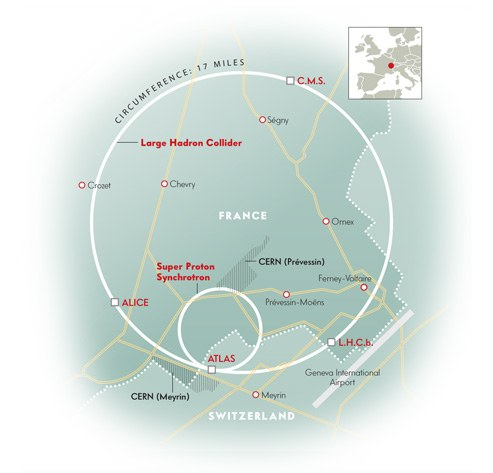
\includegraphics[width=0.95\textwidth]{\figpath/Chapter2/LHC_schematic.jpg}
	\caption{Overhead view of CERN and its main experiments, CMS; ATLAS; LHCb; and ALICE, as well as two of the larger accelerators, the LHC and SPS. The schematic is overlaid on a map of Switzerland and France~\cite{LHC-schematic}.}
	\label{fig:LHC_schematic}
\end{figure}

The LHC provides beams for four main experiments located along its beam line (Fig.~\ref{fig:LHC_schematic}):
\begin{itemize}
	\item The CMS (Compact Muon Solenoid)~\cite{Chatrchyan:2008aa} and ATLAS (A Toroidal LHC ApparatuS)~\cite{1748-0221-3-08-S08003} experiments are both general purpose detectors. Their goals include precision measurements to test the Standard Model and searches for new physics, including the Higgs boson.
	\item LHCb (Large Hadron Collider beauty)~\cite{Alves:2008zz} was designed to do precision measurements of CP-violation and the physics of B-mesons.
	\item ALICE (A Large Ion Collider Experiment)~\cite{Aamodt:2008zz} studies heavy ion collisions.
\end{itemize}

The LHC was designed to collide two beams of protons (pp), heavy ions (PbPb), or a combination of the two (pPb) at specific interaction points around the beam line.
For the purposes of this thesis we will only cover proton-proton collisions from this point forward.
The protons come from a single bottle of hydrogen gas, which is then disassociated and stripped of electrons to form a proton beam.
Interestingly, only 1\unit{ng} of hydrogen is required per day in order to form the LHC beams.
The protons next travel through the Linac2 machine where they form bunched by radio frequency (RF) electromagnetic fields and are accelerated to 50\MeV.
This chain continues through the Proton Synchroton Booster (PSB), the Proton Synchrotron (PS), and the Super Proton Synchrotron (SPS) where the protons are accelerated to 1.4\GeV, 26\GeV, and 450\GeV respectively (Fig.~\ref{fig:CERN_accelerators}).

\begin{sidewaysfigure}[!hbt]
	\centering
	\begin{subfigure}[t]{0.4655\textwidth}
		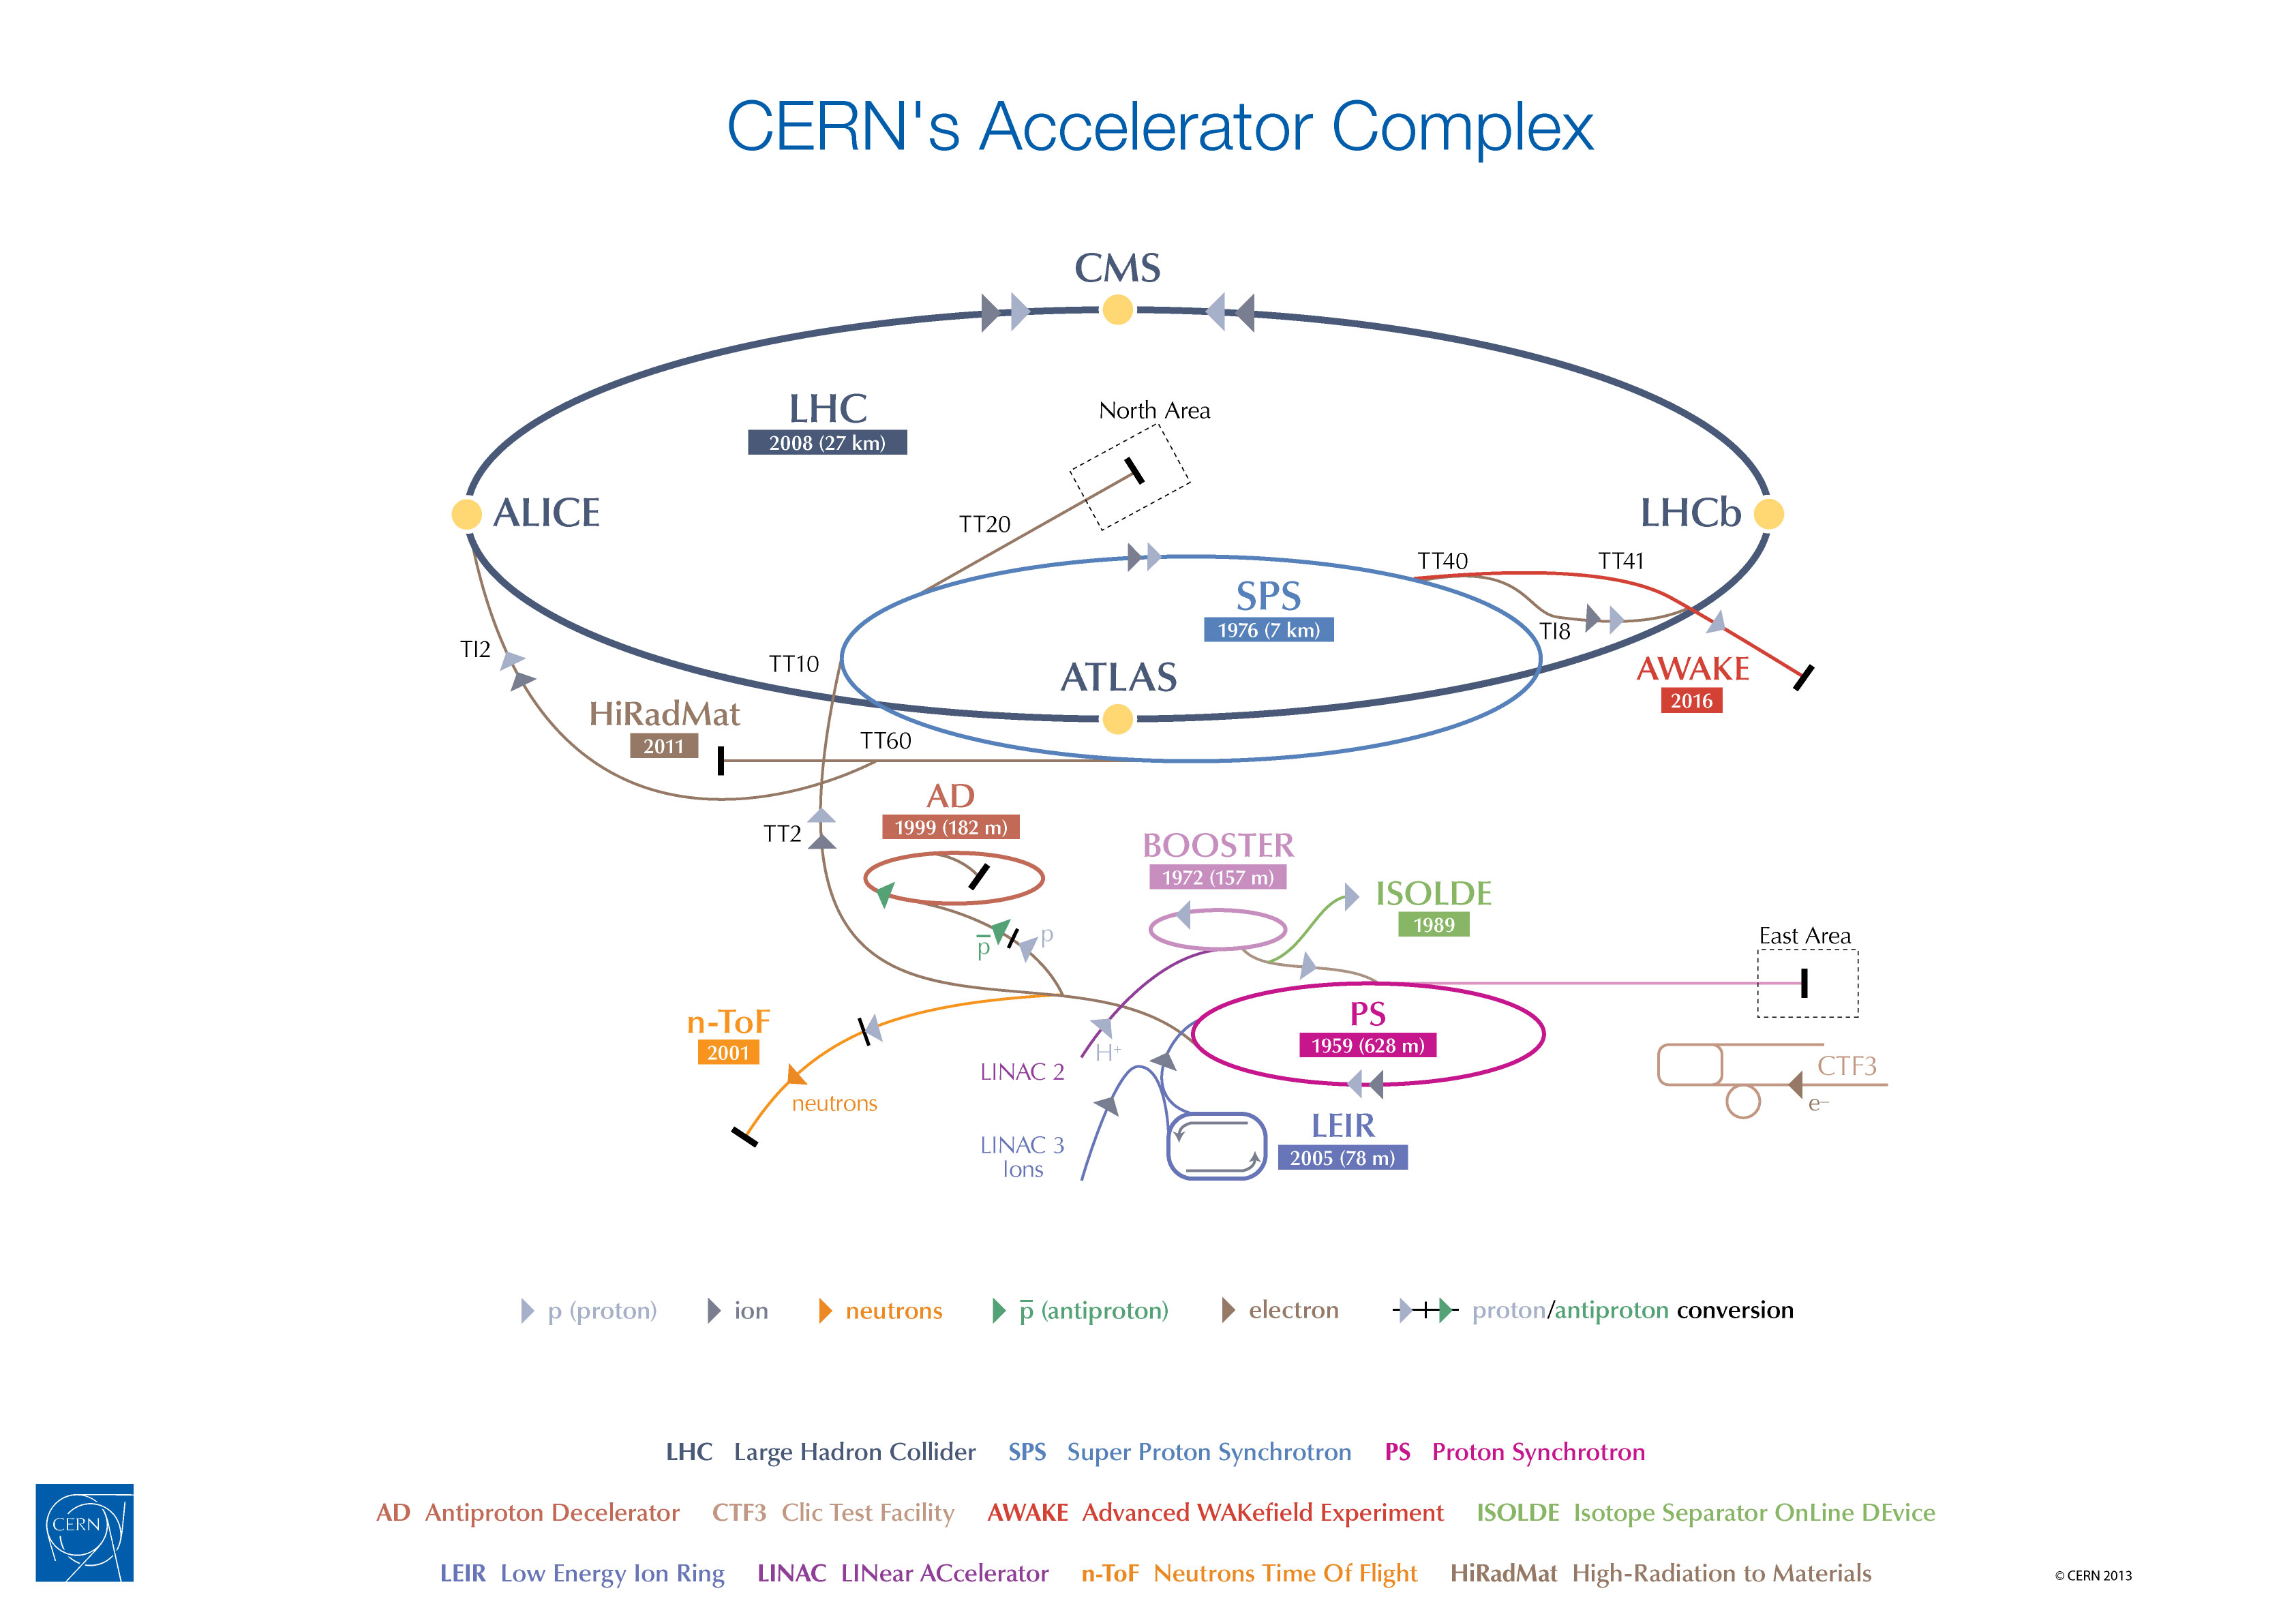
\includegraphics[width=\textwidth]{\figpath/Chapter2/CERN's-accelerator-complex2013.jpg}
		\label{fig:CERN_accelerator_complex}
	\end{subfigure}
	\begin{subfigure}[t]{0.4655\textwidth}
		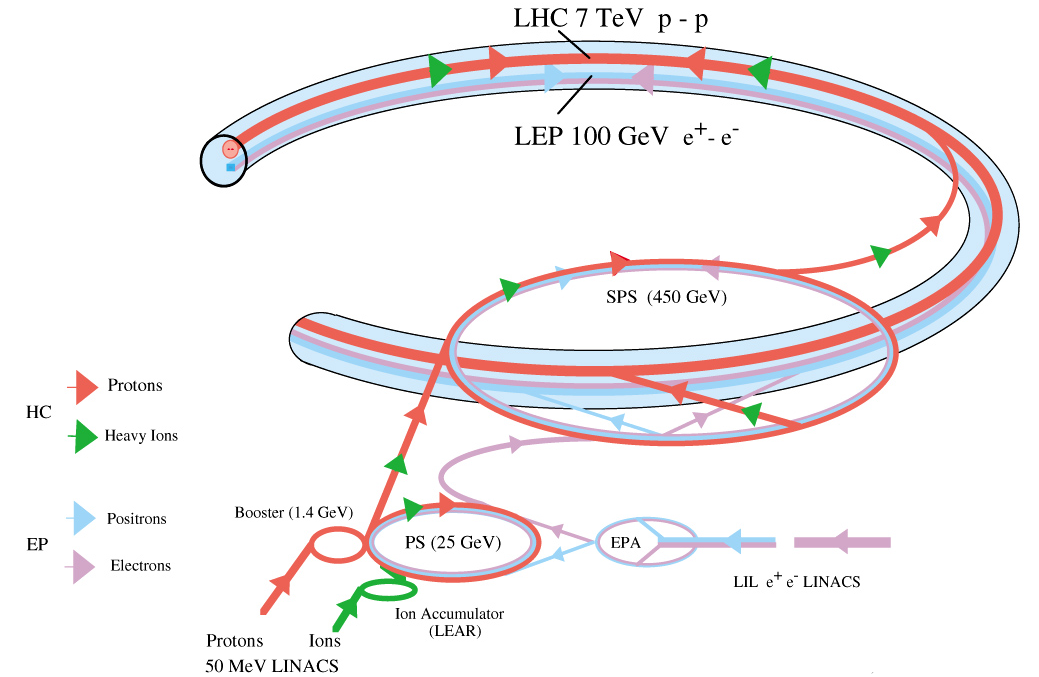
\includegraphics[width=\textwidth]{\figpath/Chapter2/lhc-pho-1993-008.png}
		\label{fig:LHC_LEP_injection_complex}
	\end{subfigure}
	\caption{Left: A schematic of the CERN accelerator complex~\cite{Marcastel:1621583}. Right: A diagram of the LHC injection chain. Also included is a diagram of the heavy ion and LEP injection chains~\cite{Jean-Luc:841568}.}
	\label{fig:CERN_accelerators}
\end{sidewaysfigure}

\clearpage

After being accelerated in the SPS, the proton bunches are injected into the two LHC beam pipes, which were designed to accelerate the two proton beams to 7\TeV (Fig~\ref{fig:LHC_beams}).
Size limitations in the tunnel dictated that the the beam lines be formed by twin bore magnets.
Each magnet is formed by a single mechanical structure and cryostat while containing two coils and two beam channels.
The coils are made out of superconducting NbTi Rutherford cables cooled to 1.9\unit{K} by 120\unit{t} of superfluid helium.
This forms the 8.33\unit{T} magnets necessary for bending the 7\TeV protons (Fig.~\ref{fig:LHC_magnet}).
The LHC contains 1232 superconducting dipole magnets for bending the protons and 392 superconducting quadrupole magnets for focusing the beams.
The beam line also contains sextapole, octopole, and decapole magnets, which are also used to correct and focus beams.
The original LHC design calls for a bunch spacing of 25\unit{ns}, $10^{11}$ protons per bunch, and 2808 bunches per beam.
%The acceleration is accomplished by 16 RF cavities operating at 400MHz.

\begin{figure}[!hbt]
	\centering
	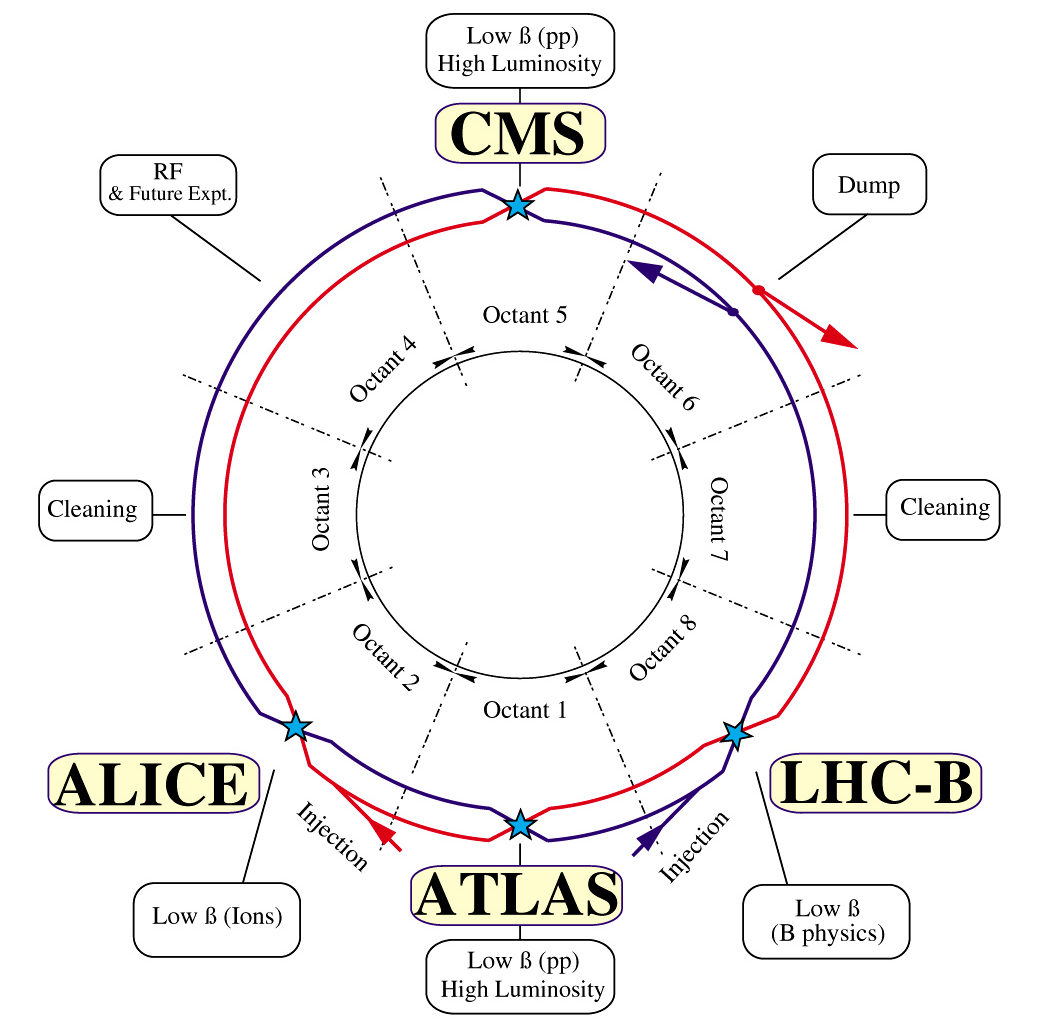
\includegraphics[width=0.95\textwidth]{\figpath/Chapter2/lhc-pho-1997-060.png}
	\caption{A diagram of the LHC beams along with the four major experiments~\cite{Jean-Luc:841573}.}
	\label{fig:LHC_beams}
\end{figure}

\begin{figure}[!hbt]
	\centering
	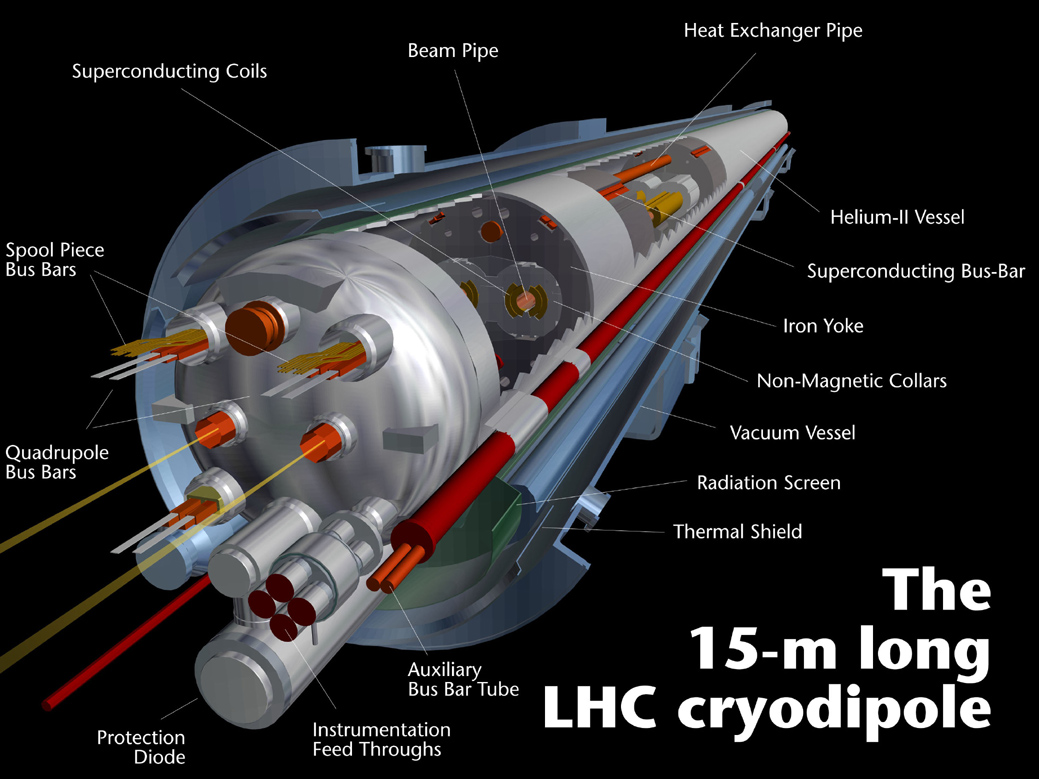
\includegraphics[width=0.95\textwidth]{\figpath/Chapter2/lhc-pho-1998-299.jpg}
	\caption{A diagram of an LHC dipole magnet and cryostat~\cite{Dailler:842253}.}
	\label{fig:LHC_magnet}
\end{figure}

The original plan was to start the LHC accelerator complex in September 2008.
However, due to a catastrophic incident damaging the machine, the startup was delayed until November 23, 2009; even then colliding beams only had a center-of-mass energy of 900\GeV.
From March 30, 2010 through the end of 2011 the LHC operated with a center-of-mass energy of 7\TeV.
Then in 2012 the energy was again increased to 8\TeV (4\TeV per beam), which is the energy of the beams during the data-taking period focused on by this thesis.
It is important to note, though, that the machine has continued to operate after the 2012 data taking period and increased the center-of-mass energy to 13\TeV starting in 2015 (there was a planned shutdown from 2013 through early 2015).

In addition to the center-of-mass energy, collider physicists are interested in the rate at which a specific physics process occurs.
This in turn is related to the cross sections, the probability that two particles will collide and react a certain way, and the luminosity.
The rate of events is given by equation~\ref{eq:dn/dt}, where $\mathcal{L}$ is the collision luminosity and $\sigma$ is the cross section for a given physical process.

\begin{equation}
dN/dt=\mathcal{L}{\cdot}\sigma
\label{eq:dn/dt}
\end{equation}

The luminosity as it is described here is often called the ``instantaneous luminosity'' as this value can change from moment to moment.
The ``integrated luminosity'' is then a measure of the total amount of data collected.
The instantaneous luminosity itself depends upon the parameters of the LHC beams and the optical properties of the focusing system at the interaction point.
This information is summed up in equation~\ref{eq:luminosity}~\cite{1742-6596-455-1-012001}:

\begin{equation}
\mathcal{L}=\frac{N^{2}n_{b}f\gamma}{4\pi\epsilon_{n}\beta^{*}}F
\label{eq:luminosity}
\end{equation}

where:

\begin{itemize}
	\item $N$: protons per bunch
	\item $n_{b}$: bunches in the LHC ring
	\item $f$: frequency of bunch revolutions around the ring 
	\item $\gamma$: relativistic factor for the protons
	\item $\epsilon_{n}$: normalized emittance of the proton beams
	\item $\beta^{*}$: beta function at the interaction point
	\item $F$: geometrical reduction factor due to the crossing angle of the beams
\end{itemize}

The maximum design luminosity of the LHC is $1\times10^{34}\percms$.
During the 2010 and 2011 run periods (7\TeV center-of-mass energy) the instantaneous luminosity increased from $1\times10^{32}\percms$ to $5\times10^{33}\percms$.
During the 2012 data-taking period, the peak instantaneous luminosity was $7.67\times10^{33}\percms$ with a bunch spacing of 50\unit{ns}, a maximum number of bunches of 1380, and $\sim2.2\times10^{14}$ protons per beam ($\sim1.6\times10^{11}$ protons per bunch).
The LHC delivered 23.30\fbinv of integrated luminosity to the CMS detector of which 21.79\fbinv was recorded.
As of the end of 2016, the LHC is still running at 13\TeV (6.5\TeV per beam) with a peak luminosity of $1.53\times10^{34}\percms$, 2208 bunches, and $1\times10^{11}$ protons per bunch~\cite{CMSWebBasedMonitoring,LumiPublic}.
Figures~\ref{fig:LHC_int_lumi_pp} and~\ref{fig:LHC_lumi_per_day_pp} show the total integrated luminosity delivered by the LHC and recorded by the CMS experiment for the various data-taking periods~\cite{LumiPublic}.

\begin{figure}[!hbt]
	\centering
	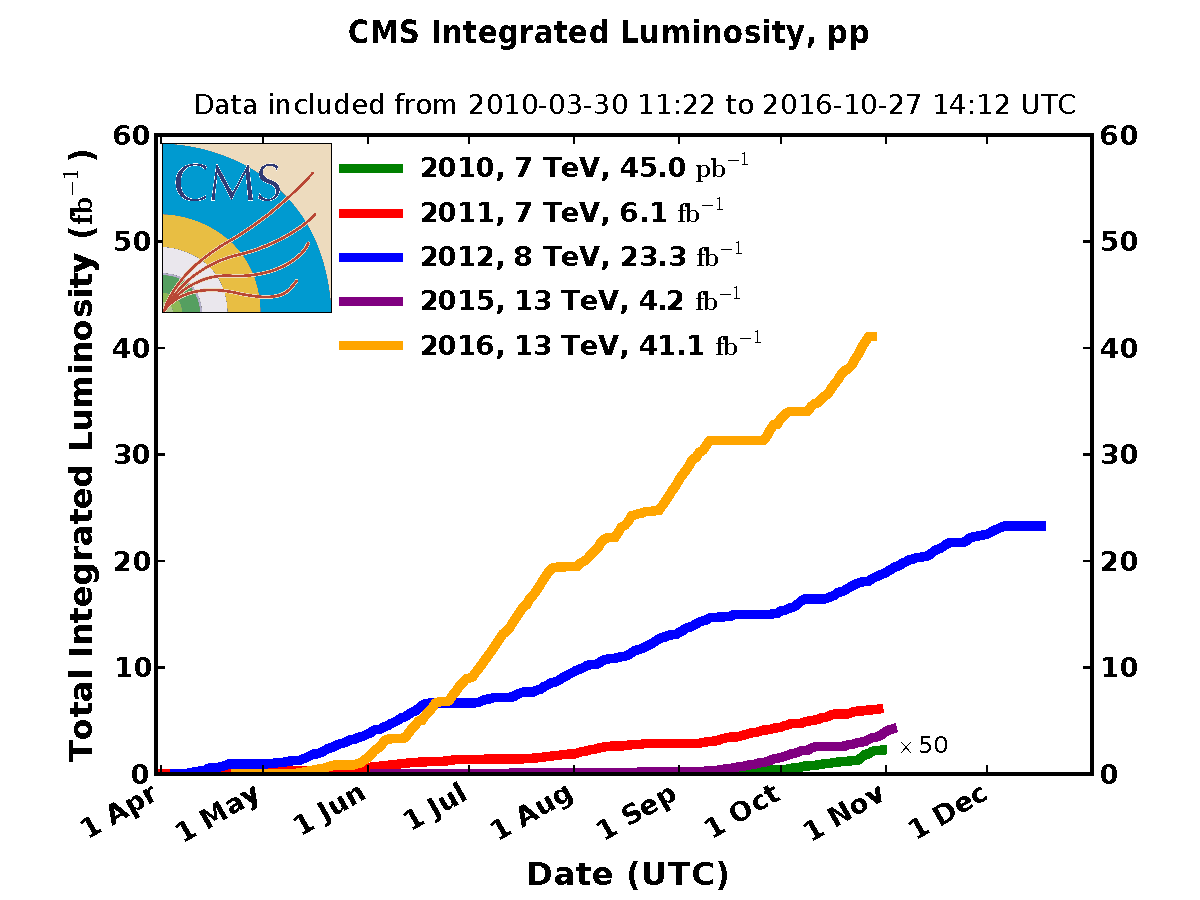
\includegraphics[width=0.95\textwidth]{\figpath/Chapter2/int_lumi_cumulative_pp_2.pdf}
	\caption{Total integrated luminosity versus time delivered to the CMS experiment for the 2010, 2011, 2012, 2015, and 2016 p-p data-taking periods~\cite{LumiPublic}.}
	\label{fig:LHC_int_lumi_pp}
\end{figure}

\begin{figure}[!hbt]
	\centering
	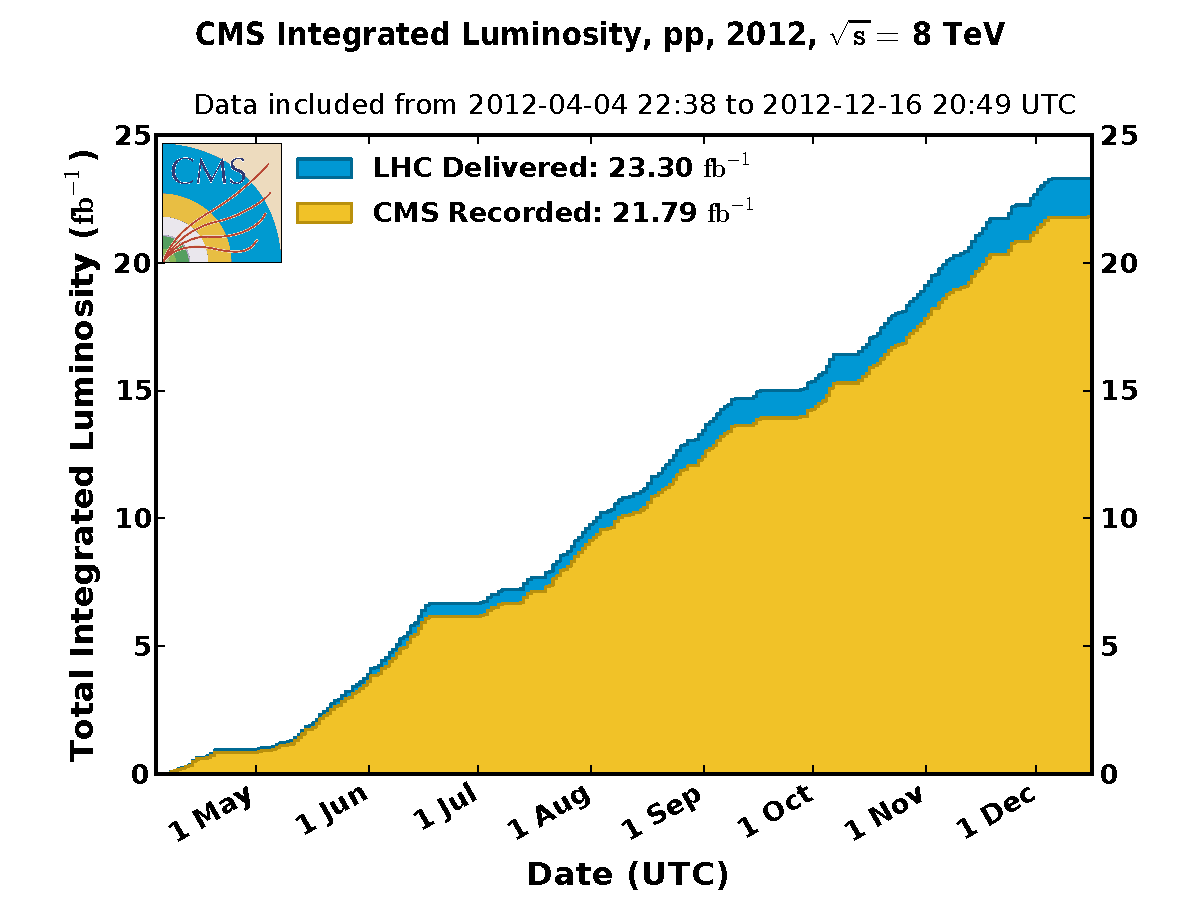
\includegraphics[width=0.95\textwidth]{\figpath/Chapter2/int_lumi_per_day_cumulative_pp_2012.pdf}
	\caption{Total integrated, offline luminosity versus day in 2012. The blue graph shows the delivered luminosity while the orange graph shows the luminosity recorded by the CMS experiment. This graph shows only the luminosity collected for p-p collisions during stable beams~\cite{LumiPublic}.}
	\label{fig:LHC_lumi_per_day_pp}
\end{figure}


\section{The CMS Detector}

TALK ABOUT THE PHYSICS GOALS?
%"The physics program of the experiment covers a wide range of goals: precision study of Standard Model processes, study of properties of the recently discovered Higgs boson, searches for physics beyond the Standard Model, and study of quark-gluon plasma." - Aysen Tatarinov

The CMS experiment is one of two general purpose detectors at the LHC; ATLAS being the other one.
The detector is located 100\unit{m} underground near Cessy, France on the opposite side of the LHC from the main CERN site in Meyrin (see figure~\ref{fig:LHC_schematic}).
It was largely built on the surface and then lowered into the collision cavern in 15 pieces, which then had to be painstakingly assembled.
The detector has a cylindrical design which is 22\unit{m} in length, 15\unit{m} in diameter, and weights 14000 tonnes.
The shape and positioning of the detector around the interaction point (IP) gives the experiment nearly $4\pi$ coverage of the proton collisions.
The layout of the detector can be seen in fig.~\ref{fig:CMS_schematic}.

\begin{figure}[!hbt]
	\centering
	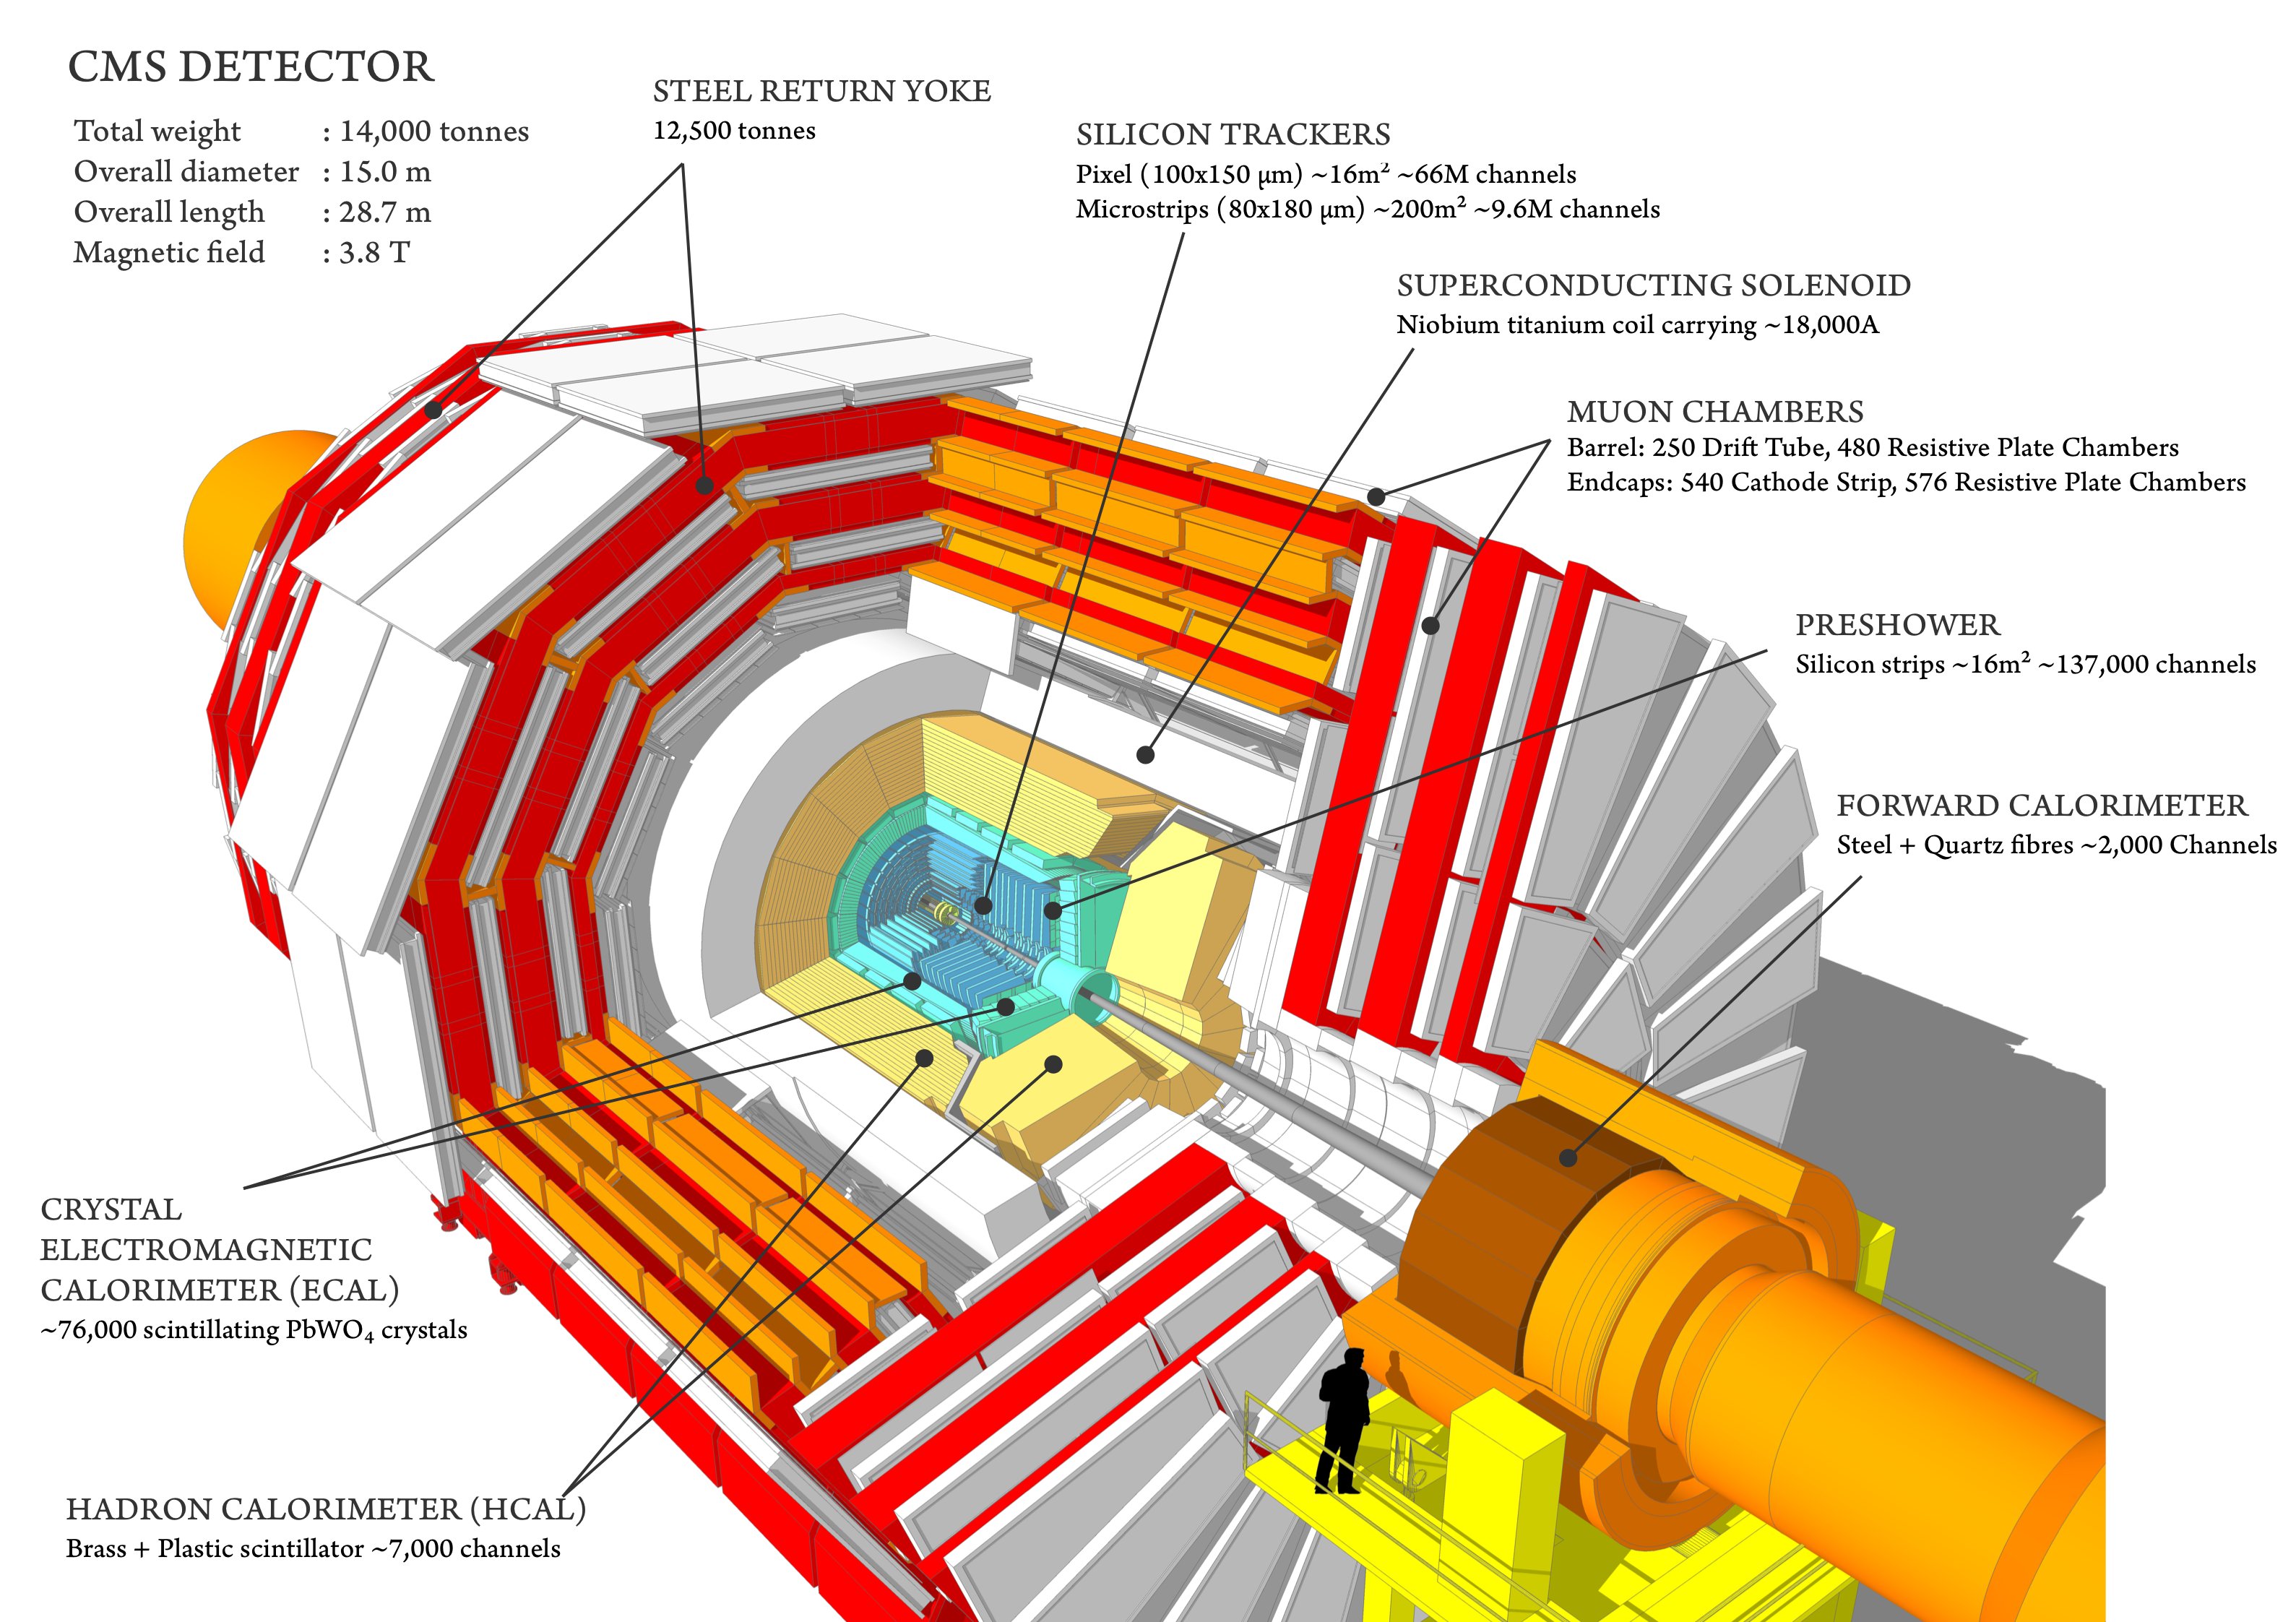
\includegraphics[width=0.95\textwidth]{\figpath/Chapter2/cms_160312_02.png}
	\caption{Schematic of the CMS detector with labels and notable figures~\cite{SketchUpCMS}.}
	\label{fig:CMS_schematic}
\end{figure}

Fig.~\ref{fig:CMS_transverse} shows how various types of particles interact within the CMS sub-detectors.
In total, there are ${\sim}10^8$ data channels checked in each bunch crossing owing to the high granularity of the CMS sub-detectors.
The following sections will describe each of the sub-detectors and its properties and is based largely on Ref.~\cite{Chatrchyan:2008aa}.

\begin{figure}[!hbt]
	\centering
	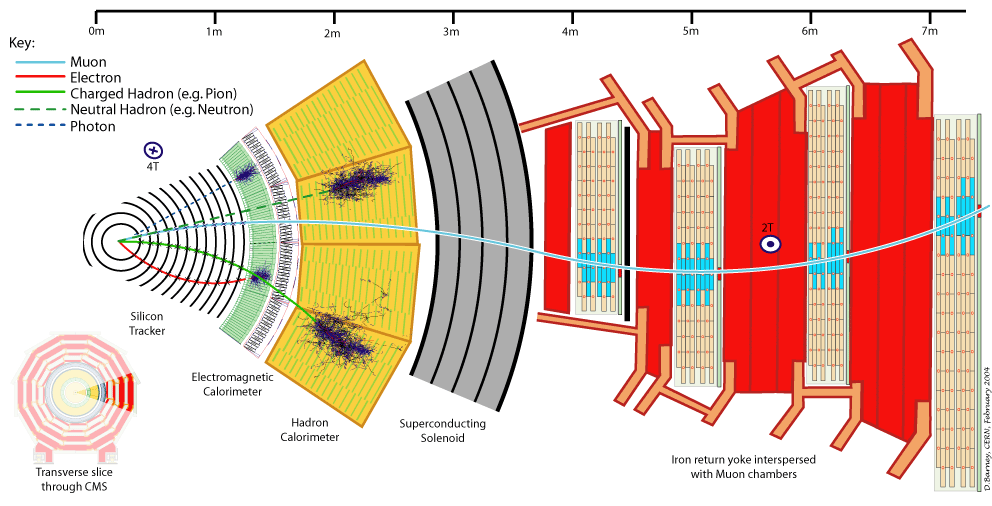
\includegraphics[width=0.95\textwidth]{\figpath/Chapter2/CMS_slice.png}
	\caption{Transverse slice of the CMS experiment with the major sub-detectors and components represented. The different colored lines represent how various types of particles interact with the sub-detectors~\cite{CMSSlice}.}
	\label{fig:CMS_transverse}
\end{figure}

\subsection{Coordinate System}

The IP is at the center of the detector and is the origin of the right-handed coordinate system used to describe the detector and the physics being measured (location and direction).
The $z$-axis is defined along the LHC beam line.
Instead of using the polar angle, $\theta$, which would go from $0^{\degree}$ along the positive $z$-axis to $90^{\degree}$ pointing straight up from the interaction point, collider physicists use the quantity pseudorapidity defined as $\eta=-ln\left[\tan\left(\theta/2\right)\right]$.
The benefits of using the pseudorapidity are that differences in this coordinate, $\Delta\eta$, are invariant under boosts in the $z$-direction and particle production is roughly uniform in $\eta$.
The $x$- and $y$-axes form the plane perpendicular to the $z$-axis, where positive $x$ points to the center of the LHC ring and positive $y$ points upward.
The azimuthal angle, $\phi$, and radial coordinate, $r$, are also defined in this same plane.
It is sometimes more useful to use $\phi$ and $r$ due to the bending of the particles in the magnetic field.
Lastly, this paper will often refer to the quantity \pt, which is the magnitude of the component of the momentum vector in the transverse plane.
A schematic of the coordinate system described above is shown in fig.~\ref{fig:CMS_coordinate_system}.

\begin{figure}[!hbt]
	\centering
	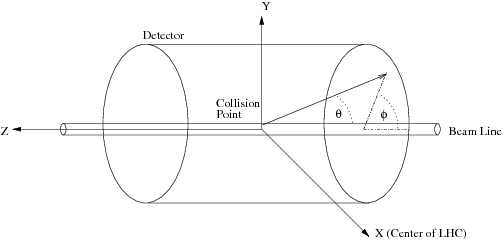
\includegraphics[width=0.95\textwidth]{\figpath/Chapter2/Figures_T_Coordinate.png}
	\caption{Schematic of the CMS coordinate system~\cite{Schott:2014sea}.}
	\label{fig:CMS_coordinate_system}
\end{figure}

\subsection{Tracker and Pixel Detector}
\label{sec:tracker_and_pixel}

The CMS all-silicon tracker is the closest sub-detector to the LHC beam pipe.
It is 5.8\unit{m} long and 2.5\unit{m} in diameter, covering a pseudorapidity range of $\abs{\eta}<2.5$.
It is, by necessity, highly granular, to keep the occupancy low, and relatively radiation hard.
The tracker is exposed to extreme doses of radiation ranging from 0.18 to 84\unit{Mrad} after 500\fbinv of data.
The radiation tolerance was a key factor in determining the materials and design of the sensors and on-board electronics of the tracker.
To keep the radiation damage as low as possible, among other benefits, the tracker is kept at $-10\degC$.
For non-isolated particles of $1<\pt<10\GeV$ and $\abs{\eta}<1.4$, the track resolutions are typically 1.5\% in \pt and 25--90 (45--150)\mum in the transverse (longitudinal) impact parameter.
On the other hand, isolated particles of $\pt=100\GeV$ emitted at $\abs{\eta}<1.4$ have track resolutions of 2.8\% in \pt and 10 (30)\mum in the transverse (longitudinal) impact parameter~\cite{TRK-11-001}.
At higher $\eta$ the reduced transverse depth of the tracker degrades the resolution (particles traverse fewer layers).
Fig.~\ref{fig:CMS_tracker} shows the layout of the tracker and its subsystems. The tracker is formed by two major subsystems, the pixel detector and the silicon strip tracker.


\begin{figure}[!hbt]
	\centering
	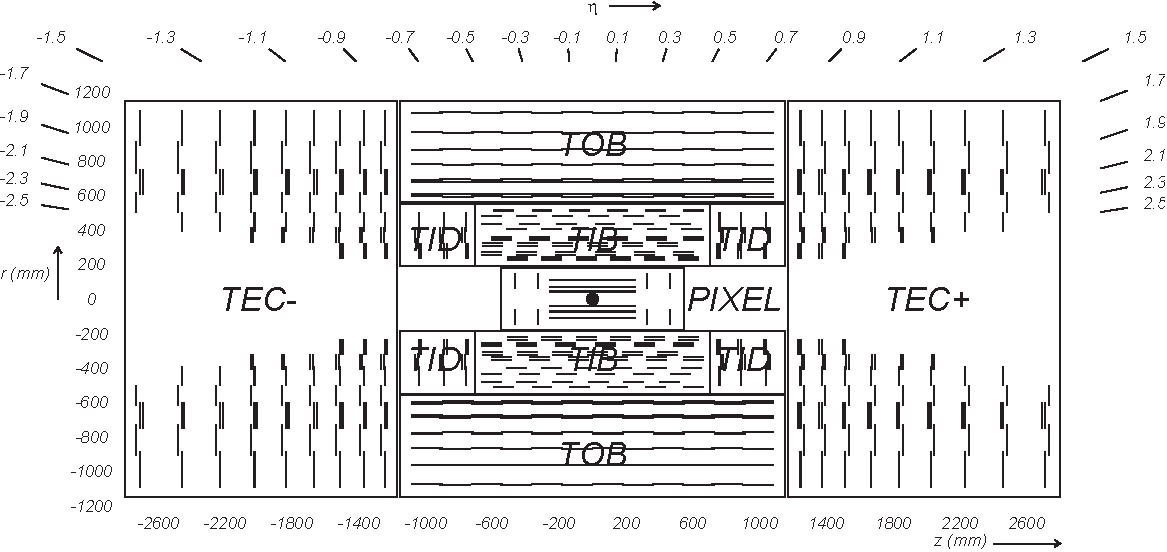
\includegraphics[width=0.95\textwidth]{\figpath/Chapter2/CMS_tracker.pdf}
	\caption{Layout of the CMS tracker with subsystems labeled.}
	\label{fig:CMS_tracker}
\end{figure}

The pixel detector is made up of three barrel layers, called the BPIX, and two endcap layers called the FPIX.
The BPIX contains 48 million pixels and the FPIX contains another 18 million pixels.
In total it consists of 1440 hybrid silicon detector modules, each with a dimension of $100\times150\mum^{2}$.
The small pixel size enables track resolutions of 10\mum in the transverse plane and 20\mum in the $z$-direction.
The pixel detector is what gives CMS its excellent secondary vertex tagging ability in addition to producing seed tracks for the strip tracker and the high level trigger.
NOT SURE I LIKE THIS LAST SENTENCE

Just as the pixel detector was made up of the BPIX and FPIX subsystems, the silicon strip detector is made up of four subsystems.
The Tracker Inner Barrel
(TIB) has four layers of 320\mum strips.
At each end of the TIB is a three-layer Tracker Inner Disks (TID), which contains strips of the same thickness.
The Tracker Outer Barrel (TOB) is the six layer system which surrounds the TIB/TID.
The first four layers of the TOB use 500\mum thick strips, and the last two layers use 122\mum thick strips.
The Tracker EndCaps (TEC) are on either side of the previous setup and contains nine disks with up to seven layers of strips.
These strips are 320\mum thick in the inner four rings and 500\mum thick in the outer three rings.
In total, the strip detector contains 9.3 million silicon strips (15\,148 modules).

The 2012 LHC run was an excellent year for the tracker.
The BPIX maintained 97.7\% of its channels operational while the FPIX had 92.8\% of its channels operational.
The reconstruction efficiencies were also quite high, 99.5\%, for each later of the pixel detector ($>$99.2\% for the first layer).
The strip detector maintained 97.5\% of its channels active and had a reconstruction efficiency greater than 99\% for each layer\cite{Veszpremi:2014hpa}. 

\subsection{Electromagnetic Calorimeter}

The electromagnetic calorimeter (ECAL) is a homogeneous detector consisting entirely of 75\,848 lead tungstate crystals (\PbWO).
The detector is divided up into two sections which provide coverage in pseudorapidity \absetalt{1.479} in a barrel region (EB) and \abseta{1.479}{3.0} in two endcap regions (EE).
There are also preshower detectors (PS) in each of the endcaps, in front of the EE, which cover a pseudorapidity range of \abseta{1.653}{2.6}.
Fig.~\ref{fig:CMS_ECAL} shows the structure of the detector with the key $\eta$ values labeled.

\begin{figure}[!hbt]
	\centering
	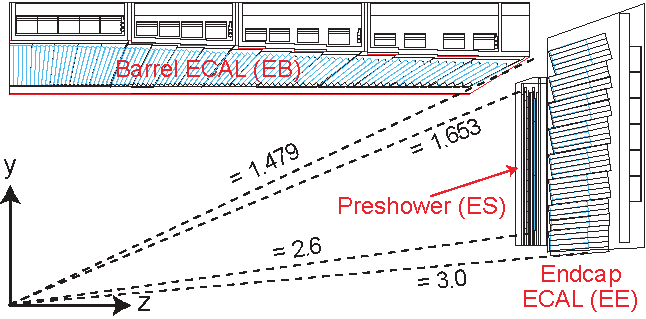
\includegraphics[width=0.95\textwidth]{\figpath/Chapter2/ECAL_transverse_section.pdf}
	\caption{A schematic of the CMS ECAL detect with labeled subsystems and key $\eta$ ranges marked.}
	\label{fig:CMS_ECAL}
\end{figure}

The barrel region of the ECAL consists of 61\,200 crystals with a tapered shape arranged in a projective geometry. Each crystal is about \mytimes{0.0174}{0.0174} in $\eta-\phi$, which corresponds to \mytimes{22}{22}\unit{mm$^{\text{2}}$} at the front face and \mytimes{26}{26}\unit{mm$^{\text{2}}$} at the back face. Each crystal has a depth of 230\mm, which for \PbWO corresponds to 25.8 radiation lengths ($X_{0}$). The scintillation light produced in the crystals is read out by avalanche photodiodes (APDs), which produce approximately 4.5 photoelectrons per \MeVns at 18\degC. The dark current of the APDs is sensitive to radiation exposure. During the 2012 run, the dark current ranged from 0.13 to 1.3\muA on average, which corresponds to an average noise of 47 to 57\mev~\cite{CMS:2013ecal}.

The EE contains 14\,648 \PbWO crystals arranged in a non-projective $x-y$ geometry (see fig.~\ref{fig:CMS_ECAL}). The crystal dimensions are \mytimes{28.62}{28.62}\unit{mm$^{\text{2}}$} at the front face and \mytimes{30}{30}\unit{mm$^{\text{2}}$} at the back face with a depth of 220\mm or 24.7 $X_{0}$. Instead of using APDs link in the EB, the EE uses vacuum phototriodes (VPTs) to read out the scintillation light. Again holding the photodetectors at 18\degC, the phototriodes produce 4.5 photoelectrons per \MeVns. The average noise in the VPTs for 2012 was 180--200\mev, but it could reach 600\mev at high $\eta$ due to the higher radiation doses in the more forward regions~\cite{CMS:2013ecal}.

The ES is located in front of each of the EE detectors. It consists of two planes of silicon strip sensors interleaved with a total of $3 X_0$ of lead absorber (2 $X_{0}$ for the first layer and 1 $X_{0}$ for the second layer). The silicon strips are 320\mum thick and can collect 3.6\unit{fC} of charge from a minimum ionizing particle (MIP).

One of the main goals of the CMS experiment was to discover the Higgs boson.
Because of its low irreducible standard model background, the $H\rightarrow\gamma\gamma$ channel was considered the ``golden channel''.
Due to this, a significant amount of money and time was spent on the design and the materials for the ECAL.
\PbWO is a great choice for an ECAL because its properties, listed in table~\ref{tab:PbWO4Properties}, lead to a precision energy measurement for EM objects (by this I mean a fine small resolution). 

\DTLnewdb{PbWO4Data}
\DTLnewrow{PbWO4Data}%
\DTLnewdbentry{PbWO4Data}{Property}{Peak emission wavelength}%
\DTLnewdbentry{PbWO4Data}{Value}{425\unit{nm}}%
\DTLnewrow{PbWO4Data}%
\DTLnewdbentry{PbWO4Data}{Property}{High density}%
\DTLnewdbentry{PbWO4Data}{Value}{8.28\unit{g/cm$^{\text{3}}$}}%
\DTLnewrow{PbWO4Data}%
\DTLnewdbentry{PbWO4Data}{Property}{Short radiation length}%
\DTLnewdbentry{PbWO4Data}{Value}{0.89\unit{cm}}%
\DTLnewrow{PbWO4Data}%
\DTLnewdbentry{PbWO4Data}{Property}{Short Moli\`{e}re radius}%
\DTLnewdbentry{PbWO4Data}{Value}{2.2\unit{cm}}%
\DTLnewrow{PbWO4Data}%
\DTLnewdbentry{PbWO4Data}{Property}{Fast decay time}%
\DTLnewdbentry{PbWO4Data}{Value}{6\unit{ns}}%
%\dtlsort{Property}{PbWO4Data}{\dtlcompare}

\begin{table}[htbp]
\caption{\PbWO properties and their measured values}
\centering
\begin{tabular}{|l|c|}%
\dtldisplaystarttab
Property & Value %
\DTLforeach
*
{PbWO4Data}{}{%
\gdef\doamp{\gdef\doamp{&}}%
\DTLiffirstrow{\\\hline}{\\}%
\DTLforeachkeyinrow{\thisValue}{\doamp\thisValue}}%
\dtldisplayendtab
\end{tabular}
\label{tab:PbWO4Properties}
\end{table}

The energy resolution, $\sigma$, of deposits in the ECAL vary as a function of energy ($E$) (in units of \unit{\gev}).
This is typically modeled using an NSC function as in equation~\ref{eq:ECAL_NSC}:

\begin{equation}
\label{eq:ECAL_NSC}
\left(\frac{\sigma}{E}\right)^{2}=\left(\frac{N}{E}\right)^{2}+\left(\frac{S}{\sqrt{E}}\right)^{2}+C^{2}
\end{equation}

\noindent where $N$ is the noise term, $S$ is the stochastic term, and $C$ is the constant term.
Typical values for these terms come from test beam studies and are listed in table~\ref{tab:ECAL_NSC}~\cite{CMS:2013ecal}.
In the barrel section of the ECAL, an energy resolution of about 1\% is achieved for unconverted or late-converting photons in the tens of GeV energy range.
The remaining barrel photons have a resolution of about 1.3\% up to a pseudorapidity of \absetaeq{1}, rising to about 2.5\% at \absetaeq{1.4}.
In the endcaps, the resolution of unconverted or late-converting photons is about 2.5\%, while the remaining endcap photons have a resolution between 3\% and 4\%~\cite{CMS:EGM-14-001}.

\begin{table}[htbp]
\caption{Typical values for the noise, stochastic, and constant terms of the ECAL energy resolution function. These values are obtained from test beam studies.}
\centering
\begin{tabular}{|l|c|}%
\hline %
Term & Typical Value \\%
\hline
N & 12\% \\%
S & 2.8\% \\%
C & 0.30\% \\%
\hline
\end{tabular}
\label{tab:ECAL_NSC}
\end{table}

\subsection{Hadron Calorimeter}
\label{sec:hadron_calorimeter}

The CMS hadron calorimeter (HCAL) is, as its name suggests, designed to measure the energy of hadrons.
This is especially important for neutral hadrons which leave no tracks and, to a large extent, do not register in the ECAL.
The HCAL is a sampling calorimeter, meaning that is contains both an active, energy measurement material as well as a material which induces the hadrons to shower.
The HCAL is made up of four subsystem: HCAL barrel (HB), HCAL endcap (HE), HCAL outer (HO), and HCAL forward (HF).
The HB, HE, and HO subsystems all use the same technology, while the HF uses a different technology.
Fig.~\ref{fig:CMS_HCAL} shows the structure and position of the HCAL subsystems.
When both the ECAL and HCAL work together, the CMS calorimeters can measure a charged pion with a resolution of $\sigma/E\approx100\%/\sqrt{E[GeV]}\oplus5\%$, where $E$ is the jet energy.

\begin{figure}[!hbt]
	\centering
	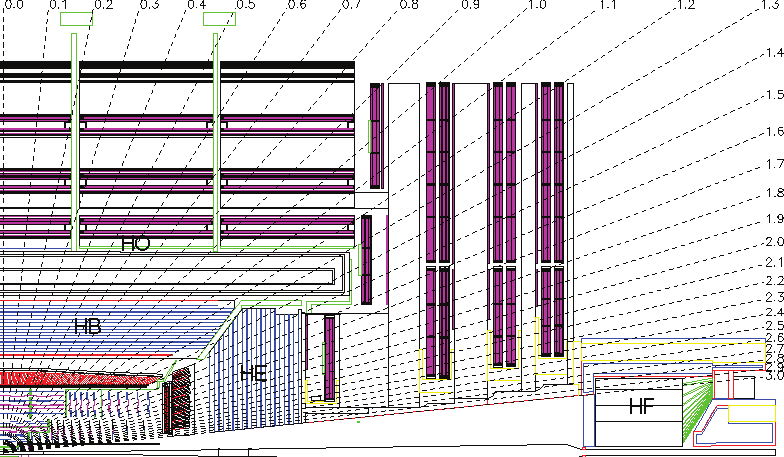
\includegraphics[width=0.95\textwidth]{\figpath/Chapter2/HCAL_subdet.pdf}
	\caption{A schematic of the CMS HCAL detector with its major subsystems labeled: HB, HE, HO, and HF.}
	\label{fig:CMS_HCAL}
\end{figure}

The HB occupies the region \absetalt{1.3} and contains alternating layers of brass and scintillator.
The number of nuclear interaction lengths ($\lambda_{0}$) ranges from 5.82 at $\eta=0$ to 10.6 at $\eta=1.3$.
Additionally the EB, which is directly in front of the HB, has 1.1$\lambda_{0}$ and can measure a portion of early developing hadronic showers, though not as accurately.
The properties of the brass used can be found in table~\ref{tab:HCAL_brass_properties} while the layer thicknesses and materials can be found in table~\ref{tab:HCAL_brass_thickness}.
Most of the plastic scintillating layers are 3.7\unit{mm} thick, but layer 16 is 9\unit{mm} thick so that is can sample more from late developing showers.
There is also an additional 9\unit{mm} thick layer 0 before the first absorbing layer so catch the showers which are initiated in the dead material between the EB and HB.
The scintillating tiles are arranged in a projective geometry (pointing close to the nominal interaction point) with the tiles occupying \mytimes{0.087}{0.087} in $\eta-\phi$.
For \absetalt{1.479}, the HCAL cells map on to $5\times5$ arrays of ECAL crystals to form calorimeter towers.
Within each tower, the energy deposits in ECAL and HCAL cells are summed to define the calorimeter tower energies, subsequently used to provide the energies and directions of hadronic jets.
The scintillator is separated into 16 $\eta$ section and 36 $\phi$ sections with almost 70000 tiles used.
The light is collected by wavelength shifting (WLS) fibers that encircle the tiles.
Fibers from several layers are read out by one hybrid photodiode (HPD), which are used for their large dynamic range and low sensitivity to magnetic fields.

\begin{table}[htbp]
\caption{Properties of the brass absorber used for the CMS HB.}
\centering
\begin{tabular}{|l|c|}%
\hline %
Property & Value \\%
\hline
Materials & Brass (70\% Copper and 30\% Zinc) or Steel \\%
Density & 8.53\unit{g/cm$^{\text{3}}$}\% \\%
Radiation Length & 1.49\unit{cm} \\%
Nuclear Interaction Length & 16.42\unit{cm}\\
\hline
\end{tabular}
\label{tab:HCAL_brass_properties}
\end{table}

\begin{table}[htbp]
\caption{Absorbing layer thicknesses and materials for the CMS HB}
\centering
\begin{tabular}{|l|c|c|}%
\hline %
Layer number(s) & Material & Thickness (\unit{mm}) \\%
\hline
1 & Steel & 40 \\%
2-9 & Brass & 50.5 \\%
10-15 & Brass & 56.5 \\%
16 & Steel & 75 \\%
\hline
\end{tabular}
\label{tab:HCAL_brass_thickness}
\end{table}

In the central region of the detector there are too few $\lambda_{0}$ to fully contain a hadronic shower.
For this reason the HO system was added as a scintillating tile extension to the HB.
The HO consists of five rings, each with a width of 2.536\unit{m} in the $z$-direction.
The most central ring, Ring 0, has two scintillating layers, one inside the solenoid and one outside the solenoid.
The other rings have only one layer outside of the solenoid, which acts as a 19.5\unit{cm} iron absorber layer.
This addition to the HB brings the total depth of the CMS calorimeter systems to 11.8$\lambda_{0}$.

The HE, a 17 layer sampling calorimeter, covers the \abseta{1.3}{3.0} region.
It consists of 79\unit{mm} brass absorbing layers and uses the same scintillating material as is used in the HB, but contains only 20916 tiles.
Within \absetalt{1.6} the granularity of these tiles is the same as for the HB, but at higher $\eta$ the approximate granularity becomes \mytimes{0.174}{0.174} in $\eta-\phi$.
Like the HB, the HE also has a layer 0.
However, unlike the HB, the scintillating layers in the HE are grouped into ``depths'' before the light reaches the HPDs.
Fig~\ref{fig:CMS_HCAL_depth} shows a schematic of the CMS HCAL system where the different colors corresponds to the various depths.
This depth segmentation allows fore more precise recalibration of the HE, which receives a higher radiation dose than the HB.
When combined with the EE, this section of the detector corresponds to a length of 10$\lambda_{0}$.

\begin{figure}[!hbt]
	\centering
	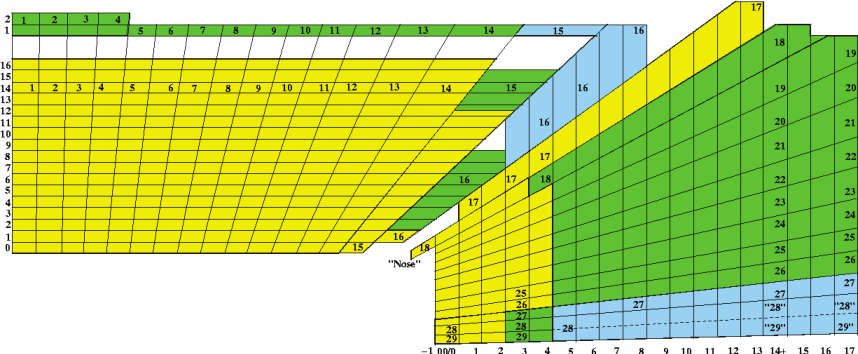
\includegraphics[width=0.95\textwidth]{\figpath/Chapter2/HCAL_tower_segmentation.pdf}
	\caption{A schematic of the HB and HE depth segmentation.}
	\label{fig:CMS_HCAL_depth}
\end{figure}

The HF uses steel as an absorber and embedded quartz fibers as the sensitive material.
The reason for the change in technology is that the HF needs to be able to withstand at least 100\unit{Mrad/year}.
The two halves of the HF are located 11.2\unit{m} from the interaction region, one on each end, and together they provide coverage in the range $3.0<\abs{\eta}<5.2$.
Unlike the other hadronic calorimeter systems, the HF does not have a piece of the ECAL in front of it.
Each HF calorimeter consist of 432 readout towers, containing almost 1000\unit{km} of 800\mum diameter long and short quartz fibers running parallel to the beam with a granularity of \mytimes{0.175}{0.175} in $\eta-\phi$.
The long fibers run the entire depth of the HF calorimeter (165\unit{cm}, or approximately 10 interaction length), while the short fibers start at a depth of 22\unit{cm} from the front of the detector.
By reading out the two sets of fibers separately, it is possible to distinguish EM showers generated by electrons and photons, which deposit a large fraction of their energy in the long-fiber calorimeter segment, from those generated by hadrons, which produce on average nearly equal signals in both calorimeter segments.
The fibers make use of Cherenkov light read out by photomultiplier tubes (PMTs), which receive approximately 1 photoelectron for every 4\gev of deposited energy.

\subsection{Solenoid}

The central feature of the CMS apparatus is a superconducting solenoid of 6\unit{m} internal diameter, providing a magnetic field of 3.8\unit{T}.
The solenoid thus surrounds both the barrel and endcap parts of the silicon pixel and strip tracker, the ECAL, and the HCAL.
The high magnetic field allows CMS to have a relatively small size while also having sufficiently high bending of the high energy charged particles to measure their momenta in the tracker.

The magnet itself is made up of a 4-layer winding of reinforced NbTi superconductor cooled to 4.5\unit{K}.
Like the rest of CMS, this system needed to be modular and is constructed of 5 rings of equal length.
The cold mass of the magnet is 220 tonnes and it stores 2.35\unit{GJ} when the current is fully on.
Fig.~\ref{fig:CMS_solenoid} shows an artist's rendering of the solenoid.

\begin{figure}[!hbt]
	\centering
	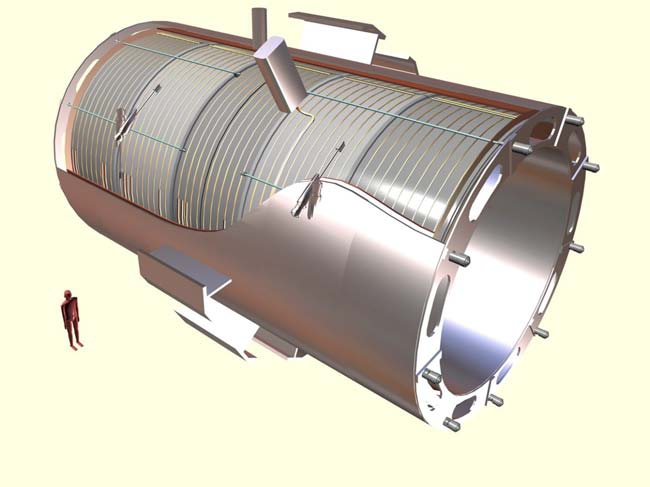
\includegraphics[width=0.95\textwidth]{\figpath/Chapter2/CMS_solenoid.jpg}
	\caption{An artists rendering of the CMS solenoid. The five superconducting rings can be seen inside the cryostat and support structure. A human figure is shown for comparison.}
	\label{fig:CMS_solenoid}
\end{figure}

\subsection{Muon System}

Muons are measured in gas-ionization detectors embedded in the steel flux-return yoke outside the solenoid in the pseudorapidity range \absetalt{2.4}, with detection planes made using three technologies: drift tubes (DTs), cathode strip chambers (CSCs), and resistive plate chambers (RPCs).
The barrel region of the detector contains DTs and RPCs, while the endcap region contains CSCs and RPCs.
The layout of the muon system can be seen in fig.~\ref{fig:CMS_muon_system}.
The iron yoke not only returns the flux from the solenoid, but also shields the muon chambers from stray hadrons.
The entire muon detection system has nearly 1 million electronic channels and weights in excess of 10000 tons.
The muon system on its own has a resolution of 15--40\% depending on $\abs{\eta}$.
Matching muons to tracks measured in the silicon tracker results in a relative transverse momentum resolution for muons with \ptrange{20}{100}\GeV of 1.3--2.0\% in the barrel and better than 6\% in the endcaps. The $p_{T}$ resolution in the barrel is better than 10\% for muons with \pt up to 1\TeV~\cite{Chatrchyan:2012xi}.

\begin{figure}[!hbt]
	\centering
	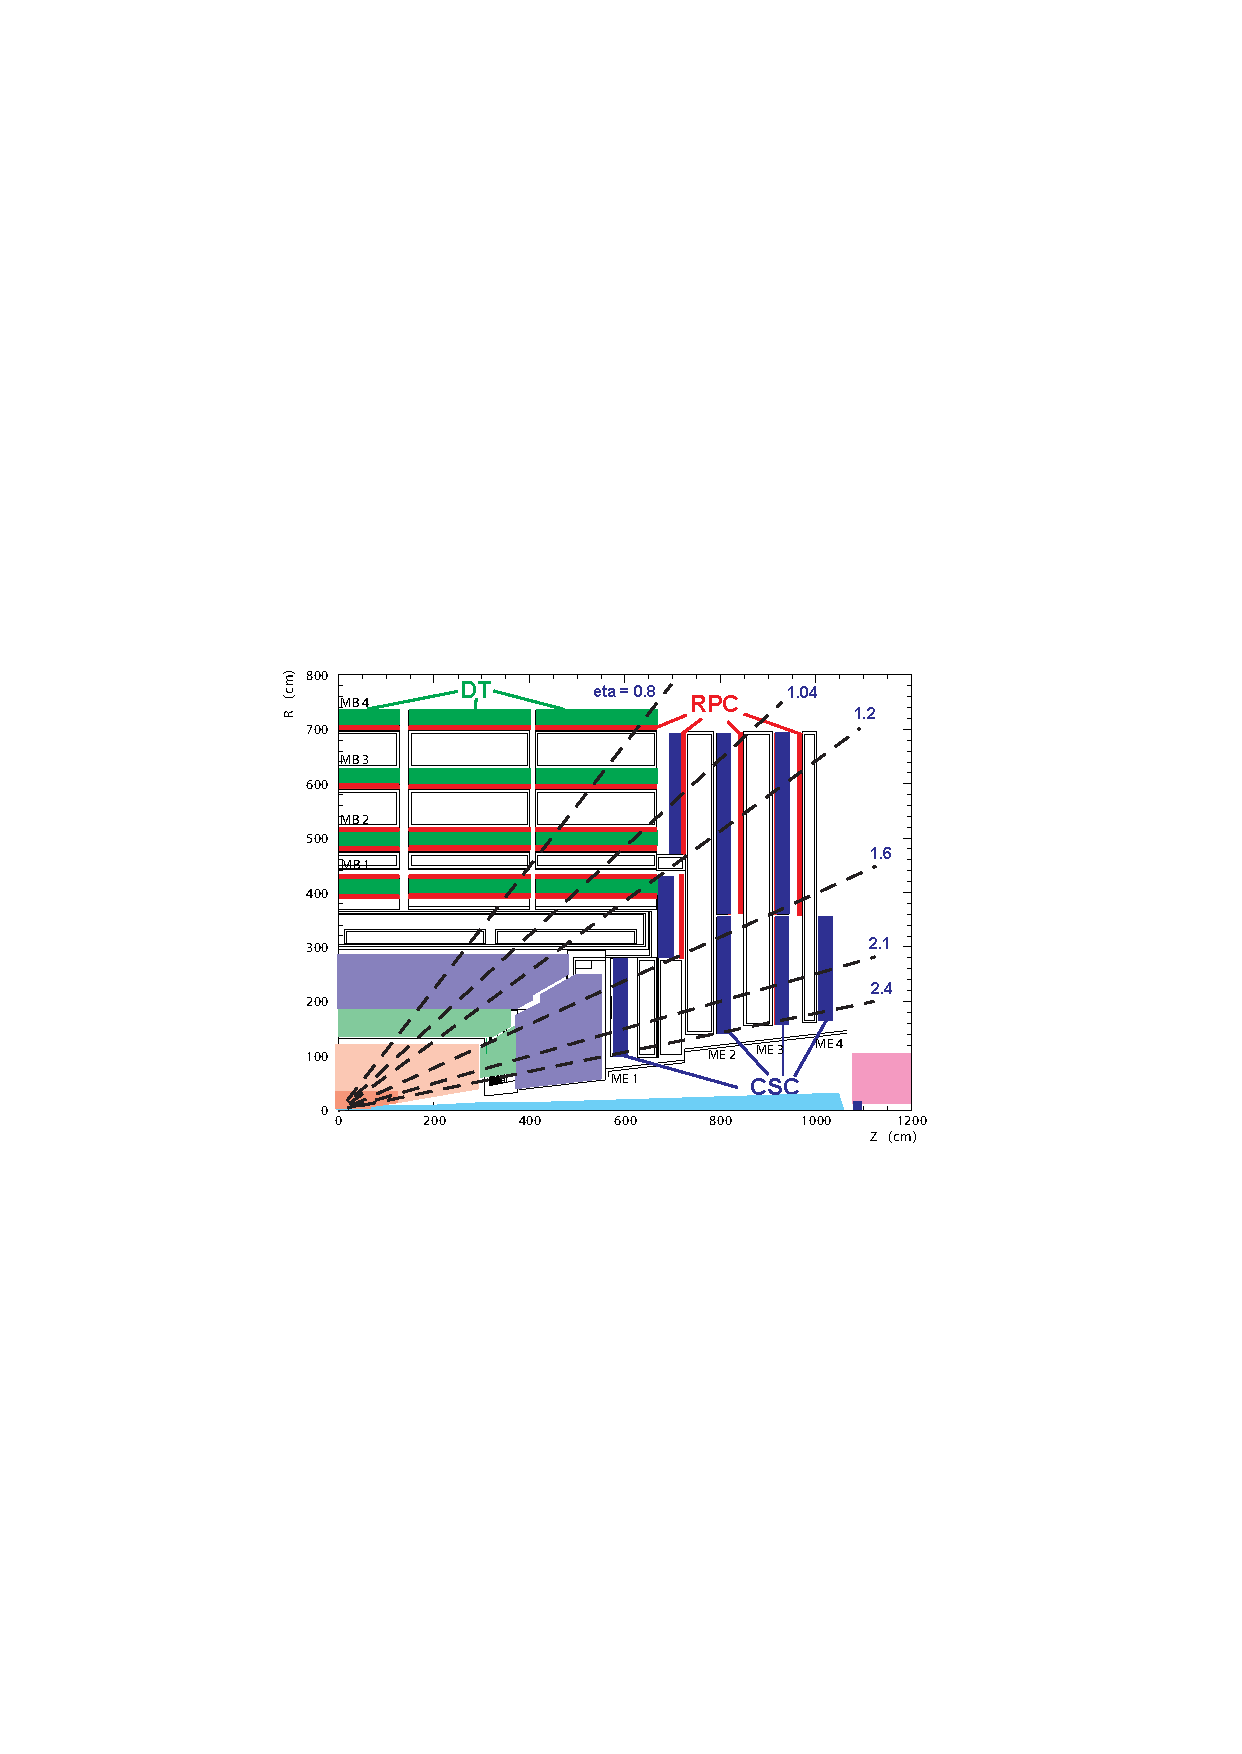
\includegraphics[width=0.95\textwidth]{\figpath/Chapter2/CMS_muon_system.pdf}
	\caption{Layout of the muon system with the three different detector technologies labeled.}
	\label{fig:CMS_muon_system}
\end{figure}

The DTs are divided into four stations named MB1 through MB4 (Muon Barrel), starting radially from the center of the detector outward.
The first three stations contain 12 chambers divided into three groups of four.
Two of the groups measure the $r-\phi$ coordinates of the muon while the third group measures the $z$ coordinate.
However, MB4 does not have a group of chambers which measured the $z$ coordinate.
The four stations contain 250 DTs in total with a collective 172000 sensitive wires, covering an $\eta$ range of \absetalt{1.2}.
The chambers themselves contain a gas mixture of 85\% Ar and 15\% CO\textsubscript{2} and have gold-plated, stainless steel anode wires with a diameter of 50\mum.
Within \absetalt{0.8}, the MB stations can reconstruct a high-\pt muon track with an efficiency greater than 95\%.
The global $r-\phi$ resolution is 100\mum.
Fig~\ref{fig:CMS_muon_system_DT} gives a transverse view of the DTs in one of the five wheels of CMS.

\begin{figure}[!hbt]
	\centering
	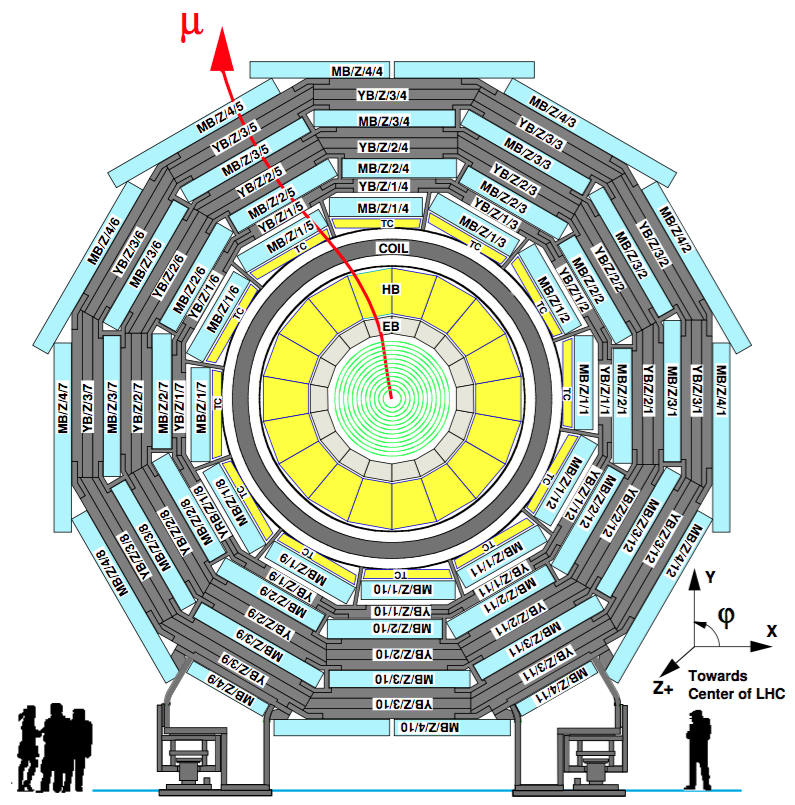
\includegraphics[width=0.95\textwidth]{\figpath/Chapter2/CMS_muon_system_DT}
	\caption{Transverse view of one of the five wheels of the CMS detector. The DTs and their layout can be clearly seen~\cite{Chatrchyan:2008aa}.}
	\label{fig:CMS_muon_system_DT}
\end{figure}

The CSCs are separated into four stations as well, names ME1 through ME4 (Muon Endcap), and cover \abseta{0.9}{2.4}.
ME1 has three groups of 72 CSC, ME2 and ME3 each have one group of 36 CSCs and one group of 72 CSCs, and ME4 has one group of 36 CSCs.
Thus each endcap contains 468 CSCs total.
Within a CSC the cathode strips are arranged radially in order to measure the $r-\phi$ coordinate of the muon.
The anode wires are then arranged perpendicular to the strips in order to measure the $\eta$ coordinate.
The cathode strips themselves are made of a fiberglass and epoxy material called FR4, which is coated with 36\mum of copper.
The anode wires are gold-plated tungsten with a diameter of 50\mum (the first group of ME1 uses 30\mum wires).
There are approximately 220000 cathode strip readout channels and 180000 anode wire readout channels in total.
Each CSC contains a gas mixture of 40\% Ar, 50\% CO\textsubscript{2}, and 10\% CF\textsubscript{4}.

The RPCs are meant to aid in triggering on muons.
They cover out to \absetalt{1.6} and can provide information to the trigger system much faster than the DTs or CSCs.
The time resolution for the RPCs is less than 3\unit{ns}, whereas the DTs and CSCs have a maximum drift time of 400\unit{ns} 60\unit{ns}, respectively.
With such a small time resolution, the RPCs can precisely identify the bunch crossing time of a muon candidate.
MB1 and MB2 have one internal and one external group of RPCs, relative to the DTs.
MB3 and MB4 each have two internal groups of RPCs.
This amounts to 480 RPCs for the barrel.
The endcap has 3 stations of RPCs, 144 chambers in total, arranged in concentric circle on the iron return yoke.
The RPCs are a type of parallel plate detector with a gas mixture of 96.2\% C\textsubscript{2}H\textsubscript{2}F\textsubscript{4}, 3.5\% C\textsubscript{4}H\textsubscript{10}, and 0.3\% SF\textsubscript{6}.

\subsection{Trigger}

In order to provide as many collisions as possible to the experiments, the LHC must operate at a high luminosity (see sec.~\ref{sec:LHC}).
At the proposed LHC center-of-mass energies the p-p collision cross section is about 100\unit{mb}.
This, combined with the luminosity, gives us a collision rate of approximately 1\unit{MHz}.
At this rate it would be impossible for the experiment to store and process all of the raw information coming from the detector.
Thus a trigger system is implemented to reduce this rate and keep only the most interesting, and hopefully relevant, events.
%Keeping events most likely to contain new physics
CMS has implemented a two-tiered trigger system~\cite{Khachatryan:2016bia}.
The first level (L1), composed of custom hardware processors, uses information from the calorimeters and muon detectors to select events at a rate of around 100\unit{kHz} within a time interval of less than 4\mus.
The second level, known as the high-level trigger (HLT), consists of a farm of processors running a version of the full event reconstruction software optimized for fast processing, and reduces the event rate to less than 1\unit{kHz} before data storage.

\begin{figure}[!hbt]
	\centering
	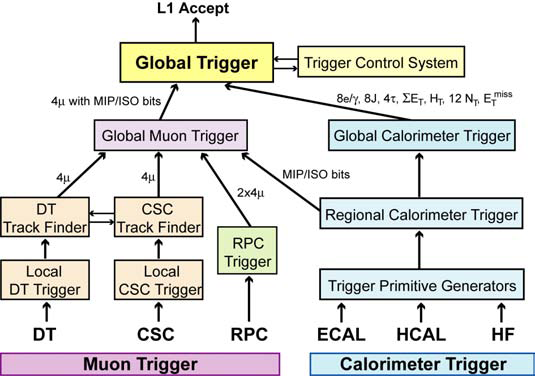
\includegraphics[width=0.95\textwidth]{\figpath/Chapter2/L1_architecture.png}
	\caption{The architecture of the L1 trigger system.}
	\label{fig:CMS_L1_architecture}
\end{figure}

The L1 trigger is is composed of custom built, programmable electronics including field programmable gate arrays (FPGAs), memory lookup tables (LUTs) and application specific integrated circuits (ASICs).
The components of this trigger system are arranged so that there can be local, regional, and global decision making (see fig.~\ref{fig:CMS_L1_architecture}).
Most of the sub-detectors send information to this trigger system, but due to the algorithmic complexity of track finding, the process would take too long if the tracker was included in the decision making process.
A new ``track trigger'' system is in the process of being developed, which would allow tracking information to be included in the L1 trigger decision making process.

The calorimeter side of the L1 trigger system starts with the Trigger Primitive Generators (TPG), which are constructed from energy deposits in the ECAL, HCAL, and HF.
These are then combined in the Regional Calorimeter Trigger (RCT), which groups the calorimeter towers into regions.
A region is defined as four towers for the barrel and endcap and one tower for the HF.
The regions are used to find photon and electron candidates, measure transverse energy sums ($\Sigma\ET$), and determine tau-jet vetoes.
The RCT also sends information to the Global Muon Trigger (GMT) about energy deposits to help determine if a muon candidate is isolated.
The information is then sent to the Global Calorimeter Trigger (GCT), which determines the jet candidates, providing up to four jets and four tau-jets from the central HCAL and four jets from the HF.
The GCT also calculates the \ET, \ETslash, and \HT, which is calculated as $\Sigma\ET$ for all jets above a certain threshold.

Each of the muon sub-detector's technologies (DT, CSC, and RPC) has a local trigger system.
The Regional Muon Trigger (RMT) takes the local trigger information from the DT and CSC and makes tracks using the DT and CSC Track Finders (DTTF and CSCTF).
In contrast, the RPCs are a form of dedicated trigger due to their small time resolution.
The Global Muon Trigger (GMT) combines the information from the RMT and RPCs to produce up to four muon candidates in each of the barrel and endcap regions.
The GMT also contains information about the \pt, charge, $\eta$, $\phi$, quality, MIP, and isolation of each of the muon candidates.

Finally, the Global Trigger (GT) combines the GCT and GMT information to decide whether or not to store the event; a decision which is called a Level-1 Accept (L1A).
The GT also makes use of information about the sub-detector readouts and DAQ systems from the Trigger Control System (TCS). The L1A is returned to the sub-detectors by the Timing, Trigger, and Control (TTC) system.
This entire process takes 3.2\mus, an equivalent of $\mathcal{O}(100)$ bunch crossings, which means that the data must be pipelined in order to synchronize the steps in the trigger system.
Meanwhile, the high resolution data used for offline analysis is stored in memory. In 2012, the L1 Trigger rate was as high as 100\unit{kHz} with a dead time of only 3\%~\cite{Brooke:2013hnf}.

After the L1A decision, the High Level Trigger (HLT), a farm of more than 13000 central processing units (CPUs), further analyzes the events. The HLT 
system uses a form of the full offline reconstruction algorithms described in chapter~\ref{ch:event_reconstruction}, but also includes several optimizations to make the process faster. This is needed because, in contrast to offline processing, the HLT is limited by the number of events that can be stored in the pipeline. These optimizations include making the fasted algorithm run first, skipping a trigger path after the first failing quality filter, and considering smaller regions of the detector based on the L1 candidates. The menu of triggers to be run changes as the LHC and MC conditions change, even while CMS is operational. In 2012, the HLT had an output rate of 100\unit{kHz} and took 200\unit{ms} per event, $\mathcal{O}(100)$ times faster than the offline reconstruction~\cite{Trocino:2014jya}. Events that pass the HLT are then sorted into primary datasets (PDs) according to the passed triggers with as little overlap as possible.

\subsection{Luminosity Measurement}

Besides measuring the kinematics of each of the particles traversing the detector, CMS must also measure the instantaneous luminosity delivered by the LHC.
Both the pixel detector (section~\ref{sec:tracker_and_pixel}) and the HF (section~\ref{sec:hadron_calorimeter}) are able to measure the luminosity to varying degrees of accuracy.

The pixel detector has a very small granularity, which means that any given pixel is activated by at most one track per bunch crossing.
We can then create cluster by grouping nearby activated pixels, with the typical cluster containing an average of 5 pixels.
A minimum bias event typically creates 200 clusters~\cite{CMS-PAS-LUM-12-001}.
Even for events with 100 pileup interactions, a number significantly higher than was reached in 2012, the total pixel detector occupancy could be as low as 0.1\%.
This means that the number of pixel hits should scale linearly with the number of interactions per bunch crossing, which is shown in equation~\ref{eq:pixel_luminosity_measurement}~\cite{CMS-PAS-LUM-13-001}.

\begin{equation}
\mathcal{L}=\frac{\nu\average{n}}{\sigma_{vis}}
\label{eq:pixel_luminosity_measurement}
\end{equation}

Here the luminosity, $\mathcal{L}$, is proportional to average number of pixel clusters, \average{n}.
The other parameters are the LHC revolution frequency, $\nu=11246\unit{Hz}$ and the visible cross section, $\sigma_\text{vis}$, as calibrated by a Van der Meer scan~\cite{Balagura:2011yw}.
In 2012 this technique was used to measure the total integrated luminosity with a systematic uncertainty of 2.6\%.

Another method to measure the luminosity makes use of the HF, but due to some sever limitations in its accuracy, this measurement is only used as a cross-check for the pixel counting method.
What makes the HF suitable for this type of measurement is that it can safely be run during unstable beams~\cite{CMS-PAS-LUM-13-001}.
The average transverse energy per tower can be directly related to the luminosity or the average fraction of empty towers can be related to the mean number of interactions per crossing, which is more of in indirect measurement.
The benefit of using the HF is that it can make an online determination of the luminosity within 1\unit{s} to an accuracy of 1\%.
One downside is that even in 2012 the levels of pileup made the luminosity relationship non-linear.
Additionally, the calibration of this measurement can change due to drifts in the gains of the HF PMTs~\cite{Pedro2014}.
%!TEX root = ../TAMUTemplate.tex
%%%%%%%%%%%%%%%%%%%%%%%%%%%%%%%%%%%%%%%%%%%%%%%%%%%
%
%  New template code for TAMU Theses and Dissertations starting Fall 2016.
%
%  Author: Sean Zachary Roberson
%	 Version 3.16.09
%  Last updated 9/12/2016
%
%%%%%%%%%%%%%%%%%%%%%%%%%%%%%%%%%%%%%%%%%%%%%%%%%%%
%%%%%%%%%%%%%%%%%%%%%%%%%%%%%%%%%%%%%%%%%%%%%%%%%%%%%%%%%%%%%%%%%%%%%%
%%                           SECTION IV
%%%%%%%%%%%%%%%%%%%%%%%%%%%%%%%%%%%%%%%%%%%%%%%%%%%%%%%%%%%%%%%%%%%%%



\chapter{\uppercase {Event Reconstruction}}
\label{ch:event_reconstruction}

The CMS detector is designed to identify the various particle species which travel through it after a proton-proton collision.
As discussed in chapter~\ref{ch:LHC_CMS}, the sub-detector technologies were chosen so that particles could be identified by where they deposite their energy as well as how their trajectories change in a magnetic field.
Fig~\ref{fig:particle_flow} shows how various types of particles interact with the CMS detector.
All of the charged particles (\ie electrons, muons, and charged hadrons) will deposit some energy in the tracker, while neutral particles (\ie photons and neutral hadrons) will not.
Electrons and photons will deposit all of their energy inside of the ECAL while hadrons, both charged and neutral, will deposit most of their energy in the HCAL.
Muons are the only visible particle which will be able to travel to the muon chambers.
Neutrinos will pass through all layers of the detector unseen and their presence must be infered by missing transverse energy (\MET or \ETslash); the idea being that if the sum of the transverse momentum is not conserved, then that missing momentum must correspond to at least one unseen particle.

\begin{figure}[!hbt]
	\centering
	\includegraphics[width=0.95\textwidth]{\figpath/Chapter3/ParticleFlow}
	\caption{Cross-sectional view of the CMS detector with all of the sub-detectors labeled.The colored lines correspond to different particle species, which interact with different pieces of the detector and may or may not be bent by the magnetic field.}
	\label{fig:particle_flow}
\end{figure}

The process of translating abstract detector objects to physical particles takes several steps within the CMS software framework (CMSSW).
The first of this process is local reconstruction, where the various subsystems of each sub-detector create what are called reconstucted hits, or RecHits for short.
RecHits in the tracker contain information about the position of energy clusters (groups of contiguous strips or pixels which contain a signal) as well as energy deposition information which aids in particle identification.
The muon RecHits ostensibly contain information about the position of the signal.
However, the RecHits from the DTs and CSCs can be combined to form three-dimensional track segments, which also provide directional information.
The ECAL and HCAL RecHits contain information about the energy deposited, the position of those deposits, and the time at which they occured.

The next step is to process this information in a global manner, where the subsystems within each sub-detector are combined.
Pattern recongnition algorithms are run on the tracker RecHits to reconstruct the path that the particles take through the sub-detector (a.k.a tracks).
The ECAL and HCAL RecHits within a tower are summed to form ``CaloTowers'' which have a projective $\eta-\varphi$ geometry.
The muon system creates ``standalone'' muons by associating RecHits and track segments with compatible radial trajectories.
This process takes into account the bending a muon undergoes before reaching and within the muon system due to the magnetic field.

At this point, all of the reconstuction information is combined to form particles that can be used for physics analysis.
The process of reconstucting and classifying every stable particle is called Particle Flow (PF) and will be discussed further in chapter~\ref{sec:particle_flow}.
This analysis focuses on electrons, muons, jets, b-jets, and \ETslash, the reconstuction of which will be described in the following sections.
Additional information about the reconstruction process beyond the scope of this thesis can be found in~\cite{TDR-software}.

\section{Tracks and Vetices}
\label{sec:tracks_and_vertices}

While CMS analyses cover a wide range of final states, a majority of them will include jets in some fashion, including this one.
It's important that the particle flow algorithm identify and measure each particle inside a jet in order to improve the jet energy response and resolution.
Section~\ref{sec:jets} will cover the reconstruction and properties of jets in more detail, but it is important to note that two thirds of the constituents inside of a jet are charged particles.
This motivates the need for excellent tracking capabilities.
Tracks are created from the RecHits using the Combinatorial Track Finder (CTF) algorithm, which is an iterative process~\cite{TrackingJINST}.
This process seeks to find the appropriate balance between high reconstruction efficiency and low fake rate (see fig~\ref{fig:efficiency_vs_fake_rate})~\cite{CMS-PAS-PFT-09-001}.

\begin{figure}[!hbt]
	\centering
	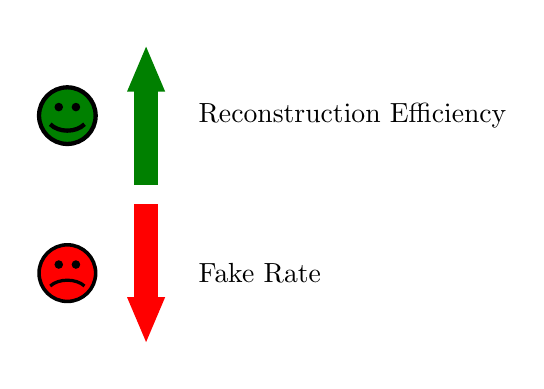
\begin{tikzpicture}[node distance = 2cm, auto]
		\tikzstyle{myarrows}=[line width=1mm,-triangle 45,postaction={draw, line width=3mm, shorten >=4mm, -}]
	
		\node (up) at (0,2) {};
		\node (center) at (0,0) {};
		\node (down) at (0,-2) {};
	
		\draw[myarrows,green!50!black] (center) -- node[right,black,xshift=5mm] {Reconstruction Efficiency} ++ (up);
		\draw[myarrows,red] (center) -- node[right,black,xshift=5mm] {Fake Rate} ++ (down);
	
		\node (smiley) at (-1,1)  {\Smiley[3][green!50!black]};
		\node (sadey)  at (-1,-1) {\Sadey[3][red]};
	\end{tikzpicture}
	\caption{A diagram showing the goals of the iterative tracking process.}
	\label{fig:efficiency_vs_fake_rate}
\end{figure}

The track finding proceedure begins by finding track seeds using only a few hits and very tight criteria.
A track is built by extrpolating from the trajectory of the seed and adding new hits that match this trajectory, keeping in mind that charged particles will bend in the presence of the magnetic field.
The tight requirements on this first step lead to a moderate tracking efficiency, vanishingly small fake rate.
After a track is found, all of the hits are used in a fit to determine the track parameters (i.e. \pt, $\chi^{2}$, etc.), which are then used to judge the quality of the track.
If a track doesn't meet certain quality requirments, it isn't kept.
The hits which are unambiguaously assigned to the tracks found are removed from consideration in the next iteration and their tracks saved for later use.

\begin{figure}[!hbt]
	\centering
	\includegraphics[width=0.75\textwidth]{\figpath/Chapter3/RadiusOfCurvature}
	\caption{Schematic view of a particle track with hits labeled.}
	\label{fig:radius_of_curvature}
\end{figure}

In each subsequent iteration the track seeding criteria is loosened and the same proceedure occurs.
The looser seeding requirments boosts the tracking efficiency, while the removal of the hits from the previous iteration keeps the fake rate low due to the reduced combinatorics.
The specific seeding criteria for each iteration can be found in table~\ref{tab:track_seeding}.
After three iterations 90\% of charged hadron tracks are reconstructed and 99.5\% of muons in the tracker acceptance are found.
Subsequent iterations loosen the constraints on the origin vertex, which allows for the reconstructions of tracks associated with a secondary vertex (i.e. $\gamma\rightarrow$\Pep\Pem~conversions, long-lived particles, nuclear interactions in the tracker material).
Tracks meeting this set of criteria can be reconstructed with as little as three hits, a \pt as low as 150\mev, and a vertex  more than 50\unit{cm} away from the beam axis.
Nevertheless, the fake rate is still kept on the order of 1\%~\cite{CMS-PAS-PFT-09-001}.

\begin{table}[htbp]
	\caption{The seed and track criteria used in each iteration during the 2012 run. The seed types, pair and triplet, indicate if two or three RecHits are used, respectively. The $\sigma$ in the $z_0$ criteria indicated the length of the beam spot in the $z$-direction as determined by a Gaussian fit~\cite{Tracking2012}.}
	\centering
    \begin{tabular}{llllll}
		\hline
		step  & seed type & seed subdetectors & \pt $[\GeVcns]$ & $d_0$ [cm] & $|z_0|$ \\
		\hline
		0     & triplet   & pixel             & ${>}0.6$     & ${<}0.02$  & ${<}4.0\sigma$ \\
		1     & triplet   & pixel             & ${>}0.2$     & ${<}0.02$  & ${<}4.0\sigma$ \\
		2     & pair      & pixel             & ${>}0.6$     & ${<}0.015$ & ${<}0.09\cm$ \\
		3     & triplet   & pixel             & ${>}0.3$     & ${<}1.5$   & ${<}2.5\sigma$ \\
		4     & triplet   & pixel/TIB/TID/TEC & ${>}0.5$--0.6 & ${<}1.5$   & ${<}10.0\cm$ \\
		5     & pair      & TIB/TID/TEC       & ${>}0.6$     & ${<}2.0$   & ${<}10.0\cm$ \\
		6     & pair      & TOB/TEC           & ${>}0.6$     & ${<}2.0$   & ${<}30.0\cm$ \\
		\hline
    \end{tabular}
	\label{tab:track_seeding}
\end{table}

The tracks found will have a helical shape of with a given radius of curvature as in fig~\ref{fig:radius_of_curvature}.
The softest, low \pt particle trajectories can form small rings, while the higher \pt particles will be bent less.
The momentum of each track can be extracted from the radius of curviture (R), given by a circular fit to the track, the magnetic field strength, as well as $\eta$ and $\varphi$ of the track at the interaction point\footnote{The $\eta$ of the track is determined as if the interaction point was at the center of the detector.}.
The following system of equations can be used to determine the particles 3-momenta at the interaction point:
\begin{equation}
	\begin{aligned}
		p_{x}&=p_{T}\cos\varphi\\
		p_{y}&=p_{T}\sin\varphi\\
		p_{z}&=p_{T}\sinh\eta\\
		p_{T}&=0.3\cdot{B}\cdot{R}
	\end{aligned}
\end{equation}

After the collection of high purity tracks is created, CMS uses these to reconstruct the location of the vertices where proton-proton interactions occured~\cite{TrackingJINST}.
The vertex finding algorithm is agnostic to whether or not the verteces come from the main hard scatter vertex of interest or any of the pileup vertices from additional proton-proton interactions.



\section{Particle Flow}
\label{sec:particle_flow}

The CMS experiment has decided to use a holistic approach to reconstucting the event produced by a proton-proton collision.
The particle flow (PF) event reconstuction algorithm uses information from all of the sub-detectors in order to reconstruct (direction and energy) and identify as accurately as possible each individual particle in the event as descibed in the first part of this chapter~\cite{CMS-PAS-PFT-09-001}.
The CMS detector, with its extremely granular sub-detectors and high magnetic field, is ideally suited for a particle flow approach.
With the current algorithm, charged-particle tracks out to \absetalt{2.6} can be reconstucted even with a \pt as low as 150\mev, all while maintaining a high reconstruction efficiency and low fake rate.
Photons can be separated from charged-particle energy deposits even in high multiplicity environments like jets.
Although the HCAL is 25 times coarser than the ECAL, the energy resolution is enough to detect neutral hadrons as an energy excess above that deposited by charged hadrons.
Fig~\ref{fig:particle_flow} show, in graphical terms, how the reconstruction algorithm can classify a particle based on the sub-detectors with which it interacts.
The PF algorithm's performance and commisioning is discussed in~\cite{CMS-PAS-PFT-10-002,CMS-PAS-PFT-10-003} using early CMS data and again using newer data and a slightly updated algorithm in~\cite{Beaudette:2014cea}.
All three of these papers indicate a significant improvement in particle identification and object reconstruction over simpler approaches.

The inputs to the PF algorithm come from the local reco products, RecHits, as described at the start of chapter~\ref{ch:event_reconstruction}. More specifically the RecHits are turned into either tracks or energy clusters, which are then used by the algorithm. The tracks may come from the tracker, as described in section~\ref{sec:tracks_and_vertices}, or from the muon system. The clusters are created by the calorimeter RecHits and are treated slightly different than the CaloTowers previously discussed. A local energy maxima









The output of the PF algorithm is a list of particles known as ``PF candidates,'' which are used to build the higher level objects that physicists analyze, such as jets, taus, and \ETmiss. Other quantities that can be determined from a particle level reconstruction algorithm are the charged lepton isolation and the likelihood that a jet was initiated by a B hadron.





\begin{figure}[!hbt]
	\centering
	\begin{subfigure}[t]{0.53\textwidth}
		\includegraphics[width=\textwidth,angle=90]{\figpath/Chapter3/PFT-09-001_001_a.pdf}
		\caption{An $(x,y)$ view of the detector.}
		\label{fig:PF_linking_a}
	\end{subfigure}

	\begin{subfigure}[t]{0.4655\textwidth}
		\includegraphics[width=\textwidth]{\figpath/Chapter3/PFT-09-001_001_b.pdf}
		\caption{An $(\eta,\varphi)$ view of the ECAL.}
		\label{fig:PF_linking_b}
	\end{subfigure}
	\begin{subfigure}[t]{0.4655\textwidth}
		\includegraphics[width=\textwidth]{\figpath/Chapter3/PFT-09-001_001_c.pdf}
		\caption{An $(\eta,\varphi)$ view of the HCAL.}
		\label{fig:PF_linking_c}
	\end{subfigure}
	\caption{These three figures show a representation of how the PF algorithm sees a hadronic jet. (a) An $(x,y)$ view of the detector with elements from the tracker, ECAL, and HCAL shown. The ECAL and HCAL surfaces shown in (b) and (c) are represented by the concentric circles centered around the interaction point in (a). (b) shows the energy clusters from the \PKzL, \Pgpm, and the two photons from the \Pgpz decay. While the \Pgpp doesn't deposit any energy in the ECAL, it does show up as a cluster in the HCAL along with the \Pgpm (c). The tracks from these charged particles show up as vertical lines in the $(\eta,\varphi)$ plane, but as curved lines in the $(x,y)$ plane. The cluster positions are represented by dots, the simulated particles by dashed lines, and the position at which the particles impact the calorimeter surfaces by the open markers~\cite{CMS-PAS-PFT-09-001}.}
\end{figure}

\clearpage











In longer papers, the particle-flow algorithm can be described in more detail:

The global event reconstruction (also called particle-flow event reconstruction~\cite{CMS-PAS-PFT-09-001,CMS-PAS-PFT-10-001}) consists of reconstructing and identifying each individual particle with an optimized combination of all subdetector information.
In this process, the identification of the particle type (photon, electron, muon, charged hadron, neutral hadron) plays an important role in the determination of the particle direction and energy.
Photons (\eg coming from \Pgpz\ decays or from electron bremsstrahlung) are identified as ECAL energy clusters not linked to the extrapolation of any charged particle trajectory to the ECAL.
Electrons (\eg coming from photon conversions in the tracker material or from \cPqb-hadron semileptonic decays) are identified as a primary charged particle track and potentially many ECAL energy clusters corresponding to this track extrapolation to the ECAL and to possible bremsstrahlung photons emitted along the way through the tracker material.
Muons (\eg from \cPqb-hadron semileptonic decays) are identified as a track in the central tracker consistent with either a track or several hits in the muon system, associated with an energy deficit in the calorimeters.
Charged hadrons are identified as charged particle tracks neither identified as electrons, nor as muons.
Finally, neutral hadrons are identified as HCAL energy clusters not linked to any charged hadron trajectory, or as ECAL and HCAL energy excesses with respect to the expected charged hadron energy deposit.

The energy of photons is directly obtained from the ECAL measurement, corrected for zero-suppression effects.
The energy of electrons is determined from a combination of the track momentum at the main interaction vertex, the corresponding ECAL cluster energy, and the energy sum of all bremsstrahlung photons attached to the track.
The energy of muons is obtained from the corresponding track momentum.
The energy of charged hadrons is determined from a combination of the track momentum and the corresponding ECAL and HCAL energy, corrected for zero-suppression effects and for the response function of the calorimeters to hadronic showers.
Finally, the energy of neutral hadrons is obtained from the corresponding corrected ECAL and HCAL energy.


\section{Electrons}

The electron momentum is estimated by combining the energy measurement in the ECAL with the momentum measurement in the tracker.The momentum resolution for electrons with $\pt \approx 45\GeV$ from $\Z \rightarrow \Pe \Pe$ decays ranges from 1.7\% for nonshowering electrons in the barrel region to 4.5\% for showering electrons in the endcaps~\cite{Khachatryan:2015hwa}.

The dielectron mass resolution for $\Z \rightarrow \Pe \Pe$ decays when both electrons are in the ECAL barrel is 1.9\%, and is 2.9\% when both electrons are in the endcaps. The electron momenta are estimated by combining energy measurements in the ECAL with momentum measurements in the tracker~\cite{Khachatryan:2015hwa}. 

\section{Muons}

\section{Jets}
\label{sec:jets}

When combining information from the entire detector, the jet energy resolution amounts typically to 15\% at 10\GeV, 8\% at 100\GeV, and 4\% at 1\TeV, to be compared to about 40\%, 12\%, and 5\% obtained when the ECAL and HCAL calorimeters alone are used.


Traditional calorimetric jets are reconstructed offline from the energy deposits in the calorimeter towers, clustered by the anti-$k_\mathrm{t}$ algorithm~\cite{Cacciari:2008gp, Cacciari:2011ma} with a size parameter of 0.4. In this process, the contribution from each calorimeter tower is assigned a momentum, the absolute value and the direction of which are given by the energy measured in the tower, and the coordinates of the tower. The raw jet energy is obtained from the sum of the tower energies, and the raw jet momentum by the vectorial sum of the tower momenta, which results in a nonzero jet mass. The raw jet energies are then corrected to establish a relative uniform response of the calorimeter in $\eta$ and a calibrated absolute response in transverse momentum \pt. 

 The particle-flow algorithm can be described in short form as:

The particle-flow event algorithm reconstructs and identifies each individual particle with an optimized combination of information from the various elements of the CMS detector. The energy of photons is directly obtained from the ECAL measurement, corrected for zero-suppression effects. The energy of electrons is determined from a combination of the electron momentum at the primary interaction vertex as determined by the tracker, the energy of the corresponding ECAL cluster, and the energy sum of all bremsstrahlung photons spatially compatible with originating from the electron track. The energy of muons is obtained from the curvature of the corresponding track. The energy of charged hadrons is determined from a combination of their momentum measured in the tracker and the matching ECAL and HCAL energy deposits, corrected for zero-suppression effects and for the response function of the calorimeters to hadronic showers. Finally, the energy of neutral hadrons is obtained from the corresponding corrected ECAL and HCAL energy.

to be followed by these other lines, after mentioning the anti-\kt algorithm:

Jet momentum is determined as the vectorial sum of all particle momenta in the jet, and is found from simulation to be within 5 to 10\% of the true momentum over the whole \pt spectrum and detector acceptance. An offset correction is applied to jet energies to take into account the contribution from additional proton-proton interactions within the same or nearby bunch crossings. Jet energy corrections are derived from simulation, and are confirmed with in situ measurements of the energy balance in dijet and photon + jet events. Additional selection criteria are applied to each event to remove spurious jet-like features originating from isolated noise patterns in certain HCAL regions.

In some papers, you would want to add some performance numbers:

The jet energy resolution amounts typically to 15\% at 10\GeV, 8\% at 100\GeV, and 4\% at 1\TeV, to be compared to about 40\%, 12\%, and 5\% obtained when the calorimeters alone are used for jet clustering.

For each event, hadronic jets are clustered from these reconstructed particles with the infrared and collinear safe anti-\kt algorithm, operated with a size parameter $R$ of 0.4. The jet momentum is determined as the vectorial sum of all particle momenta in this jet, and is found in the simulation to be within 5 to 10\% of the true momentum over the whole \pt spectrum and detector acceptance. Jet energy corrections are derived from the simulation, and are confirmed with in situ measurements with the energy balance of dijet and photon + jet events~\cite{Chatrchyan:2011ds}. The jet energy resolution amounts typically to 15\% at 10\GeV, 8\% at 100\GeV, and 4\% at 1\TeV, to be compared to about 40\%, 12\%, and 5\% obtained when the calorimeters alone are used for jet clustering. 

\section{Missing Transverse Energy}


\section{Event Generation}

\section{Detector Simulation}
%%!TEX root = ../TAMUTemplate.tex
%%%%%%%%%%%%%%%%%%%%%%%%%%%%%%%%%%%%%%%%%%%%%%%%%%%
%
%  New template code for TAMU Theses and Dissertations starting Fall 2016.
%
%  Author: Sean Zachary Roberson
%    Version 3.16.09
%  Last updated 9/12/2016
%
%%%%%%%%%%%%%%%%%%%%%%%%%%%%%%%%%%%%%%%%%%%%%%%%%%%
%%%%%%%%%%%%%%%%%%%%%%%%%%%%%%%%%%%%%%%%%%%%%%%%%%%%%%%%%%%%%%%%%%%%%%
%%                           SECTION IV
%%%%%%%%%%%%%%%%%%%%%%%%%%%%%%%%%%%%%%%%%%%%%%%%%%%%%%%%%%%%%%%%%%%%%



\chapter{\texorpdfstring{\uppercase {Event Reconstruction}}{Event Reconstruction}}
\label{ch:event_reconstruction}

The CMS detector is designed to identify the various particle species which travel through it after a proton-proton collision.
As discussed in chapter~\ref{ch:LHC_CMS}, the sub-detector technologies were chosen so that particles could be identified by where they deposit their energy as well as how their trajectories change in a magnetic field.
Fig.~\ref{fig:particle_flow} shows how various types of particles interact with the CMS detector.
All of the charged particles (\ie electrons, muons, and charged hadrons) will deposit some energy in the tracker, while neutral particles (\ie photons and neutral hadrons) will not.
Electrons and photons will deposit all of their energy inside of the ECAL while hadrons, both charged and neutral, will deposit most of their energy in the HCAL.
Muons are the only visible particle which will be able to travel to the muon chambers.
Neutrinos will pass through all layers of the detector unseen and their presence must be inferred by missing transverse energy (\MET or \ETslash); the idea being that if the sum of the transverse momentum is not conserved, then that missing momentum must correspond to at least one unseen particle.

\begin{figure}[!hbt]
    \centering
    \includegraphics[width=0.95\textwidth]{\figpath/Chapter4/ParticleFlow}
    \caption{Cross-sectional view of the CMS detector with all of the sub-detectors labeled.The colored lines correspond to different particle species, which interact with different pieces of the detector and may or may not be bent by the magnetic field.}
    \label{fig:particle_flow}
\end{figure}
t
The process of translating abstract detector objects to physical particles takes several steps within the CMS software framework (CMSSW).
The first of this process is local reconstruction, where the various subsystems of each sub-detector create what are called reconstructed hits, or RecHits for short.
RecHits in the tracker contain information about the position of energy clusters (groups of contiguous strips or pixels which contain a signal) as well as energy deposition information which aids in particle identification.
The muon RecHits ostensibly contain information about the position of the signal.
However, the RecHits from the DTs and CSCs can be combined to form three-dimensional track segments, which also provide directional information.
The ECAL and HCAL RecHits contain information about the energy deposited, the position of those deposits, and the time at which they occurred.

The next step is to process this information in a global manner, where the subsystems within each sub-detector are combined.
Pattern recognition algorithms are run on the tracker RecHits to reconstruct the path that the particles take through the sub-detector (a.k.a tracks).
The ECAL and HCAL RecHits within a tower are summed to form ``CaloTowers'' which have a projective $\eta-\varphi$ geometry.
The muon system creates ``standalone'' muons by associating RecHits and track segments with compatible radial trajectories.
This process takes into account the bending a muon undergoes before reaching and within the muon system due to the magnetic field.

At this point, all of the reconstruction information is combined to form particles that can be used for physics analysis.
The process of reconstructing and classifying every stable particle is called Particle Flow (PF) and will be discussed further in chapter~\ref{sec:particle_flow}.
This analysis focuses on electrons, muons, jets, b-jets, and \ETslash, the reconstruction of which will be described in the following sections.
Additional information about the reconstruction process beyond the scope of this thesis can be found in~\cite{TDR-software}.

\section{Tracks and Vertices}
\label{sec:tracks_and_vertices}

While CMS analyses cover a wide range of final states, a majority of them will include jets in some fashion, including this one.
It's important that the particle flow algorithm identify and measure each particle inside a jet in order to improve the jet energy response and resolution.
Section~\ref{sec:jets} will cover the reconstruction and properties of jets in more detail, but it is important to note that two thirds of the constituents inside of a jet are charged particles.
This motivates the need for excellent tracking capabilities.
Tracks are created from the RecHits using the Combinatorial Track Finder (CTF) algorithm, which is an iterative process~\cite{TRK-11-001}.
This process seeks to find the appropriate balance between high reconstruction efficiency and low fake rate (see fig.~\ref{fig:efficiency_vs_fake_rate})~\cite{CMS-PAS-PFT-09-001}.

\begin{figure}[!hbt]
    \centering
    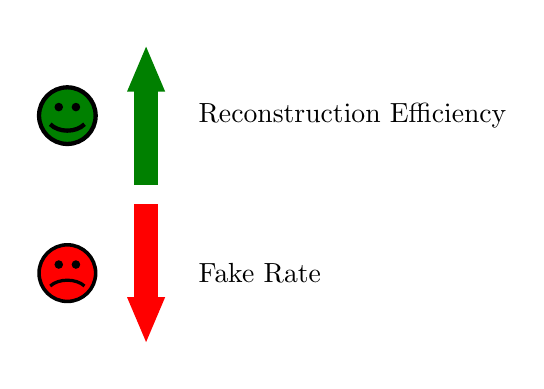
\begin{tikzpicture}[node distance = 2cm, auto]
        \tikzstyle{myarrows}=[line width=1mm,-triangle 45,postaction={draw, line width=3mm, shorten >=4mm, -}]
    
        \node (up) at (0,2) {};
        \node (center) at (0,0) {};
        \node (down) at (0,-2) {};
    
        \draw[myarrows,green!50!black] (center) -- node[right,black,xshift=5mm] {Reconstruction Efficiency} ++ (up);
        \draw[myarrows,red] (center) -- node[right,black,xshift=5mm] {Fake Rate} ++ (down);
    
        \node (smiley) at (-1,1)  {\Smiley[3][green!50!black]};
        \node (sadey)  at (-1,-1) {\Sadey[3][red]};
    \end{tikzpicture}
    \caption{A diagram showing the goals of the iterative tracking process.}
    \label{fig:efficiency_vs_fake_rate}
\end{figure}

The track finding procedure begins by finding track seeds using only a few hits and very tight criteria.
A track is built by extrapolating from the trajectory of the seed and adding new hits that match this trajectory, keeping in mind that charged particles will bend in the presence of the magnetic field.
The tight requirements on this first step lead to a moderate tracking efficiency and a vanishingly small fake rate.
After a track is found, all of the hits are used in a fit to determine the track parameters (i.e. \pt, $\chi^{2}$, etc.), which are then used to judge the quality of the track.
If a track doesn't meet certain quality requirements on the \pt, the transverse impact parameter $d_{0}$, and the longitudinal impact parameter $d_{z}$, it isn't kept.
Additionally, a trajectory cleaning step to remove duplicate tracks is applied to each iteration and to the final track collection.
A duplicate track can form either from different seeds or from the same seed which forms two very similar tracks.
If a pair of any two tracks share more than 19\% of hits as determined by equation~\ref{eq:trajectory_cleaning}, where $N^{hits}_{1}$ and $N^{hits}_{2}$ are the number of hits used in forming the tracks and 19\% is an empirically determined value, then the track with the fewest number of hits or the largest $\chi^{2}$ is removed.
The hits which are unambiguously assigned to the tracks are removed from consideration in the next iteration and their tracks saved for later use.

\begin{equation}
\label{eq:trajectory_cleaning}
f_{shared}=\frac{M^{hits}_{shared}}{min\left(N^{hits}_{1},N^{hits}_{2}\right)}
\end{equation}

\begin{figure}[!hbt]
    \centering
    \includegraphics[width=0.75\textwidth]{\figpath/Chapter4/RadiusOfCurvature}
    \caption{Schematic view of a particle track with hits labeled.}
    \label{fig:radius_of_curvature}
\end{figure}

In each subsequent iteration the track seeding criteria is loosened and the same procedure occurs.
The looser seeding requirements boosts the tracking efficiency, while the removal of the hits from the previous iteration keeps the fake rate low due to the reduced combinatorics.
The specific seeding criteria for each iteration can also be found in table~\ref{tab:track_seeding}.
After three iterations, 90\% of charged hadron tracks within jets are reconstructed and 99.5\% of muons in the tracker acceptance are found.
Subsequent iterations loosen the constraints on the origin vertex, which allows for the reconstructions of tracks associated with a secondary vertex (i.e. $\gamma\rightarrow$\Pep\Pem~conversions, long-lived particles, nuclear interactions in the tracker material).
Tracks meeting this set of criteria can be reconstructed with as little as three hits, a \pt as low as 150\mev, and a vertex  more than 50\unit{cm} away from the beam axis.
Nevertheless, the fake rate is still kept on the order of 1\%~\cite{CMS-PAS-PFT-09-001}.

\begin{table}[htbp]
    \caption{The seed criteria used in each iteration during the 2012 run. The seed types, pair and triplet, indicate if two or three RecHits are used, respectively. The $\sigma$ in the $z_0$ criteria indicated the length of the beam spot in the $z$-direction as determined by a Gaussian fit~\cite{Tracking2012}.}
    \centering
    \begin{tabular}{llllll}
        \hline
        step  & seed type & seed sub-detectors & \pt $[\GeVcns]$ & $d_0$ [cm] & $|z_0|$ \\
        \hline
        0     & triplet   & pixel             & ${>}0.6$     & ${<}0.02$  & ${<}4.0\sigma$ \\
        1     & triplet   & pixel             & ${>}0.2$     & ${<}0.02$  & ${<}4.0\sigma$ \\
        2     & pair      & pixel             & ${>}0.6$     & ${<}0.015$ & ${<}0.09\cm$ \\
        3     & triplet   & pixel             & ${>}0.3$     & ${<}1.5$   & ${<}2.5\sigma$ \\
        4     & triplet   & pixel/TIB/TID/TEC & ${>}0.5$--0.6 & ${<}1.5$   & ${<}10.0\cm$ \\
        5     & pair      & TIB/TID/TEC       & ${>}0.6$     & ${<}2.0$   & ${<}10.0\cm$ \\
        6     & pair      & TOB/TEC           & ${>}0.6$     & ${<}2.0$   & ${<}30.0\cm$ \\
        \hline
    \end{tabular}
    \label{tab:track_seeding}
\end{table}

The tracks found will have a helical shape of with a given radius of curvature as in fig.~\ref{fig:radius_of_curvature}.
The softest, low \pt particle trajectories can form small rings, while the higher \pt particles will be bent less.
The momentum of each track can be extracted from the radius of curvature (R), given by a circular fit to the track, the magnetic field strength, as well as $\eta$ and $\varphi$ of the track at the interaction point\footnote{The $\eta$ of the track is determined as if the interaction point was at the center of the detector.}.
The following system of equations can be used to determine the particles 3-momenta at the interaction point:
\begin{equation}
    \begin{aligned}
        p_{x}&=p_{T}\cos\varphi\\
        p_{y}&=p_{T}\sin\varphi\\
        p_{z}&=p_{T}\sinh\eta\\
        p_{T}&=0.3\cdot{B}\cdot{R}
    \end{aligned}
\end{equation}

After the collection of high purity tracks is created, CMS uses these to reconstruct the location of the vertices where proton-proton interactions occurred~\cite{TRK-11-001}.
The vertex finding algorithm is agnostic to whether or not the vertices come from the main hard scatter vertex of interest or any of the pileup vertices from additional proton-proton interactions.
However, there is a need to select prompt tracks occurring near the interaction point instead of tracks from secondary vertices.
CMS requires that the significance of the transverse impact parameter $d_{0}<5$, the number of pixel hits be $\geq2$, the number of pixel and strip hits be $\geq5$, and the track $\chi^{2}<20$.
Once there is a collection of prompt tracks they are clustered together in $z$ at their closest approach to the beam spot.
A balance must be struck between vertex finding efficiency and the splitting of good vertices.
To do this, a deterministic annealing (DA) algorithm is used, which is used in cases where one wants to find the approximate global minimum of a problem with many degrees of freedom; specifically where an approximate global minimum is preferred over a more accurate local minimum.
More information about DA can be found in~\cite{Rose1998}, but simply put the process is similar to what happens when one heats a system and then slowly cools it to minimize the ``free energy,'' which in this analogy is the $\chi^{2}$ of the vertices.
In this case there is a system of $z^{T}_{i}$ with uncertainty $\sigma^{z}_{i}$ and an unknown number of vertices $z^{V}_{k}$.
There is a probability $0\leq{p_{ik}}\leq1$ for any track $i$ to be assigned to vertex $k$ and in the beginning, the algorithm assumes that every possible assignment is equally likely.
The free energy to be minimized can be found in equation~\ref{eq:DA_free_energy}, where $p_{i}$ is a constant weight for each tracks representing their consistency with originating from the beam spot and $z_{k}^{V}$ are the vertices with weights $\rho_{k}$.
\begin{equation}
    \label{eq:DA_free_energy}
    F=-T\sum_{i}^{\#tracks}p_{i}\log\sum_{k}^{\#vertices}\rho_{k}\exp\left[-\frac{1}{T}\frac{\left(z_{i}^{T}-z_{k}^{V}\right)^{2}}{{\sigma_{i}^{z}}^{2}}\right]
\end{equation}

The number of vertices can be arbitrarily large, but any extra vertices used in the method will overlap with the effective vertices already found at distinct positions.
The probability that a given track corresponds to a specific vertex is given by equation ~\ref{eq:DA_assignment_probability}.
\begin{equation}
    \label{eq:DA_assignment_probability}
    p_{ik}=\frac{\rho_{k}\exp\left[-\frac{1}{T}\frac{\left(z_{i}^{T}-z_{k}^{V}\right)^{2}}{{\sigma_{i}^{z}}^{2}}\right]}{\sum_{k'}\rho_{k'}\exp\left[-\frac{1}{T}\frac{\left(z_{i}^{T}-z_{k'}^{V}\right)^{2}}{{\sigma_{i}^{z}}^{2}}\right]}
\end{equation} 
At high temperature all tracks belong to a single vertex and all $p_{ik}$ are equal.
As $T\rightarrow0$ the each track become compatible with exactly one vertex.
The number of vertices grows each time the temperature falls below the critical temperature of a given vertex, $T_{c}^{k}$, given by equation~\ref{eq:DA_critical_temperature}, where that vertex is replaced by two nearby vertices.
As this happens the tracks are reassigned according to their probabilities before the temperature is lowered again.
The starting temperature of the whole process is chosen to be above the first critical temperature where $\rho_{1}=p_{i1}=1$.
The temperature is lowered by a cooling factor of 0.6 down to $T_{min}=4$, which balances the need to resolve all true vertices with the risk of splitting a true vertex.
\begin{equation}
    \label{eq:DA_critical_temperature}
    T_{c}^{k}=2\sum_{i}\frac{p_{i}p_{ik}}{{\sigma_{i}^{z}}^{2}}\left(\frac{z_{i}^{T}-z_{k}^{V}}{\sigma_{i}^{z}}\right)/\sum_{i}\frac{p_{i}p_{ik}}{{\sigma_{i}^{z}}^{2}}
\end{equation}
By the time the $T_{min}$ condition is reached it is still possible for a track to be assigned to multiple vertices.
Thus, for the final track assignment, the temperature is cooled to $T=1$, without more splitting of the vertices.
For a track to be assigned to a given vertex it must have a minimum probability of $0.5$ and have passed the outlier mitigation criteria.

After all of the candidate vertices are found using the DA method, the candidates with at least two tracks assigned to them are passed through the adaptive vertex fitter (AVF) to compute all of the vertex parameters.
Key among those parameters are the spacial coordinates and the number of degrees of freedom given by equation~\ref{eq:AVF_ndof}, where $w_{i}$ is a weight, between 0 and 1, given to each track depending on the likelihood that the track actually belongs to that vertex.
Additional quality requirements for a good track are $n_{dof}>4$ (at least four associated tracks), $|z|<24\unit{mm}$, and $|\rho|<2\unit{mm}$, where $\rho$ is the transverse position of the vertex~\cite{CMS-PAS-TRK-10-005}. If the track $\chi^{2}/N_{dof}<20$, then the track is matched to that vertex and only that vertex~\cite{Khachatryan:2198719}.
\begin{equation}
    \label{eq:AVF_ndof}
    n_{dof}=-3+2\sum_{i=1}^{\#tracks}w_{i}%\text{ }\forall\text{ }w_{i}\in[0,1]
\end{equation}
As mentioned before, a single vertex is classified as the ``primary'' vertex, with all other proton-proton collisions being classified as secondary, pileup vertices. The leading vertex is the one with the greatest sum of the squares of the associated tracks' transverse momenta ($\sum|\ptsup{track}|^{2}$).

The methodology above is a simplification of the actual track and vertex finding algorithms, but is sufficiently detailed for the purposes of this document. The subsequent sections will discuss how the rec hits, tracks, and vertices are used to reconstruct particles.

\section{Particle Flow}
\label{sec:particle_flow}

The CMS experiment has decided to use a holistic approach to reconstructing the event produced by a proton-proton collision.
The particle flow (PF) event reconstruction algorithm uses information from all of the sub-detectors in order to identify as accurately as possible each individual particle in the event as described in the first part of this chapter~\cite{CMS-PAS-PFT-09-001,CMS-PAS-PFT-10-001} and to reconstruct their direction and energy.
Other quantities that can be determined from a particle level reconstruction algorithm are the charged lepton isolation and the likelihood that a jet was initiated by a B hadron.
The CMS detector is ideally suited for a particle flow approach because of its extremely granular sub-detectors and high magnetic field.
This approach has been validated in~\cite{CMS-PAS-PFT-10-002,CMS-PAS-PFT-10-003,Beaudette:2014cea,CMS-PRF-14-001}, where an improvement over simpler techniques was shown each time.
The output of the PF algorithm is a list of particles known as ``PF candidates,'' which are used to build the higher level objects that physicists analyze, such as jets, taus, and \ETmiss.
Because the CMS detector is so granular, the occupancy and event complexity play almost no role in the PF algorithm efficiency.
With the current algorithm, charged-particle tracks out to \absetalt{2.6} can be reconstructed even with a \pt as low as 150\mev, all while maintaining a high reconstruction efficiency and low fake rate.
The algorithm can even identify the difference between photons and charged-particles in high multiplicity environments like jets.
This is largely due to the tracking information, which more accurately determines the \pt than the calorimeter system for for charged particles up to several hundred \gev.
Additionally, the tracker can measure the direction of a charged particle before its trajectory can be changed in the magnetic field.
Fig.~\ref{fig:particle_flow} shows, in graphical terms, how the reconstruction algorithm can classify a particle based on the sub-detectors with which it interacts.

The inputs to the PF algorithm come from the local reconstruction products, RecHits, as described at the start of chapter~\ref{ch:event_reconstruction}.
More specifically the RecHits are turned into either tracks or energy clusters, which are then used by the algorithm.
The tracks may come from the tracker, as described in section~\ref{sec:tracks_and_vertices}, or from the muon system.
The clusters are created by the calorimeter RecHits and are treated slightly different than the CaloTowers previously discussed.
A local energy maxima above a threshold value, also known as a ``cluster seed,'' is chosen as the beginning of a calorimeter cluster.
From there ``topological clusters'' are grown by adding neighboring hits above a two standard deviation threshold energy set by the subsystem to remove photo-detector noise in the ECAL (i.e. 80\mev in the barrel and up to 300\mev in the endcaps) or HCAL (i.e. 800\mev).
Some clusters are removed if its characteristics match those of an expected noise source, but otherwise a topological cluster will will create as many ``particle-flow clusters'' as there are seeds.
Energy is shared among the cells in the cluster according to the cell-cluster distance.

Once all of the tracks and clusters have been found, the two collections are associated using a ``linking algorithm'' to create ``blocks.''
First, the track is extrapolated from its last hit in the tracker subsystem to the two layers of the PS, the ECAL at a depth corresponding to the expected maximum of a typical electron shower, and to the HCAL at a depth of one interaction length.
A link is made if this extrapolated position is within the cluster boundaries, which can be enlarged by one cell size in each direction to account for non-instrumented areas, multiple scattering of low-momentum charged particles, and the uncertainty in the position of the shower maximum.
This linking algorithm is based on minimizing the $\eta-\varphi$ distance ($\Delta{R}=\sqrt{\Delta\eta-\Delta\varphi}$) between the track and cluster.
As an additional complication, tangents are drawn from the intersection between the track and the tracker layers to the ECAL.
If one of these tangents falls within an ECAL cluster then the cluster is marked as a potential Bremsstrahlung photon.
Linking between calorimeter systems (i.e. HCAL and ECAL or ECAL and PS) is done similarly, but the cluster position in the more granular system must be within the envelope of the less granular system.
A track and muon track are linked when an acceptable $\chi^{2}$ is returned by a global fit between two tracks.
If there are multiple track matches for a single muon track, then the match with the minimum $\chi^{2}$ is chosen to form a ``global muon.''
Fig.~\ref{fig:PF_linking} shows a graphical representation of what the linking algorithm sees and how the links between tracks and clusters are made.

\begin{figure}[!hbt]
    \centering
    \begin{subfigure}[t]{0.53\textwidth}
        \includegraphics[width=\textwidth,angle=90]{\figpath/Chapter4/PFT-09-001_001_a.pdf}
        \caption{An $(x,y)$ view of the detector.}
        \label{fig:PF_linking_a}
    \end{subfigure}

    \begin{subfigure}[t]{0.4655\textwidth}
        \includegraphics[width=\textwidth]{\figpath/Chapter4/PFT-09-001_001_b.pdf}
        \caption{An $(\eta,\varphi)$ view of the ECAL.}
        \label{fig:PF_linking_b}
    \end{subfigure}
    \begin{subfigure}[t]{0.4655\textwidth}
        \includegraphics[width=\textwidth]{\figpath/Chapter4/PFT-09-001_001_c.pdf}
        \caption{An $(\eta,\varphi)$ view of the HCAL.}
        \label{fig:PF_linking_c}
    \end{subfigure}
    \caption{These three figures show a representation of how the PF algorithm sees a hadronic jet. (a) An $(x,y)$ view of the detector with elements from the tracker, ECAL, and HCAL shown. The ECAL and HCAL surfaces shown in (b) and (c) are represented by the concentric circles centered around the interaction point in (a). (b) shows the energy clusters from the \PKzL, \Pgpm, and the two photons from the \Pgpz decay. While the \Pgpp doesn't deposit any energy in the ECAL, it does show up as a cluster in the HCAL along with the \Pgpm (c). The tracks from these charged particles show up as vertical lines in the $(\eta,\varphi)$ plane, but as curved lines in the $(x,y)$ plane. The cluster positions are represented by dots, the simulated particles by dashed lines, and the position at which the particles impact the calorimeter surfaces by the open markers~\cite{CMS-PAS-PFT-09-001}.}
    \label{fig:PF_linking}
\end{figure}

\clearpage

The blocks are classified as a specific type of particle based on which sub-detectors were linked and then removed from the list of unclassified blocks to prevent double counting.
To begin with, if the momentum of the combined charged-particle and muon tracks is equal to the momentum of the charged-particle track alone, then the particle is classified as a PF muon.
The minimum ionization energy expected to be deposited by a muon is subtracted from the remaining clusters.
The other charged-particle tracks are checked to see if they match the properties of an electron, which is to say that electrons tend to radiate energy via bremsstrahlung, which causes the curvature of the tracks to increase as they move away from the interaction point.
A Gaussian Sum Filter (GSF) is used to match these tracks with ECAL clusters and a successful match is classified as a PF electron.
More information about the GSF and its improvements over the standard CMS tracks finding algorithms can be found at~\cite{ElectronGSF}.

Tracks which aren't matched to muons or classified as electrons are matched to clusters, if possible, and form PF charged hadrons.
In this case the total cluster energy must be similar to, but smaller than, the total track momentum.
Only the closest cluster may be linked to any given track, but a given cluster may have multiple track links due to the large granularity of the calorimeters.
The energy of charged hadrons is determined from a combination of the track momentum and the corresponding ECAL and HCAL energy, corrected for zero-suppression effects and for the response function of the calorimeters to hadronic showers.
Any excess energy remaining after removing the track energy from the clusters is assumed to come from neutral particles.
If this excess energy is in the ECAL then the neutral particle is classified as a PF photon and its energy is directly obtained from the ECAL measurement, corrected for zero-suppression effects.
After the removal of the PF photons, the remaining excesses are classified as neutral hadrons and their energy is obtained from the corresponding corrected ECAL and HCAL energy.
Clusters which are not matched to any tracks are used to make PF photons in the ECAL and neutral hadrons in the HCAL.

\section{Electrons}
\label{sec:electrons}

Broadly speaking, the PF electron candidate identification process discussed in section~\ref{sec:particle_flow} can be considered ``tracker-driven''~\cite{CMS-PAS-EGM-10-004}.
This method is idea for low-\pt electrons and electrons in high multiplicity environments like jets.
On the other hand, high \pt electrons need an ``ECAL-driven'' approach.
In this case the ECAL clusters are grouped into ``superclusters'' for the purpose of trying to capture energy from two sources, photons produced due to bremsstrahlung and the spread of energy in $\varphi$ due to the magnetic field~\cite{ElectronReco}.
These superclusters are then matched to track seeds and a GSF is used to reconstruct the track trajectory.
The GSF is necessary to account for changes in direction due to bremsstrahlung~\cite{ElectronGSF}.
After the ECAL-driven list is created it can be compared to the list of PF electron candidates to prevent double counting.

The electron four momentum is estimated by combining the energy measurement in the ECAL, the momentum measurement in the tracker at the main interaction vertex, and the energy sum of all bremsstrahlung photons attached to the track.
The momentum resolution for electrons with $\pt \approx 45\GeV$ from $\Z \rightarrow \Pe \Pe$ decays ranges from 1.7\% for non-showering electrons in the barrel region to 4.5\% for showering electrons in the endcaps.
The dielectron mass resolution for $\Z \rightarrow \Pe \Pe$ decays when both electrons are in the ECAL barrel is 1.9\%, and is 2.9\% when both electrons are in the endcaps.~\cite{Khachatryan:2015hwa}.

Only electron selection has been discussed so far.
However, once there is a complete list of electron candidates, quality cuts are imposed to identify genuine electrons~\cite{ElectronCutBased,ElectronMVABased,ElectronConversionVeto}.
There are two similar methods for evaluating these quality requirements.
One is a purely cut based technique and the other merges these requirements, plus some additional variables, into a single MVA based training.
This analysis used the MVA based training in order to extract as much performance from the selection cuts as possible.
However, it is still informative to list the cut based requirements since they are all used inside of the MVA training.
The $\eta$ width of the supercluster, $\sigma_{i{\eta}i{\eta}}$, is taken from the covariance matrix of a weighted difference between the $\eta$ positions of the crystals and the seed cluster.
A modified $\eta$ is used in this calculation to account for the crystal spacing and each crystals contribution is weighted by $\log\left(E_{crystal}/E_{sc}\right)$~\cite{EgammaShowerShape}.
Two additional variables are calculated as the differences between the positions of the supercluster, $\left(\eta_{sc},\varphi_{sc}\right)$, and the extrapolated track, $\left(\eta_{in}^{extrap},\varphi_{in}^{extrap}\right)$, thus defined as $|\Delta\eta_{in}|=|\eta_{sc}-\eta_{in}^{extrap}|$ and $|\Delta\varphi_{in}|=|\varphi_{sc}-\varphi_{in}^{extrap}|$.
The ratio of the leakage energy, H, in the HCAL tower behind the ECAL seed cluster is compared to the energy of that seed cluster in the variable $H/E$.
The transverse and longitudinal impact parameters compared to the associated vertex, $d_{0}^{vtx}$ and $d_{z}^{vtx}$, and a comparison of the electron energy and momentum, $|1/E-1/p|$, are used.
Both identification schemes also make use of the PF based isolation variable shown in equation~\ref{eq:PFIsolation_electron}. However, rather than using the base isolation value, the relative isolation $I_{e}^{PF}/\pt^{e}$ is used.
The isolation is variable is simply the sum of the \pt of the charged hadron (CH), neutral hadron (NH), and photon ($\gamma$) PF candidates within a cone of $\Delta{R}<0.3$ around the electron candidate.
The expected amount of energy due to pileup is then removed by multiplying the median energy density by the electron effective area, $A_{eff}$, but it protected from becoming a negative value.
\begin{equation}
\label{eq:PFIsolation_electron}
I_{e}^{PF}=\sum_{\Delta{R}<0.3}\pt^{\left(CH\right)}+max\left(\sum_{\Delta{R}<0.3}\pt^{\left(NH\right)}+\sum_{\Delta{R}<0.3}\pt^{\left(\gamma\right)}-{\rho}A_{eff},0\right)
\end{equation}

A set of values for the identification requirements is called a working point (WP) and there are several WP based upon the desired identification efficiency and fake rate.
This analysis makes use of the tight working point for the selected electron and the loose working point to veto on additional electrons.
Table~\ref{tab:electron_id_cut} lists the cut based identification requirements for the tight and loose WP.
Similarly, table~\ref{tab:electron_id_mva} lists the requirements for the MVA based identification.
In addition to the identification requirements, selected electrons must have a $\pt>30\gev$ and be in the barrel, \absetaltss{1.4442}{sc}, or endcap, \absetass{1.566}{2.5}{sc}.
The must also pass a conversion veto to make sure the aren't produced by a converted photon.
Loose electrons have the same $\eta$ and conversion requirements, but are only required to have a $\pt>15\gev$.
The \pt requirements are selected to match the HLT requirements of the PD listed in section~\ref{sec:data}.

\begin{table}[htbp]
    \caption{Cut based electron identification requirements for the tight and loose working points.}
    \centering
    \begin{tabular}{lllll}
        \hline
        \multirow{3}{*}{Cut Variable} & \multicolumn{4}{c}{Cut Value} \\\cline{2-5}
                                      & \multicolumn{2}{c}{Tight}     & \multicolumn{2}{c}{Loose} \\\cline{2-5}
                                      & Barrel & Endcap & Barrel & Endcap \\
        \hline
        $I_{e}^{PF}/\pt^{(e)}<$       & 0.1    & 0.1    & 0.15   & 0.15   \\
        $\sigma_{i{\eta}i{\eta}}<$    & 0.01   & 0.03   & 0.01   & 0.03   \\
        $|\Delta\varphi_{in}|<$       & 0.03   & 0.02   & 0.8    & 0.7    \\
        $|\Delta\eta_{in}|<$          & 0.004  & 0.005  & 0.007  & 0.01   \\
        $H/E<$                        & 0.12   & 0.1    & 0.15   & 0.07   \\
        $|d_{0}^{vtx}|<$              & 0.02   & 0.02   & 0.04   & 0.04   \\
        $|d_{z}^{vtx}|<$              & 0.1    & 0.1    & 0.2    & 0.2    \\
        $|1/E-1/p|<$                  & 0.05   & 0.05   & -      & -      \\
        \hline
    \end{tabular}
    \label{tab:electron_id_cut}
\end{table}

\begin{table}[htbp]
    \caption{MVA based electron identification requirements for the tight and loose working points. The tight MVA requirements were trained using triggering electrons whereas the loose MVA requirements, usually used as a veto, were trained on non-triggering electrons.}
    \centering
    \begin{tabular}{lllll}
        \hline
        \multirow{3}{*}{Supercluster Pseudorapidity} & \multicolumn{4}{c}{Cut Value} \\\cline{2-5}
                                        & \multicolumn{2}{c}{Tight}         & \multicolumn{2}{c}{Loose} \\\cline{2-5}
                                        & MVA      & $I_{e}^{PF}/\pt^{(e)}$ & MVA      & $I_{e}^{PF}/\pt^{(e)}$ \\
        \hline
        $\absetaltss{0.8}{sc}$          & $>$0.977 & $<$0.093               & $>$0.877 & $<$0.426 \\
        $\absetass{0.8}{1.479}{sc}$     & $>$0.956 & $<$0.095               & $>$0.811 & $<$0.481 \\
        $\absetass{1.479}{2.5}{sc}$     & $>$0.966 & $<$0.171               & $>$0.707 & $<$0.390 \\
        \hline
    \end{tabular}
    \label{tab:electron_id_mva}
\end{table}

\section{Muons}
\label{sec:muons}

In addition to using the PF algorithm to identify muon candidates, CMS uses two supplementary methods to identify high and low-momentum muon candidates~\cite{CMS-PAS-MUO-10-002}. The union of these collections will me used for the final muon reconstruction. To capture the low-momentum muons, charged particle tracks which have a \pt and $p$ above a threshold are extrapolated out to the muon sub-detector. If the track position matched a track segment in the muon sub-detector, then the track is made into ``tracker muon.'' The other method, able to capture the high-momentum muons, is to find a match in the tracker for the standalone muons made by the muon sub-detector, which is the reverse of the previous method. If a match is found, then the candidate is considered a ``global muon'' and a global fit of the two tracks is made to improve the momentum measurement and resolution. The global muons, tracker muons, and standalone muons are then combined into a single collection which avoids double counting.

Just like for the electrons, there are identification requirements which each muon must pass. This helps to remove cosmic ray muons, muons from heavy flavor decays, and leakage from hadronic showers which may enter the muon collection. Just like the electrons, the the distance between the primary vertex and the transverse and longitudinal impact parameters, $d_{0}^{vtx}$ and $d_{z}^{vtx}$, are used. Additionally, there are requirements on the number of hits in the muon system, the number of stations used in the muon system, the number of pixel hits in the tracker, the overall number of tracker hits, and the reduced $\chi^{2}$ of the global muon fit. The isolation, which can be seen in equation~\ref{eq:PFIsolation_muon}, is calculated using the PF candidates within a cone of $\Delta{R}<0.4$ around the muon.
\begin{equation}
\label{eq:PFIsolation_muon}
I_{\mu}^{PF}=\sum_{\Delta{R}<0.4}\pt^{\left(CH\right)}+max\left(\sum_{\Delta{R}<0.4}\pt^{\left(NH\right)}+\sum_{\Delta{R}<0.4}\pt^{\left(\gamma\right)}-{\Delta\beta\sum_{\Delta{R}<0.4}}\pt^{\left(PU\right)},0\right)
\end{equation}
The variable is very similar to the one used for electrons except that instead of an effective area pileup correction, the muons use a pileup correction based on the sum \pt of the charge particles which don't come from the same vertex as the muon candidate. The $\Delta\beta$ term is set to 0.5 and is the ratio of charged to neutral particles in pileup~\cite{CMS-PAS-PFT-10-002}.

The identification requirements for muons also relies on two WP, a set of tight cuts to select for muons to use in the analysis and a set of loose cuts to veto on additional muons. One again, additional \pt and $\eta$ requirements are imposed on the tight and loose muons to ensure that they match the requirements of the PD as stated in~\ref{sec:data}. The tight muons must have $\pt>25\gev$ and be within \absetalt{2.1} whereas the loose muons must have $\pt>10\gev$ and be within \absetalt{2.5}. The cuts used to identify good, prompt muons are listed in table~\ref{tab:muon_id_cut}.

\begin{table}[htbp]
    \caption{Cut based muon identification requirements for the tight and loose working points.}
    \centering
    \begin{tabular}{lll}
        \hline
        \multirow{2}{*}{Cut Variable}               & \multicolumn{2}{c}{Cut Value} \\\cline{2-3}
                                                    & \multicolumn{1}{c}{Tight}     & \multicolumn{1}{c}{Loose} \\\cline{2-3}
        \hline
        Is PF muon                                  & True        & True                        \\
        Muon category                               & Global muon & Global muon OR tracker muon \\
        $I_{\mu}^{PF}/\pt^{(\mu)}<$                 & 0.12        & 0.2                         \\
        $|d_{0}^{vtx}|<$                            & 0.02        & -                           \\
        $|d_{z}^{vtx}|<$                            & 0.5         & -                           \\
        Global track fit $\chi^{2}/n_{\text{dof}}<$ & 10          & -                           \\
        Global track fit $n_\text{muon segment}>$   & 0           & -                           \\
        $n_{hits}\left(\text{pixel}\right)>$        & 0           & -                           \\
        $n_{layers}\left(\text{tracker}\right)>$    & 5           & -                           \\
        $n_{stations}\left(\text{muon}\right)>$     & 1           & -                           \\
        \hline
    \end{tabular}
    \label{tab:muon_id_cut}
\end{table}

\section{Jets}
\label{sec:jets}

The protons that make up the LHC beams are bound states of quarks and gluons, which are particles that carry color charge.
If, during a proton-proton collision a quark or gluon is freed, it must create other colored particles to combine with and form color singlet bound states, hadrons, in a process known as hadronization.
This is because a colored state cannot exist alone due to QCD confinement, which only allows for free colorless states.
The cascade of particle production will continue until there are no free color states and there is not enough energy in the gluon field to continue hadronizing.
The hadronization products themselves may still decay into other particles, including colorless leptons and photons.
The CMS detector will not see the initiating parton, but it will certainly measure this cascade of particles as a narrow cluster of tracks and energy, which are collectively referred to as a jet~\cite{Salam:2009jx}.
While this is the behavior of most light quarks and gluons, top quarks are so heavy that they decay into a \PW boson and a \cPqb quark without hadronizing first.

\begin{figure}[!hbt]
    \centering
    \begin{subfigure}[t]{0.32\textwidth}
        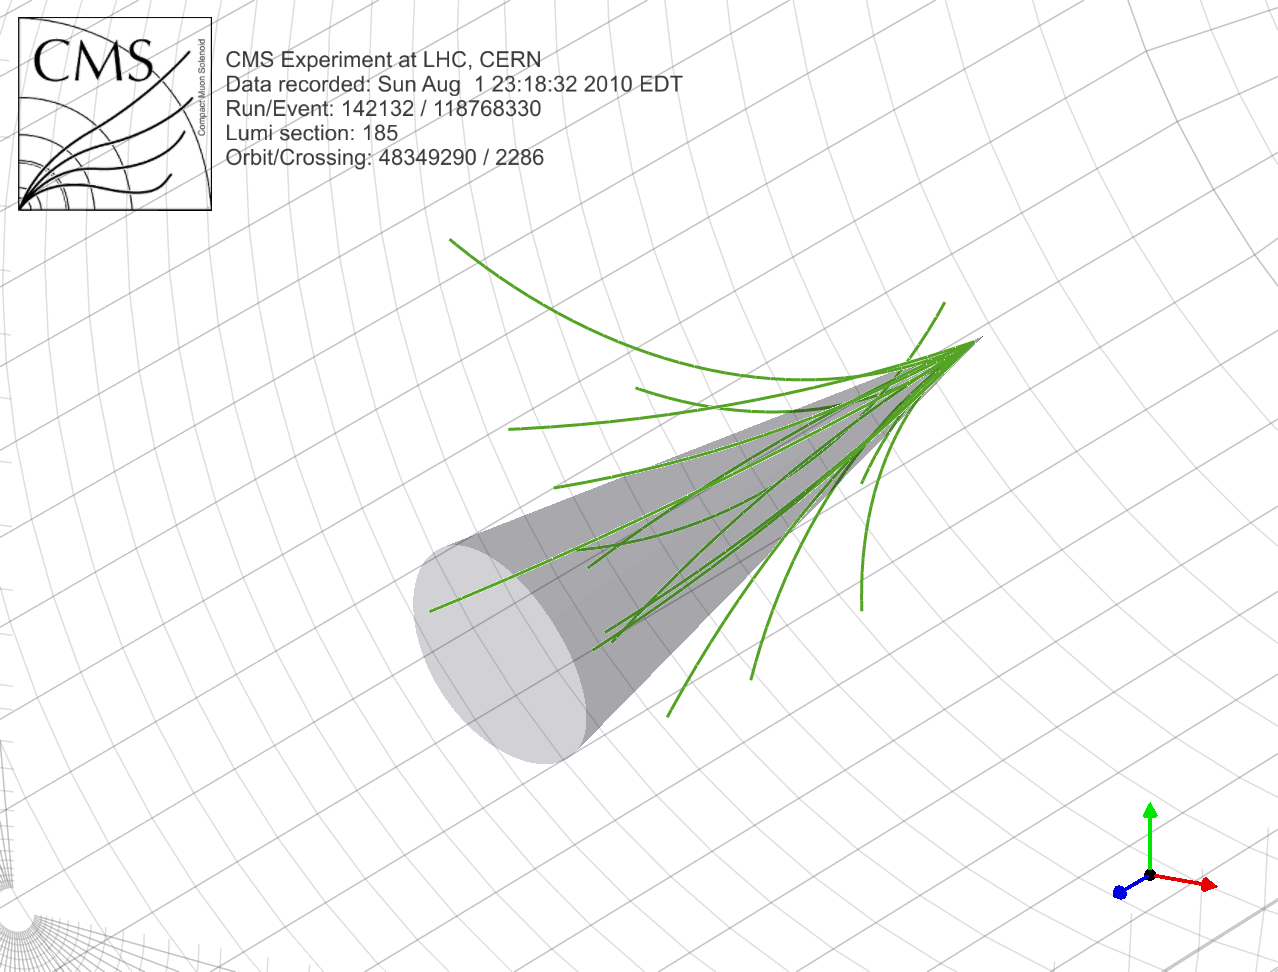
\includegraphics[width=\textwidth]{\figpath/Chapter4/JetConeWithTracks.png}
        \caption{}
        \label{fig:jc_track}
    \end{subfigure}
    \begin{subfigure}[t]{0.32\textwidth}
        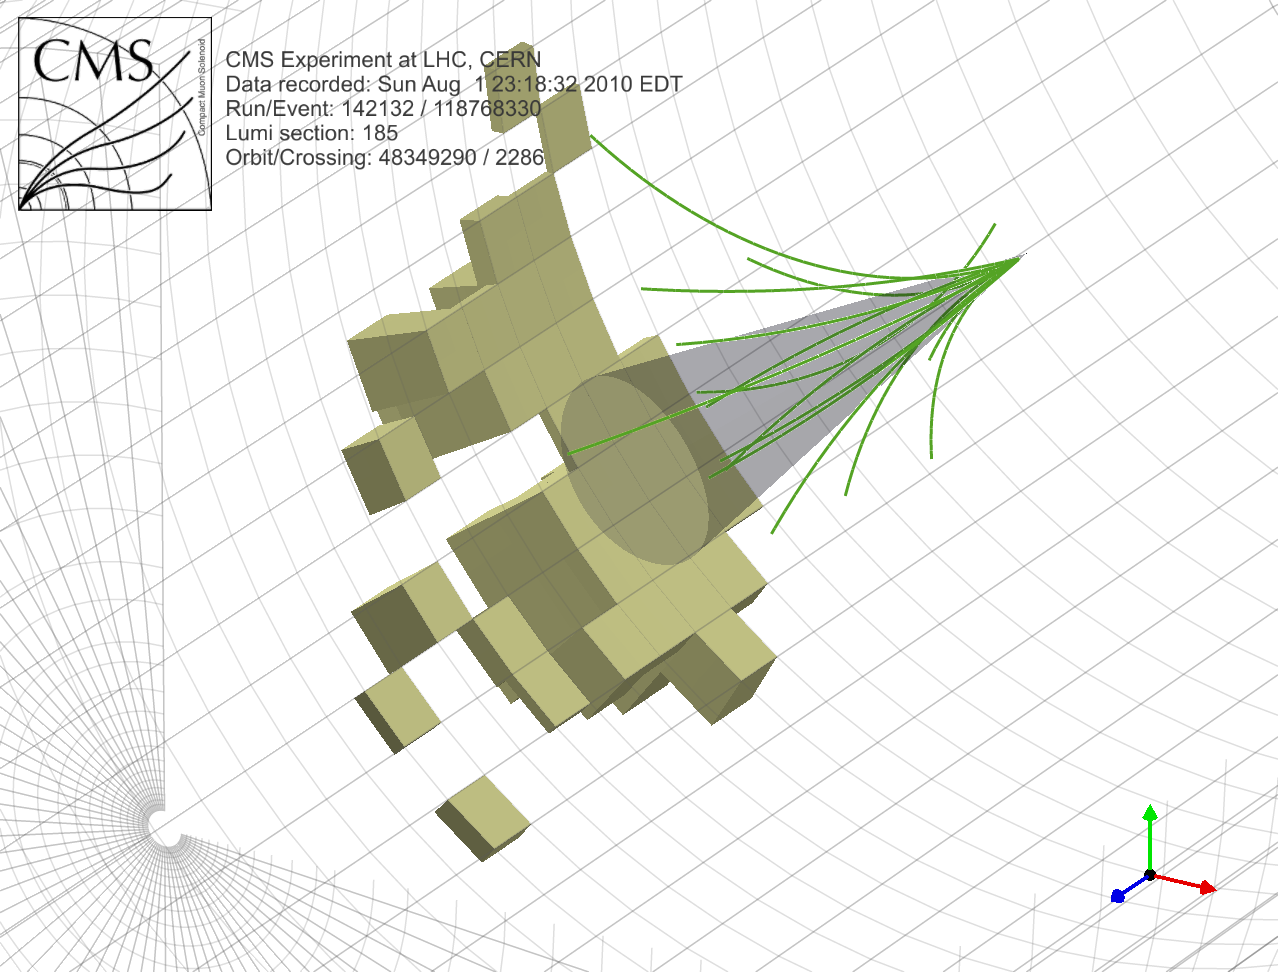
\includegraphics[width=\textwidth]{\figpath/Chapter4/JetConeWithTracksAndECAL.png}
        \caption{}
        \label{fig:jc_track_ecal}
    \end{subfigure}
    \begin{subfigure}[t]{0.32\textwidth}
        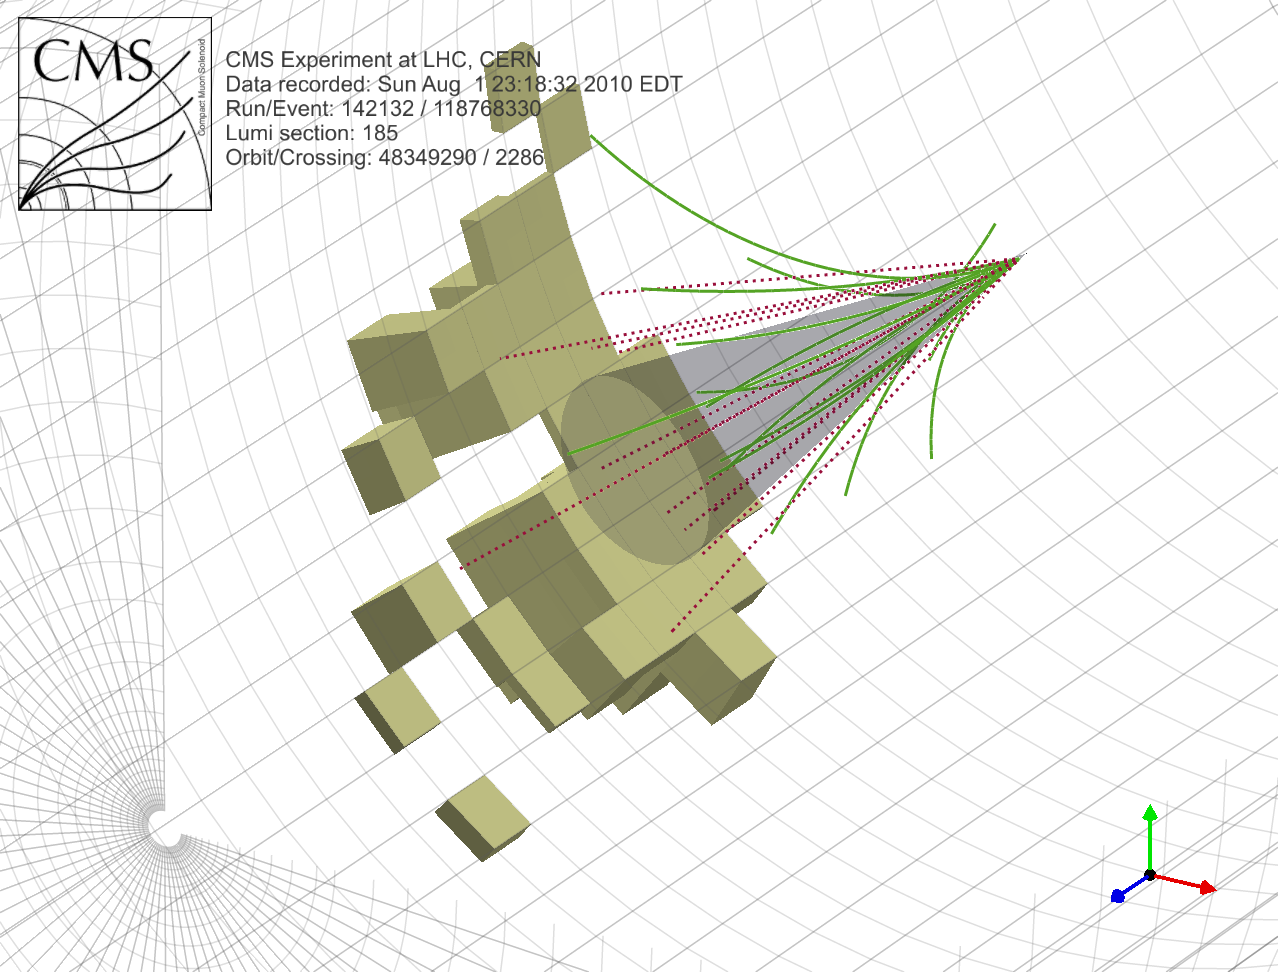
\includegraphics[width=\textwidth]{\figpath/Chapter4/JetConeWithTracksAndPhotonsAndECAL.png}
        \caption{}
        \label{fig:jc_track_photon_ecal}
    \end{subfigure}

    \begin{subfigure}[t]{0.32\textwidth}
        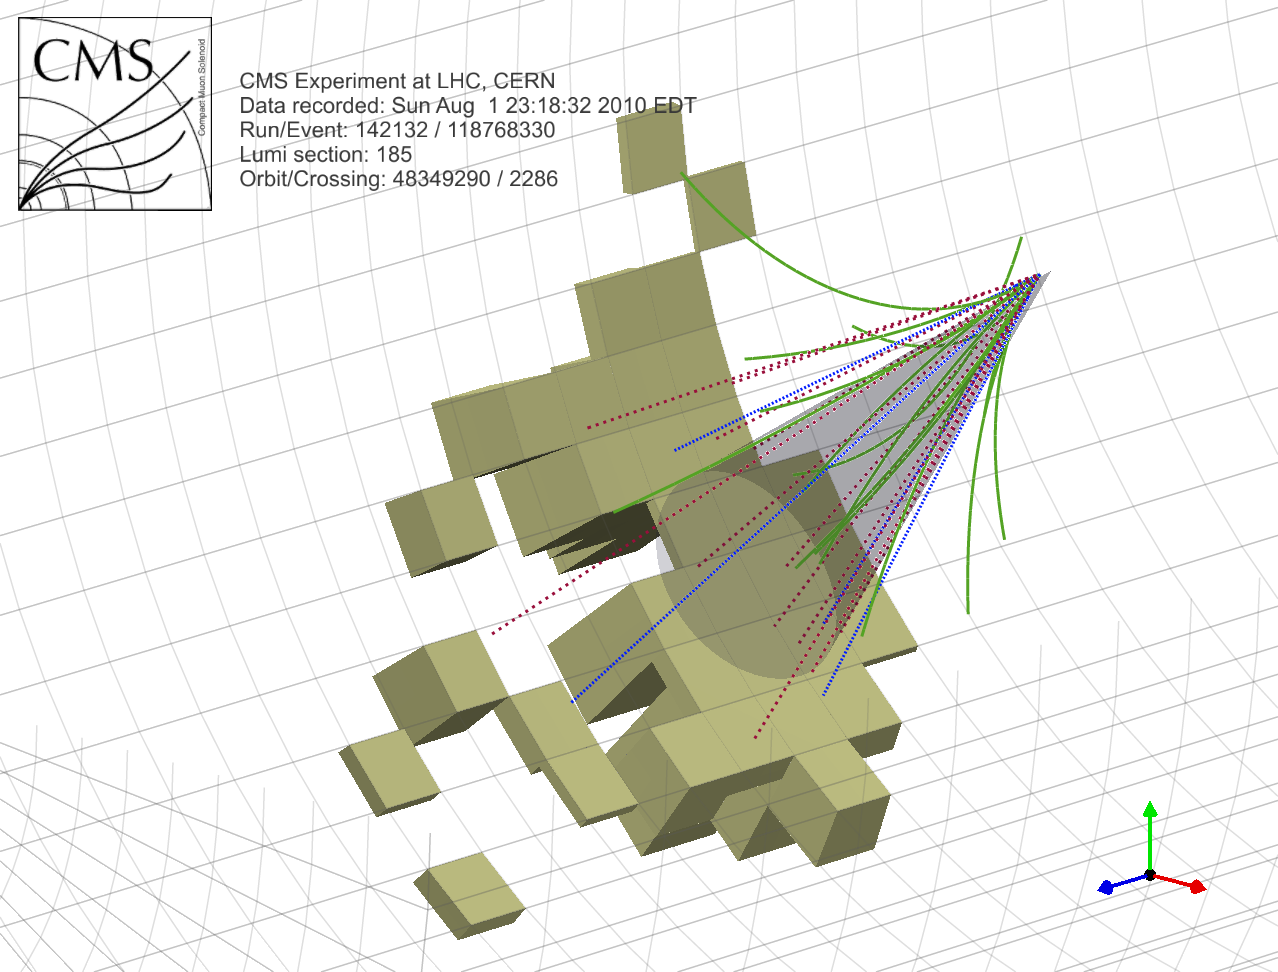
\includegraphics[width=\textwidth]{\figpath/Chapter4/JetConeWithTracksAndPhotonsAndNeutralHAndECAL.png}
        \caption{}
        \label{fig:jc_track_photon_neutralH_ecal}
    \end{subfigure}
    \begin{subfigure}[t]{0.32\textwidth}
        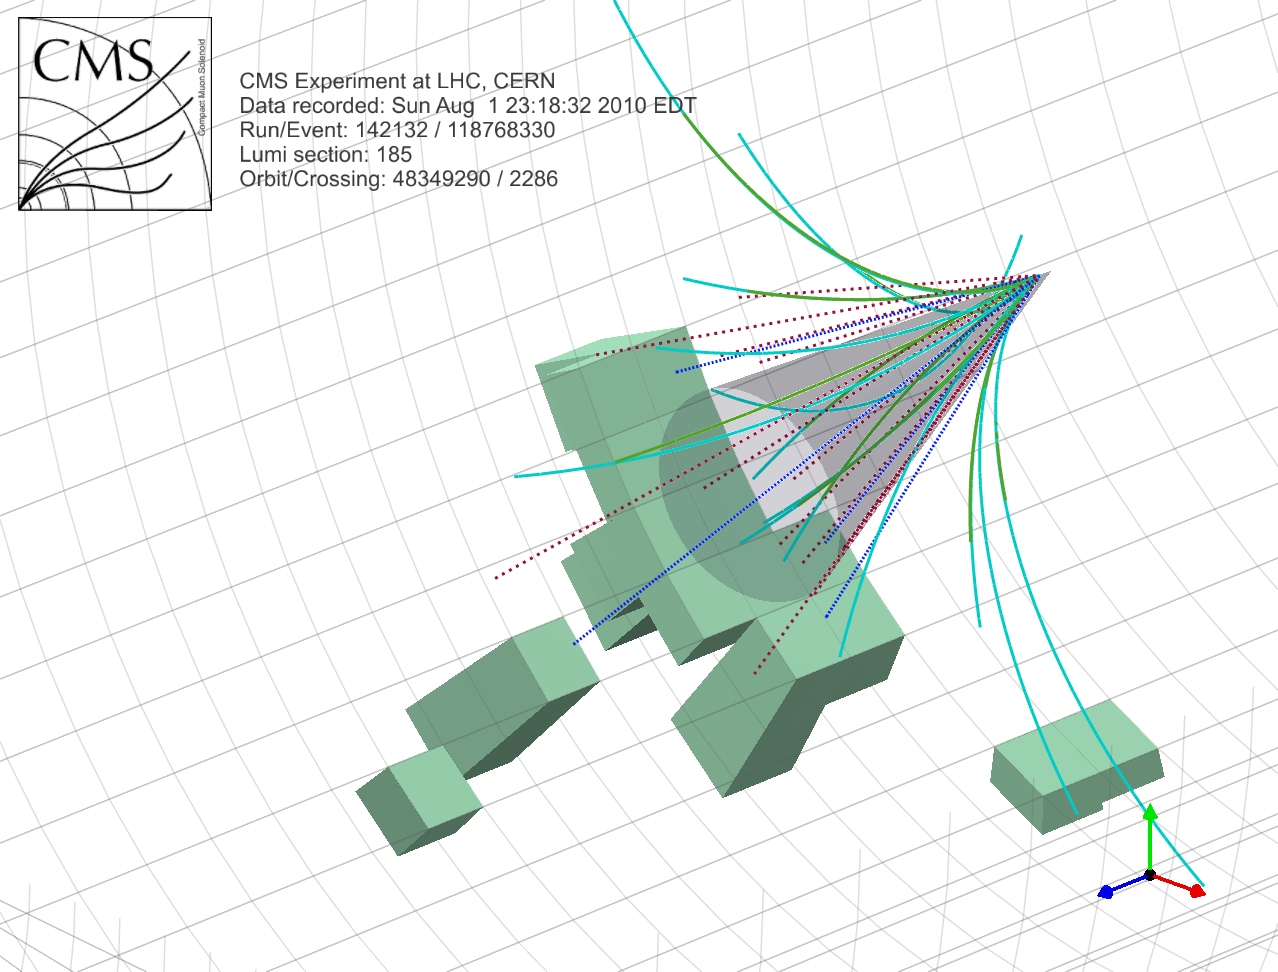
\includegraphics[width=\textwidth]{\figpath/Chapter4/JetConeWithTracksAndPhotonsAndNeutralHAndChargedHAndHCAL.png}
        \caption{}
        \label{fig:jc_track_photon_neutralH_chargedH_hcal}
    \end{subfigure}
    \begin{subfigure}[t]{0.32\textwidth}
        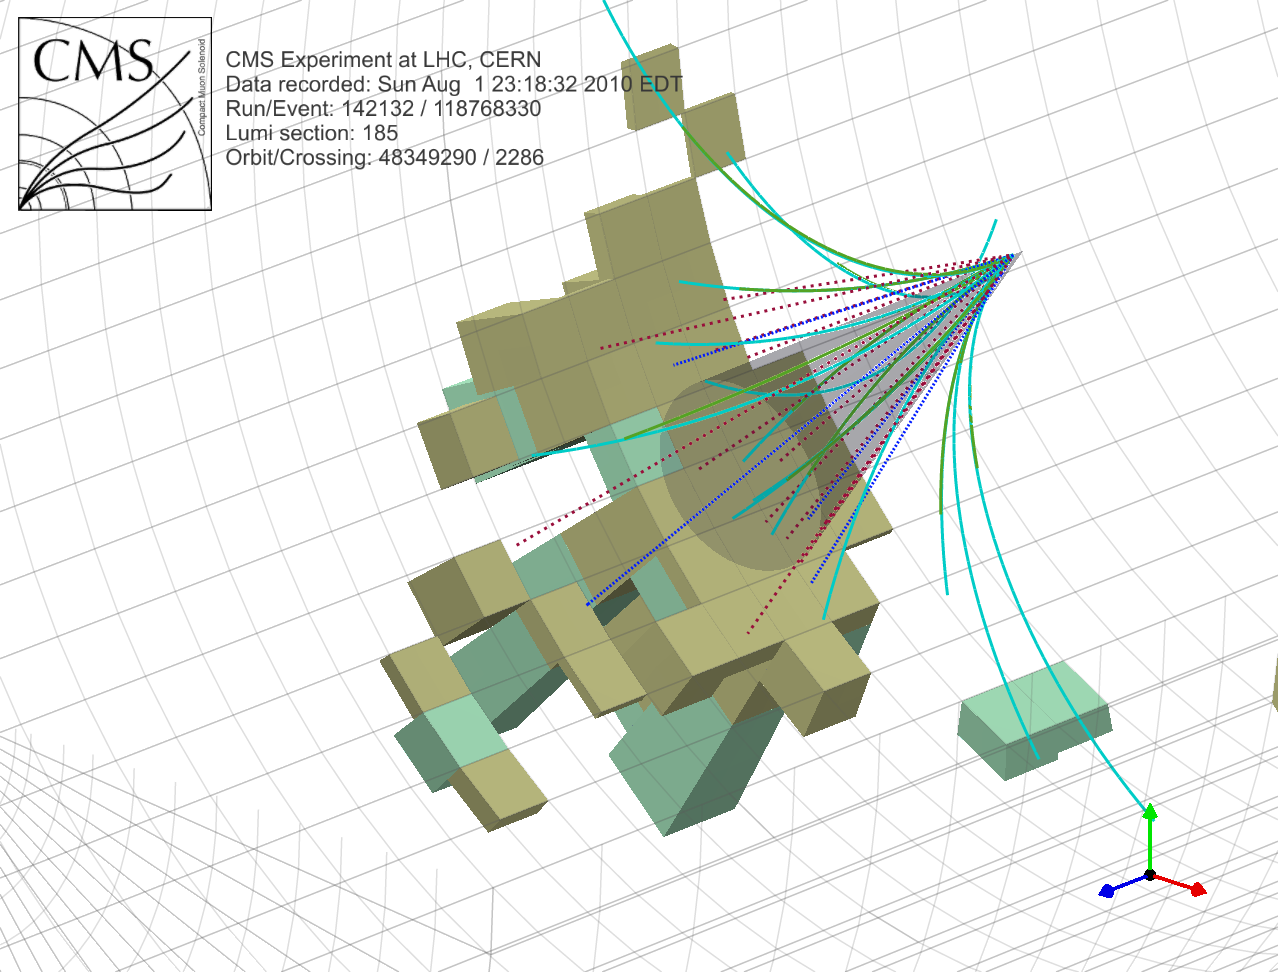
\includegraphics[width=\textwidth]{\figpath/Chapter4/JetConeAll.png}
        \caption{}
        \label{fig:jc_all}
    \end{subfigure}

    \begin{subfigure}[t]{0.32\textwidth}
        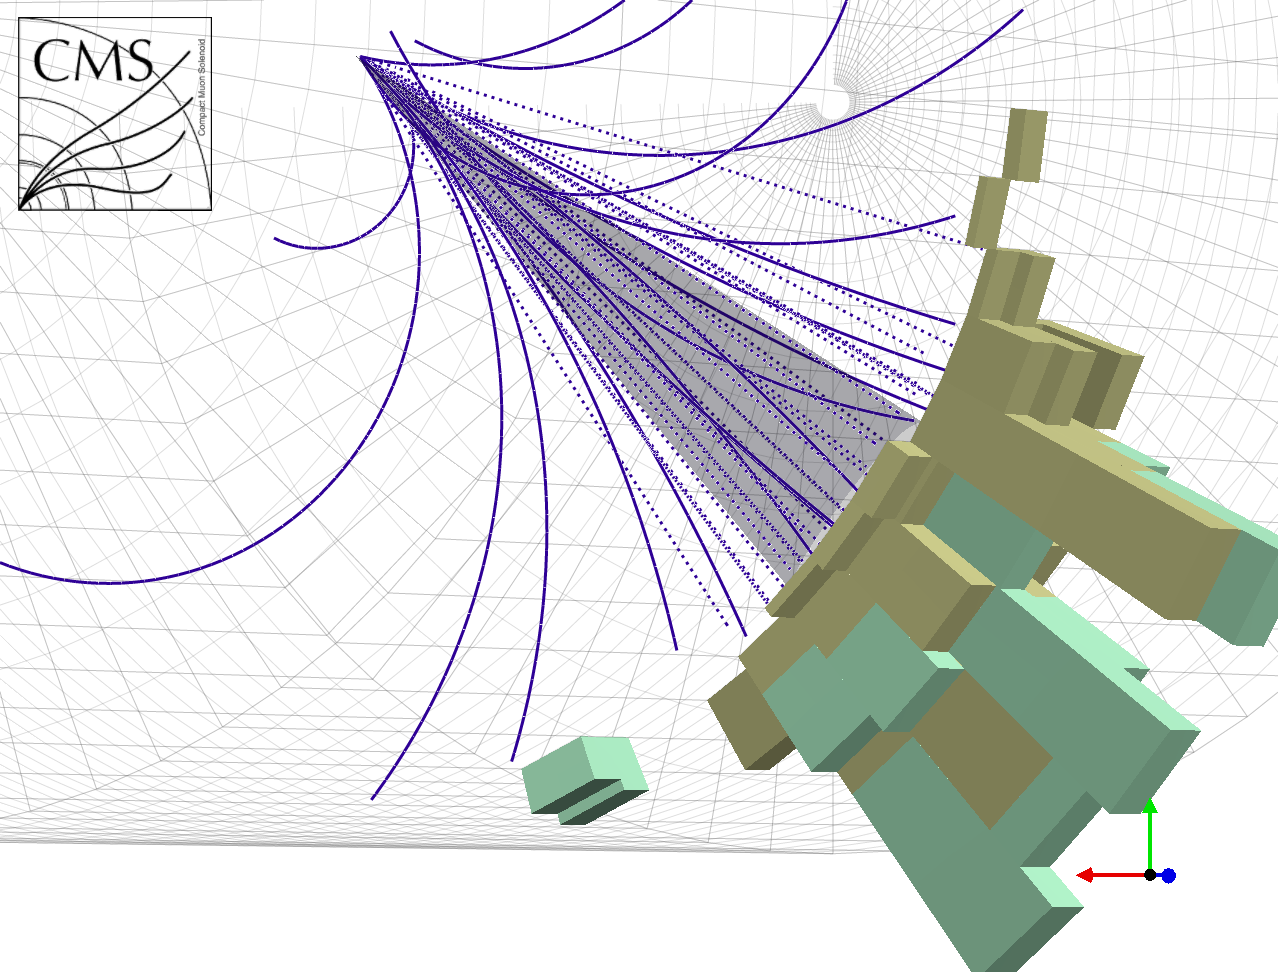
\includegraphics[width=\textwidth]{\figpath/Chapter4/JetConeAndPFJetCALVIEW1.png}
        \caption{}
        \label{fig:jc_PFjet1}
    \end{subfigure}
    \begin{subfigure}[t]{0.32\textwidth}
        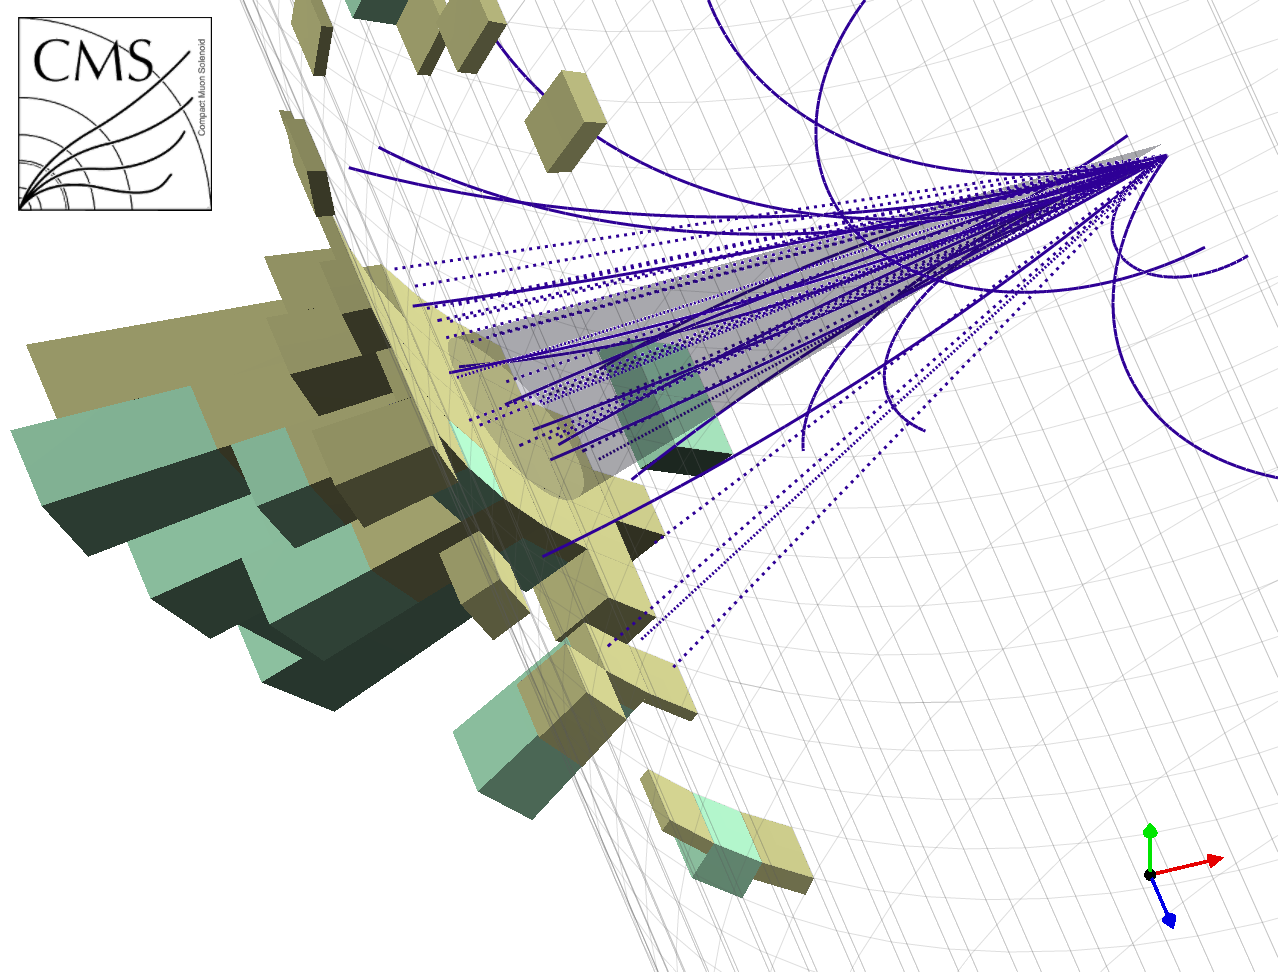
\includegraphics[width=\textwidth]{\figpath/Chapter4/JetConeAndPFJetCALVIEW3.png}
        \caption{}
        \label{fig:jc_PFJet3}
    \end{subfigure}
    \begin{subfigure}[t]{0.32\textwidth}
        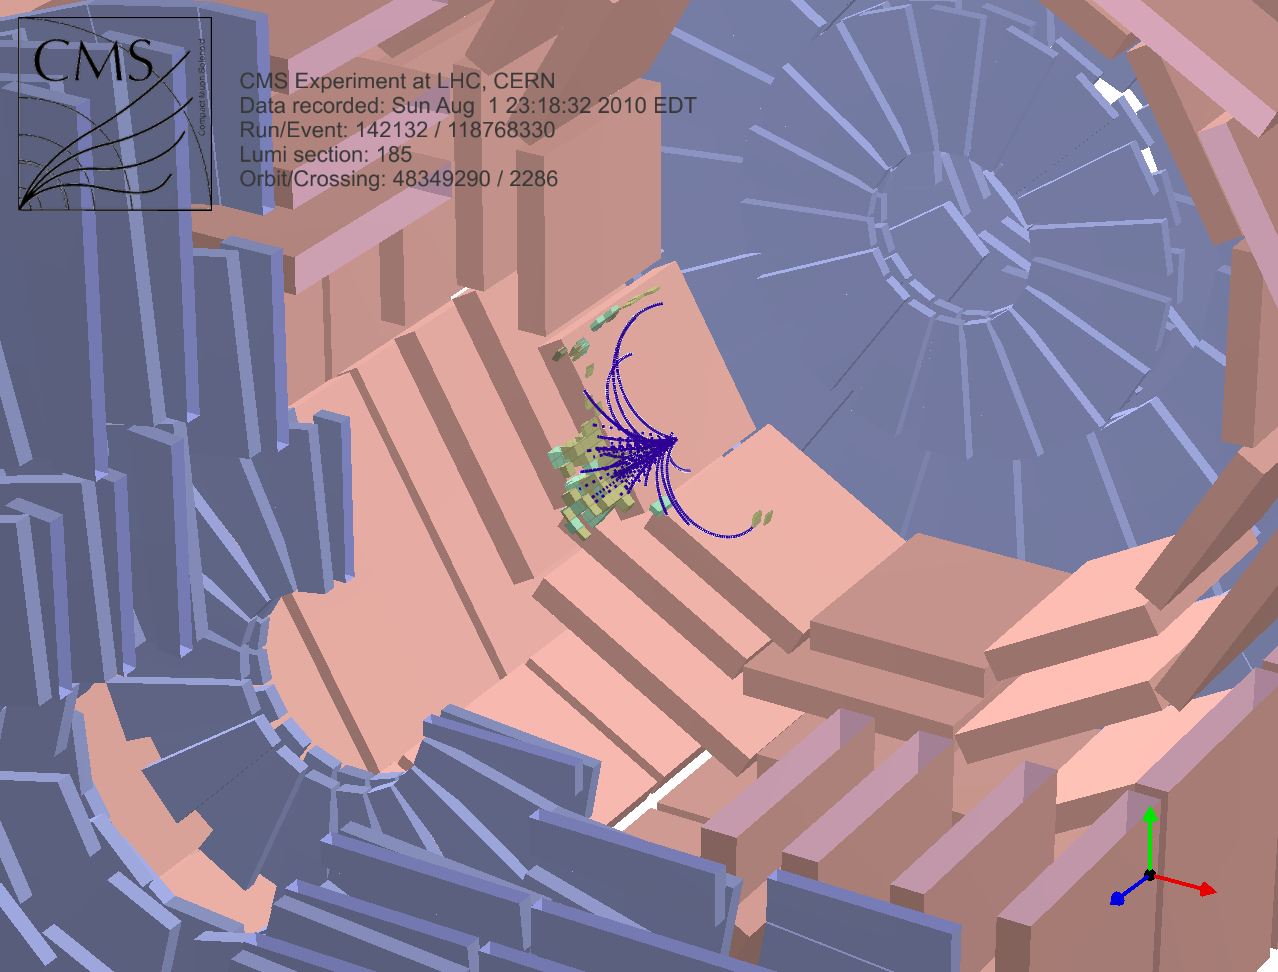
\includegraphics[width=\textwidth]{\figpath/Chapter4/JetWithFullDetector.png}
        \caption{}
        \label{fig:jet_fullDetector}
    \end{subfigure}
    \caption{Different views of the same 115\gev PF jet are shown with varying amounts of information displayed. The panels are ordered sequentially from left to right and top to bottom where each subsequent panel includes additional information. The image is of a jet with its (a) tracks, (b) ECAL deposits, (c) photon candidates, (d) neutral hadrons. Panel (e) shows the jet with its charged hadrons, but replacing the ECAL deposits for the HCAL deposits. Panels (f)-(h) show various views of the same jet with all of its constituents, while panel (i) shows the jet as it would appear in the CMS detector. The distance between the primary vertex and the interior of the red muon chambers is 7.5\unit{m} and the calorimeter deposits are scaled to about 10\unit{\gev/m}~\cite{Dorney2014}.}
    \label{fig:BuildingAPFJet}
\end{figure}

While the best way to cluster the cascade is still an open topic of discussion\footnote{Researchers are constantly asking themselves, "What is a jet?" The question is referring more to the idea of how to reconstruct a jet rather than the concept of a jet.}, this analysis clusters PF candidates using the anti-k\textsubscript{T} algorithm~\cite{Cacciari:2008gp} as defined in the \textsc{Fast}\textsc{Jet} package~\cite{Cacciari:2011ma}\footnote{In addition to providing fast, sequential clustering algorithms, the \textsc{Fast}\textsc{Jet} package is able to calculate the jet area, which is a non-trivial quantity~\cite{Cacciari2008}.}.
The anti-k\textsubscript{T} is a sequential recombination clustering algorithm which is both infrared and collinear safe.
Infrared safety means that the jet clustering algorithm is insensitive to the emission of soft, wide angle particles.
In other words, the jet is invariant under $\vec{p}_{i}\rightarrow\vec{p}_{j}+\vec{p}_{k}$, where the particle with momentum $\vec{p}_{i}$ split into two particles, each carrying momentum $\vec{p}_{j}$ and $\vec{p}_{k}$ respectively.
As an example, two jets should not be merged together just because one of them produced a 1\gev particle between them.
Collinear safety means that if there is a splitting which results in two parallel high-\pt particles, a single jet is produced and the jet properties will not be different from a jet where this splitting did not occur.
When an algorithm obeys these two properties, they are referred to as being IRC safe.
Simply put, the anti-k\textsubscript{T} algorithm results in jets which have physical properties (i.e. \pt, mass, etc.) that are representative of the partons in the event.

The use of PF candidate, with their built in tracking information, provides a huge benefit to the reconstruction and clustering of jets in CMS. About 65\% of the energy within a jet is carried by the charged particles and thus a lot of information about a jet comes from the tracker.\footnote{25\% of the energy is carried by photons and the remaining 10\% is carried by neutral hadrons.} An alternative to clustering PF candidates is to cluster the energy deposits in the calorimeter towers, but that provides both less spacial information as well as a lower response, where jet response is defined as $\left<\left(\ptsup{reco}-\ptsup{gen}\right)/\ptsup{gen}\right>$ and $\ptsup{reco}$ ($\ptsup{gen}$) is the reconstructed (generated) \pt. Fig.~\ref{fig:PFVsCaloJetResponse} shows a comparison of the PF based jet response (PF jets) versus calorimeter based jet responses (calo jets). The use of tracking information also improves the jet resolution, where typical values for a PF jet are 15\% at 10\GeV, 8\% at 100\GeV, and 4\% at 1\TeV. This is compared to about 40\%, 12\%, and 5\% when using calo jets~\cite{CMS-PAS-PFT-09-001}. A comparison of the resolution curves can be see in fig.~\ref{fig:PFVsCaloJetResolution}.

\begin{figure}[!hbt]
    \centering
    \begin{subfigure}[t]{0.48\textwidth}
        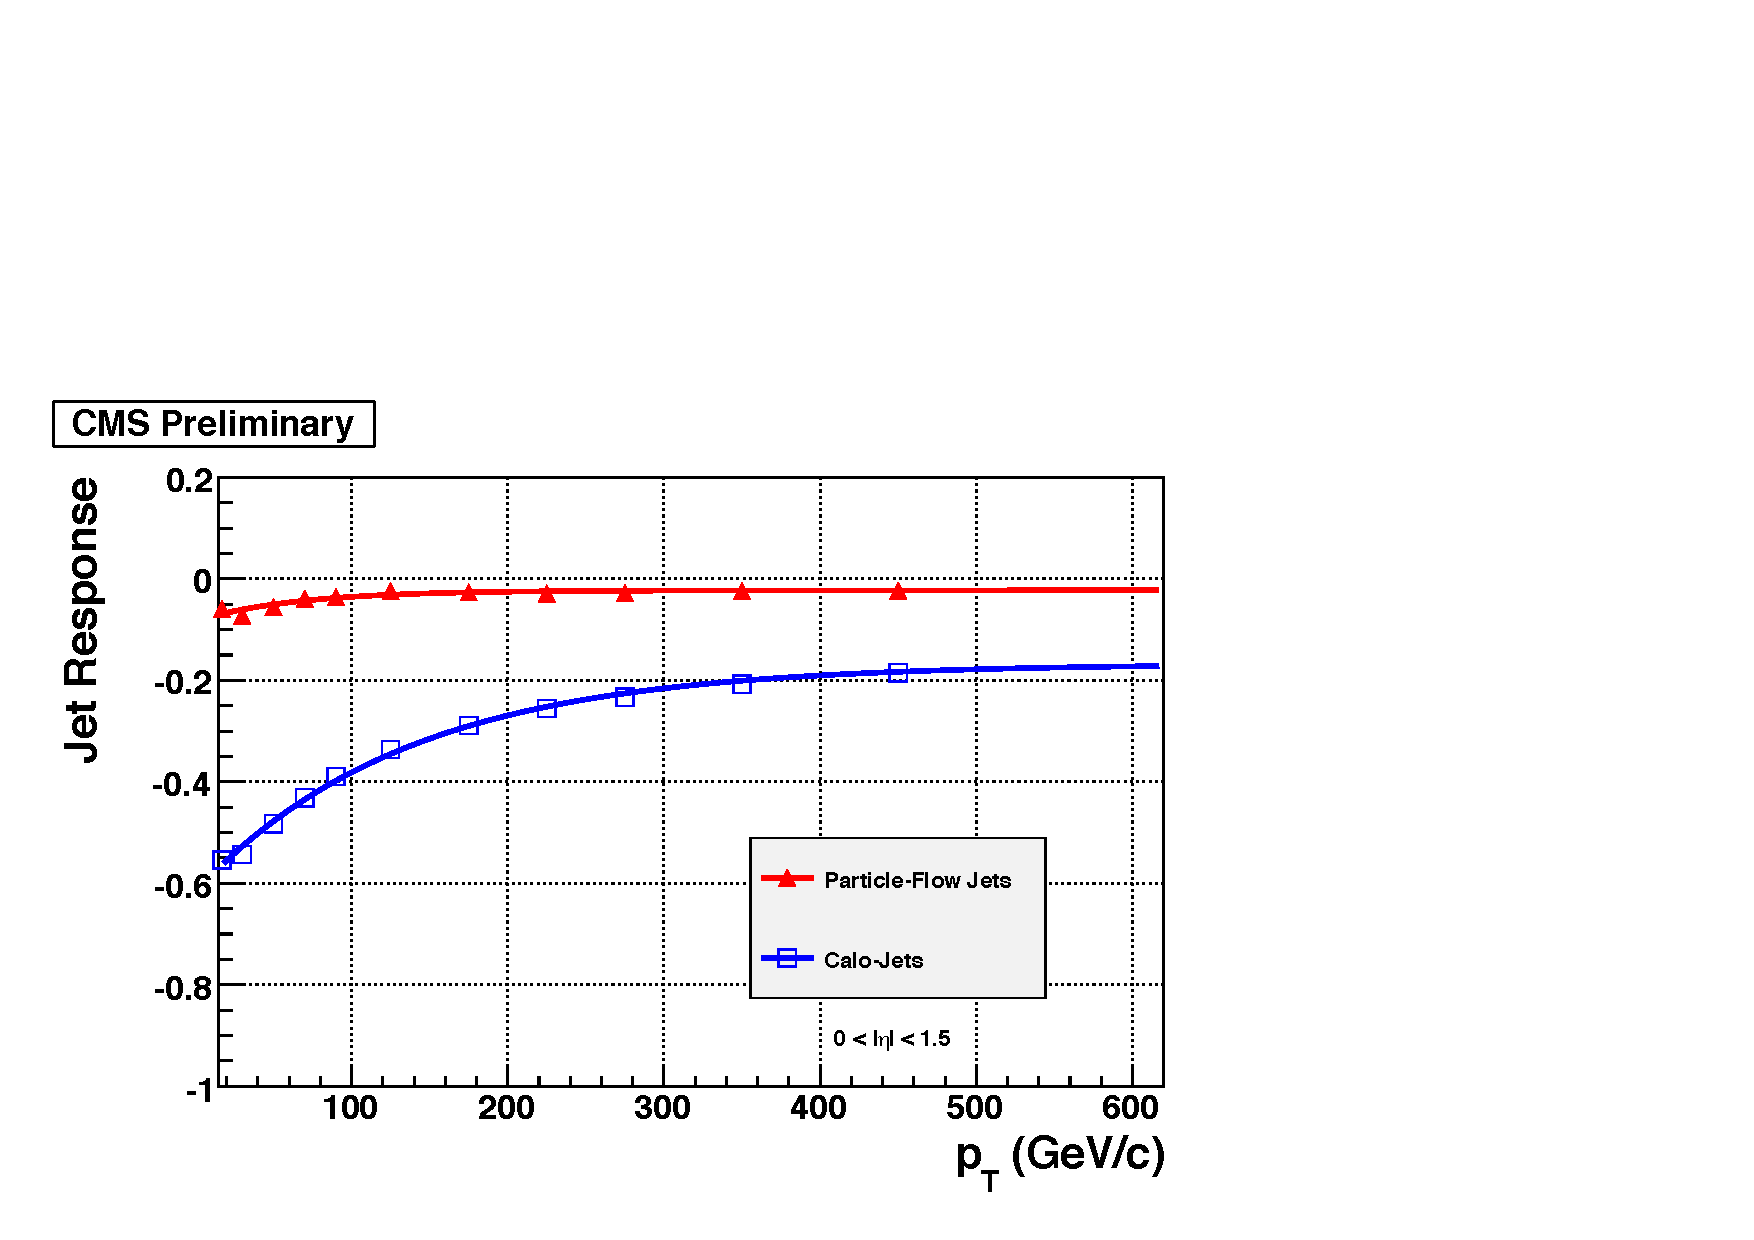
\includegraphics[width=\textwidth]{\figpath/Chapter4/Figure_008-b.pdf}
        \caption{}
        \label{fig:PFVsCaloJetResponse}
    \end{subfigure}
    \begin{subfigure}[t]{0.48\textwidth}
        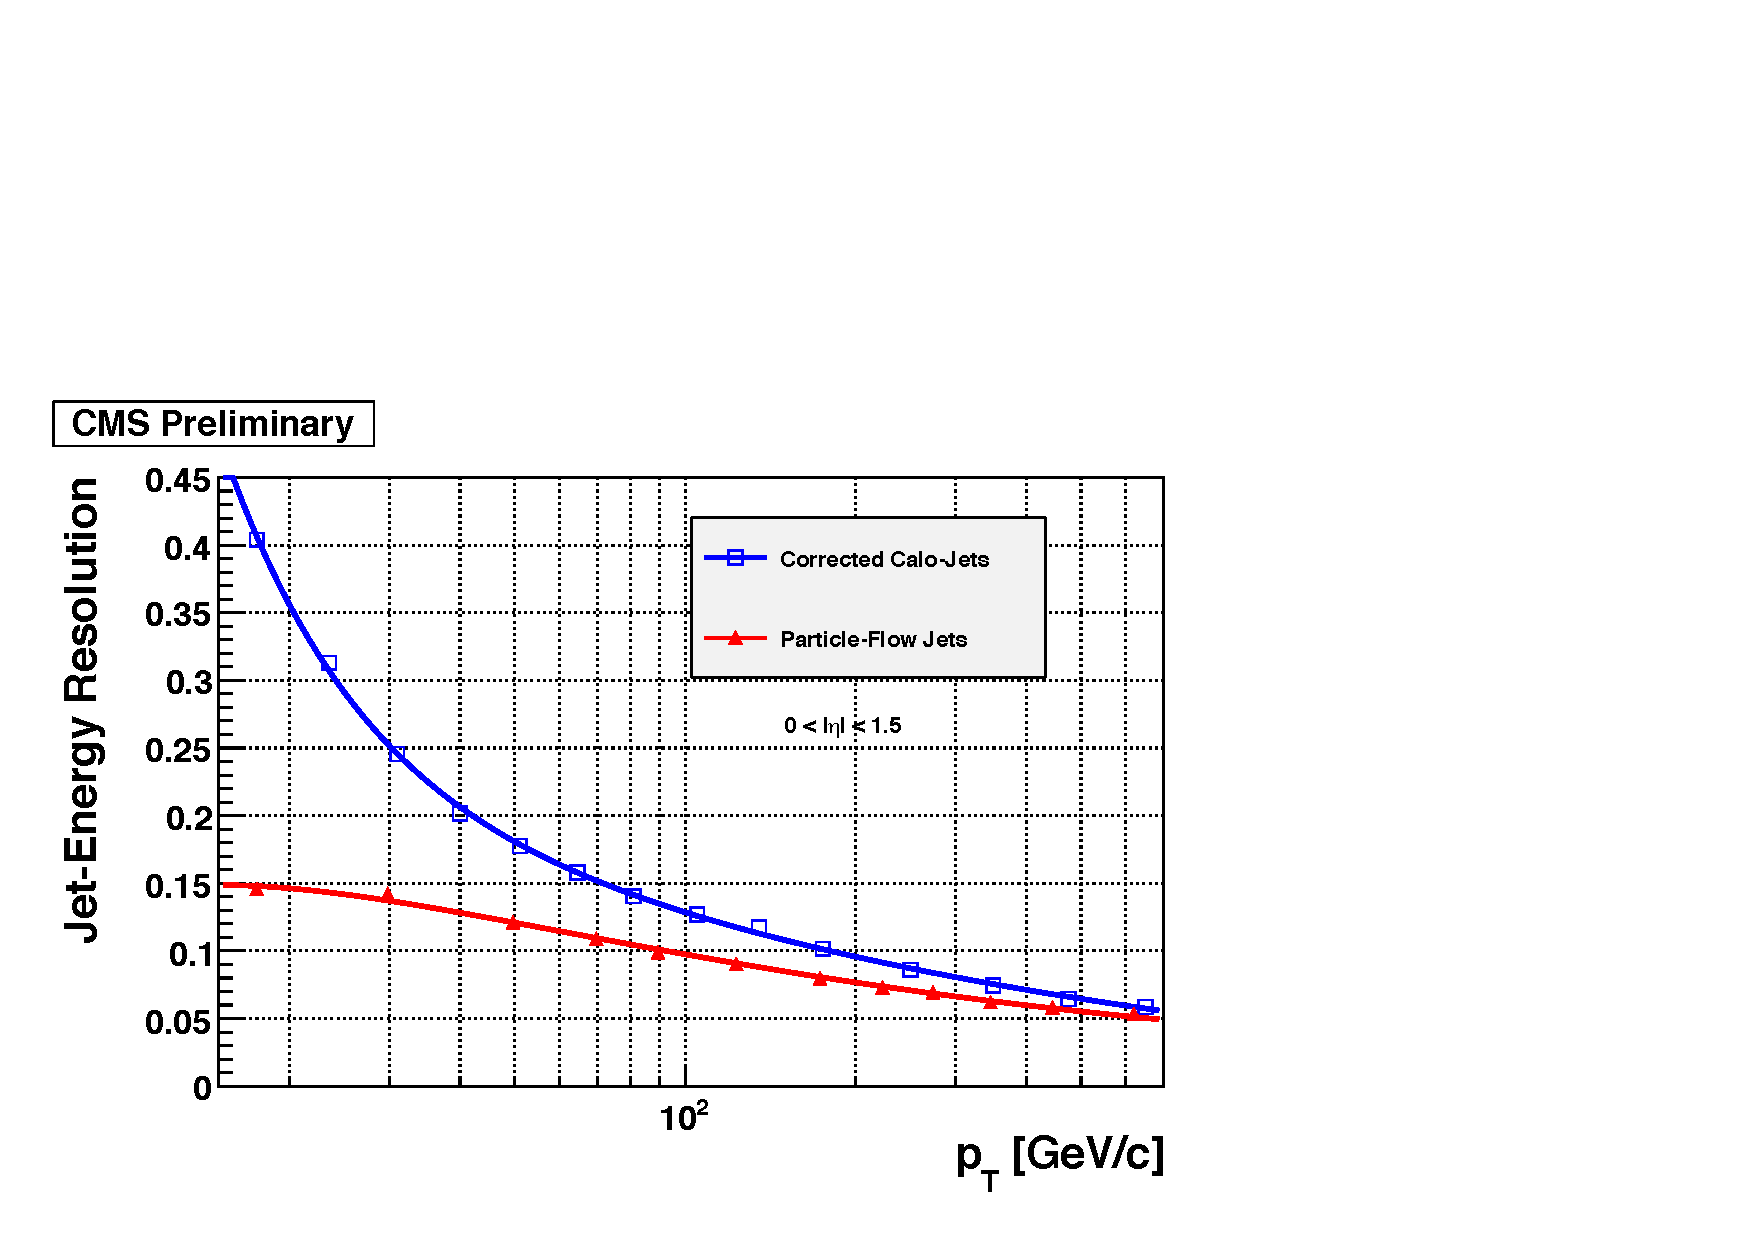
\includegraphics[width=\textwidth]{\figpath/Chapter4/Figure_010-a.pdf}
        \caption{}
        \label{fig:PFVsCaloJetResolution}
    \end{subfigure}
    \caption{Jet response (left) and resolution (right) as a function of \pt for jets made by clustering PF candidates and those clustering calorimeter towers. These figures were made using a MC sample with a center-of-mass energy of 10\tev, requiring the jets' \pt to be less than 750\gev, and that the jets are within \absetalt{1.5}~\cite{CMS-PAS-PFT-09-001}.}
\end{figure}

Before clustering the PF candidates, a pileup mitigation algorithm called charged hadron subtraction (CHS) is performed. As discussed in section~\ref{sec:tracks_and_vertices}, CMS can associate a track to a specific vertex. If these tracks are unambiguously associated to a pileup vertex, they are removed from the collection of PF candidates used to cluster jets and calculate the \VETslash. As shown in fig.~\ref{fig:PFJet_PileupComposition}, the CHS algorithm is able to remove about 50\% of the pileup energy produced during the same bunch crossing as the primary vertex. Any remaining energy from charged hadrons is coming from tracks that are not associated with a high quality vertex or which simply have too large a $\chi^{2}/N_{dof}$. Some of this is explained by the vertex reconstruction and identification inefficiency of about 30\%~\cite{Khachatryan:2198719}.

\begin{figure}[!hbt]
    \centering
    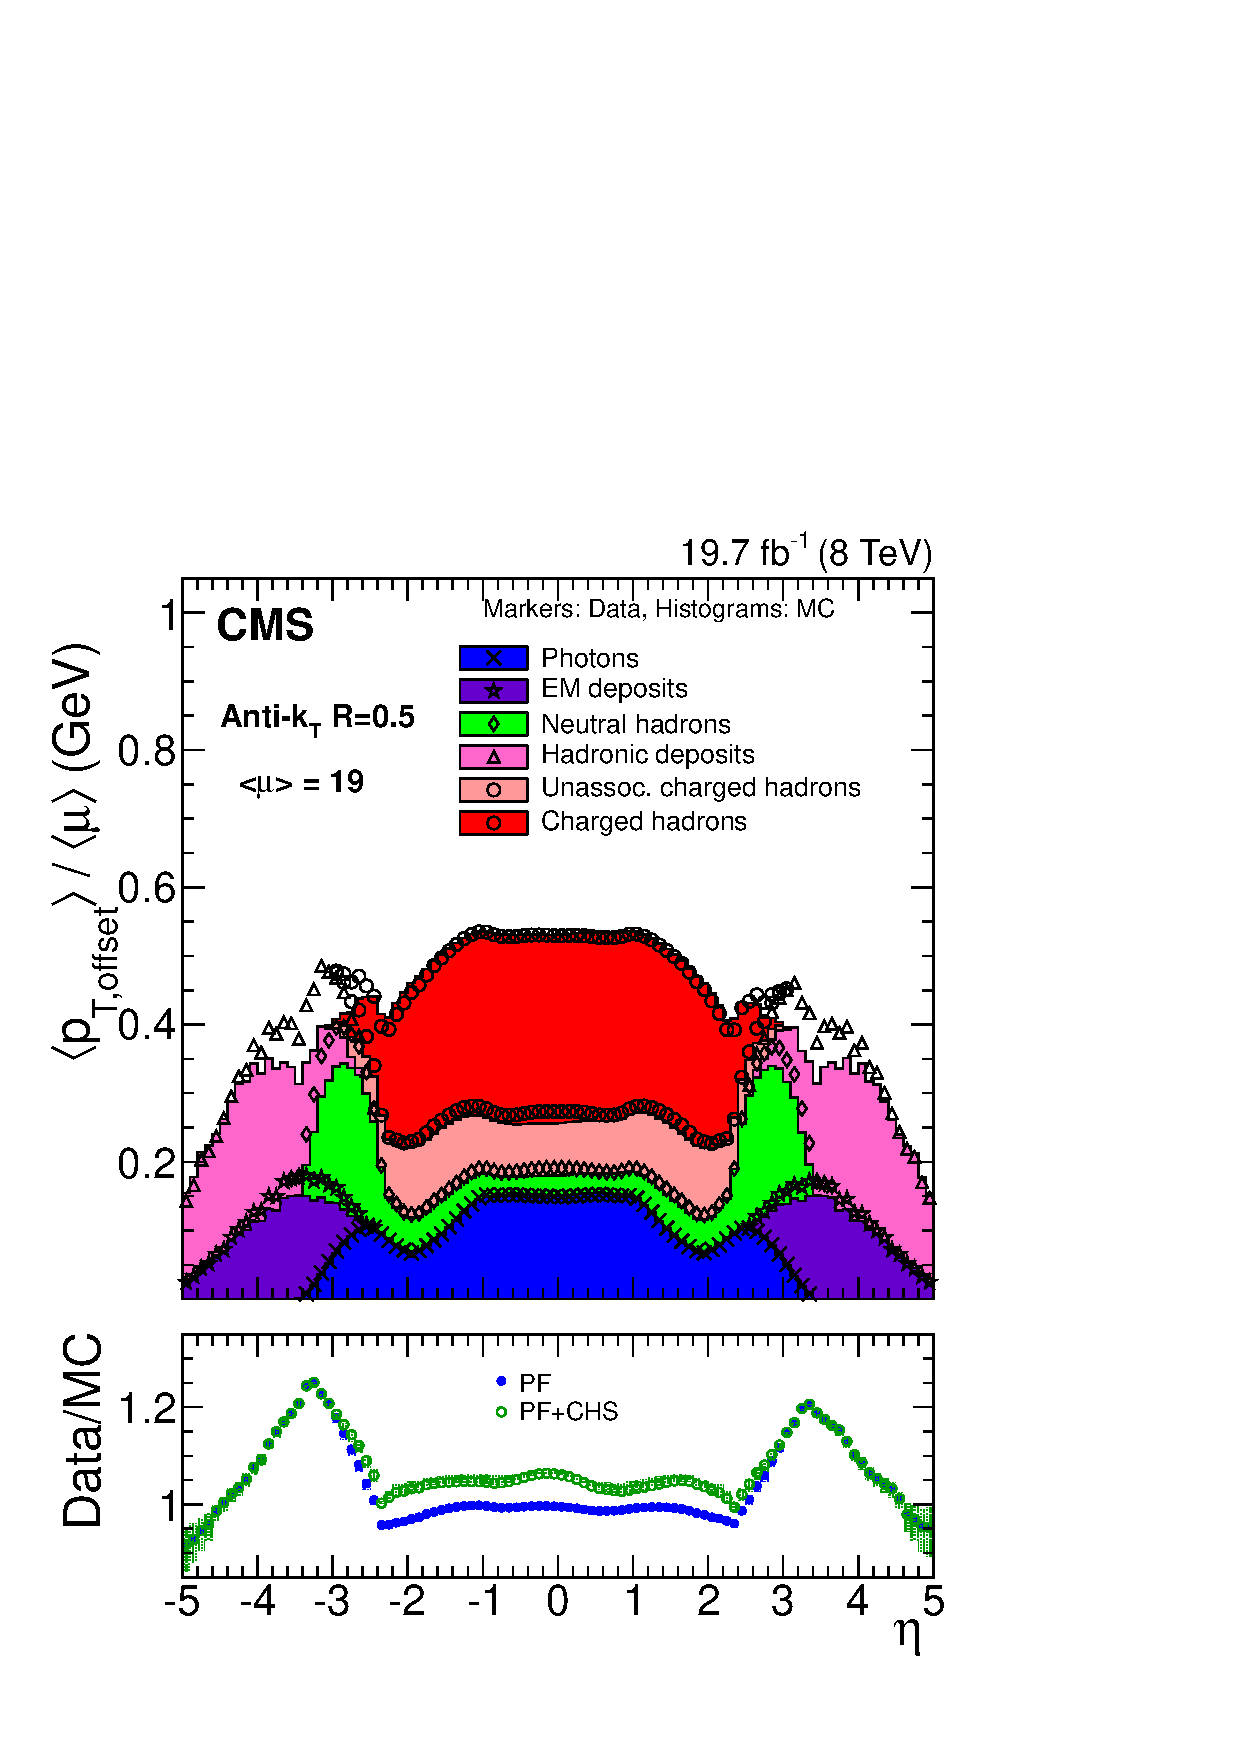
\includegraphics[width=0.95\textwidth]{\figpath/Chapter4/OffsetPerPU_Stacked_twopad_NPU-6_NPU-35.pdf}
    \caption{Pileup energy within a jet per additional proton-proton interaction ($\mu$) separated by type PF type. The fraction labeled ``charged hadrons'' will be removed by the CHS algorithm. The ratio of the data to the simulation is shown in the lower panel~\cite{Khachatryan:2198719}.}
    \label{fig:PFJet_PileupComposition}
\end{figure}

Like most other clustering algorithms (i.e. k\textsubscript{T}, Cambridge/Aachen, SisCone, etc.), anti-k\textsubscript{T} is iterative, wherein at each iteration two distance parameters are calculated.
$d_{ij}$ and $d_{iB}$, as defined in equation~\ref{eq:antikt_distance_parameter}, are the distance between two entities (PF candidates or existing cluster) and the distance from any one entity and the beam, respectively.
$y$ is the rapidity and R is a radius parameter, which is 0.5 in this analysis.
The anti-\textsubscript{T} algorithm is achieved when $p=-1$, whereas if $p=1$ ($p=0$) the k\textsubscript{T} (Cambridge/Aachen) algorithm is used instead.
If $d_{ij}<d_{iB}$, then entity $i$ and $j$ are combined vectorially.
However, if $d_{ij}>d_{iB}$, then entity $i$ is classified as a jet and is removed from further clustering.
This process continues until all PF candidates have been clustered~\cite{Cacciari:2008gp} and the momentum of the jet is the vectorial sum of all of the PF candidate momenta.
The result of this process can be seen in fig.~\ref{fig:anti-kT_jets}.

\begin{subequations}
    \label{eq:antikt_distance_parameter}
    \begin{align}
\label{eq:antikt_distance_parameter_1}d_{iB}={}&{p_{T}}_{i}^{2p}\\
\label{eq:antikt_distance_parameter_2}d_{ij}={}&min\left({p_{T}}_{i}^{2p},{p_{T}}_{j}^{2p}\right)\frac{\left(y_{i}-y_{j}\right)^{2}+\left(\varphi_{i}-\varphi_{j}\right)^{2}}{R^{2}}
    \end{align}
\end{subequations}

\begin{figure}[!hbt]
    \centering
    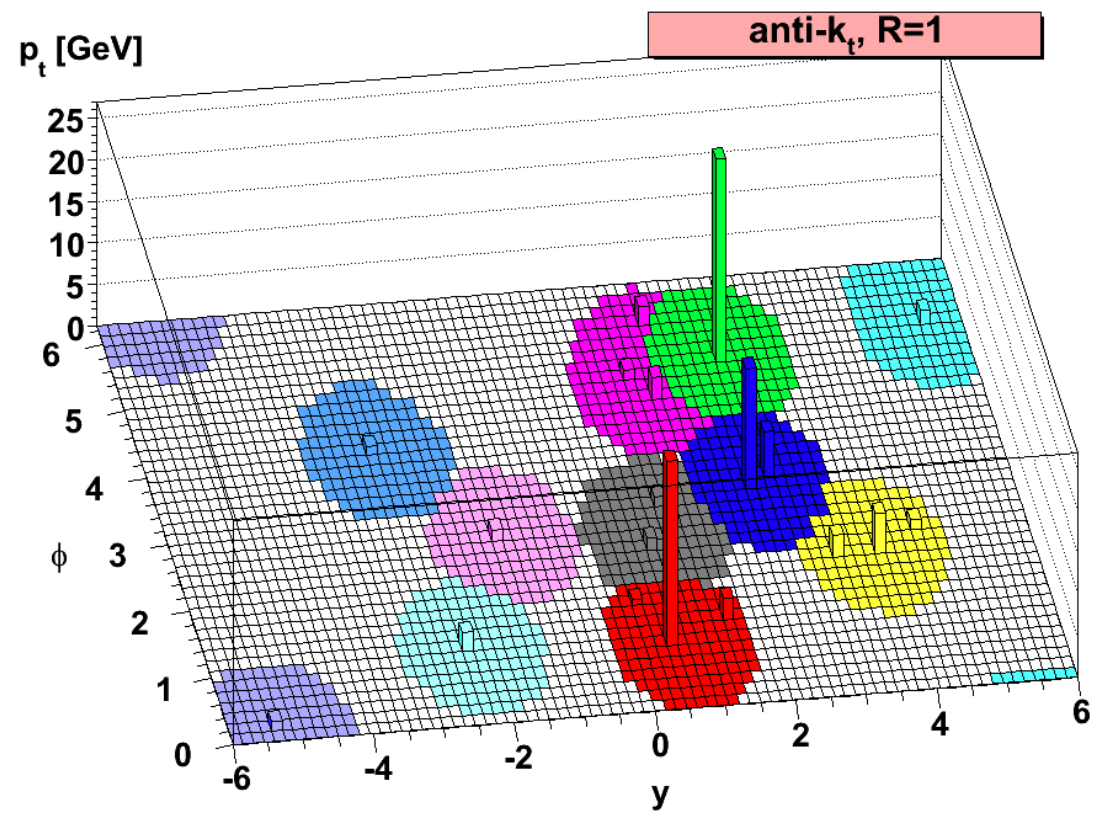
\includegraphics[width=0.95\textwidth]{\figpath/Chapter4/Anti-kT_Jets.png}
    \caption{Jets clustered from generator level partons using the anti-k\textsubscript{T} algorithm. This produces roughly circular jets with stable areas that are insensitive to additional soft particles~\cite{Cacciari:2008gp}.}
    \label{fig:anti-kT_jets}
\end{figure}

After CHS and clustering the momentum and energy of the jets still might not be the same as those from the initial parton, whether because of pileup or detector effects.
To correct for this, CMS uses a factorized approach, wherein each level of correction targets a specific effect and each correction is applied in order.
The goal is to make sure each jet has a relative response ($RelRsp=\frac{\ptsup{reco}}{\ptsup{gen}}$) of 1.
This type of scaling is commonly referred to as a jet energy correction (JEC)\footnote{The terms \pt and energy will be used interchangeably only when discussing the jet energy corrections. This is because the corrections will affect both the energy and \pt terms within the jet 4-momentum.}.
The first level of correction, commonly referred to as the L1FastJet corrections, starts by removing any remaining pileup\footnote{CHS was able to remove pileup energy coming from charged hadrons, but not energy added to the jet from, for example, neutral hadrons or photons as seen in figure~\ref{fig:PFJet_PileupComposition}.} or electronic noise energy that may have made it into the jet reconstruction.
This multiplicative correction will only remove energy from within the jet and will take the form in equation~\ref{eq:JEC_L1FastJet}, where $\rho$ is the median energy density of the event, $A$ is the jet area, and $f$ is an estimate of the offset inside the jet per unit of jet area~\cite{JINST2011,Cacciari2007}.
\begin{equation}
\label{eq:JEC_L1FastJet}
\ptsup{L1Corrected}=\ptsup{uncorrected}\cdot\left(1-A\frac{f\left(\eta,\rho,A\right)}{\ptsup{uncorrected}}\right)
\end{equation}
The L2Relative correction seeks to correct for the non-linearity in the jet response as a function of $\eta$ while the L3Absolute correction does the same thing as a function of \pt.
These are again multiplicative corrections that can either increase or decrease the energy of the jet.
All three corrections are applied to both data and simulation.
An additional level of correction, termed L2L3Residual, is applied only to data to correct for the difference in scale between the data and simulation.
Finally an $\eta$ dependent smearing factor is applied to the jets coming from the MC samples in order to make the jet energy resolution in MC match the jet energy resolution in data~\cite{JetEnergyResolutionTwiki}.
For a more in-depth discussion of pileup mitigation techniques and jet energy corrections see appendix~\ref{appendix:JERC}.

A set of quality cuts, collectively called PF jet identification, are applied to the resulting collection of jets to ensure that only real, hard scatter PF jets are used during the analysis~\cite{CMS-AN-2010-003}. Several working points are defined at varying levels of efficiency and purity, but this analysis makes use of the loose criteria shown in table~\ref{tab:PFJetID}~\cite{PFJetID}. The variables used in these cuts include the fraction of neutral hadrons in the jet $f_{NH}$, the fraction of neutral EM particles $f_{\gamma}$, the fraction of charged hadrons $f_{CH}$, the fraction of charged EM particles $f_{EM}$, the number of constituents $n_{constituents}$, and the multiplicity of charged particles $n_{charged}$. All cuts on the jet energy fractions are made on the raw jets, before any energy correction are applied. In addition to the PF jet quality cuts, this analysis requires that all jets be within \abseta{2.4}, the leading jet have $\pt>30\gev$, and all other jets have $\pt>25\gev$. Additionally, all jets are required to be at least ${\Delta}R(\textrm{jet},\textrm{lepton})>0.3$ away from any isolated, selected lepton.
\begin{table}[htbp]
    \caption{Cut based PF jet identification requirements for the loose working point.}
    \centering
    \begin{tabular}{ll}
        \hline
        \multirow{2}{*}{Cut Variable}               & Cut Value \\\cline{2-2}
                                                    & Loose \\
        \hline
        $f_{CH}>$                                  & 0.0        \\
        $f_{NH}<$                                  & 0.99 \\
        $f_{\gamma}<$                              & 0.99        \\
        $f_{EM}<$                                  & 0.99         \\
        $n_{charged}>$                              & 0          \\
        $n_{constituents}>$                         & 1           \\
        \hline
    \end{tabular}
    \label{tab:PFJetID}
\end{table}

\section{b-tagging}
\label{sec:btagging}

Bottom quarks are interesting because they are often associated with the decays of the top quark and the Higgs boson.
The experimental signature of a hadronizing bottom quark will be a \textit{b-jet}.
This flavor of jet is identifiable because of the unique decay kinematics of b hadrons, including their long lifetime (1.5\unit{ps}$\Rightarrow{c}\tau\approx450\mum$) and high \pt decay products~\cite{Olive:2016xmw,PhysRevD.17.171}.
Additionally, b hadrons have a relatively large mass ($\sim5\gev$), which means they have a higher track multiplicity than other quark jets, about 5 on average.
The displaced tracks will form a secondary vertex with a large impact parameter which can be measured by the tracking sub-detector.
CMS uses the Combined Secondary Vertex (CSV) algorithm to tag jets as either being initiated by a bottom quark or some other parton (u, d, s, c, and g)~\cite{Weiser:927399,BTV-12-001}.

In order to identify secondary vertices, the algorithm starts from a subset of well-reconstructed tracks.
These tracks must have a \pt greater than 1\gev, $\chi^{2}/N_{dof}<5$, a transverse (longitudinal) impact parameter less than 0.2\unit{cm} (17]\unit{cm}), and a $\Delta{R}$ to the jet axis less than 0.3.
Each track is also required to have at least 8 hits in the tracker, of which 2 must be from the pixel detector.
To reduce the effects of pileup the track's distance of closest approach to the jet axis (primary vertex) must be less than 700\mum (5\unit{cm}).
Once the tracks are selected, the secondary vertices are reconstructed using the AVF described in section~\ref{sec:tracks_and_vertices}.
At each iteration, if the track weight is greater than 0.5 the track is removed and the iterations continue until no more secondary vertices are found.
In order to increase the purity of the secondary vertices they are required to share no more than 65\% of their tracks with the primary vertex, to be more then $3\sigma$ away from the primary vertex in the $\eta-\varphi$ plane, and the $\Delta{R}$ between the vertex and the jet direction must be less than 0.5.
A secondary vertex candidate is also rejected is its radial distance to the primary vertex is greater than 2.5\unit{cm} and its invariant mass is close to that of the \PKz.
The jets are then assigned as being associated to a real secondary vertex, a \textit{pseudo-vertex}, or no vertex.
A \textit{pseudo-vertex} if created when the AVF fails to find a secondary vertex, but there are at least two tracks with $S_{ip}>2$, where $S_{ip}$ is the significance of the track's impact parameter defined as the value of the impact parameter divided by its uncertainty.

The following are used as inputs to the CSV tagger:
\begin{itemize}
    \item The significance of the flight distance in the transverse plane between the secondary and primary vertices.
    \item The invariant mass of the secondary vertex (the mass of all of the tracks associated with that vertex).
    \item The number of tracks associated to the secondary vertex.
    \item The ratio of the energy carried by the tracks associated to the secondary vertex and all tracks in the jet.
    \item The $\Delta\eta$ between the jet axis and the tracks associated to the secondary vertex.
    \item The transverse impact parameter significance of the tracks which raises the invariant mass above 1.5\gev, the charm threshold. The tracks are ordered by decreasing significance and combined one-by-one until the charm threshold is met.
    \item The number of tracks in the jet.
    \item The three-dimensional impact parameter significance of each track.
    \item The secondary vertex category (real, pseudo, or none).
\end{itemize}
All of the inputs are computed for jets with at least one associated real secondary vertex. The first input is not computed for jets with only a \textit{pseudo-vertex} because it doesn't have a well-defined position. Only the last three inputs, which are track based, are computed when no secondary vertex is found for the jet.

The inputs to the algorithm are combined using a likelihood-based discriminator, where the likelihood is defined in equation~\ref{eq:csv_likelihood}.
\begin{equation}
\label{eq:csv_likelihood}
\mathcal{L}^{b,c,q}=f^{b,c,q}\left(\alpha\right)\times\prod_{i}f_{\alpha}^{b,c,q}\left(x_{i}\right)
\end{equation}
Here $b$,$c$, and $q=\left\{u,d,s,q\right\}$ are the flavor of jet, $\alpha$ is the vertex category, $f^{b,c,q}\left(\alpha\right)$ is the probability density function (PDF) for the jet of a given flavor to have a vertex of category $\alpha$, $x_{i}$ is one of the inputs, and $f_{\alpha}^{b,c,q}\left(x_{i}\right)$ is the PDF for $x_{i}$ given the jet flavor and vertex category. The discriminator is then defined in equation~\ref{eq:csv_discriminator}.
\begin{equation}
\label{eq:csv_discriminator}
d_{CSV}=f_{BG}\left(c\right)\frac{\mathcal{L}^{b}}{\mathcal{L}^{b}+\mathcal{L}^{c}}+f_{BG}\left(q\right)\frac{\mathcal{L}^{b}}{\mathcal{L}^{b}+\mathcal{L}^{q}}
\end{equation}
In this case, $f_{BG}\left(c\right)=0.25$ and $f_{BG}\left(q\right)=0.75$ are weights that approximate the expected background (BG)composition.

Working points for this discriminator are defined using probability to mis-identify a light quark or gluon jet as a b-jet~\cite{CMS-PAS-BTV-13-001}.
The loose, medium, and tight working points have a 10\%, 1\%, and 0.1\% mistag rate, respectively. 
This analysis uses the medium working point ($d_{CSV}>0.679$), which has a tagging efficiency of $\geq60\%$ as shown in fig.~\ref{fig:bDiscriminator_efficiency}.
For example, a b-jet with a \pt of 80\gev has a tagging efficiency of 75\%
Fig.~\ref{fig:bDiscriminator} shows the CSV discriminator distribution in both a QCD dominated and \ttbar dominated sample.
The MC simulation is separated by jet flavor to show the discrimination power of the CSV algorithm.
\begin{figure}[!hbt]
    \centering
    \begin{subfigure}[t]{0.48\textwidth}
        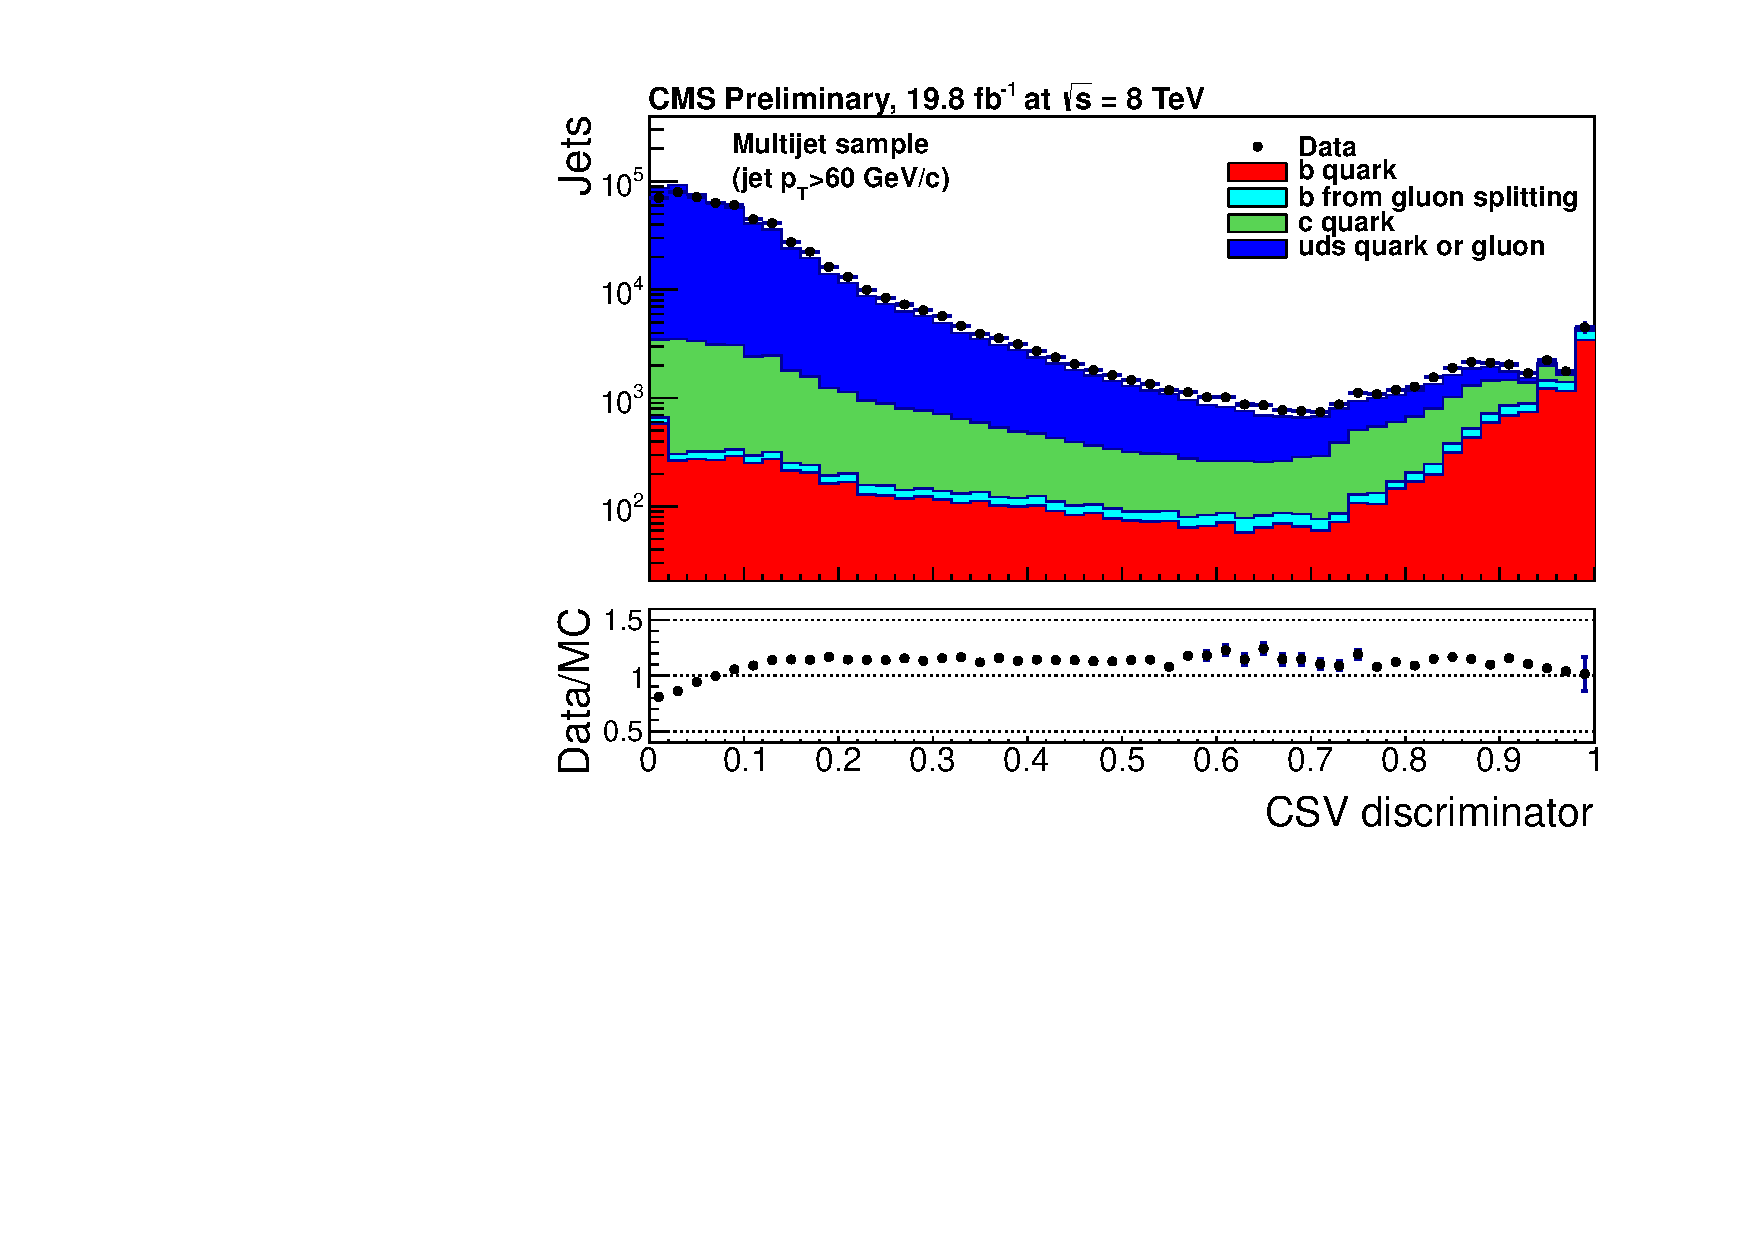
\includegraphics[width=\textwidth]{\figpath/Chapter4/b-tagging/Figure_006-e.pdf}
        \caption{}
        \label{fig:bDiscriminator_QCD}
    \end{subfigure}
    \begin{subfigure}[t]{0.48\textwidth}
        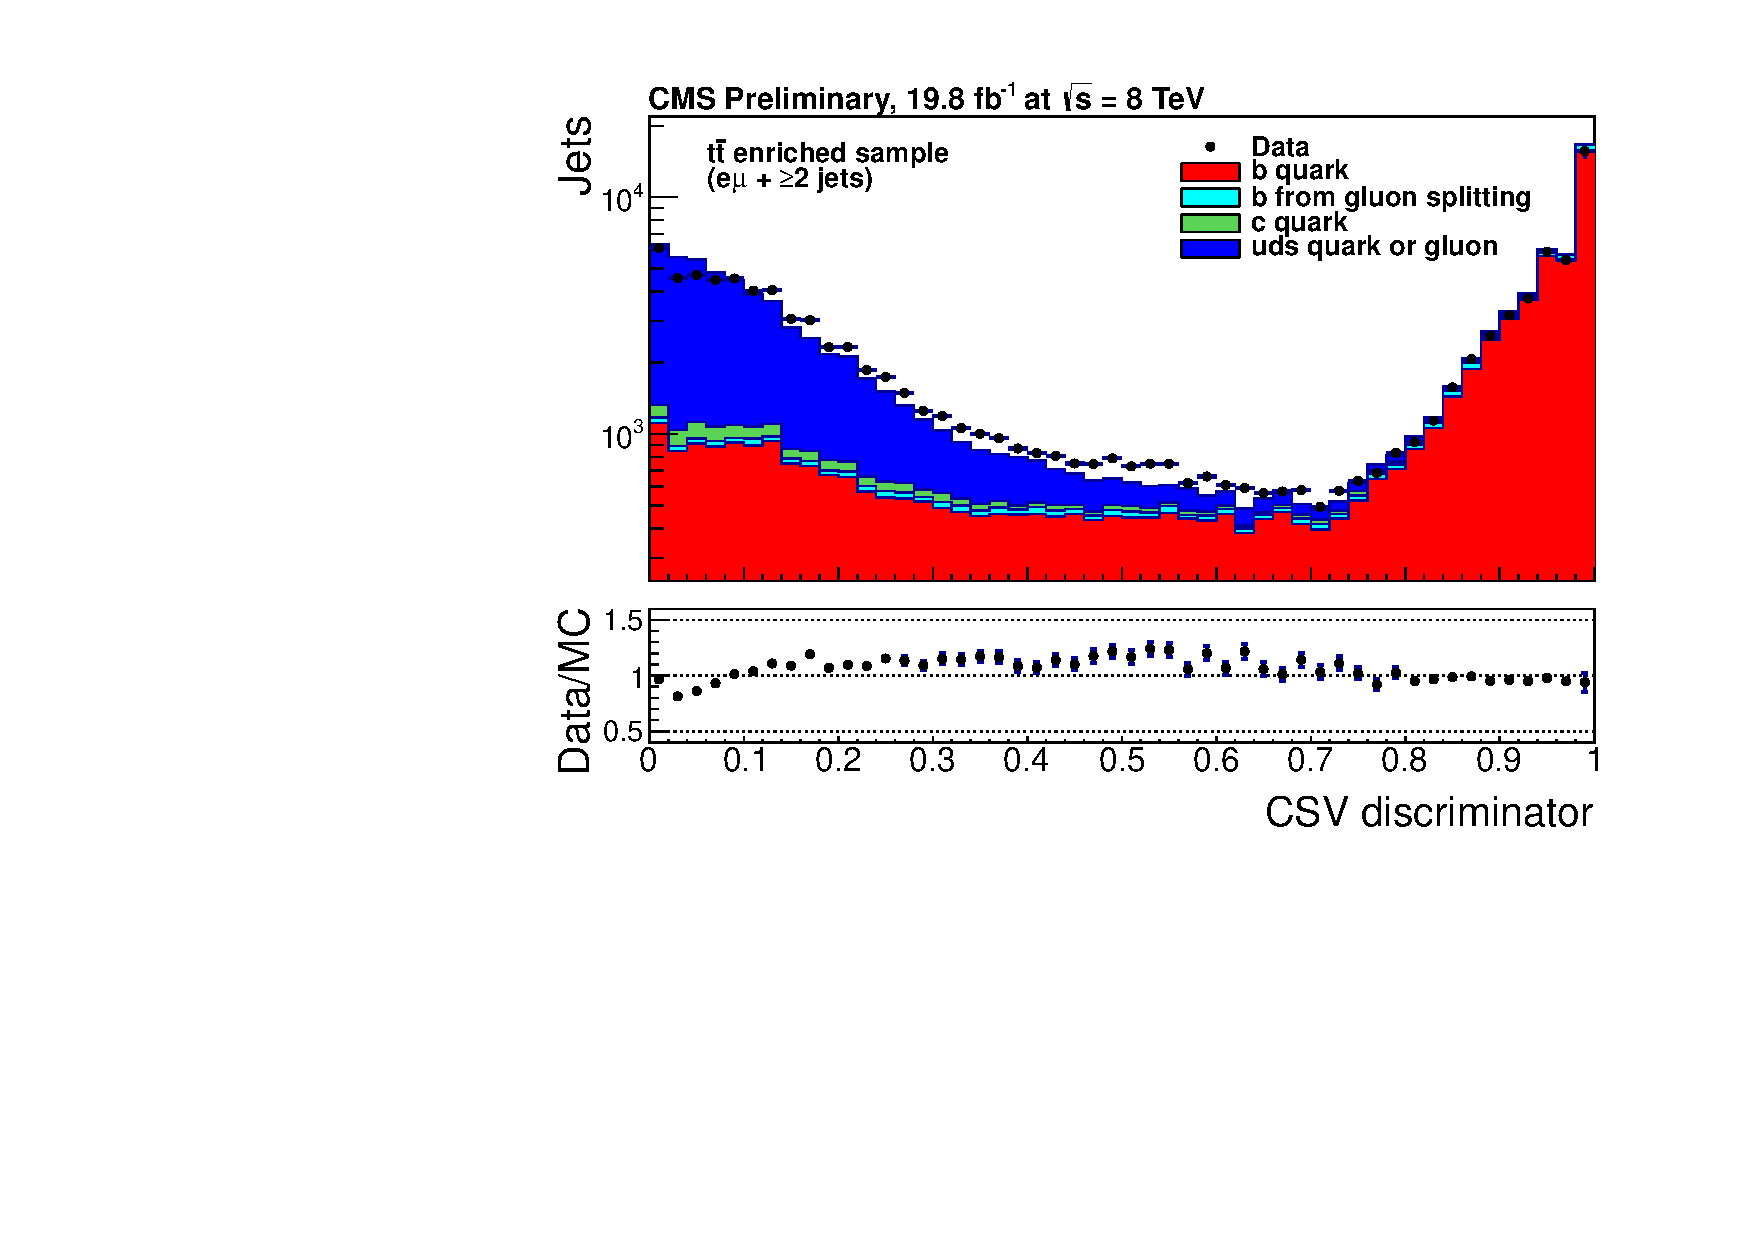
\includegraphics[width=\textwidth]{\figpath/Chapter4/b-tagging/Figure_006-f.pdf}
        \caption{}
        \label{fig:bDiscriminator_ttbar}
    \end{subfigure}
    \caption{The $d_{CSV}$ distribution in a (left) QCD dominated sample and (right) a \ttbar dominated sample~\cite{CMS-PAS-BTV-13-001}.}
    \label{fig:bDiscriminator}
\end{figure}

\begin{figure}[!hbt]
    \centering
    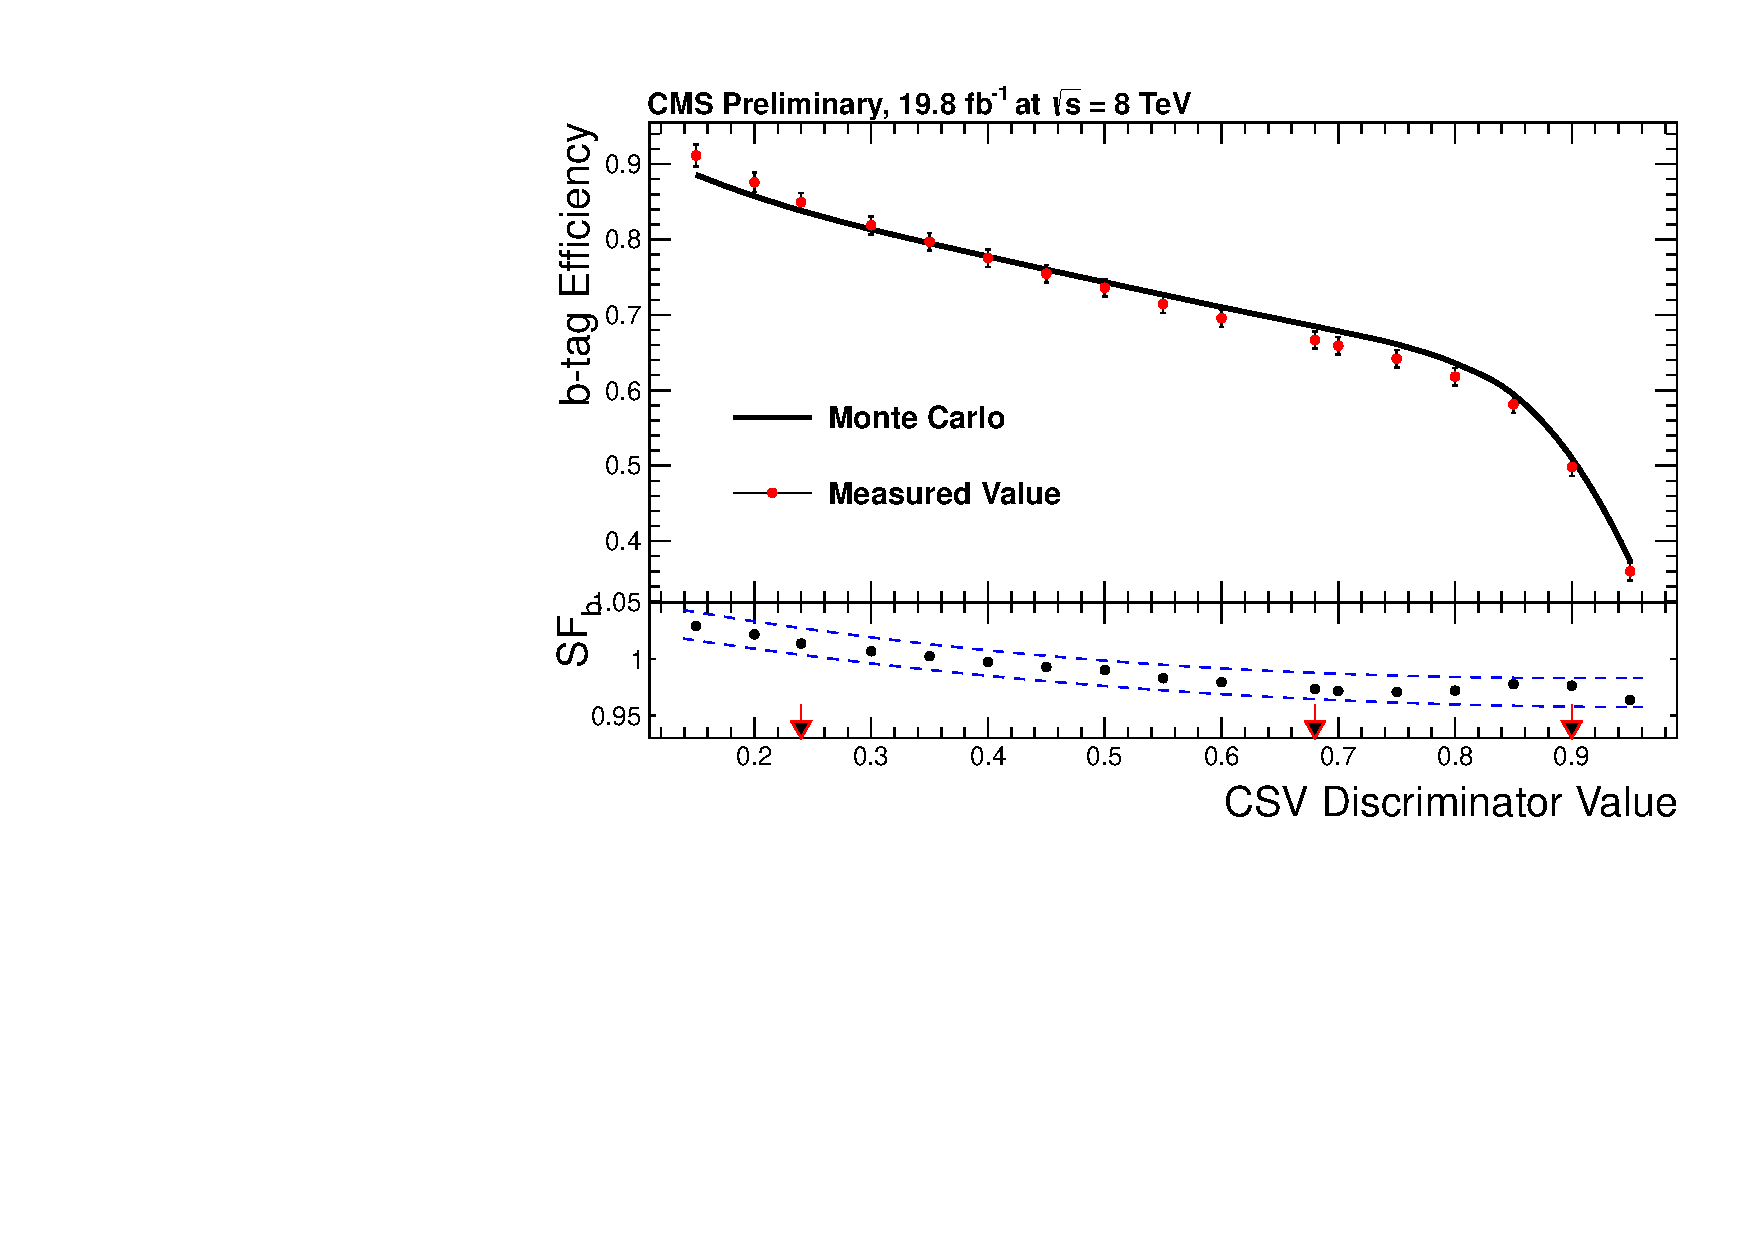
\includegraphics[width=0.95\textwidth]{\figpath/Chapter4/b-tagging/Figure_012-b.pdf}
    \caption{The b-tagging efficiency as a function of the CSV discriminator ($d_{CSV}$) value for both data and MC. The lower panel shows the ratio of the data and MC efficiencies and the arrows along the $x$-axis show the loose, medium, and tight working point values~\cite{CMS-PAS-BTV-13-001}.}
    \label{fig:bDiscriminator_efficiency}
\end{figure}

\section{Missing Transverse Energy}
\label{sec:MET}
%https://twiki.cern.ch/twiki/bin/view/CMSPublic/WorkBookMetAnalysis

While CMS is designed to detect as many particles as possible, some particles may be outside of the detector acceptance, may be mis-measured, or may simple not interact with the detection elements.
Examples of this are a particle which is beyond and $\eta$ of 5.0 or a neutrino, which will make it through the detector without ever interacting or a BSM particle which do not interact with the detector.
Furthermore, there may be additional particles in the event due to pileup which can can lead to fake \VETslash due to calorimeter thresholds and response nonlinearities.
Because the proton beams have near zero momentum in the $x$ and $y$ directions, only traveling in the $z$ direction, any imbalance in the momentum in the transverse plane indicates additional, missing, or mis-measured particles.
This imbalance is called missing transverse momentum and is the negative vector sum of \ptvec for all PF candidates in the event as seen in equation~\ref{eq:MET_uncorr_simple}.
The magnitude of this quantity is known as missing transverse energy and is represented as \ETslash~\cite{METperf2012}. A schematic of these two quantities is shown in fig.~\ref{fig:MET_schematic}.
\begin{equation}
\label{eq:MET_uncorr_simple}
\VETslashUncorr=-\sum_{i}{\vec{p}_{T}}^{\text{ }i}
\end{equation}

\begin{figure}[!hbt]
    \vspace*{-0.5cm}
    \centering
    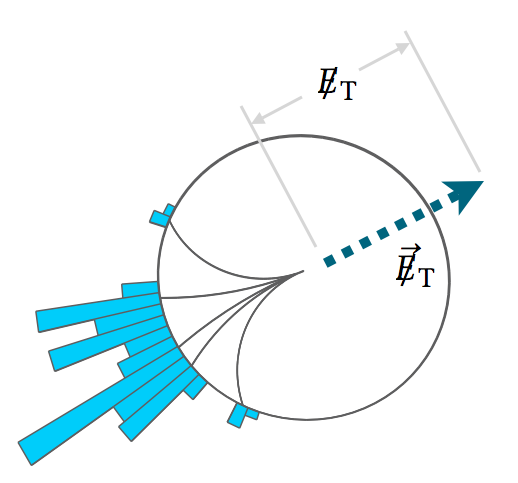
\includegraphics[width=0.95\textwidth]{\figpath/Chapter4/tai_20120616_met_schematic.png}
    \caption{A schematic of the \VETslash and \ETslash quantities~\cite{METAnalysis}.}
    \label{fig:MET_schematic}
\end{figure}

Because the \VETslash is affected by every \textit{visible} particle in the event, meaning particles which interact using the electromagnetic or strong forces, it is particularly sensitive to minimum energy thresholds in the calorimeters, inefficiencies and \pt thresholds in the tracker, and the non-linear, non-compensating response of the ECAL and HCAL.
While electrons and muons have a very good resolution and are typically measured correctly, composite objects like jets have a non-negligible affect on the \VETslash and the bias due to these effects can be reduced by correcting the jets and propagating those corrections to the \VETslash.
Unfortunately the corrections discussed in section~\ref{sec:jets} are applied to the composite object and not the the individual constituents\footnote{A method which is being actively worked on.}.
The jet energy corrections are therefore propagated to the \VETslash with the requirements that $f_{EM}<0.9$ and $\pt>10\gev$ so as to exclude electrons which may sometimes produce a non-genuine jet.
This type of correction is called Type-1 corrected \VETslash and is what is used in this analysis as a proxy for the undetected neutrino coming from the decay of one of the W boson.
%https://twiki.cern.ch/twiki/bin/view/CMS/METType1Type2Formulae
\begin{subequations}
    \label{eq:MET_type1}
    \begin{align}
\VETslashUncorr={}&-\sum_{i \in \textrm{jets}}\ptvecsub{i}-\sum_{i \notin \textrm{jets}}\ptvecsub{i} \label{eq:MET_uncorr_PFObjects}\\
={}&-\sum_{\textrm{jet}}\ptvecsubsup{jet}{uncorr.}-\sum_{i \notin \textrm{jets}}\ptvecsub{i} \label{eq:MET_uncorr_PFObjects_jets} \\
={}&-\sum_{\substack{\textrm{jet} \\ \ptvecsubsup{jet}{L123} > 10 \gev}}\ptvecsubsup{jet}{uncorr.}-\sum_{\substack{\textrm{jet} \\ \ptvecsubsup{jet}{L123} < 10 \gev}}\ptvecsubsup{jet}{uncorr.}-\sum_{i \notin \textrm{jets}}\ptvecsub{i} \label{eq:MET_uncorr_threshold}\\
\begin{split}\label{eq:MET_uncorr}
={}&-\sum_{\substack{\textrm{jet} \\ \ptvecsubsup{jet}{L123} > 10 \gev}}\ptvecsubsup{jet}{L1}-\sum_{\substack{\textrm{jet} \\ \ptvecsubsup{jet}{L123} > 10 \gev}}\left(\ptvecsubsup{jet}{uncorr.}-\ptvecsubsup{jet}{L1}\right)\\
&-\sum_{\substack{\textrm{jet} \\ \ptvecsubsup{jet}{L123} < 10 \gev}}\ptvecsubsup{jet}{uncorr.}-\sum_{i \notin \textrm{jets}}\ptvecsub{i}
\end{split}\\
\begin{split}\label{eq:MET_type1_final}
\VETslashsup{Type-1}={}&-\sum_{\substack{\textrm{jet} \\ \ptvecsubsup{jet}{L123} > 10 \gev}}\ptvecsubsup{jet}{L123}-\sum_{\substack{\textrm{jet} \\ \ptvecsubsup{jet}{L123} > 10 \gev}}\left(\ptvecsubsup{jet}{uncorr.}-\ptvecsubsup{jet}{L1}\right) \\
&-\sum_{\substack{\textrm{jet} \\ \ptvecsubsup{jet}{L123} < 10 \gev}}\ptvecsubsup{jet}{uncorr.}-\sum_{i \notin \textrm{jets}}\ptvecsub{i}
\end{split}
    \end{align}
\end{subequations}

Equation~\ref{eq:MET_uncorr_simple} shows the simplified and uncorrected model of \VETslash which can be broken into two categories, those particles which are contained in jets and those which are not.
This is shown in equation~\ref{eq:MET_uncorr_PFObjects}, but can be simplified further to equation~\ref{eq:MET_uncorr_PFObjects_jets} by noting that the first term is simply the sum of \pt for the uncorrected jets.
In equation~\ref{eq:MET_uncorr_threshold} the jets are further broken into two classes based on their corrected \pt and in equation~\ref{eq:MET_uncorr} the jets are broken into the pileup corrected jets term and a term for the pileup itself, where $\left(\ptvecsubsup{jet}{uncorr.}-\ptvecsubsup{jet}{L1}\right)$ is the additional energy due to pileup (offset).
Now that the \VETslash is fully broken down it can be corrected by replacing $\ptvecsubsup{jet}{L1}$ in the first term with $\ptvecsubsup{jet}{L123}$ to give equation~\ref{eq:MET_type1_final}.
This is a correction on the clustered energy in the event above a given threshold~\cite{METAnalysis}.

An additional modification to the \VETslash to remove a modulation in the $\varphi$ component is also used.
%and is discussed further in appendix~\ref{appendix:met_phi_corrections}.
\VETslash should be independent of $\varphi$ because the proton-proton collisions are rotationally symetric around the beam axis, so any asymmetry must be due to an error in the simulation or reconstruction.
However, we observed a sinasoidal modulation of period $2\pi$ in the \ETslashvarphi for both data and simulation after reconstruction, as can be seen in fig.~\ref{fig:METPhi_dataMC_Before}.
This effect can be caused by an anisotropic detector responses, inactive calorimeter cells, detector misalignment (for even one of the sub-detectors), or a displacement of the beam spot.
All of these will cause the same effect.

\begin{figure}[!hbt]
    \centering
    \begin{subfigure}[t]{0.48\textwidth}
      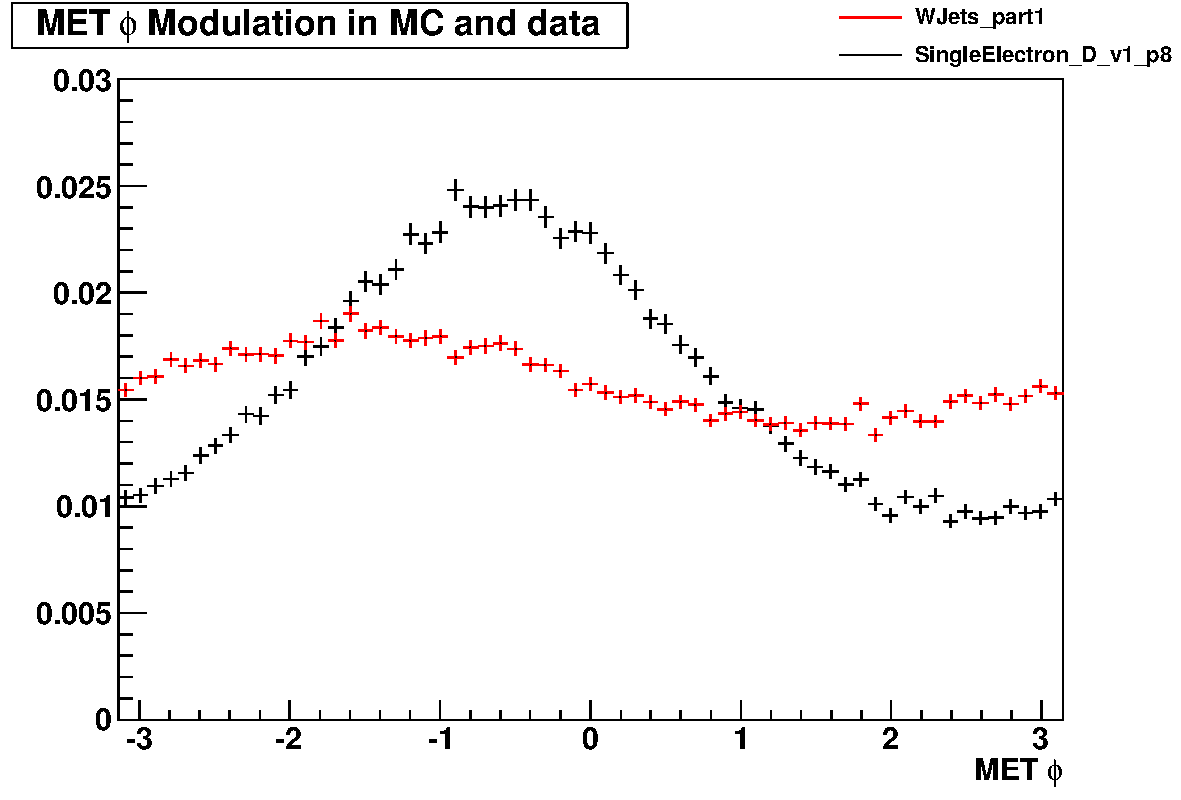
\includegraphics[width=\textwidth]{\figpath/Chapter4/METPhi_Before-eps-converted-to.pdf}
      \caption{}
      \label{fig:METPhi_dataMC_Before}
    \end{subfigure}
    \begin{subfigure}[t]{0.48\textwidth}
      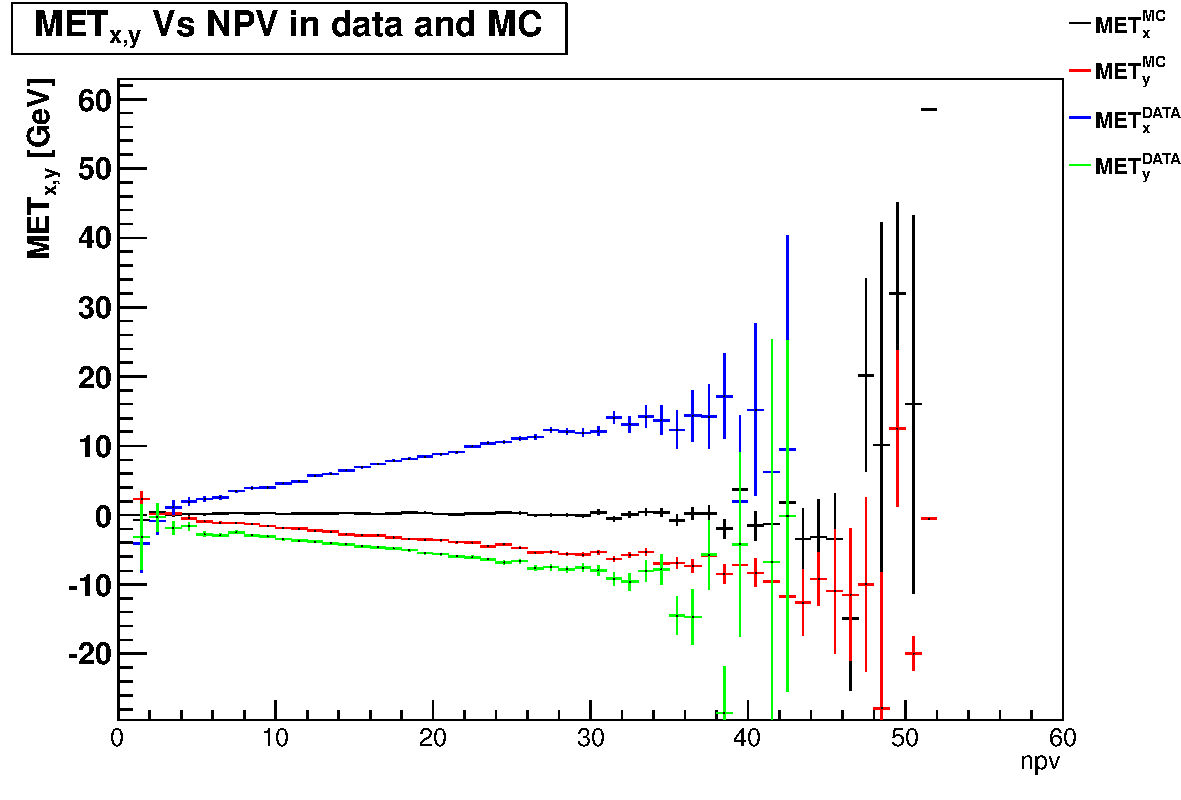
\includegraphics[width=\textwidth]{\figpath/Chapter4/METxyVsNPV_Before-eps-converted-to.pdf}
      \caption{}
      \label{fig:METxyVsNPV_Before}
    \end{subfigure}
    \caption{(a) Distribution of the \ETslashvarphi for data (black) and simulation (red). Only the \Wjets simulation is shown here, although all of the simulations suffer from the same modulation. (b) Distributions of \Eslashxy as a function of the number of primary vertices. The black and red markers represent the $x$ and $y$ distributions for simulation, respectively, while the blue and green markers are for data.}
    \label{fig:METPhi_Before}
\end{figure}

While the exact cause of the modulation might be unknown, we do know that the amplitude of the modulation increases linearly with the number of proton-proton interactions as each additional particle in the event will increase the $\varphi$ asymmetry.\footnote{Assuming the additional particles are created isotropically.}
The dependence on the number of primary vertices can be seen in fig.~\ref{fig:METxyVsNPV_Before}, which shows the $x$ and $y$ components of the \ETslash 4-vector as a function of the number of primary vertices.
Without first correcting this modulation, any cut on the \pt of the \ETslash would preferentially select events on a specific side of the detector.
Luckily, the amplitude of the modulation can be reduced by using the transformation in equation~\ref{eq:METPhi_transformation}.
\begin{equation}
\label{eq:METPhi_transformation}
{\vec{p}_{T}}^{\text{ }i}\rightarrow{\vec{p}_{T}}^{\text{ }i}-\vec{c}
\end{equation}
Thus the \VETslash becomes:
\begin{equation}
    \label{eq:METPhi}
    \begin{aligned}
\VETslashxy={}&-\sum_{i \in \textrm{all}}\left(\ptvecsub{i}-\vec{c}\right) \\
={}&-\sum_{i \in \textrm{all}}\ptvecsub{i}+\sum_{i \in \textrm{all}}\vec{c} \\
={}&\VETslashraw+n\vec{c} \\
={}&\VETslashraw+{\vec C}_{\mathrm{T}}^{\mathrm{xy}}
    \end{aligned}
\end{equation}
However, instead of applying this correction based on the number of particles, the correction is parameterized based on the number of vertices as a proxy for the number of particles. The correction as a function of the number of vertices is:
\begin{equation}
\label{eq:METPhi_correction}
{\vec C}_{\mathrm{T}}^{\mathrm{xy}}=\vec{c}_{A}+n_{vtx}\vec{c}_{B}
\end{equation}
where $\vec{c}_{A}$ and $\vec{c}_{B}$ are constant vectors and $n_{vtx}$ is the number of reconstructed primary vertices.

Practically this corrections is accomplished by fitting the distributions in fig.~\ref{fig:METxyVsNPV_Before} with a first order polynomial to obtain $\vec{c}_{A}$ and $\vec{c}_{B}$.
Those coefficients can be found in table~\ref.
Then we use equations~\ref{eq:METx_corr} and~\ref{eq:METy_corr}, which differ from equation~\ref{eq:METPhi} only due to the sign of the coefficients.
\begin{align}
E_{\mathrm{x}}^{\mathrm{corrected}}\hspace{-3.5em}/\kern3.1em ={}& E_{\mathrm{x}}^{\mathrm{RECO}}\hspace{-2.7em}/\kern2.4em - \left([0]_{\mathrm{x}}+[1]_{\mathrm{x}}{\cdot}\mathrm{N}_{\mathrm{PV}}\right) \label{eq:METx_corr}\\
E_{\mathrm{y}}^{\mathrm{corrected}}\hspace{-3.5em}/\kern3.1em ={}& E_{\mathrm{y}}^{\mathrm{RECO}}\hspace{-2.7em}/\kern2.4em - \left([0]_{\mathrm{y}}+[1]_{\mathrm{y}}{\cdot}\mathrm{N}_{\mathrm{PV}}\right) \label{eq:METy_corr}
\end{align} 
The results of this correction are shown in fig.~\ref{fig:METPhi_After}, where both the modulation in $\varphi$ and the slope as a function of N\textsubscript{PV} are gone.
From here we can place a cut on the \pt of the \VETslash object with biasing our selection.

\begin{table}[hbtp]\footnotesize
\centering
\begin{tabular}{l l l}
\hline
Coordinate & Parameter 0 & Parameter 1 \\
\hline
\multicolumn{3}{c}{\textbf{Data}} \\
\hline
$x$ & $2.0105E-01$ & $4.2663E-01$ \\
$y$ & $-9.1350E-01$ & $-2.3120E-01$ \\
\hline
\multicolumn{3}{c}{\textbf{MC}} \\
\hline
$x$ & $2.9059E-01$ & $-3.5293E-03$ \\
$y$ & $3.0183E-01$ & $-1.9974E-01$ \\
\hline
\end{tabular}
\caption{The fit parameters for the \VETslashvarphi corrections.}
\label{tab:METPhi_Correction_Coefficients}
\end{table}

\begin{figure}[!hbt]
    \centering
    \begin{subfigure}[t]{0.48\textwidth}
      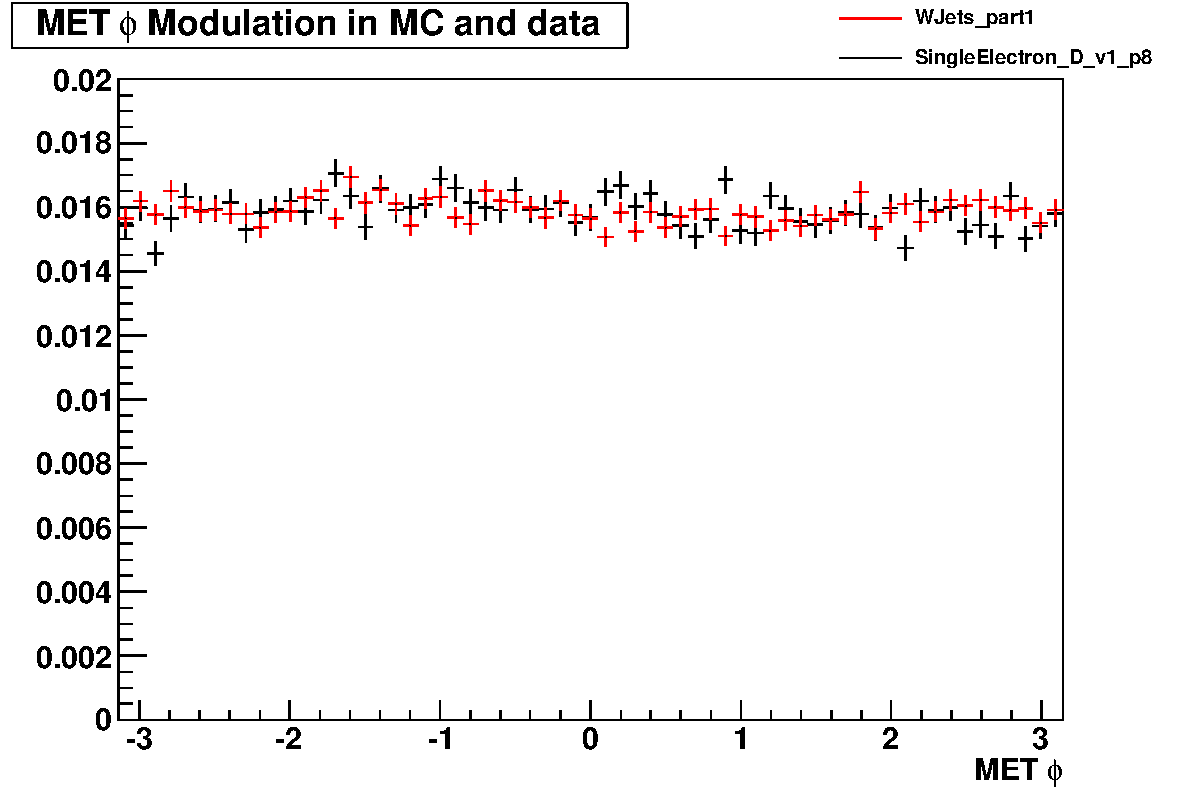
\includegraphics[width=\textwidth]{\figpath/Chapter4/METPhi_After-eps-converted-to.pdf}
      \caption{}
      \label{fig:METPhi_dataMC_After}
    \end{subfigure}
    \begin{subfigure}[t]{0.48\textwidth}
      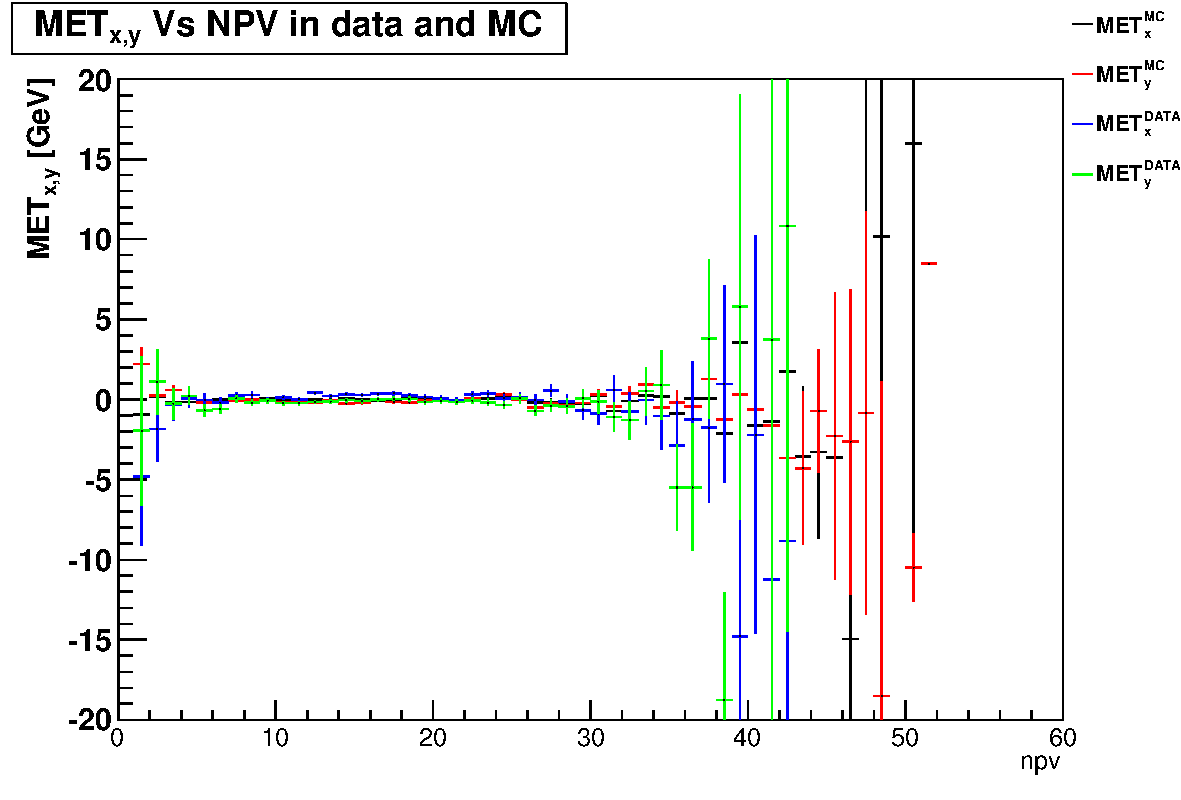
\includegraphics[width=\textwidth]{\figpath/Chapter4/METxyVsNPV_After-eps-converted-to.pdf}
      \caption{}
      \label{fig:METxyVsNPV_After}
    \end{subfigure}
    \caption{(a) Distribution of the \ETslashvarphi for data (black) and simulation (red) with the correction for the modulation applied. Only the \Wjets simulation is shown here, although all of the simulations suffer from the same modulation. (b) Distributions of \Eslashxy as a function of the number of primary vertices after the $\varphi$ modulation correction has been applied. The black and red markers represent the $x$ and $y$ distributions for simulation, respectively, while the blue and green markers are for data.}
    \label{fig:METPhi_After}
\end{figure}

In this analysis the resulting \ETslash is required to have at least 25\gev in order to reduce the QCD events making it through the selection process.
A pileup correction to the \VETslash was also available, but was not implemented in this analysis.
It is nevertheless discussed in appendix~\ref{appendix:type_zero_met}.
In addition to propagating the JEC to the \VETslash, CMS also filters events and or \VETslash contributions which might introduce noise from the calorimeters or beam halo~\cite{METperf2011}.
These filters are discussed further in appendix~\ref{appendix:met_filters}.

\section{Event Generation}
\label{sec:event_generation}

In the search for new physics, a signal will generally appear as a small deviation from the SM prediction.
In order to disentangle the SM background from a rare signal the SM and new physics prediction must be extremely accurate.
The predictions are samples made by Monte Carlo (MC) event generators which are broken up by physics process and final state and then recombined during the analysis~\cite{Siegert:2010cru,Mangano:2005dj,Dobbs:2004qw}.
These generators are able to simulate a full event (bunch crossing) at the parton level, which is nicely illustrated in fig.~\ref{fig:ttH_event}.
The image shows a $t\bar{t}h$ final state including final state gluons (QCD) and hadronization.
While the entire event from hard scatter production to hadronization cannot be described using perturbation theory, the hard process can be calculated using fixed order perturbation theory and matrix elements (ME).
The parton showers, red lines in fig.~\ref{fig:ttH_event}, then connect the hard process with the hadronization scale.
Phenomenological models are used to simulate the hadronization into stable particles and the underlying event (UE), which is the usually softer interactions by the constituents of the protons which did not take part in the hard scatter process.
Photon and gluon emission from the initial protons and final state partons, respectively called initial state radiation (ISR) and final state radiation (FSR), must also be simulated.

\begin{figure}[!hbt]
    \vspace*{-0.5cm}
    \centering
    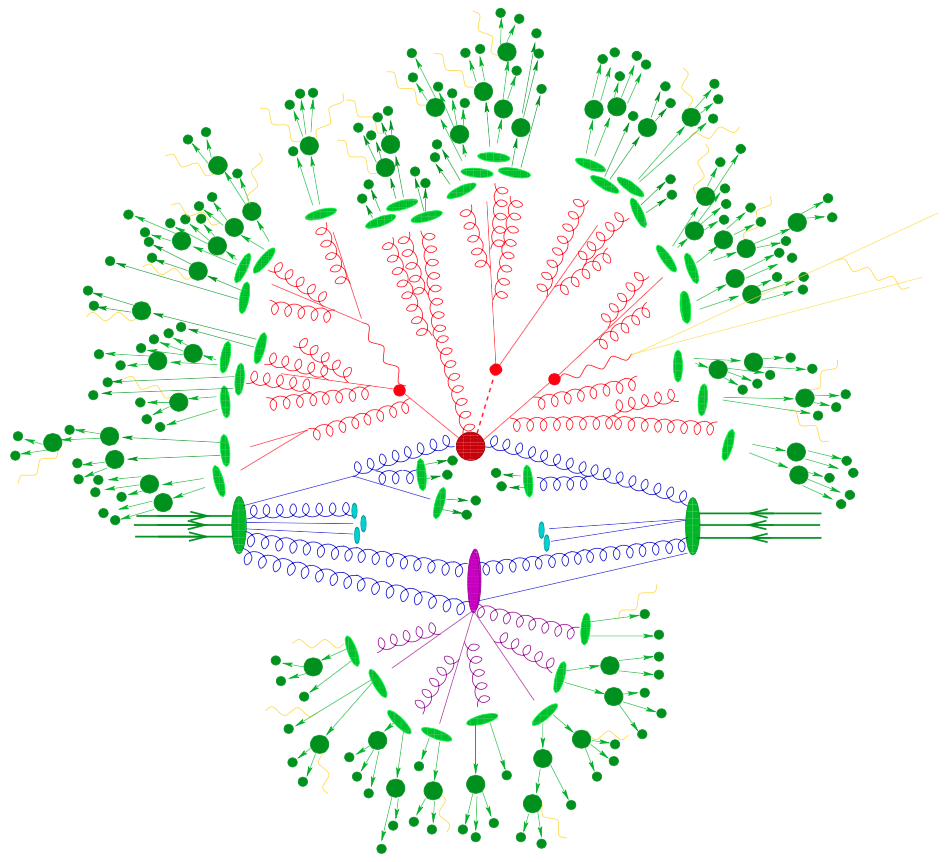
\includegraphics[width=0.95\textwidth]{\figpath/Chapter4/ttH_event.png}
    \caption{A graphical representation of a $t\bar{t}h$ event as seen by a MC event generator. The hard scatter interaction is represented by the red circle being produced by the two gluons coming of the incoming protons. The three small red dots represent the top quarks and the Higgs boson which then decay to additional hard QCD radiation. The underlying event is represented by the purple shapes and lines while the light green shapes are the final-state partons, which then hadronize and decay into the dark green circles. The yellow lines show the photon radiation which can occur at any state in the event generation process~\cite{Siegert:2010cru}.}
    \label{fig:ttH_event}
\end{figure}

Because protons are not elementary particles, it is important to discuss these interactions in terms of the partons inside the proton.
Hadrons, like the proton, are made up of valence quarks, sea quarks, and gluons\footnote{More precisely, protons are a bound state of two up quarks and a down quark.}.
In essence, the simulation of a proton-proton hard scatter interaction is the calculation of a cross section for an N-particle final state, seen in equation~\ref{eq:event_generation_cross_section}, where $a$ ($b$) is a parton carrying a fraction of the momentum $x_{a}$ ($x_{b}$) for hadron $A$ ($B$).
\begin{equation}
\label{eq:event_generation_cross_section}
\sigma_{N}^{AB}\left(s\right)=\int dx_{a}dx_{b}f_{a}\left(x_{a},\mu^{2}\right)f_{b}\left(x_{b},\mu^{2}\right)\hat{\sigma}_{N}^{ab}\left(\hat{s},\mu^{2}\right)
\end{equation}
The parton distribution function (PDF) of the form $f_{a,b}\left(x_{a,b},\mu^{2}\right)$ gives the probability density of finding such a parton with momentum fraction $x_{a,b}$ renormalized to scale $\mu^{2}$.
PDFs cannot be obtained using perturbative nor lattice QCD calculations.
Instead they are measured within the resolution of the existing experiments.
CMS makes use of the Martin-Stirling-Thorne-Watt (MSTW)~\cite{Martin:2009iq} and Coordinated Theoretical-Experimental Project on QCD (CTEQ) PDFs.
Fig.~\ref{fig:mstw} shows the NLO MSTW PDFs calculated for two different momentum scales.
Other terms include the center-of-mass energy of the interaction $\sqrt{\hat{s}}=\sqrt{x_{a}x_{b}s}$ where $\sqrt{s}$ is the center-of-mass energy of the proton-proton system and $\hat{\sigma}_{ab\rightarrow{X}}\left(\hat{s},\mu^{2}\right)$, which is the cross section for having a given set of initial state partons. The full form of the partonic cross section is given by 
\begin{equation}
\begin{split}\label{eq:event_generation_partonic_cross_section}
\hat{\sigma}_{N}^{ab}=\int_{cuts}d\hat{\sigma}_{N}^{ab}={}&\frac{\left(2\pi\right)^{4}S}{4\sqrt{\left(p_{1}{\cdot}p_{2}\right)^{2}-m_{1}^{2}m_{2}^{2}}}\times \\ &\int_{cuts} \left[\prod_{i=1}^{N}\frac{d^{3}q_{i}}{\left(2\pi\right)^{3}2E_{i}}\right]\delta^{4}\left(p_{1}+p_{2}-\sum_{i}^{N}q_{i}\right)|\mathcal{M}_{p_{1}p_{2}\rightarrow\{\vec{q}\}}^{ab}|^{2}
\end{split}
\end{equation}
where $p_{i}$ are the four-momenta of the incoming partons, $q_{i}$ and $E_{i}$ are the outgoing particle four-momenta and energies, $S$ is the product of $1/j!$ for j identical particles in the final state, and $\mathcal{M}_{p_{1}p_{2}\rightarrow\{\vec{q}\}}^{ab}$ is the ME associated to the kinematic configuration $p_{1}p_{2}\rightarrow\{\vec{q}\}$ with initial partons $a$ and $b$~\cite{Siegert:2010cru,Griffiths2008}.
In order to evaluate the parton level ME the event generator must either have the ME hard coded or it must be able to compute all of the Feynman diagrams associated with a given process.
A good example of this type of calculation can be found in Table 1.1 of~\cite{Siegert:2010cru}.
While the number of diagrams for a $2\rightarrow2$ or $2\rightarrow3$ process is limited and can be built and computed automatically, the problem becomes much more difficult for next to leading order (NLO) computations as the number of diagrams grows factorially~\cite{Kurihara:2002ne}.
The growth of the number of diagrams can be seen in fig.~\ref{fig:NumberOfDiagrams}.
In many cases the LO MEs and PDFs are used to generate events and a K-factor is used to scale the events to their NLO or NNLO predictions.
Besides computing the MEs, the the multi-dimensional phase space integration is quite complicated and requires the use of Monte-Carlo integration techniques~\cite{MonteCarloMethods}.

\begin{figure}[!hbt]
    \vspace*{-0.5cm}
    \centering
    \includegraphics[width=0.95\textwidth]{\figpath/Chapter4/mstw2008nlo68cl_allpdfs.png}
    \caption{The MSTW PDFs calculated to NLO as a function of the momentum fraction for two different interaction momentum scales $Q^{2}$. In the case of synchrotron collisions $Q^{2}$ is the square of the total four-momentum of the proton-proton interaction. The right plot shows the momentum scale more commonly found at the LHC~\cite{Martin:2009iq}.}
    \label{fig:mstw}
\end{figure}

\begin{figure}[!hbt]
    \vspace*{-0.5cm}
    \centering
    \includegraphics[width=0.95\textwidth]{\figpath/Chapter4/NumberOfDiagrams.png}
    \caption{The number of diagrams which must be calculated to fully calculate the $gg\rightarrow{ng}$ amplitude~\cite{Siegert:2010cru}.}
    \label{fig:NumberOfDiagrams}
\end{figure}

The parton shower takes the partons created by the hard process and UE and perturbatively evolves them down to the hadronization scale, at which point they form colorless hadrons.
The partons are initially produced at a scale $t'$ and the parton shower determines the scale $t<t'$ at which the parton should branch into two daughter particles, selecting the kinematics and flavors of those new particles.
This process continues recursively and only ceases once the hadronization scale is reached, $\mathcal{O}\left(\gev\right)$, where $\alpha_{s}$ becomes large and perturbative methods are no longer applicable. 
Generators make use of any number of phenomenological models, including the Lund string model~\cite{ANDERSSON198331,Andersson:1997hs} and the cluster hadronization model~\cite{WEBBER1984492,Winter:2003tt}, to turn this list of colored partons into colorless hadrons.
No matter the model used, the hadrons which result from these models are often unstable and will forced to decay into stable hadrons, which are defined to have a mean lifetime above a given threshold as defined by the experiment.

Various generators are used in this analysis, each with their own benefits and drawbacks. \textsc{pythia}~\cite{1126-6708-2006-05-026} is a general purpose event generator capable of handling many $2\rightarrow1,\text{ }2,\text{ }3$ processes.
It is capable of handling all of the needed generation steps including generating the hard scatter process, parton showering to the leading log (LL) level, hadronization, and the UE simulation. \textsc{pythia} makes use of the Lund string model for hadronization and describes the UE as additional, but not quite independent perturbative $2\rightarrow2$ scatterings. 
Another generator used is \textsc{Mad}\textsc{Graph}~\cite{Alwall:2014hca}, which more accurately simulates hard parton emission (i.e. ISR and FSR), but must be interfaced with \textsc{pythia} for showering soft and collinear radiation.
The \textsc{POWHEG}~\cite{Nason:2004rx,Alioli:2010xd} generator uses NLO matrix elements and PDFs and then matches this with a modified shower simulation.
Both \textsc{Mad}\textsc{Graph} and \textsc{POWHEG} are interfaced with \textsc{pythia} for hadronization.
For more accurate tau lepton decays CMS often uses the \textsc{tauola}~\cite{WAS200196} software package.

\section{Detector Simulation}
\label{sec:detector_simulation}

Event generation simulates the particle kinematics for a given event, but doesn't examine how the particles will interact with the detector and it's constituent materials or how the readout electronics will behave.
To simulate the response of the CMS detector, the generators are interfaced with a sophisticated detector simulation based on the \textsc{Geant4}~\cite{geant4nim,geant4ieee} software package, which takes into account the exact detector geometry as well as all materials used.
The alignment, calibration, and other conditions which may change over time are periodically checked and are stored in a database.
These conditions are used both for offline simulation and reconstruction as well as for online activities.
The final state particles from the event generator are sent to the detector simulation, which tracks the particles as they move through the detector depositing energy into what are called simulated hits (SimHits).
While the models of electromagnetic interactions are extremely precise, the hadronic interactions have a greater uncertainty associated with them.
The simulation goes through the data acquisition process, event simulating the responses of the photodetectors and readout electronics.
The resulting information is then analyzed by the same reconstruction process that the real data goes through and is stored using the ROOT~\cite{Brun199781} software library.
%%!TEX root = ../TAMUTemplate.tex
%%%%%%%%%%%%%%%%%%%%%%%%%%%%%%%%%%%%%%%%%%%%%%%%%%%
%
%  New template code for TAMU Theses and Dissertations starting Fall 2016.
%
%  Author: Sean Zachary Roberson
%	 Version 3.16.09
%  Last updated 9/12/2016
%
%%%%%%%%%%%%%%%%%%%%%%%%%%%%%%%%%%%%%%%%%%%%%%%%%%%
%%%%%%%%%%%%%%%%%%%%%%%%%%%%%%%%%%%%%%%%%%%%%%%%%%%%%%%%%%%%%%%%%%%%%%
%%                           SECTION V
%%%%%%%%%%%%%%%%%%%%%%%%%%%%%%%%%%%%%%%%%%%%%%%%%%%%%%%%%%%%%%%%%%%%%



\chapter{\texorpdfstring{\uppercase {Higgs Analysis}}{Higgs Analysis}}
\label{ch:analysis}

Data collected by the CMS detector at the LHC is analyzed for the presence of a Higgs boson decaying to the \lvjj final state.
Signal and background Monte Carlo (MC) samples are used to study the efficacy of various object and event selection criteria.
While the signal samples are fully MC based, some of the background samples use data-driven techniques, which will be discussed later in this chapter.
The matrix element probabilities for an event final state being created by a specific diagram are computed.
Several multivariate techniques are studied and used to distinguish between signal-like and background-like events.
We use the discriminator outputs from these multivariate classifiers to set limits on the SM \HWW cross section.

\section{Data and Monte Carlo Samples}

%The following sections will describe the datasets collected by CMS as well as the MC samples used in this analysis.

\subsection{Data}
\label{sec:data}

As mentioned previously, this analysis makes use of the full 2012 CMS dataset of 8\tev data.
Fig.~\ref{fig:int_lumi_per_day} shows the cumulative delivered, recorded, and validated luminosity versus time.
Only fully validated data, where both the LHC and CMS are completely operational, are use used for CMS analyses~\cite{LumiPublic}.
Table~\ref{tab:dataSamples} shows the data samples used for this analysis, which corresponds to $\sim$19.2\fbinv.
The datasets are split by the two HLT paths used, one which selects for a single high \pt electron and one for a single high \pt muon.
These two separate PDs correspond to the HLT\_Ele27\_WP80\_v* and HLT\_IsoMu24\_eta2p1\_v* trigger paths, respectively.
The HLT\_Ele27\_WP80\_v* path requires a reconstructed electron with \ptgt{27}\gev along with several other criteria grouped into a working point with 80\% efficiency of selecting true electrons.
The HLT\_IsoMu24\_eta2p1\_v* criteria requires an isolated, reconstructed muon with \ptgt{24}\gev within \absetalt{2.1}.
The luminosities listed in the table are associated with a 2.6\% uncertainty as specified in~\cite{CMS-PAS-LUM-12-001} and were collected using the HF luminosity measurements~\cite{CMS-PAS-LUM-13-001}.

\begin{figure}[!hbt]
    \centering
    \includegraphics[width=0.95\textwidth]{\figpath/Chapter5/int_lumi_per_day_cumulative_pp_2012_SummerConf.png}
    \caption{Cumulative day-by-day integrated luminosity in 2012 delivered by the LHC (blue), recorded by CMS (dark orange), and validated for physics use (light orange)~\cite{DataQuality}.}
    \label{fig:int_lumi_per_day}
\end{figure}

\begin{table}[hbtp]\footnotesize
\centering
\begin{tabular}{l l l}
\hline
 Dataset & Run Range & Integrated Luminosity \\
\hline
/SingleMu/Run2012A-13Jul2012-v1/AOD & 190645-196531 & 0.809$\fbinv$ \\
/SingleMu/Run2012A-recover-06Aug2012-v1/AOD & 190782-190949 & 0.082$\fbinv$ \\
/SingleMu/Run2012B-13Jul2012-v1/AOD & 193834-196531 & 4.383$\fbinv$ \\
/SingleMu/Run2012C-24Aug2012-v1/AOD & 198022-198523 & 0.489$\fbinv$ \\
/SingleMu/Run2012C-PromptReco-v2/AOD & 194631-203002 & 6.285$\fbinv$ \\
/SingleMu/Run2012D-PromptReco-v1/AOD & 194480-208686 & 7.231$\fbinv$ \\
{\bf Total SingleMu} & {\bf 190645--208686} & {\bf 19.279$\fbinv$} \\
\hline
/SingleElectron/Run2012A-13Jul2012-v1/AOD & 190645-196531 & 0.809$\fbinv$ \\
/SingleElectron/Run2012A-recover-06Aug2012-v1/AOD & 190782-190949 & 0.082$\fbinv$ \\
/SingleElectron/Run2012B-13Jul2012-v1/AOD & 193834-196531 & 4.336$\fbinv$ \\
/SingleElectron/Run2012C-24Aug2012-v1/AOD & 198022-198523 & 0.489$\fbinv$ \\
/SingleElectron/Run2012C-PromptReco-v2/AOD & 194631-203002 & 6.194$\fbinv$ \\
/SingleElectron/Run2012D-PromptReco-v1/AOD & 194480-208686 & 7.238$\fbinv$\\
{\bf Total SingleElectron} & {\bf 190645--208686} & {\bf 19.148$\fbinv$} \\
\hline
\end{tabular}
\caption{The datasets analyzed for this analysis.}
\label{tab:dataSamples}
\end{table}

\subsection{Monte Carlo}

This analysis makes use of MC simulation to study the background processes which have similar final states to that of the \HWWlvjj signal.
Both the kinematic distributions and the final yields are extracted from these samples.
The MC simulation is used for all backgrounds except for the multijet process, where a data-driven approach is used instead.
The process of developing this sample is described in detail in the section~\ref{sec:QCD_data-driven_sample}.
The signal sample kinematics and yields are also taken from MC.
Tables~\ref{tab:SignalSamples} and~\ref{tab:bkgSamples} list all of the MC sample for the Higgs signals and SM background processes, respectively.
The SM background and volunteer signal samples are centrally produced by the CMS collaboration.
The \ggH samples were produced specifically for this analysis.
All of the samples, regardless of who produced them, are stored in a database called the Data Aggregation System (DAS) and organized by the ``Dataset Name'' field.
The backgrounds were modeled by MC samples generated with \textsc{MadGraph}~\cite{Alwall:2014hca} and \textsc{pythia6}~\cite{1126-6708-2006-05-026}. 
The signal MC samples were also generated by \textsc{pythia6}.
Tables~\ref{tab:bkgSamples} and~\ref{tab:SignalSamples} list all of the MC for the Higgs signal and SM background processes, respectively.

\begin{sidewaystable}[hbtp]\footnotesize
\centering
\begin{tabular}{l p{0.50\textwidth} l l}
\hline
\multicolumn{4}{c}{Signal Processes} \\
\hline
Production \& Decay Modes & Dataset Name & Cross Section [\unit{pb}] & BR\\  \hline
\ggH; $\MH=\text{125}\gev$, \HWWlvjj & /LQ-ggh125\_BIG\_SIM\_ggH125\_part1/aperloff-LQ-ggh125\_AODSIM\_Summer12\_START53\_V7E-{\newline}768a14b04b0ac2af0d20e6783fbdb759/USER & 19.27 & 0.0947 \\
  & /LQ-ggh125\_BIG\_GEN\_part2/aperloff-LQ-ggh125\_BIG\_RECO\_part2-33e909ff21293ad9fa8564de2959fe54/USER & 19.27 & 0.0947\\
  & /LQ-ggh125\_BIG\_GEN\_part3/aperloff-LQ-ggh125\_BIG\_RECO\_part3-33e909ff21293ad9fa8564de2959fe54/USER & 19.27 & 0.0947\\
  & /LQ-ggh125\_Part6\_SIM/goodell-LQ-qqh125\_RECO\_Part6-33e909ff21293ad9fa8564de2959fe54/USER & 19.27 & 0.0947\\
  & /LQ-ggh125\_Part7\_SIM/goodell-LQ-qqh125\_RECO\_Part7-33e909ff21293ad9fa8564de2959fe54/USER & 19.27 & 0.0947\\
  & /LQ-ggh125\_Part8\_GENSIM/goodell-LQ-ggh125\_Part8\_RECO-33e909ff21293ad9fa8564de2959fe54/USER & 19.27 & 0.0947\\
\qqH; $\MH=\text{125}\gev$, \HWWlvjj & /LQ-vbf125\_GENSIM/ajkumar-LQ-qqh125\_AODSIM\_Summer12\_{\newline}START53\_V7A-c8f8ed334db8a7d6f56c62266b1dfa5b/USER & 1.578 & 0.0947\\
\WH, \ZH, \ttH; $\MH=\text{125}\gev$, \HWW, inclusive & /WH\_ZH\_TTH\_HToWW\_M-125\_8TeV-pythia6 & 1.249 & 0.215\\\hline
\multicolumn{4}{c}{Non signal Higgs Production} \\ \hline
\WH, \ZH, \ttH; $\MH=\text{125}\gev$, \HZZ, inclusive & /WH\_ZH\_TTH\_HToZZ\_M-125\_8TeV-pythia6 & 1.249 & 0.0264\\
\WH; $\MH=\text{125}\gev$, \Hbb, \Wlv & /WH\_WToLNu\_HToBB\_M-125\_8TeV-powheg-herwigpp & 0.7046 & 0.1879\\
\ttH; $\MH=\text{125}\gev$, \Hbb & /TTH\_HToBB\_M-125\_8TeV-pythia6 & 0.1293 & 0.577\\
\hline
\end{tabular}
\caption{List of signal datasets and cross sections. All of the centrally produced sample names are followed by /Summer12\_DR53X-PU\_S10\_START53\_V7A-v1/AODSIM.}
\label{tab:SignalSamples}
\end{sidewaystable}

\begin{sidewaystable}[hbtp]\footnotesize
\centering
\begin{tabular}{l p{0.65\textwidth} l}
\hline
\multicolumn{3}{c}{Background Processes} \\
\hline
Process & Dataset Name & Cross Section [\unit{pb}] \\
\hline
\Wjets & /WJetsToLNu\_TuneZ2Star\_8TeV-madgraph-tarball & 37509 \\
\ttbar & /TTJets\_MassiveBinDECAY\_TuneZ2star\_8TeV-madgraph-tauola & 225.197 \\
\Zjets & /DYJetsToLL\_M-50\_TuneZ2Star\_8TeV-madgraph-tarball & 3387.6 \\
\WW & /WW\_TuneZ2star\_8TeV\_pythia6\_tauola & 54.838 \\
\WZ & /WZ\_TuneZ2star\_8TeV\_pythia6\_tauola & 33.21 \\
\ZZ & /ZZ\_TuneZ2star\_8TeV\_pythia6\_tauola & 17.654 \\
$\cPqt\rightarrow\cPqb\ell\nu$ (\cPqs-channel) & /T\_s-channel\_TuneZ2star\_8TeV-powheg-tauola & 3.79 \\
$\cPqt\rightarrow\cPqb\ell\nu$ (\cPqt-channel) & /T\_t-channel\_TuneZ2star\_8TeV-powheg-tauola & 56.4 \\
$\cPqt\rightarrow{X}$ (\cPqt\W-channel) & /T\_tW-channel-DR\_TuneZ2star\_8TeV-powheg-tauola & 11.1 \\
$\cPaqt\rightarrow\cPqb\ell\nu$ (\cPqs-channel) & /Tbar\_s-channel\_TuneZ2star\_8TeV-powheg-tauola & 1.76 \\
$\cPaqt\rightarrow\cPqb\ell\nu$ (\cPqt-channel) & /Tbar\_t-channel\_TuneZ2star\_8TeV-powheg-tauola & 30.7 \\
$\cPaqt\rightarrow{X}$ (\cPqt\W-channel) & /Tbar\_tW-channel-DR\_TuneZ2star\_8TeV-powheg-tauola & 11.1 \\
QCD (\Pe-channel) & See table~\ref{tab:dataSamples} for a list of SingleElectron datasets & N/A \\
QCD (\Pmu-channel) & See table~\ref{tab:dataSamples} for a list of SingleMu datasets & N/A \\
\hline
\end{tabular}
\caption{List of background MC datasets and cross sections used in the analysis. Every dataset name is followed by /Summer12\_DR53X-PU\_S10\_START53\_V7A-v1/AODSIM. In addition to v1, this analysis also uses v2 of the \Wjets sample.}
\label{tab:bkgSamples}
\end{sidewaystable}

The \ttbar, \Wjets, and \Zjets SM background samples are generated using \textsc{Mad}\textsc{Graph} v5.1.3.30~\cite{Alwall:2014hca}.
The \ttbar sample is inclusive, meaning that it includes all decay modes of the \W boson coming from the top decay.
The \Wjets and \Zjets samples are also inclusive, but in this case it means that in addition to the leptonic decay of the boson there are any number of final state jets.
The single top quark samples are modeled using the \textsc{POWHEG} 1.0 r138 ~\cite{POWHEG2,POWHEG:singlet,POWHEG:singletW} generator.
The diboson processes use the \textsc{pythia} v6.4.24 generator~\cite{1126-6708-2006-05-026}.
The cross sections for the \ttbar and single top quark processes are calculated at next-to-next-to-leading logarithmic (NNLL) accuracy~\cite{TOPCrossSec} while the inclusive \Wjets and \Zjets processes are calculated at next-to-next-to-leading order (NNLO) accuracy~\cite{FEWZ}.
The diboson cross sections are calculated at next-to-leading order (NLO) accuracy~\cite{MCFM}.

The \HWW signal samples are generated with \textsc{pythia} v6.4.24~\cite{1126-6708-2006-05-026}, where one \W is required to decay leptonically while the other is required to decay hadronically.
The cross sections for the Higgs production are calculated at NNLL QCD and NLO EW accuracies.
The calculations for gluon-gluon fusion and VBF production cross sections use the complex-pole-scheme (CPS) while the associated production cross section are calculated with the zero-width-approximation (ZWA)~\cite{Heinemeyer:2013tqa}.
These samples were privately produced because the centrally produces samples did not include enough events and had large statistical fluctuations.

\subsection{Multijet-QCD Background}
\label{sec:QCD_data-driven_sample}

It is well known that the QCD process is difficult to model to the desired level of accuracy.
Additionally, the event selection in this analysis requires two isolated jets and an isolated lepton, which vastly reduces the number of QCD MC events that pass the selection criteria.
Although the probability to mis-reconstruct a jet as a lepton is fairly low, the production cross section for the multijet process is extremely high and thus cannot be ignored.
When using the MC samples we are left with a statistically limited sample that is almost useless for describing this background.

Rather than relying on MC for the QCD background sample, a data-driven sample was created by using the same trigger requirements as the data, but removing the isolation requirement for the lepton and inverting the lepton particle flow isolation cut during selection.
The main idea of the method is to utilize differences in lepton identification properties that separate prompt, isolated leptons from \W and \Z decays, also known as ``real leptons,'' from non-prompt, non-isolated leptons, also known as ``fake leptons.''
The normal signal selection requires an isolated lepton, without other particles around it, to limit this sort of ``fake lepton,'' but this is exactly the type of property we want to select for when forming a QCD sample from data.
This process provides a completely orthogonal sample of QCD events from data that won't, and shouldn't be used for signal extraction.
Since we make use of the entire 2012 dataset\footnote{The QCD events are scaled slightly to account for failed jobs (missing luminosity) during processing.}, we end up with statistically rich samples containing lots of mis-identified leptons.

A complete description of the event selection will be discussed in section~\ref{ch:event_selection}, but here I will just talk about the isolation requirements.
The loosest lepton PF isolation requirement used to determine the signal region is $\pfiso<0.2$, which is used to veto on ``loose'' or questionable leptons.
The assumption is that any lepton with $\pfiso>0.2$ is a mis-reconstructed lepton coming from QCD.
For electrons we must also turn off the MVA-based identification requirements as they are stringent enough that they won't allow for any fake leptons to pass our selection.
As mentioned before, the electrons must still pass the ``HLT\_Ele27\_WP80\_v*'' electron trigger used for the data containing our signal.
On the other hand, the muon trigger is changed to be ``HLT\_Mu24\_eta2p1\_v*'' to remove the isolation requirement that was included in the trigger used to select for the signal.

In order to gain greater separation from the signal selection to ensure as little non-QCD contamination as possible, we actually use a minimum isolation requirement of $\pfiso>0.3$.
We also put an upper limit on the PF isolation value to keep the sample from having a bias towards high nPV values.
For electrons the upper limit was 0.7 and for muons it was 2.0.
The $1\sigma$ systematic uncertainty bands for electrons (muons) were selected to be $0.2<\pfiso<0.3$ on the low side and $>$0.7 (2.0) for the high side
Fig.~\ref{fig:PFIsolation} shows the pf isolation values contained in the electron multijet and data samples as a function of $\eta$.

\begin{figure}[!hbt]
    \centering
    \begin{subfigure}[t]{0.475\textwidth}
        \includegraphics[width=\textwidth]{\figpath/Chapter5/pfIsoVsEta_DATA.png}
        \caption{}
        \label{fig:PFIsolationData}
    \end{subfigure}
    \begin{subfigure}[t]{0.475\textwidth}
        \includegraphics[width=\textwidth]{\figpath/Chapter5/pfIsoVsEta_Full.png}
        \caption{}
        \label{fig:PFIsolationFull}
    \end{subfigure}
    \caption{The PF isolation for the electron channel as a function of $\eta$ (left) with and (right) without the lepton isolation and electron MVA-based identification requirements.}
    \label{fig:PFIsolation}
\end{figure}

\section{Event \& Object Selection}
\label{ch:event_selection}

The reconstruction algorithms described in chapter~\ref{ch:event_reconstruction} are designed to be fairly generic and applicable to a wide array of physics analyses.
Specific groups within CMS called physics object groups (POGs) are responsible for developing object quality criteria which must be implemented by each analysis to prevent fake or poorly reconstructed objects.
This section will discuss the object selection criteria used to identify vertices, electrons, muons, jets, and \VETslash, which all meet or exceed the object requirements as set by the relevant POGs.
Only events which have the right quality and multiplicities of these objects will be used in the analysis.

Like most analyses, this one selects for a single good quality primary vertex, although the presence of additional vertices (pileup) does not disqualify the event.
The primary vertex must pass certain additional quality criteria.
There must be at least four degrees of freedom used to find the vertex, the absolute value of the $z$-coordinate of the vertex must be less than 24\unit{cm}, the absolute value of the $\rho$-coordinate (cylindrical coordinate system) must be less than 2.0\unit{cm}, and the vertex must not be identified as a fake vertex.
These criteria are summarized in table~\ref{tab:vertex_selection}.

\begin{table}[hbtp]\footnotesize
\centering
\begin{tabular}{l l}
\hline
Cut & Value \\
\hline
N\textsubscript{DOF} & $\geqslant$4 \\
$|z|$ & $\leqslant$24\unit{cm} \\
$|\rho|$ & $\leqslant$2.0\unit{cm} \\
\hline
\end{tabular}
\caption{The primary vertex selection requirements for this analysis.}
\label{tab:vertex_selection}
\end{table}

As mentioned before, this analysis selects for the presence of one lepton, either an electron or muon, at least two jets, and some amount of \VETslash.
In practical terms this means that we select for one tight electron (muon) as defined in section~\ref{sec:electrons} (\ref{sec:muons}) and veto the event if there are any additional tight or loose electrons and muons (muons and electrons).
Some additional cuts beyond those of the identification requirements are imposed to cut out some of the background events while maximizing the number of signal events we could use for the multivariate analysis techniques.
The additional \pt and $\eta$ requirements as specified in the same sections are also applied.
For the tight electrons this meant raising the \pt requirement from 27\gev to 30\gev, which avoids using events right on the trigger turn on threshold while only removing $\sim$5\% of signal events, as seen in fig.~\ref{fig:electronPt_signal_loss}. 
Because muon reconstruction and identification in CMS is very good, we only raised the \pt requirement to 25\gev from 24\gev.

\begin{figure}[!hbt]
    \centering
    \includegraphics[width=0.95\textwidth]{\figpath/Chapter5/electronPt.png}
    \caption{Histograms of the electron \pt distribution where the gluon-gluon fusion signal is in green and the \Wjets background is in blue. The histograms are normalized to unit area. The red line show the cut on electron \pt where 5\% of the signal is lost.}
    \label{fig:electronPt_signal_loss}
\end{figure}

Beyond the lepton requirements, this analysis selected for any number of jets as long as they pass the selection criteria found in section~\ref{sec:jets}.
As the hadronic W decay will have at least two jets, that is the minimum number of jets needed to make it into the signal region, but we do not veto on additional jets which might come from ISR or FSR.
The requirement of the leading jet having a \ptgt{30}\gev was implemented to reduce the impact of the multijet background while minimally impacting the signal.
Besides the logical splitting of events based on lepton flavor, we also split events into three categories based on the number of jets in the event; exactly two jets, exactly three jets, and four or more jets.
As stated in section~\ref{sec:MET} we also require at least 25\gev of \VETslash.

Given that our signal has only one hadronic \W boson, we don't expect the $\W\rightarrow\bbbar$ branching fraction to contribute much to our signal.
However, we also want to remove as many \ttbar or single top events as possible, which are commonly associated with \cPqb quarks.
Thus we decided to veto events with b-tagged jets in order to reduce our backgrounds as much as possible.
An additional reason to do this is to keep the orthogonality between this analysis and another CMS analysis which was looking at the \VH production channel where \Hbb.
That analysis uses the same final state as this one, but requires two b-tagged jets~\cite{PhysRevD.89.012003}.
To prevent overlap, we only ever considered events with one or fewer b-tagged jets and then we separate the events into two categories based on the number of b-tags.
The zero b-tag events are used for signal extraction while the one b-tag events, which have a much larger impact from \ttbar and a higher \Hbb signal yield, are used for validation purposes and to check the volunteer signal contribution.

%Should I show the cut flow tables for 1-btagged category?

\section{MC Corrections}

Although a significant amount of work and time goes into making sure the MC simulation properly models the data, there can still exist discrepancies between the observed data and simulation
%there are still some corrections which must be made to the reconstructed objects or scale factors which must apply to weight each event in order to accurately mimic the behavior in data.
Often this occurs because the exact data taking conditions are not known in advance, like the pileup conditions that will exist.
Another reason the MC might not exactly mimic the data is that even state of the are generators are limited in their precision; much of the physics of hadronization is still unknown and hard physics processes can often only be computed up to NLO precision.
Data, on the other hand, contains all hadronization effects and all orders of precision.
I have already discussed some object specific corrections like the jet energy corrections, jet energy resolution, and \VETslash corrections in sections~\ref{sec:jets} and~\ref{sec:MET}.
For other discrepancies it is often necessary to reweight the full event rather than a specific object.

Broadly speaking these corrections can be separated into two categories: those which are common to all CMS analyses and those which are specific to this analysis.
The first category includes the b-tagging CSV discriminant weights and top quark \pt spectrum weights for the \ttbar simulation while the second category includes the weights for our multijet sample.
These event weights are applied after selecting for the events as they do not change the object kinematics.

\subsection{Pileup Reweighting}
\label{sec:pileup_reweighting}

Pileup is an important quantity as it can affect the reconstruction efficiency and even the observed kinematics of all the objects used in this analysis.
Up to this point it has been described as additional proton-proton interactions within an event, besides the interaction that produced the physics objects we are interested in studying.
There are several other properties of pileup which are worth noting.
I have so far either referred to pileup in a general sense or as relating to additional objects (tracks or energy) which might be found in the same bunch crossing as the event under study.
In reality there are two different categories of pileup.
There is indeed the pileup which comes from additional proton-proton interactions within the same bunch crossing, known as ``in-time'' pileup.
There is also energy from pileup added to objects because it was left in the sub-detectors from bunch crossings before or after the current one.
This is known as ``out-of-time'' pileup and comes about because the integration window of the sub-detectors can be larger than 25\unit{ns}.
An additional property is somewhat obvious in that the true number of proton-proton interaction within an event, $\mu$, is related to the instantaneous luminosity, which can vary over the course of data taking and even within a luminosity section (LS) period.
As a benchmark, the average number of proton-proton interactions per bunch crossing in 2012 was 21~\cite{LumiPublic}.

\begin{figure}[!hbt]
    \centering
    \includegraphics[width=0.95\textwidth]{\figpath/Chapter5/pileup_pp_2012.pdf}
    \caption{The mean number of interactions per bunch crossing in 2012. The min-bias cross section used for the calculation is 80\unit{mb}.}
    \label{fig:pileup_pp_2012}
\end{figure}

The MC samples used in CMS are usually generated before the data is taken and are thus created with an assumption of what the pileup conditions will look like in data.
A broad distribution of $\mu$ values, the number of min-bias pileup events overlaid on the hard scatter event, is generally chosen so as to cover all pileup conditions which might be experienced over the course of a data taking period.
Somewhat unsurprisingly the anticipated $\mu$ distribution rarely matches the one one observed in the data and thus the MC must be reweighted such that the $\mu$ distributions match~\cite{PileupStudiesTwiki}.
To generate a histogram for the average number of interactions per bunch crossing coming from data we make use of the approved pileupCalc tool provided by CMS.
This tool takes as input the total inelastic cross section $\sigma_{\text{inelastic}}=69.3\unit{mb}$\footnote{This is the CMS approved best fit value, not the theoretical value.}, a file in JSON format with every run number and luminosity section matched to a given average instantaneous luminosity and integrated luminosity for that given LS, and another JSON formatted file with the run numbers and LS used in the given analysis\footnote{This analysis uses the full 2012 ``golden'' JSON file called\\Cert\_190456-208686\_8TeV\_PromptReco\_Collisions12\_JSON.txt.}.
All of the MC samples used contain the same $\mu$ distribution scenario denoted by the ``S10'' notation in the dataset name.
The per event weights as a function of $\mu$ are created by dividing the normalized distribution from data by the normalized MC based distribution.
The weights are then applied to each MC event by looking up the weight for the mean number of pileup interactions used to generate that specific event~\cite{PileupWeightTwiki}. The distributions of pileup interactions in MC and data a well as the corresponding pileup weights can be seen in fig.~\ref{fig:pileup_reweighting}. Unfortunately, because the weights are not at unity, the statistical precision of the MC samples is reduced.
Fig.~\ref{fig:npv_comparison} shows the data to MC comparison of the N\textsubscript{PV} distribution before and after the pileup reweighting scheme has been applied.

\begin{figure}[!hbt]
    \centering
    \begin{subfigure}[t]{0.48\textwidth}
      \includegraphics[width=0.95\textwidth]{\figpath/Chapter5/PileupDistribution.eps}
      \caption{}
      \label{fig:tnpu_distributions}
    \end{subfigure}
    \begin{subfigure}[t]{0.48\textwidth}
      \includegraphics[width=0.95\textwidth]{\figpath/Chapter5/PileupWeights.eps}
      \caption{}
      \label{fig:pileup_weights}
    \end{subfigure}
    \caption{(a) Distributions of the number of pileup interactions in data and in simulation. (b) The derived pileup weights as a function of the number of interactions.}
    \label{fig:pileup_reweighting}
\end{figure}

\begin{figure}[!hbt]
    \centering
    \begin{subfigure}[t]{0.48\textwidth}
      \includegraphics[width=\textwidth]{\figpath/Chapter5/nPV_noRW__comblep.png}
      \caption{}
      \label{fig:npv_no_pileup_reweight}
    \end{subfigure}
    \begin{subfigure}[t]{0.48\textwidth}
      \includegraphics[width=\textwidth]{\figpath/Chapter5/nPV__comblep.png}
      \caption{}
      \label{fig:npv_pileup_reweight}
    \end{subfigure}
    \caption{Comparison of the number of primary vertices (N\textsubscript{PV}) in data and in MC (a) before the the pileup weights are applied and (b) after the weights are applied. These distributions correspond to the 19\fbinv collected during the 2012 data taking period and include both the electron and muon categories.}
    \label{fig:npv_comparison}
\end{figure}

While this methodology is sufficient for the simulated backgrounds, it does not work for the data-driven multijet background.
As can be seen from figs.~\ref{fig:QCDvData_nPV_ele} and~\ref{fig:QCDvData_nPV_mu}, the distributions for the number of primary vertices between data and the QCD samples do not match, indicating some bias due to the selection.
Since the QCD sample does not contain the truth level number of pileup interactions, this is data after all, it would be improper to look up pileup weights using the same weight distribution as for simulation.
Instead, a new set of weights is derived using the number of primary vertices for data in the signal region and anti-isolated region, assuming that the vertex finding efficiency is the same in both regions and only the selection of the lepton changes.
These weights can be seen in figs.~\ref{fig:QCD_PUWeights_ele} and~\ref{fig:QCD_PUWeights_mu} and are applied in the same manner as before.

\begin{figure}[!hbt]
    \centering
    \begin{subfigure}[t]{0.48\textwidth}
        \includegraphics[width=\textwidth]{\figpath/Chapter5/QCD_PUWeights/QCDvData_nPV_ele.png}
        \caption{}
        \label{fig:QCDvData_nPV_ele}
    \end{subfigure}
    \begin{subfigure}[t]{0.48\textwidth}
        \includegraphics[width=\textwidth]{\figpath/Chapter5/QCD_PUWeights/QCD_PUWeights_fromTree_ele.png}
        \caption{}
        \label{fig:QCD_PUWeights_ele}
    \end{subfigure}

    \begin{subfigure}[t]{0.48\textwidth}
        \includegraphics[width=\textwidth]{\figpath/Chapter5/QCD_PUWeights/QCDvData_nPV_mu.png}
        \caption{}
        \label{fig:QCDvData_nPV_mu}
    \end{subfigure}
    \begin{subfigure}[t]{0.48\textwidth}
        \includegraphics[width=\textwidth]{\figpath/Chapter5/QCD_PUWeights/QCD_PUWeights_fromTree_mu.png}
        \caption{}
        \label{fig:QCD_PUWeights_mu}
    \end{subfigure}
    \caption{Distribution of the number of primary vertices for data and QCD (a,c) and the associated weights (b,c). Figures (a) and (b) show the electron channel while figures (c) and (d) show the muon channel.}
    \label{fig:QCD_PUReweight}
\end{figure}

\subsection{CSV Reweighting}
Section~\ref{sec:btagging} introduced the criterion for tagging a jet as being produced by a \cPqb quark and the use of the Combined Secondary Vertex (CSV) discriminant.
The derivation of this discriminant is described in~\cite{Weiser:927399,BTV-12-001}.
This analysis relies heavily on the identification of \cPqb jets to veto the \ttbar background, so it is absolutely crucial that it behave the same in both data and MC and accurately describe the rate of observing a \cPqb jet.
\cite{CMS-AN-13-130} notes that the tagging efficiency in data is not the same as that in MC, so a correction to the CSV discriminant must be made.
The corrections described there both correct the rate of observing a jet in MC with a CSV value above a given threshold as well as the general shape of the CSV distribution.
If at the end of the procedure the shape of the data and MC distributions agree, then they will also properly assess the rate of events passing a given CSV threshold.

The method is based on calculating a scale factor for both heavy and light flavor quarks which is parameterized by the CSV value, jet \pt, and, in the case of light flavor quarks, jet $\eta$.
We first retrieve the truth level jet flavor in order to determine the correct category: \cPqb jet, \cPqc jet, or light flavor (anything else).
The \cPqc jets are given a flat scale factor of 1, meaning that there is no need to correct the CSV value for this flavor.
The \cPqb jet scale factors are divided into five \pt bins of \ptlt{40\gev}, \ptrange{40\gev}{60\gev}, \ptrange{60\gev}{100\gev}, \ptrange{100\gev}{160\gev}, and \ptgt{160\gev}.
The light flavor scale factors are divided into only three \pt bins of \ptlt{40\gev}, \ptrange{40\gev}{60\gev}, and \ptgt{60\gev}, but are also divided into three eta bins of \absetalt{0.8}, \absetaleqlt{0.8}{1.6}, and \absetaleqlt{1.6}{2.4}.
An individual scale factor is retrieved for each jet, which is then combined as in equation~\ref{eq:CSVWeight_SF_total} in order to create an event weight.
\begin{equation}\label{eq:CSVWeight_SF_total}
  SF_{\mathrm{total}}=\prod_{i}^{N_{\mathrm{jets}}}SF_{\mathrm{jet}_{i}}=SF_{\mathrm{jet}_{1}}{\cdot}SF_{\mathrm{jet}_{2}}{\cdot}...
\end{equation}
The CSV value for each jet is unchanged, but the event is weighted by $SF_{\mathrm{total}}$.

\subsection{\texorpdfstring{\ttbar}{TTbar} Reweighting}
\label{sec:topPt_reweighting}
Differential top-quark-pair analyses have shown that the shape of the \pt spectrum for top quarks is softer in data than predicted by simulation~\cite{Chatrchyan:2012saa,TopPtReweighting}.
Although it has been shown that NNLO predictions show reasonable agreement~\cite{Kidonakis2014}, this analysis must correct for the discrepancy in the \ttbar simulation.
Events are reweighted based on the \pt of the generator level \cPqt and \cPaqt in only the \ttbar simulation.
The weight $w_{\mathrm{TopPt}}$ is calculated as:
\begin{align}
  w_{\mathrm{TopPt}} ={}& \sqrt{SF_{\cPqt}{\cdot}SF_{\cPaqt}} \label{eq:TopPtWeight} \\
  SF\left(\ptsup{gen}\right) ={}& \exp\left(a+b\ptsup{gen}\right) \label{eq:TopPtSF}
\end{align}
with $a=0.156$ and $b=-0.00141$.
Fig.~\ref{fig:top_pt_weights} shows the distribution of weights for electron and muon events separately.
The bulk of the weights are centered around 1, indicating that no correction is necessary, with a long low side tail, indicating that a good fraction of events require the top \pt to be scaled down.
Some events do require that the top \pt be increased.

\begin{figure}[!hbt]
    \centering
    \begin{subfigure}[t]{0.48\textwidth}
      \includegraphics[width=\textwidth]{\figpath/Chapter5/top_weight_ele.png}
      \caption{}
      \label{fig:top_pt_weights_ele}
    \end{subfigure}
    \begin{subfigure}[t]{0.48\textwidth}
      \includegraphics[width=\textwidth]{\figpath/Chapter5/top_weight_mu.png}
      \caption{}
      \label{fig:top_pt_weights_mu}
    \end{subfigure}
    \caption{Top \pt weight distributions for (a) electrons events and (b) muon events.}
    \label{fig:top_pt_weights}
\end{figure}

\subsection{\texorpdfstring{cos(theta$_l$)}{CosThetaL} Reweighting}
\label{sec:costhetal_reweighting}

A linear trend in the data to MC comparison of the \costhetal variable was discovered, indicating a mis-modeling problem in the simulation.
\costhetal is one of the angular variables involved in the \WW system and is the cosine of the angle between the daughter lepton and the \WW decay plane, which corresponds to $\cos\left(\theta_{2}\right)$ in fig.~\ref{fig:XWWDecayAngles}.
Fig.~\ref{fig:cos_theta_l_preweight_signal} shows this trend in the two jet bin, though the trend is the same in the other jet bins.

\begin{figure}[!hbt]
    \centering
    \begin{subfigure}[t]{0.48\textwidth}
      \includegraphics[width=\textwidth]{\figpath/Chapter5/CosThetaPlots/CosThetaL_2Jets_preWeight.png}
      \caption{}
      \label{fig:cos_theta_l_preweight_signal}
    \end{subfigure}
    \begin{subfigure}[t]{0.48\textwidth}
      \includegraphics[width=\textwidth]{\figpath/Chapter5/CosThetaPlots/CosThetaL_2Jets_BTagRegion.png}
      \caption{}
      \label{fig:cos_theta_l_preweight_1btag}
    \end{subfigure}
    \caption{Distribution of \costhetal for data and MC in the two jet bin for (a) the signal region and (b) the one b-tag region. The top of each figure shows the data and MC expectations while the bottom shows their ratio with a clear linear trend.}
    \label{fig:cos_theta_l_preweight}
\end{figure}

We correct for the trend in the \Wjets MC as this is the biggest background and correcting it will improve the overall agreement.
We create the corrections in the one b-tag control region shown in fig.~\ref{fig:cos_theta_l_preweight_1btag} so as to not bias our backgrounds in the signal region.
It's clear from fig.~\ref{fig:cos_theta_l_preweight} that the trend in the one b-tag region is the same as the trend in the signal region.
Although the regions are similar, the \ttbar MC plays a much larger role in the control region because it contains two real \cPqb jets.
Therefore we subtract the expected \ttbar yield from the data before creating the weights.
The new weights shown in fig.~\ref{fig:cos_theta_l_weight} are combined multiplicatively with the pileup and CSV weights for the \Wjets sample.
The corrected distribution is shown in fig.~\ref{fig:cos_theta_l_corrected} where it is clear that the trend has been removed.

\begin{figure}[!hbt]
    \centering
    \begin{subfigure}[t]{0.48\textwidth}
      \includegraphics[width=\textwidth]{\figpath/Chapter5/CosThetaPlots/CosThetaWeight_2Jets_lep_ControlRegion.png}
      \caption{}
      \label{fig:cos_theta_l_weight}
    \end{subfigure}
    \begin{subfigure}[t]{0.48\textwidth}
      \includegraphics[width=\textwidth]{\figpath/Chapter5/CosThetaPlots/CosThetaL_2Jets_Corrected.png}
      \caption{}
      \label{fig:cos_theta_l_corrected}
    \end{subfigure}
    \caption{(a) Weights created in the one b-tag control region used to correct the \costhetal mis-modeling. (b) \costhetal distribution in the signal region after applying the weights.}
    \label{fig:cos_theta_l_postweight}
\end{figure}

\subsection{QCD Reweighting}
\label{sec:QCD_reweighting}

As stated in section~\ref{sec:QCD_data-driven_sample}, the QCD sample is obtained by selecting on anti-isolated leptons, as opposed to the isolated signal selection.
Although these regions are similar kinematically, the ratio of the number of events in the signal region to the number of events in the anti-isolated region changes significantly as a function of $\eta$.
This effect was first noticed in MC, which was used to check the anti-isolation procedure despite its limited statistics in the low \pthat-binned samples.
Fig.~\ref{fig:SfVsEtaMC} shows the suspect ratio as a function of $\eta$ in the different QCD \pthat bins.
The effect seems to be particularly large in the endcap regions (\absetagt{1.3}).
A weighting procedure is necessary to make sure that the expected yield as a function of $\eta$ for the data-driven QCD sample is correct when used in the signal region.

\begin{figure}[!hbt]
    \centering
    \includegraphics[width=\textwidth]{\figpath/Chapter5/QCD_EtaWeights/SfVsEtaMC.pdf}
    \caption{The ratio of the number of events in the signal region to the number of events in the anti-isolated region for six QCD \pthat bins. The total number of events in the two regions is shown in parentheses along the $y$-axis. The first plot is empty due to the low number of MC events which pass the selection criteria.}
    \label{fig:SfVsEtaMC}
\end{figure}

To derive the weights we use the one jet control region separated into 13 (12) bins of lepton $|eta|$ for the electron (muon) channel.
We want to find the scale factor $S_{\mathrm{QCD}}$ such that:
\begin{equation}
  N_{\mathrm{anti-isolated}}^{\mathrm{QCD}}\left(\eta\right)S_{\mathrm{QCD}}\left(\eta\right)=N_{\text{signal region}}^{\mathrm{QCD}}\left(\eta\right),
\end{equation}
where $N_{\mathrm{anti-isolated}}^{\mathrm{QCD}}$ and $N_{\text{signal region}}^{\mathrm{QCD}}$ represent the number of events in the anti-isolated and signal regions, respectively, given the same luminosity in both.
In order to determine the scale factor needed to to modify the QCD contribution in each bin, we perform a fit to the data using the \ETslash distribution.
The QCD and \Wjets contributions are allowed to float while the contributions from all of the other backgrounds are fixed to their SM expectations.
The \ETslash distributions post-fitting as well as the $\chi^{2}/NDF$ for all of the fits are shown in fig.~\ref{fig:AllMetFits_control6_electron}.
The fit returns both the scale factor $S_{\mathrm{QCD}}$ as well as a scale factor for the \Wjets, $S_{\Wjets}$, which are shown in fig.~\ref{fig:SfVsEta_control6_electron}.
The shape of the weights follows very closely the shape of the ratio in MC from fig.~\ref{fig:SfVsEtaMC}, which is a very good indication that we are indeed correcting for the intended effect.
The same procedure is performed for the muon events, yielding the weights shown in fig.~\ref{fig:SfVsEta_control6_muon}.
Note that the absolute value of the scale factors is not what matters, only their relative values, as the sample will undergo an additional normalization in order to obtain the correct yield.

\begin{figure}[!hbt]
    \centering
    \includegraphics[width=\textwidth]{\figpath/Chapter5/QCD_EtaWeights/AllMetFits_control6_electron.pdf}
    \caption{The \ETslash distributions used to derive the QCD weights in the 13 different bins of lepton $|\eta|$ after the fitting the QCD (red) and \Wjets (green) contributions to the data (black markers). The contribution from the other SM processes (blue) is held fixed to their SM expectation. The last pad in the plot show the $\chi^{2}/NDF$ of the fits.}
    \label{fig:AllMetFits_control6_electron}
\end{figure}

\begin{figure}[!hbt]
    \centering
    \includegraphics[width=\textwidth]{\figpath/Chapter5/QCD_EtaWeights/SfVsEta_control6_electron.pdf}
    \caption{$S_{\mathrm{QCD}}$ (left) and $S_{\Wjets}$ (right) scale factors as a function of lepton $|\eta|$ derived in the electron channel for the one jet bin. The green band indicates the uncertainty on the \Wjets expectation due to the theoretical uncertainty in the SM cross section.}
    \label{fig:SfVsEta_control6_electron}
\end{figure}

\begin{figure}[!hbt]
    \centering
    \includegraphics[width=\textwidth]{\figpath/Chapter5/QCD_EtaWeights/SfVsEta_control6_muon.pdf}
    \caption{$S_{\mathrm{QCD}}$ (left) and $S_{\Wjets}$ (right) scale factors as a function of lepton $|\eta|$ derived in the muon channel for the one jet bin. The green band indicates the uncertainty on the \Wjets expectation due to the theoretical uncertainty in the SM cross section.}
    \label{fig:SfVsEta_control6_muon}
\end{figure}

As an additional cross check, the same procedure was done to the $\geqslant$2 jets bin to see if the distribution of weights was similar to that of the control region.
From figs.~\ref{fig:AllMetFits_signal_electron} and~\ref{fig:SfVsEta_signal_electron} we see that the procedure, done on the signal region, does indeed return similar scale factors to those found in the one jet control region.
This gives us high confidence that the scale factors from the one jet bin will correct the shape of the QCD distributions in the signal region.

\begin{figure}[!hbt]
    \centering
    \includegraphics[width=\textwidth]{\figpath/Chapter5/QCD_EtaWeights/AllMetFits_signal_electron.pdf}
    \caption{The \ETslash distributions in the $\geqslant$2 jet bin used to derive the QCD weights in the 13 different bins of lepton $|\eta|$ after the fitting the QCD (red) and \Wjets (green) contributions to the data (black markers). The contribution from the other SM processes (blue) is held fixed to their SM expectation. The last pad in the plot show the $\chi^{2}/NDF$ of the fits.}
    \label{fig:AllMetFits_signal_electron}
\end{figure}

\begin{figure}[!hbt]
    \centering
    \includegraphics[width=\textwidth]{\figpath/Chapter5/QCD_EtaWeights/SfVsEta_signal_electron.pdf}
    \caption{$S_{\mathrm{QCD}}$ (left) and $S_{\Wjets}$ (right) scale factors as a function of lepton $|\eta|$ derived in the electron channel for the $\geqslant$2 jet bin. The green band indicates the uncertainty on the \Wjets expectation due to the theoretical uncertainty in the SM cross section.}
    \label{fig:SfVsEta_signal_electron}
\end{figure}

The right plot of fig.~\ref{fig:SfVsEta_signal_electron} shows that the \Wjets normalization also needs to be measured as a fit to the ratio of measured events and expected events yields a value of $0.953\pm0.008$, which is not consistent with the 2.56\% error on the theoretical cross section.
To find the correct \Wjets and QCD normalizations a two component fit to the \ETslash distribution of the data is used, allowing only the \Wjets and QCD fractions to float.
The expected yields of the other SM backgrounds are held constant during the fit.
A Gaussian constraint is imposed on the \Wjets scale factor because its theoretical cross section uncertainty is known.
The derived scale factors are shown in table~\ref{tab:WJet_QCD_ScaleFactors}.

\begin{table}[hbtp]\footnotesize
\centering
\begin{tabular}{l l l}
\hline
Lepton Category & \Wjets SF & QCD SF \\
\hline
Electron & $1.04515\pm0.00509474$ & $0.248858\pm0.0131115$ \\
Muon     & $0.969517\pm0.00442517$ & $0.145418\pm0.00669525$ \\
\hline
\end{tabular}
\caption{\Wjets and QCD scale factors as derived from a two component fit to the \ETslash distribution.}
\label{tab:WJet_QCD_ScaleFactors}
\end{table}

\section{Data-to-MC Comparisons \& Yields}

After applying all of the object and event selections, object corrections, and event weights we can now look at the expected yields for the simulated signals and backgrounds.
Table~\ref{tab:yields_KinMEBDT} shows the event yields for our signal selection separated by jet bin, but combining the electron and muon categories.
Table~\ref{tab:percent_yields_KinMEBDT}, on the other hand, shows the percentage yields where the numbers from table~\ref{tab:yields_KinMEBDT} have been normalized to the sum of the events in background and signal sections.
In both tables, Higgs events where the Higgs boson does not decay to two \W bosons are referred to as 'volunteer signal'.
This is in contrast to true \HWW events, which we sometimes refer to as 'true signal'.
Both of these categories are normalized to the \HWW yields in order to be able to compare the volunteer signal contamination to the true signal.

\begin{sidewaystable}[htbp]
\centering
\begin{tabular}{lccc} \hline
\textbf{Process} & \textbf{2 Jets} & \textbf{3 Jets} & \textbf{$\geqslant$4 Jets}\\ \hline
Diboson & $46495.97\pm78.55$ & $15049.18\pm44.70$ & $4150.48\pm23.47$ \\
\Wjets & $3446003.06\pm6434.30$ & $756463.35\pm3008.63$ & $189815.29\pm1515.40$ \\
\Zjets & $270460.62\pm822.24$ & $69061.73\pm415.90$ & $19829.24\pm222.71$ \\
\ttbar & $22452.06\pm142.85$ & $27902.44\pm160.86$ & $31218.33\pm170.54$ \\
Single \cPqt & $16587.13\pm84.31$ & $7193.89\pm59.29$ & $3068.60\pm40.25$ \\
Multijet & $275465.33\pm952.52$ & $74168.89\pm504.39$ & $22109.53\pm282.94$ \\\hline
\rowcolor{mygray}
Total Background & $4077464.17\pm6558.75$ & $949839.48\pm3083.93$ & $270191.47\pm1567.59$ \\\hline
ggH, \HWW \MH=125\gev & $552.09\pm1.92$ & $211.15\pm1.19$ & $79.51\pm0.73$ \\
qqH, \HWW \MH=125\gev & $106.60\pm0.56$ & $52.66\pm0.39$ & $17.51\pm0.23$ \\
WH\_ZH\_TTH, \HWW \MH=125\gev & $136.20\pm2.22$ & $84.35\pm1.75$ & $42.32\pm1.22$ \\\hline
\rowcolor{mygray}
Total \HWW & $794.89\pm2.99$ & $348.16\pm2.15$ & $139.34\pm1.44$ \\\hline
WH\_ZH\_TTH, \HZZ \MH=125\gev & $10.30\pm0.17$ & $5.30\pm0.12$ & $2.35\pm0.08$ \\
WH, \Hbb \MH=125\gev & $45.34\pm0.40$ & $14.22\pm0.23$ & $3.86\pm0.12$ \\
\ttH, \Hbb \MH=125\gev & $0.59\pm0.03$ & $1.33\pm0.05$ & $3.77\pm0.09$ \\\hline
\rowcolor{mygray}
Total Volunteer Signal & $56.23\pm0.44$ & $20.85\pm0.26$ & $9.98\pm0.17$ \\\hline
Signal \textsubscript{\HWW}/Bkg & 0.000195 & 0.000367 & 0.000516 \\
Signal \textsubscript{\HWW}/$\sqrt{\text{Bkg}}$ & 0.394 & 0.357 & 0.268 \\\hline
\rowcolor{mygray}
Data & $4057594$ & $953513$ & $272713$ \\\hline
\end{tabular}
\caption{Expected yields for both the electron and muon categories when normalized to the SM cross sections and collected luminosity. The table is broken up into three sections; the top section contains all of the background processes, the middle section shows the \HWW contributions, and the bottom section shows the other Higgs processes that could mimic our final state, but do not originate from a \HWW process. This table contains the yields for the zero b-tag category. Only statistical uncertainties are shown.}
\label{tab:yields_KinMEBDT}
\end{sidewaystable}

\begin{table}[htbp]
\centering
\begin{tabular}{lccc} \hline
\textbf{Process} & \textbf{2 Jets} & \textbf{3 Jets} & \textbf{$\geqslant$4 Jets}\\ \hline
Diboson & 0.011 & 0.016 & 0.015 \\
\rowcolor{green}
\Wjets & 0.845 & 0.796 & 0.703 \\
\Zjets & 0.066 & 0.073 & 0.073 \\
\ttbar & 0.006 & 0.029 & 0.116 \\
Single \cPqt & 0.004 & 0.008 & 0.011 \\
Multijet & 0.068 & 0.078 & 0.082 \\\hline
\rowcolor{mygray}
Total Background & 1.000 & 1.000 & 1.000 \\\hline
ggH, \HWW \MH=125\gev & 0.695 & 0.606 & 0.571 \\
qqH, \HWW \MH=125\gev & 0.134 & 0.151 & 0.126 \\
WH\_ZH\_TTH, \HWW \MH=125\gev & 0.171 & 0.242 & 0.304 \\\hline
\rowcolor{mygray}
Total \HWW & 1.000 & 1.000 & 1.000 \\\hline
WH\_ZH\_TTH, \HZZ \MH=125\gev & 0.013 & 0.015 & 0.017 \\
WH, \Hbb \MH=125\gev & 0.057 & 0.041 & 0.028 \\
\ttH, \Hbb \MH=125\gev & 0.001 & 0.004 & 0.027 \\\hline
\rowcolor{mygray}
Total Volunteer/Total \HWW & 0.071 & 0.060 & 0.072 \\\hline
\end{tabular}
\caption{Expected percent yields for both the electron and muon categories separated by jet bin. The background samples are normalized by the total background, while the \HWW and volunteer signal samples are normalized by the \HWW total. The Dominant background in all jet bins, \Wjets, is highlighted in green. This table contains the percent yields for the zero b-tag category.}
\label{tab:percent_yields_KinMEBDT}
\end{table}

It is clear from these tables that the dominant background for all jet bins is \Wjets.
Its expected yield is by far much larger than all of the other backgrounds.
From table~\ref{tab:percent_yields_KinMEBDT} one can also see that the sum of the volunteer signal is at most 7\% of the \HWW signal, which means the b-tag cut is keeping the non-\HWW contamination to a minimum.
If the b-tag cut was not used the \ttbar background would become much more significant, even becoming the dominant background in the $\geqslant$4 jet bin.
Additionally, the volunteer signal would become as high as 87\% of the \HWW signal, which means that there would be a lot of overlap between this analysis and other CMS analyses.

\section{Multivariate Analysis}

One of the problems of past analyses, such as cut-and-count experiments, is that they ignore the additional information that comes from using the many correlated bins of a shape analysis.
By doing a cut-and-count experiment across many bins an analysis is able to gain in discrimination power.
That being said, it would be wasteful and suboptimal to use a single discriminating kinematic distribution, which means the discrimination power of the unused variables is missed.
This analysis uses the output of a boosted decision tree (BDT) classifier as the template used for limit setting, choosing to combine the discrimination power of several kinematic variables.
This type of multivariate analysis (MVA) is useful in quantifying the separation of the signal samples (\HWW) from the background samples.

\subsection{Boosted Decision Tree}

Multivariate techniques are used to model the dependence of one or more target variables on a set of input variables.
Boosted decision trees are a more robust alternative to artificial neural networks and were first introduced to the high energy physics (HEP) community by the MiniBooNE collaboration~\cite{Roe:2004na}.
This machine learning (ML) technique has since been used countless times throughout the HEP community.
This analysis makes use of the BDT algorithm implemented in the ROOT TMVA package~\cite{1742-6596-219-3-032057}.
The key ingredient here is the boosting technique, which helps to mitigate the problem of ``overtraining,'' which is common to ML algorithms, and increases the overall performance of the algorithm~\cite{Hocker:2007ht}.
The issue with overtraining is that the output of the ML algorithm becomes overly dependent on the multivariate inputs.
In other words this means that a small change in the input variable $x{\rightarrow}x+\delta{x}$ can cause a large change in the output of the algorithm $f\left(x+\delta{x}\right)-f\left(x\right)\gg\epsilon$.
The ML algorithm may be picking up on minute changes in the simulation or statistical fluctuations, both of which are not true features of the target classification.
While these jumps may seem to indicate a higher amount of discrimination power in the training sample, they are not indicative of the underlying physics being modeled and must be suppressed.
The BDT algorithm train many weak decision trees, which are then combined using the namesake ``boosting algorithm.''
This algorithm ``boosts'' the events that are misclassified in the previous tree so that each successive generation of tree contains fewer misclassified events.
Some of the benefits of boosting are that weak or less discriminating input variables will have a reduced impact and that many input variables can be included to improve the overall classification performance.
This section will describe the general process of training of a BDT classifier while the subsequent sections will explain how the BDTs were trained for this analysis.

A decision tree is a binary tree structure made up of nodes which are meant to provide higher purity samples of signal and background at each subsequent layer of the tree.
A set of input variables is chosen by the analyzer before the start of the training sequence.
The higher purity is achieved by placing a cut on the single input variable which will achieve the best separation (highest purity) at any given node.
This can be thought of as each node creating a boundary $t\left(x\right)$ in multi-dimensional space and estimating the likelihood ratio $\frac{\mathcal{L}\left(t|S\right)}{\mathcal{L}\left(t|B\right)}$ in a small portion of that space.
The input variables should be chosen for their discrimination power, which can be quantified at each stage of the tree as $S/\left(S+B\right)$.
The signal purity $P$, on the other hand, is defined at every node as the number of signal events divided by the total number of events in the sample, both signal and background.
For purity $P$, a cut value can be chosen to minimize the Gini Index $Gini=G_{\text{left}}+G_{\text{right}}$, where $G=P\left(1-P\right)$ and $G_{\text{side}}$ is calculated one both sides of the cut.
This cut will then define the population of signal and background for two nodes in the next layer.
A perfect cut which completely separates signal from background will achieve $Gini=G_{\text{left}}=G_{\text{right}}=0$ while any impurity will mean $Gini\neq0$.
The Gini Index will reach a maximum when the samples are fully mixed.
For training purposed, the starting node will have the same mixture of signal and background as the training sample, while each successive cut level will reduce the impurity as shown in figs.~\ref{fig:BDT_Classifier_Example} and~\ref{fig:BDT_tree_HWWlvjj}.
It can be seen from both figures that a single variable may be used to define a cut at more than one node in the tree, as in the jet2dRLep variable in fig.~\ref{fig:BDT_tree_HWWlvjj}.
It is also possible that a variable will not be used at all.
The granularity of the cuts tested by the algorithm is a user specified parameter, which must be wisely chosen to allow for flexibility in the cut space, but not so granular as to adversely increase the computing time.
The stopping point of the algorithm can be based on the minimum number of training events remaining in each node, the maximum number of layers from the root node, a requirement on the purity, or a combination of two or more of those criteria.
At this point the multi-dimensional space is split into many regions, which are classified as either signal or background depending upon the purity level of the final node.
A purity $>0.5$ is classified as signal and a purity $<0.5$ is classified as background~\cite{1742-6596-219-3-032057}.

\begin{figure}[!hbt]
    \centering
    \includegraphics[width=0.95\textwidth]{\figpath/Chapter5/BDT_Classifier_Example.png}
    \caption{Example BDT classifier tree showing the cut optimization procedure to separate signal and background events. The colors within each node represent the purity $p$. The root note contains equal amounts of signal and background, but after the first layer the right-most node contains almost pure background while the left-most node contains $~$70\% signal. The base of the tree provides a node with more than 80\% signal purity.}
    \label{fig:BDT_Classifier_Example}
\end{figure}

\begin{figure}[!hbt]
    \centering
    \includegraphics[width=0.95\textwidth]{\figpath/Chapter5/BDT_tree_HWWlvjj.png}
    \caption{An example decision tree used by this analysis. This tree will be combined with a forest of other trees using the boosting algorithm. The bottom nodes are defined as being more signal or background like based on the majority population left in the node.}
    \label{fig:BDT_tree_HWWlvjj}
\end{figure}

\begin{comment}
Boased on Rishi's thesis, but may only be applicable to gradient boosting

Training many independent decision trees without boosting will not prevent overtraining as each tree would have a different misclassification rate.
The boosting algorithm solves this by combining many decision trees (a ``forest'' of trees) to minimize the ensemble misclassification rate.
The weighted sum of the tree outputs is given by:
\begin{equation}\label{eq:decision_tree_weighted_sum}
  F\left(x\right)=\sum_{m=0}^{M}\beta_{m}f\left(x,a_{m}\right),
\end{equation}
where the $m$ trees are represented by base functions $f\left(x,a_{m}\right)$ and the set of values $\left(a_{m},\beta_{m}\right)$ are chosen to minimize a specially chosen loss function.
Note that $\beta_{m}$ improves the performance of the algorithm by reducing the learning rate.
The loss function choice determines the specific boosting procedure.
\end{comment}

Training many independent decision trees without boosting will not prevent overtraining as each tree would have a different misclassification rate.
The boosting algorithm solves this by combining many decision trees (a ``forest'' of trees) to minimize the ensemble misclassification rate.
This analysis makes use of the adaptive boost (AdaBoost) procedure, which weights higher in subsequent trees events which are mis-classified in the current tree~\cite{FREUND1997119}.
The event weights are initialized to 1, but change after the first tree.
Nevertheless, the weights in each tree are always normalized such that the sum of the weights remains constant.
The events in each new tree are weighted by multiplying the previous event weights by a boost weight $\alpha$ common to the tree.
$\alpha$ is defined as:
\begin{equation}
  \alpha=\frac{1-err}{err},
\end{equation}
where $err$ is the mis-classification rate of the previous tree.
%For the AdaBoost algorithm the combined weight, a modification to equation~\ref{eq:decision_tree_weighted_sum}, is given by:
The weighted sum of the tree outputs is given by:
\begin{equation}
  y_{\text{Boost}}\left(\textbf{x}\right)=\frac{1}{M}\sum_{m=0}^{M}\ln\left(\alpha_{m}\right)h_{m}\left(\textbf{x}\right),
\end{equation}
where there are $m$ trees, $\textbf{x}$ are the input variables, and $h\left(\textbf{x}\right)\in\{-1,1\}$ is the single event classifier indicating if the event is signal, $h\left(\textbf{x}\right)=1$, or background, $h\left(\textbf{x}\right)=-1$.
The resulting discriminant on the event at the end of the training, $y_{\text{Boost}}\left(\textbf{x}\right)$, is a number in the range $[1,-1]$, where 1 is most signal-like and -1 is most background-like.

The AdaBoost procedure is ideal for use with shallow trees with two or three levels each, leaving a relatively large population of events in each of the final nodes.
These are also known as weak classifiers and provide little discrimination power on their own.
The benefit to using these is that they are much less prone to overtraining, but they can be grouped together, through the boosting procedure, to provide good discrimination power.
Had the trees been allowed to reach a state where a single event was left in a node, this would imply that there was a cut sequence that would lead to perfect signal versus background classification, a practical impossibility.
It is therefore important that the analyzer keep this in mind when specifying the stopping hyper-parameters.
One of the other hyper-parameters specific to the AdaBoost procedure is the boost weight exponent, where $\alpha{\rightarrow}\alpha^{\beta}$.
By changing $\beta$ one can slow down the learning rate, allowing for a larger number of boost iterations.
The list of tunable hyper-parameters is as follows:
\begin{itemize}
  \item NTrees: The number of trees in the forest.
  \item nEventsMin: The minimum number of events allowed in a node after the splitting.
  \item MaxDepth: The maximum number of levels in the tree aside from the root node.
  \item BoostType: The boosting method to use. This analysis used the adaptive boost (AdaBoost) method, but other options are available.
  \item AdaBoostBeta: The exponent of the AdaBoost weight. This analysis used $\beta=0.5$.
  \item SeparationType: While this analysis used the Gini Index there are other choices for measuring the separation of signal and background.
  \item nCuts: The number of steps available for a single variable when determining the cut value. Increasing this number leads to finer granularity, the benefit of which was not seen by this analysis. We chose to use a step size of 20.
  \item PruneMethod: It is possible to prune away some branches to increase performance. This was unnecessary for this analysis as it used a boost procedure which limited the size of the tree.
  \item NodePurityLimit: This parameter determines at which purity ($P>\text{NodePurityLimit}$) the final node is considered a signal node. This analysis used a value of 0.5.
\end{itemize}

As an additional way to check for overtraining, one can reserve a set of events to use as a testing sample to check the efficacy of the classifier response.
The amount of signal and background to split off is tunable, but this analysis used half of the events for training and the other half for testing.
When comparing the training and testing distributions the Kolomogrov-Smirnoff test\footnote{The value returned by this test is the probability that the two distributions originated from the same probability distribution.} is used to determine their compatibility.
For this analysis a separate BDT is trained for each jet category and is individually optimized based on the chosen input variables and the hyper-parameters of the training algorithm.
Section~\ref{sec:kin_var_sel} will discuss the selection of the potential kinematic variables while sections~\ref{sec:BDT_input_optimization} and ~\ref{sec:BDT_parameter_optimization} will discuss the optimization of the inputs and parameters, respectively, for the individual trainings.

\subsection{Kinematic Variable Selection}
\label{sec:kin_var_sel}

While it may be tempting to use the 4-vectors of the final state objects as inputs to the BDT, shallow networks, like the ones used here, are not very good at learning the intricacies necessary to discriminate physics processes based on simple inputs.
Conversely, networks can be subject to sever overtraining if too many high level variables are used as input.
Instead, the user must choose a select set of input distributions to use, preferably ones that already has some separation between the signal(s) and  background(s).
It is also a good idea to provide the BDT only the dominant signal and background to train on, so as to develop a classifier with the maximal amount of separation power.
Given table~\ref{tab:yields_KinMEBDT}, we used the normalized \Wjets background and \HWW signal MC as input samples.
A list of variables with possible separation powers was then created.
Each variable's separation power was quantified using the two figures of merit (FOM) listed in equation~\ref{eq:BDT_FOM1} and~\ref{eq:BDT_FOM2}, where $i$ denotes the bin number in the distribution.
\begin{align}
  FOM1 = {}& \sum_{i=1}^{nBins}\left(\text{signal}-\text{background}\right)^{2}\label{eq:BDT_FOM1}\\
  FOM2 = {}& \sum_{i=1}^{nBins}\frac{\left(\text{signal}-\text{background}\right)^{2}}{\left(\text{signal}+\text{background}\right)^{2}}\label{eq:BDT_FOM2}
\end{align}
Fig.~\ref{fig:BDT_FOM} shows several of these distributions with their associated figures of merit.

\begin{figure}[!hbt]
    \centering
    \begin{subfigure}[t]{0.48\textwidth}
        \includegraphics[width=\textwidth]{\figpath/Chapter5/BDT_InputVarOpt/lepEta.png}
        \caption{}
        \label{fig:BDT_FOM_lepEta}
    \end{subfigure}
    \begin{subfigure}[t]{0.48\textwidth}
        \includegraphics[width=\textwidth]{\figpath/Chapter5/BDT_InputVarOpt/jet2dRLep.png}
        \caption{}
        \label{fig:BDT_FOM_DeltaRLepJet}
    \end{subfigure}

    \begin{subfigure}[t]{0.48\textwidth}
        \includegraphics[width=\textwidth]{\figpath/Chapter5/BDT_InputVarOpt/MWWTop2jets.png}
        \caption{}
        \label{fig:BDT_FOM_Mlvjj}
    \end{subfigure}
    \begin{subfigure}[t]{0.48\textwidth}
        \includegraphics[width=\textwidth]{\figpath/Chapter5/BDT_InputVarOpt/CosTheta_l.png}
        \caption{}
        \label{fig:BDT_FOM_CosThetaL}
    \end{subfigure}
    \caption{Example distributions used to examine possible input variables to the BDT trainings. The \ggH (black) and \Wjets (green) samples are both unit normalized. The two FOMs calculated are shown, but since these are normalized distributions the resulting numbers would be quite small. Thus the FOM have been multiplied by $10^{5}$ for ease of reading. The four distributions are (a) lepton $\eta$, (b) $\DR\left(\Pl,\text{jet2}\right)$, (c) \Mlvjj, and (d) \costhetal.}
    \label{fig:BDT_FOM}
\end{figure}

An additional method for determining useful variables is to calculate the cumulative distribution function (CDF) for each of the variables being tested.
The CDF histograms are built bin-by-bin from the nominal distributions of each variable.
The contents of any given bin in the CDF are equal to the sum of that bin and all of the previous bins in the nominal distribution as shown in equation~\ref{eq:CDF}.
\begin{equation}\label{eq:CDF}
  C_{i}^{\text{CDF}}=\sum_{\text{bin}=0}^{i}C_{i}^{\text{nominal}}
\end{equation}
Fig.~\ref{fig:CDF_example} shows the PDF for the lepton \pt variable and the corresponding CDF.
We are looking for variables which maximize the difference between the signal and background curves.
To this end we also calculate FOM1 and FOM2 for the CDF distributions.

\begin{figure}[!hbt]
    \centering
    \begin{subfigure}[t]{0.48\textwidth}
        \includegraphics[width=\textwidth]{\figpath/Chapter5/BDT_InputVarOpt/lepPt.png}
        \caption{}
        \label{fig:lepPt_nominal}
    \end{subfigure}
    \begin{subfigure}[t]{0.48\textwidth}
        \includegraphics[width=\textwidth]{\figpath/Chapter5/BDT_InputVarOpt/lepPt_cumulative.png}
        \caption{}
        \label{fig:lepPt_CDF}
    \end{subfigure}
    \caption{(a) Nominal and (b) CDF distributions for the lepton \pt variable. The signal is shown in black and the background in green.}
    \label{fig:CDF_example}
\end{figure}

The variables were then ranked based on these four FOM values, separately for each jet bin, and only the top 20 variables in each jet bin were chosen to move on.
The final ranking was achieved by averaging the rankings of the four methods, the purpose of which was to remove any undue method bias.
Section~\ref{sec:BDT_input_optimization} will discuss the specific variables chosen for each jet bin.
However, a list of all variables considered can be found in table~\ref{tab:all_possible_BDT_kinematic_variables}.
The lepton and jet 4-vectors are denoted with \Pl and \cPj, respectively, with the jets sorted in order of descending \pt.
Some of the variable definitions are listed below:
\begin{itemize}
  \item ${{}\pt}_{x}$: The \pt of object $x$ in the event.
  \item ${{}\eta}_{x}$: The $\eta$ of object $x$ in the event.
  \item ${{}\varphi}_{x}$: The $\varphi$ of object $x$ in the event.
  \item \Mt: The transverse component of the mass of the leptonically decaying \W boson.
  \item $\Delta{R}\left(\Pl,\cPj_{\text{1}}\right)$: The distance in $R$ between the lepton and the highest \pt jet ($\Delta{R}=\sqrt{\Delta\Phi^{2}+\Delta\eta^{2}}$).
  \item $HT$: The scalar sum of the lepton \pt and the \ET of all jets in the event
  \item $\Mlvjj$: The 4-body mass defined as the mass of the vector sum of the lepton, \VETslash, and the two highest \pt jets in the event.
  \item ${{}\pt}_{\lvjj}$: The \pt of the 4-body system created by summing the 4-vectors of the lepton, \VETslash, and the two highest \pt jets in the event.
  \item $\Delta{R}\left(\Pl,\jj\right)$: The $\Delta{R}$, as defined above, between the lepton and the di-jet system formed by the two highest \pt jets in the event. 
  \item $\Delta\varphi\left(\VETslash,\cPj\right)$: The $\Delta\varphi$ between the leading jet and the \VETslash.
  \item $\Delta\varphi\left(\cPj,\cPj\right)$: The $\Delta\varphi$ between the two highest \pt jets in the event.
  \item $\Delta\varphi_{\text{min}}\left(\Pl,\cPj\right)$: The smallest $\Delta\varphi$ between the lepton and any of the jets in the event.
  \item $\Delta\eta\left(\cPj,\cPj\right)$: The $\eta$ between the two highest \pt jets in the event.
  \item $\text{CSV}_{disc.}\left(\cPj_{i}\right)$: The CSV discriminant value for jet $i$.
\end{itemize}

\begin{table}[htbp]
\centering
\begin{tabular}{cc} \hline
$\cos\left(\Delta\Phi_{\WH}\right)$ & $\cos\left(\Delta\Phi_{\WW}\right)$ \\
$\cos\left(\theta_{\cPj}\right)$ & $\cos\left(\theta_{\Pl}\right)$ \\
$\cos\left(\theta_{\WH}\right)$ & $\Delta\eta\left(\cPj,\cPj\right)$ \\
$\Delta\varphi\left(\cPj,\cPj\right)$ & $\Delta\varphi\left(\VETslash,\cPj\right)$ \\
$\Delta\varphi\left(\VETslash,\Pl\right)$ & $\Delta{R}\left(\Pl,\jj\right)$ \\
$\eta\left(\cPj,\cPj\right)$ & $HT$ \\
$\text{CSV}_{disc.}\left(\cPj_{\text{1}}\right)$ & $\text{CSV}_{disc.}\left(\cPj_{\text{2}}\right)$ \\
$\Delta{R}\left(\Pl,\cPj_{\text{1}}\right)$ & $\Delta{R}\left(\Pl,\cPj_{\text{2}}\right)$ \\
$\Delta{R}\left(\Pl,\cPj_{\text{3}}\right)$ & $\Delta{R}\left(\Pl,\cPj_{\text{4}}\right)$ \\
$\eta_{\cPj_{\text{1}}}$ & $\eta_{\cPj_{\text{2}}}$ \\
$\varphi_{\cPj_{\text{1}}}$ & $\varphi_{\cPj_{\text{2}}}$ \\
$\pt\left(\cPj_{\text{1}}\right)$ & $\pt\left(\cPj_{\text{2}}\right)$ \\
$\text{Charge}_{\Pl}$ & $\eta_{\Pl}$ \\
${{}\text{Charge}}_{\Pl}\times{{}\eta}_{\Pl}$ & ${{}\pt}_{\Pl}$ \\
$\ETslash$ & $\varphi_{\ETslash}$ \\
$\Delta\varphi_{\text{min}}\left(\Pl,\cPj\right)$ & $\Delta\varphi_{\text{min}}\left(\VETslash,\cPj\right)$ \\
$\Mjj$ & $\Mlvjj$ \\
$\Mt$ & $\text{nBTag}_{\text{CSV}_{\text{m}}}$ \\
n\textsubscript{\cPj} & n\textsubscript{\cPj\textsubscript{low}} \\
n\textsubscript{PV} & ${{}\pt}_{\lvjj}$ \\
$\sum{{}\ET}_{\cPj}$ & ${{}\pt}_{\jj}$ \\\hline
\end{tabular}
\caption{A list of all of the kinematic variables considered for inclusion in the BDT training. The variables are listed in no particular order and thus placement within the table is unimportant.}
\label{tab:all_possible_BDT_kinematic_variables}
\end{table}

In additions to the definitions listed above, the are a whole host of angular variables which in part specify the kinematics of the Higgs and \W boson decays.
When defining these variables, much of which was done in~\cite{Dobrescu2010}, it will help to refer to the diagram in fig.~\ref{fig:XWWDecayAngles}.
To start with, a kinematic fit is used to calculate the longitudinal momentum of the neutrino, $p_{z}$, and to also constrain the invariant mass of the leptonic \W, \Mlv.
Because the angle definitions are agnostic as to the type of particle decaying, the initiating particle will be referred to as particle X.
The angles are as follows:
\begin{itemize}
  \item $\theta^{*}$ is the polar angle between the collision axis $z$ and the X decay axis $z'$ as defined in the rest frame of particle X.
  \item $\Phi_{1}$ is the azimuthal angle between the $zz'$ plane and the decay plane of the hadronic \W.
  \item $\Phi$ is the angle between the decay planes of the \WW system in the rest frame of particle X.
  \item $\theta_{1}$ is the angle between the $z'$ axis the highest \pt jet, defined from 0 to $\pi$.
  \item $\theta_{2}$ is the angle between the $z'$ axis and the lepton.
\end{itemize}
Rather than using the bare angles, we have chosen to use the cosine of the angles and have thus named them as:
\begin{itemize}
  \item $\Phi{\rightarrow}\cos\left(\Delta\Phi_{\WW}\right)$
  \item $\Phi_{1}{\rightarrow}\cos\left(\Delta\Phi_{\WH}\right)$
  \item $\theta_{1}{\rightarrow}\cos\left(\theta_{\cPj}\right)$
  \item $\theta_{2}{\rightarrow}\cos\left(\theta_{\Pl}\right)$
  \item $\theta^{*}{\rightarrow}\cos\left(\theta_{\WH}\right)$
\end{itemize}

\begin{figure}[!hbt]
    \centering
    \includegraphics[width=0.95\textwidth]{\figpath/Chapter5/WDecayAngles.png}
    \caption{Planes and angular variables in the \HWWlvqq decay process~\cite{PhysRevD.81.075022}.}
    \label{fig:XWWDecayAngles}
\end{figure}

\subsection{BDT Input Optimization}
\label{sec:BDT_input_optimization}

Remember that only the \Wjets sample is being used to represent the background while a combination of the three \HWW samples is being used to represent the signal.
When training a BDT the absolute normalization of the signal samples is not what is important.
Instead, they must be normalized to their expected fractions relative to each other.
Thus, the two other samples are normalized to the $\cPg\cPg\HWW$ sample as shown in table~\ref{tab:BDT_sample_scale_factors}.
After setting up the samples the BDTs in each jet bin had to be optimized.
The procedure in section~\ref{sec:kin_var_sel} was used to select the individual variables with the most discrimination power.
This section will describe how that list of input variables was optimized for the BDT trainings in each jet bin.

\begin{table}[htbp]
\centering
\begin{tabular}{lccc} \hline
\textbf{Process} & \textbf{2 Jets} & \textbf{3 Jets} & \textbf{$\geqslant$4Jets} \\\hline
\ggH; $\MH=\text{125}\gev$, \HWWlvjj       & 1.0   & 1.0   & 1.0   \\
\qqH; $\MH=\text{125}\gev$, \HWWlvjj       & 0.195 & 0.248 & 0.239 \\
\WH, \ZH, \ttH; $\MH=\text{125}\gev$, \HWW & 0.256 & 0.416 & 0.608 \\\hline
\end{tabular}
\caption{The scale factors used to normalize the input signal samples for the BDT trainings.}
\label{tab:BDT_sample_scale_factors}
\end{table}

To begin with, a BDT was trained using the best 20 variables specified in the previous section.
After that, the BDT was checked for redundant variables by looking at the input variable correlation plots and for overtraining by using the Kolmogorov-Smirnov values between the training and test samples.
If the Kolmogorov-Smirnov score was too low, this setup was rejected as it would indicate that the training and test samples didn't come from same underlying PDF, which they must.
The variables used to train the BDT were also ranked by TMVA in order of their importance, which is measured by how much a given variable was used to discriminate signal from background.
On the next iteration the two lowest performing variables were removed and the BDT was retrained.
This process continued until only three input variables remained.
Fig.~\ref{fig:KinBDT_Example_Output} contains an example response curve examining overtraining as well as the correlation plots for signal and background.
Based on the minimal correlation shown, none of the 11 variables are redundant in this training.

\begin{figure}[!hbt]
    \centering
    \begin{subfigure}[t]{0.48\textwidth}
        \includegraphics[width=\textwidth]{\figpath/Chapter5/BDT_Control_Plots/overtrain_2j0B_11Max4_Original.png}
        \caption{}
        \label{fig:KinBDT_Overtrain_Example}
    \end{subfigure}

    \begin{subfigure}[t]{0.48\textwidth}
        \includegraphics[width=\textwidth]{\figpath/Chapter5/BDT_Control_Plots/CorrelationMatrixS_2j0B.png}
        \caption{}
        \label{fig:KinBDT_CorrelationMatrixS_Example}
    \end{subfigure}
    \begin{subfigure}[t]{0.48\textwidth}
        \includegraphics[width=\textwidth]{\figpath/Chapter5/BDT_Control_Plots/CorrelationMatrixB_2j0B.png}
        \caption{}
        \label{fig:KinBDT_CorrelationMatrixB_Example}
    \end{subfigure}
    \caption{Example validation plots after the BDT training. (a) The response distributions for signal and background for both the training (markers) and test samples (filled histograms). The Kolmogorov-Smirnov value is used to decide how much overtraining has occurred. The correlation matrices of the input variables for the (b) signal and (c) background samples.}
    \label{fig:KinBDT_Example_Output}
\end{figure}

To quantitatively compare the various trainings we made use of their respective receiver operating characteristic (ROC) curves, an example of which is shown in fig.~\ref{fig:KinBDT_ROC_Output_Example}.
These curves measure the performance of a binary classification system by testing the signal efficiency and background rejection assuming a cut is placed on the classifier output.
There are several ways of using the ROC curve to test the overall performance of any one BDT training.
While a common method is to use the area under the ROC curve (greater area means better performance), we chose to use a different measure.
Since the point (1,1) represents perfect signal acceptance and background rejection, that is the ideal point.
A training with a ROC curve whose distance to that point is minimized will perform better than any other training.
Thus we chose to use this distance as our FOM between the various trainings.

\begin{figure}[!hbt]
    \centering
    \begin{subfigure}[t]{0.48\textwidth}
        \includegraphics[width=\textwidth]{\figpath/Chapter5/BDT_Control_Plots/rejBvsS.png}
        \caption{}
        \label{fig:KinBDT_ROC_Output_Example}
    \end{subfigure}
    \begin{subfigure}[t]{0.48\textwidth}
        \includegraphics[width=\textwidth]{\figpath/Chapter5/BDT_Control_Plots/ROC_Overlay_Compare.png}
        \caption{}
        \label{fig:KinBDT_ROC_nVarComparison}
    \end{subfigure}
    \caption{Example ROC curved produced after the BDT training. (a) A standard ROC curve produced by TMVA. (b) ROC curves from multiple trainings with their associated distances of closest approach calculated. The training using 11 input variables showed the most discrimination power.}
    \label{fig:KinBDT_ROC_Examples}
\end{figure}

The ROC curves from the multiple trainings were compared as seen in fig.~\ref{fig:KinBDT_ROC_nVarComparison}.
Although reducing the number of variables can help to prevent overtraining, there comes a point when this process begins to negatively impact the performance of the BDT.
By comparing the ROC curves we were able to identify the trainings with the best performance.
The variables used in these trainings are identified in table~\ref{tab:BDT_variables_optimized}.
The validation plots for the input variables can be found in appendix~\ref{appendix:BDT_Inputs}.

\begin{table}[htbp]
\centering
\begin{tabular}{lccc} \hline
\textbf{Variable} & \textbf{2 Jets} & \textbf{3 Jets} & \textbf{$\geqslant$4Jets} \\\hline
${{}\pt}_{\Pl}$                                   & $\bigstar$   & $\checkmark$ &              \\
${{}\text{Charge}}_{\Pl}\times{{}\eta}_{\Pl}$     &              & $\checkmark$ & $\checkmark$ \\
$\Mt$                                             & $\checkmark$ &              &              \\
${{}\pt}_{\lvjj}$                                 & $\checkmark$ &              &              \\
$\Mlvjj$                                          &              & $\checkmark$ & $\checkmark$ \\
HT                                                & $\checkmark$ & $\bigstar$   & $\bigstar$   \\
$\Delta{R}\left(\Pl,\cPj_{\text{1}}\right)$       & $\checkmark$ &              &              \\
$\Delta{R}\left(\Pl,\cPj_{\text{2}}\right)$       & $\checkmark$ & $\checkmark$ & $\checkmark$ \\
$\Delta{R}\left(\Pl,\cPj_{\text{3}}\right)$       &              & $\checkmark$ & $\checkmark$ \\
$\Delta{R}\left(\Pl,\jj\right)$                   & $\checkmark$ & $\checkmark$ &              \\
$\Delta\varphi_{\text{min}}\left(\Pl,\cPj\right)$ &              & $\checkmark$ &              \\
$\Delta\eta\left(\cPj,\cPj\right)$                &              & $\checkmark$ &              \\
$\Delta\varphi\left(\VETslash,\cPj\right)$        & $\checkmark$ & $\checkmark$ & $\checkmark$ \\
$\Delta\varphi\left(\VETslash,\Pl\right)$         &              &              & $\checkmark$ \\
$\Delta\varphi\left(\cPj,\cPj\right)$             & $\checkmark$ &              &              \\
$\cos\left(\theta_{\Pl}\right)$                   & $\checkmark$ & $\checkmark$ &              \\
$\cos\left(\theta_{\WH}\right)$                   & $\checkmark$ & $\checkmark$ &              \\
$\cos\left(\theta_{\cPj}\right)$                  &              & $\checkmark$ &              \\\hline
\end{tabular}
\caption{A list of the input variables chosen for each BDT training. The variables are optimized separately in each jet bin. The check marks denote the chosen variables for each jet bin while the stars denote the the best performing variable.}
\label{tab:BDT_variables_optimized}
\end{table}

\subsection{BDT Parameter Optimization}
\label{sec:BDT_parameter_optimization}

Besides the number of input variables, there are several hyper-parameters for the BDT trainings which must also be optimized to extract the maximum amount of performance and reduce the amount of overtraining.
These hyper-parameters include the maximum number of trees to using in the training (nTrees), the value of $\beta$ used in the boosting procedure (adaBoostBeta), the maximum depth allowed for each tree (MaxDepth), the minimum number of events allowed to remain in a node after splitting (nEventsMin), and the fraction of signal versus background events used during training.
The trainings optimized for the input variables were used as a baseline for these next trainings.
Each hyper-parameter was varied individually to see its effect on the performance of the BDT.

\begin{figure}[!hbt]
    \centering
    \begin{subfigure}[t]{0.48\textwidth}
        \includegraphics[width=\textwidth]{\figpath/Chapter5/BDT_Control_Plots/MaxDepthROC.png}
        \caption{}
        \label{fig:KinBDT_ROC_MaxDepth}
    \end{subfigure}

    \begin{subfigure}[t]{0.48\textwidth}
        \includegraphics[width=\textwidth]{\figpath/Chapter5/BDT_Control_Plots/overtrain_BDT_Max3.png}
        \caption{}
        \label{fig:KinBDT_Ovetrain_MaxDepth3}
    \end{subfigure}
    \begin{subfigure}[t]{0.48\textwidth}
        \includegraphics[width=\textwidth]{\figpath/Chapter5/BDT_Control_Plots/overtrain_BDT_Max9.png}
        \caption{}
        \label{fig:KinBDT_Ovetrain_MaxDepth9}
    \end{subfigure}
    \caption{(a) The ROC curve used to test the performance of five different values of the MaxDepth parameter. The overtraining plots showing the BDT response for MaxDepth values of (b) 3 and (c) 9. The Kolmogorov-Smirnov scores for a MaxDepth of 3 are far superior to those for a MaxDepth of 9.}
    \label{fig:KinBDT_MaxDepth_Example}
\end{figure}

\begin{figure}[!hbt]
    \centering
    \begin{subfigure}[t]{0.48\textwidth}
        \includegraphics[width=\textwidth]{\figpath/Chapter5/BDT_Control_Plots/ROC_Overlay_Compare_AdaBoostBeta.png}
        \caption{}
        \label{fig:KinBDT_ROC_AdaBoostBeta}
    \end{subfigure}
    \begin{subfigure}[t]{0.48\textwidth}
        \includegraphics[width=\textwidth]{\figpath/Chapter5/BDT_Control_Plots/ROC_Overlay_Compare_nTrees.png}
        \caption{}
        \label{fig:KinBDT_ROC_nTrees}
    \end{subfigure}
    \caption{The ROC curves used to test the performance of different values of (a) the adaptive boost factor $\beta$ and (b) the number of trees used in the trainings. The best performing value is represented by the dark blue curve.}
    \label{fig:KinBDT_AdaBoostBeta_nTrees_Example}
\end{figure}

The ROC curves and overtraining plots for the tests on the MaxDepth parameter are shown in fig.~\ref{fig:KinBDT_MaxDepth_Example}.
Although increasing the depth of the trees results in improved performance, it also significantly increases the overtraining.
Thus we chose the largest MaxDepth value that didn't result in overtraining.
The ROC comparisons for the parameters adaBoostBeta and nTrees is are shown in fig.~\ref{fig:KinBDT_AdaBoostBeta_nTrees_Example}.
In these cases, the default values turned out to be the best performing.
The final hyper-parameter values used for our trainings can be found in table~\ref{tab:BDT_hyper-parameter_values}.
We also found that using the maximum possible amount of signal and background events was best, meaning we fed the trainings all the events that we had.
The events were then split evenly between the test and training samples.
The resultant BDT classifier distributions are shown in appendix~\ref{appendix:BDT_Outputs}.

\begin{table}[htbp]
\centering
\begin{tabular}{lccc} \hline
\textbf{Hyper-Parameter} & \textbf{2 Jets} & \textbf{3 Jets} & \textbf{$\geqslant$4Jets} \\\hline
MaxDepth    & 4   & 3   & 3 \\
nTrees      & 850 & 850 & 850 \\
adaBootBeta & 0.5 & 0.5 & 0.5 \\
nEventsMin  & 100 & 100 & 100 \\\hline
\end{tabular}
\caption{}
\label{tab:BDT_hyper-parameter_values}
\end{table}

\section{Matrix Element Analysis}

Table~\ref{tab:yields_KinMEBDT} clearly shows that the total signal, in every channel, is at least an order of magnitude smaller than even the statistical uncertainty of the background.
A simple cut and count experiment will not lead to any significant results.
The previous \HWWlnujj analyses have performed a fit to sensitive distributions like the 4-body mass, the mass of the system made out of the two jets, lepton, and \ETslash, which is sensitive to the Higgs mass peak.
However, this approach only includes a small amount of available information, leaving out additional sensitive kinematic distributions.
It is also felt that a BDT analysis using only kinematic variable would be sub-optimal because shallow classifiers are not robust against non-linear correlations and are only as good as the input variables chosen.
While the BDT classifiers described in the last section show a good amount of signal to background discrimination, there is another method which can also be used to separate signal from background.
Instead, this analysis uses a matrix element method (MEM), which starts from the differential cross section calculation from quantum field theory to classify how likely and event is to come from a given process~\cite{Canelli2003,Dong2008}.

The output of the MEM will be a set of differential cross sections, correct up to a normalization factor.
The original application of this technique was in~\cite{Canelli2003}, where the outputs were referred to as probabilities.
Because the only purpose of these outputs is to construct a discriminant between signal and background, it is inconsequential whether we call them probabilities or likelihoods.
Therefore, I will refer to the outputs as probabilities in keeping with tradition.

\subsection{Differential Cross Section}

The probability $P\left(x;\alpha\right)=P_{evt}$ of a signal is proportional to the differential production cross section, where $\alpha$ is the parameter we wish to measure, like the mass of the Higgs boson, and x is a set of physical variables.
This is true if the detector resolution is sufficiently small and the beam energies are well known, as it is in the case of CMS.
For the scattering of two particles the differential cross section can be written as~\cite{Olive:2016xmw}:
\begin{equation}\label{eq:differential_production_cross_section}
d\sigma=\frac{\left(2\pi\right)^{4}|\mathcal{M}|^{2}}{4\sqrt{\left(q_{1}\cdot{q_{2}}\right)^{2}-m_{q_{1}}^{2}m_{q_{2}}^{2}}}d\Phi_{n}\left(q_{1}+q_{2};p_{1},...,p_{n}\right)
\end{equation}
where $|\mathcal{M}|$ is the Lorentz invariant matrix element (ME)~\cite{Griffiths2008}; $q_{1}$, $q_{2}$ and $m_{1}$, $m_{2}$ are the 4-momenta and masses of the incident particles; $p_{i}$ are the 4-momenta of the $n$ final state particles; and $d\Phi_{n}$ is the n-body phase space.
The phase space term is written as:
\begin{equation}
d\Phi_{n}\left(q_{1}+q_{2};p_{1},...,p_{n}\right)=\delta^{4}\left(q_{1}+q_{2}-\sum_{i=1}^{n}p_{i}\right)\prod_{i=1}^{n}\frac{d^{3}p_{i}}{\left(2\pi\right)^{3}2E_{i}}
\end{equation}

If CMS could measure all of the final state particles with 100\% accuracy, no detector effects or uncertainties, and all of the information about the initial state particles was known - including the energy, momentum, and particle type - we could analytically solve this equation and normalize it to the total cross section to define an event probability $P_{evt}\sim\frac{d\sigma}{\sigma}$.
Using the differential cross sections for each of the processes being tested we could create a perfect discriminant for each event.
Unfortunately, this is not the case and there are several unknowns which must be accounted for:
\begin{enumerate}
  \item Some particles involved in the ME are either not measured at all or not fully measured. The initial state partons are held within protons, making their exact energies unknown. The neutrino in the final state is not fully measured by CMS. We use the \ETslash as a proxy for the neutrino, but we can't measure the $p_{z}$ component of its momentum vector.
  \item The partons in the final state are only measured after showering and hadronizing to form jets. While every effort is taken to measure the jet energies with great accuracy, this is no substitute for the parton level energies.
  \item The energy resolution of the CMS sub-detectors cannot be ignored, especially for jets.
  \item For practical reasons the ME cannot be exactly calculated. The more precise a probability one wants to calculate, the more diagrams one must include in the ME calculation. This increases the computational complexity of the problem significantly. That is why this analysis used mainly tree-level diagrams, with some sub-leading diagrams for our biggest background, \Wjets.
\end{enumerate}
Despite our best efforts, each of these effects leads to some loss in sensitivity.

\subsection{Parton Distribution Functions and Phase Space}

if final state fully known (momenta and energies), then can calculate the initial state momenta and energies from conservation of energy and momentum, assuming the transverse momentum of the initial state particles is zero (a fairly good assumption).
Without knowing the full final state, a set of PDFs will determine the likelihood of a given initial state configuration.
The PDF scale varies with the process dependent momentum transfer $\text{Q}^{2}$.
For \Wjets, for example, $\text{Q}^{2}=\MW^{2}+\left(\sum_{\text{jets}}\pt\right)^{2}$ while for Drell-Yan scattering $\text{Q}^{2}=\hat{s}=|q_{1}+q_{2}|^{2}$, where $q_{1}$ and $q_{2}$ are 4-vectors of the initial state quarks.
Because $\text{Q}^{2}$ comes from perturbative calculations and cannot be measured, its value is not well defined~\cite{Dong2008}.

Taking this into account, the differential cross section calculation becomes:
\begin{equation}
d\sigma=\frac{\left(2\pi\right)^{4}|\mathcal{M}|^{2}}{4\sqrt{\left(q_{1}\cdot{q_{2}}\right)^{2}-m_{q_{1}}^{2}m_{q_{2}}^{2}}}f\left(x_{1}\right)f\left(x_{2}\right)d\Phi_{n}\left(q_{1}+q_{2};p_{1},...,p_{n}\right),
\end{equation}
where $f\left(x_{i}\right)$ are the PDFs for the incoming protons and $x_{i}=E_{q_{i}}/E_{beam}$ is the fraction of the proton momentum carried by the incident parton $i$.
%Even for diagrams with unique quarks it's still not clear which parton came from which proton.
%In this case both probabilities are computed and added together.

The differential cross section can be further simplified by using $\sqrt{\left(q_{1}{\cdot}q_{2}\right)^{2}-m_{q_{1}}^{2}m_{q_{2}}^{2}}\simeq2E_{q_{1}}E_{q_{2}}$.
In other words by considering the input partons to be massless and ignoring any small transverse momentum they may have we arrive at:
\begin{equation}
d\sigma=2\pi^{4}|\mathcal{M}|^{2}\frac{f\left(x_{1}\right)}{|E_{q_{1}}|}\frac{f\left(x_{2}\right)}{|E_{q_{2}}|}d\Phi_{n}\left(q_{1}+q_{2};p_{1},...,p_{n}\right).
\end{equation}

\subsection{Transfer Functions}

While leptons in CMS can be measured with a high degree of accuracy, the lepton resolution is relatively small, the jet energies are not the same as the energies of their initiating partons.
Even worse are the neutrinos which pass all the way through the CMS detector without being measured.
The solution is to use a transfer function, which maps between the energies and momenta of the final state partons to those of the measured objects.
Adding a transfer function $W$ into the differential cross section calculation we find:
\begin{equation}
d\sigma=2\pi^{4}|\mathcal{M}|^{2}\frac{f\left(x_{1}\right)}{|E_{q_{1}}|}\frac{f\left(x_{2}\right)}{|E_{q_{2}}|}W_{l}^{3}\left(p_{l},p_{l_{\text{meas}}}\right)W_{\nu}^{3}\left(p_{\nu},p_{\nu_{\text{meas}}}\right)\prod_{i=1}^{n_{\text{jets}}}W_{i}^{3}\left(p_{i},p_{i_{\text{meas}}}\right)d\Phi_{n}\left(q_{1}+q_{2};p_{1},...,p_{n}\right)
\end{equation}
Here $W^{3}$ refers to the three transfer functions necessary to map the energy, polar angle, and azimuthal angle of the parton to the observed quantity.

Luckily we can start making some simplifications right off the bat.
The lepton quantities and jet angles are assumed to be measured well enough that the transfer function approaches a Dirac delta function.
Even if this isn't exactly true it would only reduce the sensitivity of the analysis and would not affect the final result.
Thus those terms will disappear from the equation.
Unfortunately, the same assumptions cannot be made about the jet energies.
The jet energy transfer functions are modeled as a ten parameter double Gaussian fit to the difference in parton and jet energies from a MC sample.
The underlying distribution of energies can be seen in fig.~\ref{fig:JetEnergyVsUDSGenJetEnergy}.
While matching parton energies and jet energies might sound a lot like the L5Flavor corrections in CMS, the JEC only correct the jet energies back to the most probable value.
By using a transfer function we can integrate across all possible jet energies to extract more information.
Although the transfer functions will vary across $\eta$ we had limited statistics available in out MC sample used to derive these and thus were forced to use a single bin of \absetalt{2.4}.
Three different sets of TF were derived for \cPqb quark jets, light quark jets, and gluon jets as seen in fig.~\ref{fig:Ep-Ej}.
All three types of jets will have different kinematics and thus will produce different transfer functions.
%Can't remember what sample was used to produce these

\begin{figure}[!hbt]
    \centering
    \begin{subfigure}[t]{0.48\textwidth}
        \includegraphics[width=\textwidth]{\figpath/Chapter5/JetEnergyVsUDSGenJetEnergy_0.eps}
        \caption{}
        \label{fig:JetEnergyVsUDSGenJetEnergy}
    \end{subfigure}
    \begin{subfigure}[t]{0.48\textwidth}
        \includegraphics[width=\textwidth]{\figpath/Chapter5/Ep-Ej.eps}
        \caption{}
        \label{fig:Ep-Ej}
    \end{subfigure}
    \caption{(a) The distribution of parton energy versus jet energy in Monte Carlo events for light flavored jets. (b) Distributions of the difference in parton energy and jet energy for different kinds of jets. This proves that a separate transfer function is necessary for each flavor of jet.}
    \label{fig:transfer_functions}
\end{figure}


As stated before, the neutrino momentum is not measured; nor can the $z$ component of the neutrino momentum cannot be calculated.
This stems from the fact that the longitudinal momentum of the initial state partons is not know, only the momentum of the protons.
We don't know how the momentum is split between the various partons that make up the proton.
During the computation of the differential cross section we integrate over the unknown quantities, which includes the neutrino's longitudinal momentum.
The momentum is allowed to vary from 0\gev to 4\tev, the beam energy, which is motivated by the conservation of energy and momentum.
At this point, assuming a choice for neutrino $p_{z}$ and jet energies, the $x$ and $y$ components of the neutrino momentum as well as the $z$ component of the momenta for the initial partons can be derived from conservation of energy and momentum.

After accounting for all the simplifications, the PDFs, and the transfer functions the differential cross section becomes:
\begin{equation}
  d\sigma=\int dp_{z_{\nu}}2\pi^{4}|\mathcal{M}|^{2}\frac{f\left(x_{1}\right)}{|E_{q_{1}}|}\frac{f\left(x_{2}\right)}{|E_{q_{2}}|}\prod_{i=1}^{n_{\text{jets}}}\frac{dE_{i}W\left(E_{i},E_{i_{\text{meas}}}\right)}{E_{i}}\frac{\delta^{4}\left(q_{1}+q_{2}-p_{l}-p_{\nu}-\sum_{i=1}^{n_{\text{jets}}}p_{i}\right)}{E_{l}E_{\nu}}
\end{equation}
Ass you can see all of the parton level quantities have been replaces by their measured counterparts, which allows us to perform the calculations with the measurements taken by CMS.
This equation can then be normalized to the total cross section to form an event probability:
\begin{equation}
P(x;\alpha)=\frac{1}{\sigma}\int2\pi^{4}|\mathcal{M}|^{2}\frac{f\left(x_{1}\right)}{|E_{q_{1}}|}\frac{f\left(x_{2}\right)}{|E_{q_{2}}|}W\left(y,x\right)d\Phi_{4}dE_{q_{1}}dE_{q_{2}}
\end{equation}
where $f\left(x_{i}\right)$ are the PDFs, $x_{i}=E_{q_{i}}/E_{beam}$ is the fraction of the proton momentum carried by the incident parton $i$, and $W\left(y,x\right)$ is the transfer function mapping measured jet energies $x$ to the parton energies $y$.
For simplicity the equation has been returned to a more compact form.
At this point we can use numerical integration to calculate the the probability densities of interest.

\subsection{Matrix Elements}

As I alluded to before, no analytic form for a scattering process matrix element to all orders exists.
On top of an already computationally difficult problem, the loop corrections in higher-order calculations become too costly, which is why we chose to use mostly leading order diagrams (except for \Wjets).
The matrix elements were generated by \textsc{Mad}\textsc{Graph} in FORTRAN and then converted by C++ to speed up computation.\footnote{Only the leading diagrams were converted. The C++ code was then run alongside the FORTRAN code to compare the outputs.}
\textsc{Mad}\textsc{Graph} makes use of a library called HELAS~\cite{Murayama:1992gi} to do the leading-order matrix element calculations.
Each matrix elements can have contributions from multiple subprocesses (i.e. $\Pp\Pp\rightarrow\WW\rightarrow\lvjj$ includes diagrams from $\cPqu\cPaqu\rightarrow\Pep\PGne\cPaqu\cPqd$, $\cPqu\cPaqu\rightarrow\Pem\PAGne\cPqu\cPaqd$, $\cPqd\cPaqd\rightarrow\Pem\PAGne\cPqu\cPaqd$, etc.).
Additionally, each subprocess can be generated from a number of diagrams as seen in fig.~\ref{fig:MadGraph5_example_subdiagrams} for the $\cPg\cPqd\rightarrow\Pem\PAGne\cPqu\cPg$ process.

\begin{figure}[!hbtp]
    \centering
    \begin{subfigure}[t]{0.9\textwidth}
        \includegraphics[width=\textwidth,page=1,trim={0 3cm 0 2cm},clip]{\figpath/Chapter5/MadGraph/g_d_-_e-_ve_u_g_matrix.pdf}
    \end{subfigure}

    \begin{subfigure}[t]{0.9\textwidth}
        \includegraphics[width=\textwidth,page=2,trim={0 7.25in 0 2cm},clip]{\figpath/Chapter5/MadGraph/g_d_-_e-_ve_u_g_matrix.pdf}
    \end{subfigure}
    \caption{Feynman diagrams from the $\cPg\cPqd\rightarrow\Pem\PAGne\cPqu\cPg$ process.}
    \label{fig:MadGraph5_example_subdiagrams}
\end{figure}

Matrix elements were calculated for all of the major signals and background in this analysis.
There were 15 matrix elements which were eventually used: \WW, \WZ, $\WZ\cPqb\cPqb$, $\W\cmsSymbolFace{L}\cPg$, $\W\cmsSymbolFace{L}\cPg$ (second order), $\W\cPg\cPg$, $\W\cmsSymbolFace{L}\cmsSymbolFace{L}$, $\W\cmsSymbolFace{L}\cPqb$, $\W\cPqb\cPqb$, ZLight, Single Top \cPqt-channel, Single Top \cPqs-channel, QCD, \ggH (\joinsym{\MH}{=}{125\gev}), and \WH (\joinsym{\MH}{=}{125\gev}).
While some matrix element diagrams may be left out, the purpose of calculating the probabilities is to discriminate a signal event from a background event.
The loss of a diagram will simply reduce the sensitivity of the classifier, not change the answer.
The some of the Feynman diagrams used for calculating the matrix elements can be found in figs.~\ref{fig:MadGraph5_example_signal} and~\ref{fig:MadGraph5_example_Wjj}.

\begin{figure}[!hbt]
    \centering
    \begin{subfigure}[t]{0.48\textwidth}
        \includegraphics[width=\textwidth,trim={0.5in 7.25in 4in 2cm},clip]{\figpath/Chapter5/MadGraph/matrix_ggH_WW_lvjj.pdf}
    \end{subfigure}
    \begin{subfigure}[t]{0.48\textwidth}
        \includegraphics[width=\textwidth,trim={0.5in 7.25in 4in 2cm},clip]{\figpath/Chapter5/MadGraph/matrix_WH.pdf}
    \end{subfigure}
    \caption{Feynman diagrams used to calculate the matrix element probabilities for the \ggH and \WH signals for two-jet events.}
    \label{fig:MadGraph5_example_signal}
\end{figure}

\begin{figure}[!hbtp]
    \centering
    \begin{subfigure}[t]{0.9\textwidth}
        \includegraphics[width=\textwidth,page=1,trim={0 3cm 0 2cm},clip]{\figpath/Chapter5/MadGraph/matrix_Wjj.pdf}
    \end{subfigure}

    \begin{subfigure}[t]{0.9\textwidth}
        \includegraphics[width=\textwidth,page=2,trim={0 7.25in 0 2cm},clip]{\figpath/Chapter5/MadGraph/matrix_Wjj.pdf}
    \end{subfigure}
    \caption{A sampling of Feynman diagrams used to calculate the $\W+\cPj\cPj$ matrix element probabilities for two-jet events.}
    \label{fig:MadGraph5_example_Wjj}
\end{figure}

Diagrams with more than two jets present a problem for the matrix element calculations because they doesn't have the same final state as the signal.
As was stated in section~\ref{sec:higgs_production}, for a \ttbar event to pass as a two jet event it must mean that some of the jets are missed.
This can happen in two different ways; either both \W bosons decay leptonically and one lepton is not detected or one of the \W bosons decays hadronically and two of the four jets are missed.
If we really confine the matrix element to two jets, then we can use the diagram with one leptonically decaying \W boson where the other \W is simply not observed (i.e. it decays outside our acceptance).
In this case there are three additional unknown momentum components coming from the \W boson which must be integrated over.
If a third jet were allowed, then the the typical semileptonic \W boson decay is used and one of the light quarks is assumed to be missed.
This also adds three additional integrations to the calculation.
Although it would have been nice to include a \ttbar matrix element probability for discrimination purposes, the additional integrals proved too costly to compute.
Each \ttbar probability took over two minutes to compute, even using accelerated numerical integration packages.
Therefore we did not compute the \ttbar probability and we rely on the signal probabilities being relatively low for \ttbar events.

\begin{figure}[!hbt]
    \centering
    \includegraphics[width=\textwidth]{\figpath/Chapter5/TTbarMEFeynmanDiagrams.png}
    \caption{Feynman diagrams used to calculate top pair probabilities for two- and three-jet events. The circled particles are assumed to be unobserved and an integral is taken over their momenta. Figure and caption from~\cite{Dong2008}.}
    \label{fig:TTbarMEFeynmanDiagrams}
\end{figure}

\subsection{Combinatorial Considerations}

An ambiguity arises when there are multiple jets in the final state of the diagram.
Therefore, we take the sum of the differential cross section for all combinations of matched partons and jets.
We can reduce the number of combinations and increase the sensitivity of the computation when there is a b-tagged jet in the event and a bottom quark in the diagram.
In general, when there is an ambiguity all of the various parton-jet combinations are used.
However, in the case of the \ttbar diagram there are enough combinations to make this methodology computationally impractical.
Therefore, only the two combinations where b-tagged jets are assigned to the two bottom quarks are used.

\subsection{Numerical Integration}

Obviously the differential cross section must be calculated many times for every in both the data and MC samples.
The integration is performed over the neutrino longitudinal momentum, the jet energies, and in some cases over the momenta of missing particles, as in the case of \ttbar.
The result is an integral with dimensionality of anywhere between three and seven dimensions; six in the case of top pair production with a two-jet final state.
These types of equations can't be solved analytically, so we must instead use numerical integration techniques. 

for simpler integrals (3 dimensions) without missing particles
For the simpler cases involving three integrals and without any missing particles, integration is performed using the adaptive quadrature~\cite{VANDOOREN1976207} method based on the CERNLIB~\cite{CERNLIB} RADMUL~\cite{GENZ1980295} routine, adapted for ROOT~\cite{Brun:1997pa}, then adapted again for the CDF single top analysis~\cite{Dong2008}.
The algorithm iteratively divides the n-dimensional region to be integrated into equal-sized regions.
At each iteration the uncertainty in each region is estimated and the region with the largest uncertainty is divided in half.
The iterations continue until all of the regions have an error less than a user specified amount.
In this analysis we used 1\% for all of the matrix elements except for ZLight, where a 5\% uncertainty is allowed.
After the stopping condition is met, the integral in each region is estimated and returned.
This methodThe benefit of using this method is that it is stable and its answers are reproducible; its calculations are deterministic and do not reply on pseudo random number generators (PRNG).
Table~\ref{tab:ME_computation_time_per_event} lists the computation times for each matrix element averaged over 1000 events computed in both the \Wjets and \ggH samples.

\begin{table}[htbp]
\centering
\begin{tabular}{lrr} \hline
Diagram                                & \Wjets Sample [s] & \ggH \joinsym{\MH}{=}{125\gev} Sample [s] \\\hline
\ggH                                   & 2.9               & 3.2   \\
\WH                                    & 4.5               & 3.8   \\
QCD                                    & 0.4               & 0.5   \\
Single Top \cPqs-channel               & 4.2               & 4.3   \\
Single Top \cPqt-channel               & 2.9               & 3.3   \\
$\W\cPqb\cPqb$                         & 1.9               & 1.3   \\
$\W\cmsSymbolFace{L}\cmsSymbolFace{L}$ & 7.4               & 4.8   \\
$\W\cmsSymbolFace{L}\cPqb$             & 2.9               & 2.3   \\
$\W\cmsSymbolFace{L}\cPg$ (LO and NLO) & 3.5               & 2.7   \\
\WW                                    & 1.5               & 1.1   \\
\WZ                                    & 3.9               & 2.9   \\
$\WZ\cPqb\cPqb$                        & 2.5               & 1.9   \\
ZLight                                 & 39.1              & 26.3  \\\hline
Total                                  & 77.7              & 58.5  \\
Total ($\ggH\times35$, $\WH\times14$)  & 233.7             & 217.9 \\\hline
\end{tabular}
\caption{The computations times for each probability averaged over 1000 events and computed in both the \Wjets and \ggH samples. The $\W\cPg\cPg$ diagram was not included in this test. The integration for each of these probabilities was performed using the ROOT integrator.}
\label{tab:ME_computation_time_per_event}
\end{table}

Although the ROOT integrator is deterministic and stable, good qualities in a numerical integrator, it starts to become prohibitively slow for higher dimensional integrals.
Ref.~\cite{Dong2008} performed a test on the \ttbar computation and the ROOT integrator did not converge for a single integration even after running for an entire day.
Instead, we used the DIVONNE Monte-Carlo integration algorithm from the CUBA library~\cite{Hahn:2004fe}, which is based on CERNLIB’s DIVON4~\cite{Friedman:1981:NPP:355934.355939} function.
The algorithm first uses stratified sampling, a method by which a population is subdivided into homogeneous, mutually exclusive\footnote{Each element is assigned to one region.}, and collectively exhaustive\footnote{No element from the larger population is excluded.} subpopulations.
Sampling the individual subpopulations improves the representativeness of the estimate and reduces the variance and sampling error.
In practical terms, the DIVONNE algorithm uses this type of sampling by partitioning the integration region into sub regions.
Each subregion is required to have an equal value of the spread $\vec{s}$, defined as:
\begin{equation}
   \vec{s}\left(r\right)=\frac{1}{2}V\left(r\right)\left(\max_{\textbf{X}{\in}r}\vec{f}\left(\textbf{X}\right)-\min_{\textbf{X}{\in}r}\vec{f}\left(\textbf{X}\right)\right),
\end{equation}
where $\V\left(r\right)$ is the multi-dimensional volume of region $r$ and $\vec{f}\left(\textbf{X}\right)$. is the value of the function in the subregion.
The Koksma-Hlawka inequality~\cite{Koksma1943,Hlawka1961,Hickernell2004} shows that the variance is bounded by $\vec{s}$.
Therefore the borders of each subregion are adjusted to reduce the spread and thus reach the user requested variance.
Once the subregions are set, the integral is estimated summing the values of randomly selected points within each subregion.
Once this first stage of integration is complete, the algorithm uses these results to estimate the number of samples necessary to reach the desired accuracy.
Once the second of the two samples is chosen for a particular subregion, a $\chi^{2}$ test is used to check if the samples averages are consistent within errors.
If a subregion fails this test, then it is either subdivided again or more sampling points are used, depending upon the settings.
In a test of 1000 events performed by~\cite{Dong2008}, the DIVONNE algorithm returned results compatible with the RADMUL algorithm and was also stable to within 0.001\%.

\begin{table}[htbp]
\centering
\begin{tabular}{lrr} \hline
Diagram                                & \Wjets Sample [s] & \ggH \joinsym{\MH}{=}{125\gev} Sample [s] \\\hline
Single Top \cPqt\W-channel             & 100.9             & 68.0  \\
\ttbar                                 & 134.7             & 133.6 \\\hline
Total                                  & 235.6             & 201.6 \\\hline
\end{tabular}
\caption{The computation times for the unused single top and \ttbar diagrams. Including these would have doubled the overall computation time. The integration for each of these probabilities was performed using the DIVONNE integrator.}
\label{tab:ME_computation_time_per_event_not_used}
\end{table}

Even with the DIVONNE algorithm, the computation times for the \ttbar and single top $\cPqt\W$ channel ME probabilities were prohibitively large (see table~\ref{tab:ME_computation_time_per_event_not_used}) and were thus dropped from the list of computations.
Besides the \joinsym{\MH}{=}{125\gev} \ggH and \WH diagrams, 34 additional \ggH and 13 additional \WH probabilities were calculated corresponding to different Higgs mass hypotheses.
In the end, however, these probabilities were not used.
The total computation time for a single event was around four minutes, give or take some time for computing cluster overhead.
This computation is by far the most time consuming aspect of this analysis, especially with tens of millions of events to process.
The total computation time ended up costing $\sim$12 million CPU hours and spanned over 1.5 years, requiring the work of several analyzers and the entire Worldwide LHC Computing Grid (WLCG).

\subsection{Standalone Matrix Element Based BDT}

%The Matrix Element Method (MEM) takes into account all final state particle kinematics and correlations to give an estimate, probability density $P_{i}$ , that an event with a given final state comes from process $i$.
The fifteen probabilities $P(x;\alpha)$, corresponding to the leading order diagrams of the major background and signal processes, were computed for each event in both data and MC.
Now that all of the leading order kinematics are encoded in these 15 numbers, they must be combined in order to discriminate signal from background.
A BDT was used rather than combining the ME into a likelihood as in the Matrix Element Likelihood Analysis (MELA) used by $\HZZ\rightarrow\text{4}\Pl$ or the event probability discriminants (EPD) used by the single top analysis done by CDF~\cite{Dong2008}.
Three new BDTs were trained using the same settings as the BDTs with kinematic variables used as inputs.
However, this time the inputs consisted of the 15 matrix element probabilities.
The output discriminant distributions can be found in appendix~\ref{appendix:BDT_Outputs}.
Unfortunately, these BDTs (MEBDT), on their own, did not out perform the kinematic variable based BDTs (KinBDT).
This might be due to the fact that we only used leading order diagrams (not even all of the diagrams), it might have to due with the combinatorics of the jets and partons, or it could have to do with sub-optimal transfer functions.
However, by comparing the KinBDT to the MEBDT, we found that they had complimentary information.

\subsection{Combined BDT}

In order to combine the complimentary information from the kinematic variables and the MEs, with the purpose of discriminating a Higgs event from a background event, we combined the two sets of variables.
An initial BDT was computed which combined the information from 15 of the computed MEs, as noted above.
This gives a less discriminating shallow network the ability to create a better performing network because the inputs are already non-linear variables.
The output of this BDT, along with previously selected kinematic variables, is then used as the input to a new BDT in order to combine all of this complimentary information.
The combined BDT (KinMEBDT) has more discrimination power than either the MEs or the kinematic variables alone.
The distribution of the KinMEBDT discriminant was chosen as the template for our limit setting procedure.
Images of the output discriminant can be found in appendix~\ref{appendix:BDT_Outputs}.
Additionally, the ROC curves used to compare the various BDTs can be found in appendix~\ref{appendix:BDT_ROC_curves}.
Table~\ref{tab:BDT_FOM_comparison} shows the FOM used to compare the BDTs.

\begin{table}[htbp]
\centering
\begin{tabular}{lrrr} \hline
BDT Input Variables & 2 Jets          & 3 Jets          & $\geqslant$4 Jets \\\hline
Kin                 & 0.7569 (0.4418) & 0.7970 (0.3948) & 0.7759 (0.4150)   \\
ME                  & 0.6568 (0.5497) & 0.6698 (0.5321) & 0.6598 (0.5462)   \\
KinME               & 0.7581 (0.4402) & 0.7983 (0.3926) & 0.7973 (0.4051)   \\\hline
\end{tabular}
\caption{The  figures of merit (FOM) used to evaluate the various BDT trainings for the three jet bins and the three sets of input variables. The values outside of the parentheses are the areas under the curve (AUC) while the values in the parentheses are the shortest distances on the curve to the point (1,1).}
\label{tab:BDT_FOM_comparison}
\end{table}

\section{Systematic Uncertainties}

The input to the statistical analysis is a set of BDT discriminant histograms and their associated systematic uncertainties.
Given that this is a shape analysis, it is important to consider systematic uncertainties that may change the expected yields (rate changes), the shape of the discriminating variable, or both.
We consider many sources of uncertainty on both the background estimation and the signal normalization.
Table~\ref{tab:systematics_summary} summarizes all of the systematic uncertainties considered for this analysis, with one systematic per line.
The largest uncertainty comes from the \Wjets normalization stemming from the QCD and \Wjets rate estimation.
Each source of systematic uncertainty will be described in more detail in the sections below.

\begin{sidewaystable}[htbp]
\centering
\begin{tabular}{lccl}%
\hline
Source                                            & Type  & Rate Uncertainty [\%] & Notes \\
\hline
QCD Scale (\ggH)                                  & lnN   & 7-8         & Scale uncertainty for NLO \ggH prediction \\
QCD Scale (\qqH)                                  & lnN   & 0.2         & Scale uncertainty for NLO \qqH prediction \\
QCD Scale (\ZH)                                   & lnN   & 1           & Scale uncertainty for NLO \ZH prediction \\
QCD Scale (\WH)                                   & lnN   & 3.1         & Scale uncertainty for NLO \WH prediction \\
QCD Scale (\ttH)                                  & lnN   & 4-9         & Scale uncertainty for NLO \ttH prediction \\
\hline
PDF ($\cPg\cPg$)                                  & lnN   & 6-7         & PDF uncertainty for $\cPg\cPg$ initiated processes (\ggH, \ttH) \\
PDF (\qqbar)                                      & lnN   & 2.6-2.8     & PDF uncertainty for \qqbar initiated processes (\qqH, \WH, \ZH) \\
\hline
QCD Scale (\ttbar)                                & lnN   & 5.7         & Scale uncertainty for NLO \ttbar prediction \\
QCD Scale (\Zjets)                                & lnN   & 3.4         & Scale uncertainty for NLO \Zjets prediction \\
QCD Scale (Single \cPqt)                          & lnN   & 5           & Scale uncertainty for NLO single top prediction \\
QCD Scale (\VV)                                   & lnN   & 3           & Scale uncertainty for NLO diboson prediction \\
\hline
\Wjets Normalization                              & lnN   & 0.4-0.5     & Scale uncertainty for \Wjets prediction \\
QCD                                               & lnN   & 10          & Scale uncertainty for data-driven QCD prediction \\
\ttbar                                            & lnN   & 3           & Scale uncertainty for \ttbar prediction \\
\hline
Luminosity $8\unit{TeV}$                          & lnN   & 2.6         & Signal and all backgrounds \\
Lepton Efficiency                                 & lnN   & 2           & Signal and all backgrounds \\
\ETslash                                          & lnN   & 0.2         & Signal and all backgrounds \\
Jet Energy Scale                                  & shape & 0-20        & Signal and all backgrounds \\
Pileup Weight                                     & shape & 0-8         & Signal and all backgrounds \\
CSV Weight                                        & shape & 0-17        & Signal and all backgrounds \\
Top \pt Weight                                    & shape & 0.5-2       & \ttbar only \\
ME Matching                                       & shape & -           & \Wjets only \\
$\text{Q}^{2}$ Scale                              & shape & -           & \Wjets only \\
\costhetal Weight                                 & shape & -           & \Wjets only \\
QCD Multijet $\eta$ Weight                        & shape & 6-30, 0.5-1 & QCD and \Wjets only \\
\hline
\end{tabular}
\caption{Summary of the systematic uncertainties used in this analysis.}
\label{tab:systematics_summary}
\end{sidewaystable}

\subsection{LHC Luminosity}

A flat rate uncertainty of 2.6\% is applied to all of the simulated samples to account for the uncertainty on the LHC luminosity and thus the simulation normalizations~\cite{CMS-PAS-LUM-13-001}.

\subsection{Sample Cross Sections}

The uncertainties on the theoretical cross sections used for the normalizations of the background simulations are taken from~\cite{SMCrossSectionsat8TeV}.
Likewise, the signal cross sections, branching ratios, and uncertainties are taken from CERN Yellow Report 3~\cite{HiggsCrossSectionsAt8TeVRepot3}.
The uncertainties on the background sample cross sections ranged from 3-5.7\% while the signal cross section uncertainties range from 10-11\% (PDF \& QCDScale).
The theoretical cross section uncertainties on the signal are broken into two components, the uncertainty on the QCD renormalization and factorization scales and the uncertainty on the PDFs.
Table~\ref{tab:cross_section_uncertainties} shows a summary of the uncertainties used.
An additional uncertainty of $\sim$0.5\% is assigned to the \Wjets backgrounds due to the uncertainty from the fit when determining the QCD sample normalization.

\begin{sidewaystable}[htbp]
\centering
\begin{tabular}{lccccccccccc}
\hline
\multirow{2}{*}{Process} & \multicolumn{2}{|c|}{PDF} & \multicolumn{5}{c|}{QCD Scale} & \multicolumn{4}{c}{QCD Scale} \\
\cline{2-12}
& \multicolumn{1}{|c}{\cPg\cPg} & \multicolumn{1}{c|}{\qqbar} & \ggH & \qqH & \WH & \ZH & \multicolumn{1}{c|}{\ttH} & \ttbar & \V & \VV & Single \cPqt \\
\hline
Single \cPqt   &         &           &       &       &     &       &         &       &       &     & 5\% \\
\Zjets         &         &           &       &       &     &       &         &       & 3.4\% &     &     \\
Diboson        &         &           &       &       &     &       &         &       &       & 3\% &     \\
\ttbar         &         &           &       &       &     &       &         & 5.7\% &       &     &     \\
\ggH           & 7-7.5\% &           & 7-8\% &       &     &       &         &       &       &     &     \\
\qqH           &         & 2.6-2.8\% &       & 0.2\% &     &       &         &       &       &     &     \\
\WH, \ZH, \ttH &         &           &       &       & 1\% & 3.1\% & 3.8-9\% &       &       &     &     \\
\hline
\end{tabular}
\caption{Uncertainties on the theoretical cross sections of the simulated signals and backgrounds.}
\label{tab:cross_section_uncertainties}
\end{sidewaystable}

\subsection{MET Uncertainty}

With respect to \ETslash, this analysis follow along the same line as the high mass \lvjj group.
Although we lowered the cut to be \joinsym{\ETslash}{\geqslant}{25\gev}, the uncertainty on the \ETslash should be similar.
Thus we applied the same conservative estimate of a 0.2\% uncertainty.

\subsection{Lepton Selection and Trigger Efficiency}

This analysis makes use of the single lepton triggers and requires a tight electron or muon in the event.
Consequently we must account for any mis-modeling of the lepton identification or trigger efficiencies.
A flat 1\% uncertainty on the trigger efficiency is applied per~\cite{CMS-PAS-HIG-13-027}.
A flat 2\% uncertainty is applied for the lepton selection.

\subsection{Pileup Weights}
The necessity of the pileup weights were discussed in section~\ref{sec:pileup_reweighting}.
The number of pileup interactions in a single bunch crossing is given by:
\begin{equation}
  N_{i}=\frac{\mathcal{L}\cdot\sigma_{\text{minimum bias}}}{v_{\text{orbit}}},
\end{equation}
where $\mathcal{L}$ is the instantaneous luminosity, $\sigma_{\text{minimum bias}}$ is the total minimum bias cross section for an event at the LHC, and $v_{orbit}$ is the LHC orbit frequency (11246\unit{Hz}).
In this calculation and the calculation of the pileup weights the minimum bias cross sections is used, but it's true value is not known.

In order to asses the effect of a systematic uncertainty due to choice of $\sigma_{\text{minimum bias}}=69.3\unit{mb}$, a $\pm$7\% variation was used and the pileup weights were recalculated.
Once that was done, the BDT templates were created again.
As it turns out, the shape changes were negligible, but the rate changes due to this shift can be seen in table~\ref{tab:PUWeight_Uncertainties}.

\begin{table}[htbp]
\centering
\begin{tabular}{lccc} \hline
Process                                    & 2 Jets    & 3 Jets  & $\geqslant$4 Jets \\\hline
Diboson                                    & 2-5\%     & 3-6\%   & 3.5-7\%   \\
\Wjets                                     & 3\%       & 4\%     & 4\%       \\
\Zjets                                     & 7-8\%     & 7-8\%   & 7-8\%     \\
\ttbar                                     & 2\%       & 2\%     & 2\%       \\
Single \cPqt                               & 1-3\%     & 2-8\%   & 2-9\%     \\
Multijet                                   & 0-2\%     & 0-3\%   & 0-4\%     \\\hline
\ggH; $\MH=\text{125}\gev$, \HWW           & 2-3\%     & 3\%     & 3.5\%     \\
\qqH; $\MH=\text{125}\gev$, \HWW           & 0.5-3\%   & 1-3.5\% & 2.5-4\%   \\
\WH, \ZH, \ttH; $\MH=\text{125}\gev$, \HWW & 0-3\%     & 1-3\%   & 2-3.5\%   \\\hline
\WH, \ZH, \ttH; $\MH=\text{125}\gev$, \HZZ & 0.5-3\%   & 2-4\%   & 2-4\%     \\
\WH; $\MH=\text{125}\gev$, \Hbb, \Wlv      & 0.5-3\%   & 2-4\%   & 3.5-4.5\% \\
\ttH; $\MH=\text{125}\gev$, \Hbb           & 1.5-4.5\% & 0-2.5\% & 2-4\%     \\\hline
\end{tabular}
\caption{Change in the expected yields due to the pileup weight uncertainties.}
\label{tab:PUWeight_Uncertainties}
\end{table}

\subsection{Jet Energy Scale (JES)}

The jet energy corrections used to correct the jet energy scale back to the particle level were discussed in section~\ref{sec:jets}.
The uncertainty on this correction originates from several uncorrelated sources, but for simplicity we use the total combined uncertainty.
For $M$ uncorrelated sourced the total uncertainty $S\left(\pt,\eta\right)$ is given by:
\begin{equation}
  S\left(\pt,\eta\right)=\sqrt{\sum_{i}^{M}s_{i}^{2}\left(\pt,\eta\right)},
\end{equation}
where $s_{i}\left(\pt,\eta\right)$ is the uncertainty for a single source $i$.
To evaluate the effect this uncertainty has on the BDT discriminant we create the same distribution, but with the jet energies shifted by $\pm1\sigma$ using the procedures given in~\cite{JECUncertainties,JECUncertaintySources}.
This is done before placing a cut on the \pt of the jets so as to allow for migration of events between jet bins.
Some jets that once failed the \pt cut may not pass and some jets might then fail the \pt cut.
Fig.~\ref{fig:JESShift_KinMEBDT} shows the the type of variations expected for the signal (\ggH) and background (\Wjets) samples.
Additionally, table~\ref{tab:JES_Uncertainties} lists the size of the JES uncertainty within each jet bin.

\begin{figure}[!hbt]
    \centering
    \begin{subfigure}[t]{0.48\textwidth}
        \includegraphics[width=\textwidth]{\figpath/Chapter5/Systematics/JESShift_KinMEBDT_ggH125.eps}
        \caption{}
        \label{fig:JESShift_KinMEBDT_ggH125}
    \end{subfigure}
    \begin{subfigure}[t]{0.48\textwidth}
        \includegraphics[width=\textwidth]{\figpath/Chapter5/Systematics/JESShift_KinMEBDT_WJets.eps}
        \caption{}
        \label{fig:JESShift_KinMEBDT_WJets}
    \end{subfigure}
    \caption{Combined kinematic and ME BDT discriminant distributions in the 2 jet, electron bin for the (a) \ggH and (b) \Wjets samples. The black line shows the nominal yield while the red and blue lines show the change in shape if the JES is scales up and down by $1\sigma$, respectively. The yields for the shifted samples are normalized to that of the nominal yield.}
    \label{fig:JESShift_KinMEBDT}
\end{figure}

\begin{table}[htbp]
\centering
\begin{tabular}{lccc} \hline
Process                                    & 2 Jets  & 3 Jets  & $\geqslant$4 Jets \\\hline
Diboson                                    & 1-2\%   & 2\%     & 2\%     \\
\Zjets                                     & 0-5.5\% & <1\%    & <1\%    \\
\ttbar                                     & 8-19\%  & 4-7\%   & 2-4\%   \\
Single \cPqt                               & 2-0\%   & <1\%    & <1\%    \\\hline
\ggH; $\MH=\text{125}\gev$, \HWW           & 0-5\%   & 0-2\%   & 0-3\%   \\
\qqH; $\MH=\text{125}\gev$, \HWW           & <1\%    & 4\%     & 7\%     \\
\WH, \ZH, \ttH; $\MH=\text{125}\gev$, \HWW & 2-3\%   & 0-5\%   & 5-8\%   \\\hline
\WH, \ZH, \ttH; $\MH=\text{125}\gev$, \HZZ & 1.5\%   & 0-6\%   & 4-5\%   \\
\WH; $\MH=\text{125}\gev$, \Hbb, \Wlv      & 8-9\%   & 1-10\%  & 2-13\%  \\
\ttH; $\MH=\text{125}\gev$, \Hbb           & 4-17\%  & 11-24\% & 18-21\% \\\hline
\end{tabular}
\caption{Change in the expected yields due to the JES uncertainties.}
\label{tab:JES_Uncertainties}
\end{table}

\subsection{CSV Weights}

Recommendation for how to treat the systematic uncertainties on the CSV weights were given by~\cite{CMS-AN-13-130}, which also details their derivation.
In this analysis, however, the CSV weights were found to be very small and any change in them would have a negligible impact.
It was decided to use a much simpler, yet conservative approach by.
We overestimated the error by using $\text{weight}^{2}$ as the $+1\sigma$ variation and the unweighted distributions as the $-1\sigma$ variation.
The changes to the rate due to this methodology can be seen in table~\ref{tab:CSV_Uncertainties}.

\begin{table}[htbp]
\centering
\begin{tabular}{lccc} \hline
Process                                    & 2 Jets  & 3 Jets    & $\geqslant$4 Jets \\\hline
Diboson                                    & 0.5-2\% & 1-3.5\%   & 1-5\%   \\
\Wjets                                     & 0-3\%   & 0-5.5\%   & 0-8.5\% \\
\Zjets                                     & 2-5\%   & 0-5.5\%   & 2-5\%   \\
\ttbar                                     & 5-11\%  & 6-14\%    & 6-17\%  \\
Single \cPqt                               & 4-9\%   & 4-12\%    & 5-16\%  \\\hline
\ggH; $\MH=\text{125}\gev$, \HWW           & 1-3\%   & 1-5\%     & 1-7\%   \\
\qqH; $\MH=\text{125}\gev$, \HWW           & 0-2\%   & 1.5-2.5\% & 2-4\%   \\
\WH, \ZH, \ttH; $\MH=\text{125}\gev$, \HWW & <1\%    & <1\%      & <1\%    \\\hline
\WH, \ZH, \ttH; $\MH=\text{125}\gev$, \HZZ & <1\%    & <1\%      & <1\%    \\
\WH; $\MH=\text{125}\gev$, \Hbb, \Wlv      & <1\%    & <1\%      & <1\%    \\
\ttH; $\MH=\text{125}\gev$, \Hbb           & <1\%    & <1\%      & <1\%    \\\hline
\end{tabular}
\caption{Change in the expected yields due to the CSV weight uncertainties.}
\label{tab:CSV_Uncertainties}
\end{table}

\subsection{Top \texorpdfstring{\pt}{pT}}

As discussed in section~\ref{sec:topPt_reweighting}, the top-quark-pair cross section analyses found that the \pt spectrum of top quarks in data is softer than those in simulation.
Thus we needed to reweight the top quark \pt spectrum in the \ttbar sample.
In order to fully cover any uncertainty on the weights a 100\% uncertainty is assumed.
This means the one standard deviation up and down variations on the weights are taken to be:
\begin{align}
  +1\sigma: {}& ~w_{\text{up}}=w_{\text{TopPt}}{\cdot}w_{\text{TopPt}}, \\
  -1\sigma: {}& ~w_{\text{down}}=1.
\end{align}
This was the recommendation as provided by the TOP PAG~\cite{TopPtReweighting} and results in an uncertainty of 0.5-2.1\% on the \ttbar yield.

\subsection{\texorpdfstring{\costhetal}{CosThetaL} Weight Uncertainty}

Once again we assumed a 100\% uncertainty on the \costhetal weights.
The one standard deviation up and down variations on the weights are taken to be:
\begin{align}
  +1\sigma: {}& ~w_{\text{up}}=w_{\costhetal}{\cdot}w_{\costhetal}, \\
  -1\sigma: {}& ~w_{\text{down}}=1.
\end{align}
These weights are then used as an uncertainty for the \Wjets sample.
As this is not a cut on the events and no change in selection has been made, this does not correspond to a change in the rate, only the \Wjets shape.

\begin{figure}[!hbt]
    \centering
    \begin{subfigure}[t]{0.31\textwidth}
        \includegraphics[width=\textwidth]{\figpath/Chapter5/Systematics/Shape_KinMEBDT_jets2_electron_CMS_hww_lnujj_CosThetaLWeight_shape_WJets.eps}
        \caption{}
        \label{fig:costhetal_uncertainty_jets2}
    \end{subfigure}
    \begin{subfigure}[t]{0.31\textwidth}
        \includegraphics[width=\textwidth]{\figpath/Chapter5/Systematics/Shape_KinMEBDT_jets3_electron_CMS_hww_lnujj_CosThetaLWeight_shape_WJets.eps}
        \caption{}
        \label{fig:costhetal_uncertainty_jets3}
    \end{subfigure}
    \begin{subfigure}[t]{0.31\textwidth}
        \includegraphics[width=\textwidth]{\figpath/Chapter5/Systematics/Shape_KinMEBDT_jets3_electron_CMS_hww_lnujj_CosThetaLWeight_shape_WJets.eps}
        \caption{}
        \label{fig:costhetal_uncertainty_jets4}
    \end{subfigure}
    \caption{Changes to the shape of the BDT discriminant for the \Wjets sample due to variations on the \costhetal weights for the (a) 2 jets bin, (b) 3 jet bin, and (c) $\geqslant$4 jet bin.}
    \label{fig:costhetal_uncertainty}
\end{figure}

\subsection{\Wjets Shape Uncertainties}

In order to take into account variations on the $\text{Q}^{2}$ scale and matrix element parton matching new samples are generated, since these uncertainties cannot be applied after the generation stage.
The samples used are listed in table~\ref{tab:WJets_Shape_Systematic_Samples}.
Since \Wjets is our dominant background in all jet and lepton bins, it was deemed sufficient to apply the $\text{Q}^{2}$ and matching uncertainties only for this sample; generating new samples and/or processing existing large samples for all of the signals and backgrounds would be time consuming and would result in little to no change in the results.

The centrally produced \Wjets events were generated using \textsc{Mad}\textsc{Graph}, a matrix element level generator, which was then interfaced to \textsc{pythia} to model the parton shower with its soft and collinear radiation.
Because \textsc{Mad}\textsc{Graph} generates tree-level diagrams a variation of the factorization and renormalization scales has a significant impact on the simulation.
In this case the scales were varied by a factor of two.

Once the four samples listed in the table were processed, they went through the same selection and weighting procedure as the nominal \Wjets sample.
The new template histograms include only shape changes as the rate uncertainty for the nominal \Wjets same is included in a different source.

\begin{table}[htbp]
\centering
\begin{tabular}{llr} \hline
Sample & Dataset Name & Cross Section \\\hline
ME Matching Up                  & /WJetsToLNu\_matchingup\_8TeV-madgraph-tauola & 37509\unit{pb} \\
ME Matching Down                & /WJetsToLNu\_matchingdown\_8TeV-madgraph-tauola & 37509\unit{pb} \\
Q\textsuperscript{2} Scale Up   & /WJetsToLNu\_scaleup\_8TeV-madgraph-tauola & 37509\unit{pb} \\
Q\textsuperscript{2} Scale Down & /WJetsToLNu\_scaledown\_8TeV-madgraph-tauola & 37509\unit{pb} \\\hline
\end{tabular}
\caption{Samples used for \Wjets systematic shape uncertainties. Each dataset name is appended with /Summer12\_DR53X-PU\_S10\_START53\_V7A-v1/AODSIM.}
\label{tab:WJets_Shape_Systematic_Samples}
\end{table}

\subsection{QCD \texorpdfstring{$\eta$}{eta} Weights Uncertainty}

The uncertainty on the weights as a function of $\eta$ for the data-driven QCD sample have to do with the choice of selection criteria, which was first discussed in section~\ref{sec:QCD_data-driven_sample}.
The motivation for the chosen isolation windows was more practical than due to some deeper, underlying physics.
Therefore the uncertainties for the weights are generated by varying the isolation criteria and creating alternate QCD samples with a modified set of events.
One side of the isolation region was relaxed at a time to generate four new samples, two each for the electron and muon channels.
These samples were then used to generate four new sets of weights, just as done in section~\ref{sec:QCD_reweighting}.
The resulting samples lead to a small variation in the QCD template shapes, but also lead to an uncertainty on the QCD yield of 6-30\% and on the \Wjets yield of 0.1-0.5\%.

%%!TEX root = ../TAMUTemplate.tex
%%%%%%%%%%%%%%%%%%%%%%%%%%%%%%%%%%%%%%%%%%%%%%%%%%%
%
%  New template code for TAMU Theses and Dissertations starting Fall 2016.
%
%  Author: Sean Zachary Roberson
%	 Version 3.16.09
%  Last updated 9/12/2016
%
%%%%%%%%%%%%%%%%%%%%%%%%%%%%%%%%%%%%%%%%%%%%%%%%%%%
%%%%%%%%%%%%%%%%%%%%%%%%%%%%%%%%%%%%%%%%%%%%%%%%%%%%%%%%%%%%%%%%%%%%%%
%%                           SECTION VI
%%%%%%%%%%%%%%%%%%%%%%%%%%%%%%%%%%%%%%%%%%%%%%%%%%%%%%%%%%%%%%%%%%%%%


\chapter{\texorpdfstring{\uppercase {Results}}{Results}}
\label{ch:results}

The KinMEBDT distributions showing the background predictions and the observed data are shown in fig.~\ref{fig:KinMEBDT_final_templates}.
The Higgs signal hypothesis with \joinsym{\MH}{=}{125\gev} is enlarged and shown using a red line to indicate where in the distribution the signal would lie.
There is good agreement between the observed data and simulated background estimate; certainly well withing the systematic errors shown using the gray hashed areas.
These distributions contain one histogram for each signal, background, and data sample.
These template histograms are used as the input for our shape based limit setting procedure, each bin acting as a counting experiment, but with correlated systematics.

\begin{figure}[!hbtp]
    \centering
    \begin{subfigure}[t]{0.316\textwidth}
        \includegraphics[width=\textwidth]{\figpath/Chapter6/KinMEBDT_jets2_electron.png}
        \caption{}
        \label{fig:KinMEBDT_jets2_electron}
    \end{subfigure}
    \begin{subfigure}[t]{0.316\textwidth}
        \includegraphics[width=\textwidth]{\figpath/Chapter6/KinMEBDT_jets3_electron.png}
        \caption{}
        \label{fig:KinMEBDT_jets3_electron}
    \end{subfigure}
    \begin{subfigure}[t]{0.316\textwidth}
        \includegraphics[width=\textwidth]{\figpath/Chapter6/KinMEBDT_jets4_electron.png}
        \caption{}
        \label{fig:KinMEBDT_jets4_electron}
    \end{subfigure}

    \begin{subfigure}[t]{0.316\textwidth}
        \includegraphics[width=\textwidth]{\figpath/Chapter6/KinMEBDT_jets2_muon.png}
        \caption{}
        \label{fig:KinMEBDT_jets2_muon}
    \end{subfigure}
    \begin{subfigure}[t]{0.316\textwidth}
        \includegraphics[width=\textwidth]{\figpath/Chapter6/KinMEBDT_jets3_muon.png}
        \caption{}
        \label{fig:KinMEBDT_jets3_muon}
    \end{subfigure}
    \begin{subfigure}[t]{0.316\textwidth}
        \includegraphics[width=\textwidth]{\figpath/Chapter6/KinMEBDT_jets4_muon.png}
        \caption{}
        \label{fig:KinMEBDT_jets4_muon}
    \end{subfigure}
    \caption{The KinMEBDT distribution in Monte Carlo (filled histograms) and data (black markers). The \HWW signal is shown by red line while the systematic uncertainties are shown by the hashed areas. The plots are ordered by jet bin from left to right, with the leftmost plot being the two-jet bin and the rightmost plot being the greater than or equal to four-jet bin. The top row contains the electron channel plots while the bottom rows contain the muon channel plots.}
    \label{fig:KinMEBDT_final_templates}
\end{figure}

Because no significant excess of signal events was observed, the best we can do is set an upper limit on the production cross sections of \HWWlvjj.
The results are reported as an upper bound on $\sigma/\sigma_{\text{SM}}$ at the 95\% confidence level (CL), made by using the modified-frequentist limit setting method with the CL\textsubscript{S} test statistic~\cite{Read:presentation,Junk,LHC-HCG}.
Although it is more rigorous to use the toy-based frequentist limit setting procedures, these methods are known to take an exceedingly long time to converge.
However, when not in a low statistics regime, the toy-based methods and the asymptotic approximation return roughly equivalent answers.
Therefore, we used the asymptotic approximation as we do indeed have copious amounts of background and data in our templates.
The computations were done using the Higgs Combine Tool~\cite{HiggsCombineTwiki}, which is a RooStats~\cite{Schott:2012zb} based limit setting package.
Appendix~\ref{appendix:limit_setting} contains a more detailed discussion on the computation of the CL\textsubscript{S} limits.
The expected and observed upper limits on $\sigma/\sigma_{\text{SM}}$ are shown in fig.~\ref{fig:limits_withSys_muon}, with the actual values listed in table~\ref{tab:95percent_upper_confidence_levels}.

\begin{comment}
Rishi:
The p-value of the excess at 125 GeV is 3.2σ.

To quantify, how probable the observed excess of events is above the background fluctuations the combined p-value is computed for the best-fit Higgs mass of 124.7GeV with a statistical significance of 5.65σ
\end{comment}

\begin{figure}[!hbt]
    \centering
    \includegraphics[width=0.95\textwidth]{\figpath/Chapter6/2017_11_14_combinedSM_KinMEBDT.pdf}
    \caption{Median expected and observed 95\% upper confidence level on the cross-section ratio to the expected Standard Model Higgs cross-section ($\mu$) for only the muon channel. The green and yellow uncertainty bands represent the 68\% and 95\% CL intervals on the expected limit, respectively. The values were found using the Asymptotic CL\textsubscript{S} approximation.}
    \label{fig:limits_withSys_muon}
\end{figure}

\begin{table}[htbp]
\centering
\begin{tabular}{lrr} \hline
Category                            & Observed & Expected               \\
\hline\\[-2.45ex]
$\geqslant$4 Jets (\Pe)             & $90.6$   & $51.9_{-14.1}^{+17.6}$ \\
3 Jets (\Pe)                        & $35.5$   & $18.69_{-5.3}^{+7.4}$   \\
2 Jets (\Pe)                        & $25.4$   & $10.3_{-2.9}^{+4.2}$   \\
$\geqslant$4 Jets (\Pmu)            & $19.4$   & $12.6_{-3.6}^{+5.0}$   \\
3 Jets (\Pmu)                       & $4.7$    & $6.8_{-1.9}^{+2.8}$    \\
2 Jets (\Pmu)                       & $28.6$   & $11.6_{-3.3}^{+4.7}$   \\
\hline\\[-2.45ex]
%2 Jets (Combined Lepton)            &          & $7.2_{-5.2}^{+10.0}$  \\
%3 Jets (Combined Lepton)            &          & $4.7_{-3.4}^{+6.6}$   \\
%$\geqslant$4 Jets (Combined Lepton) &          & $8.2_{-5.8}^{+11.4}$  \\
%\hline\\[-2.45ex]
%Combined Jets (\Pe)                 &          & $4.0_{-1.1}^{+1.6}$   \\
%Combined Jets (\Pmu)                & $4.1$    & $5.4_{-1.5}^{+2.2}$   \\
%\hline\\[-2.45ex]
Combined                            & 13.9      & $4.1_{-1.2}^{+1.6}$   \\
%Significance: 4.33256
%       (p-value = 7.36926e-06)
\hline
\end{tabular}
\caption{Observed and median expected and 95\% CLs upper limits on $\mu$ calculated with the Asymptotic CL\textsubscript{S} method. The $\pm1\sigma$ confidence interval is quoted for the expected limits.}
\label{tab:95percent_upper_confidence_levels}
\end{table}
%The next line is the format for inserting new sections.
%Replace the name "newsection"  with the name of your
%new section file.
%\include{data/newsection}

%fix spacing in bibliography, if any...
%%%%%%%%%%%%%%%%%%%%%%%%%%%%%%%%%%%%%%%%%%%%%%%%%%%%%%%%%%%%%
\let\oldbibitem\bibitem
\renewcommand{\bibitem}{\setlength{\itemsep}{0pt}\oldbibitem}
%%%%%%%%%%%%%%%%%%%%%%%%%%%%%%%%%%%%%%%%%%%%%%%%%%%%%%%%%%%%%%%
%The bibliography style declared is the IEEE format. If
%you require a different style, see the document
%bibstyles.pdf included in this package. This file,
%hosted by the University of Vienna, shows several
%bibliography styles and examples of in-text citation
%and a references page.
\bibliographystyle{ieeetr}

\phantomsection
\addcontentsline{toc}{chapter}{REFERENCES}

\renewcommand{\bibname}{{\normalsize\rm REFERENCES}}

%This file is a .bib database that contains the sources.
%This removes the dependency on the previous file
%bibliography.tex.
\bibliography{data/myReference}




%This next line includes appendices. The file
%appendix.tex contains commands pointing to
%the appendix files; be sure to change these
%pointers if you end up changing the filenames.
%Leave this commented if you will not need
%appendix material.
%%!TEX root = ../TAMUTemplate.tex
%%%%%%%%%%%%%%%%%%%%%%%%%%%%%%%%%%%%%%%%%%%%%%%%%%%
%
%  New template code for TAMU Theses and Dissertations starting Fall 2016.  
%
%
%  Author: Sean Zachary Roberson 
%	 Version 3.16.09
%  Last updated 9/12/2016
%
%%%%%%%%%%%%%%%%%%%%%%%%%%%%%%%%%%%%%%%%%%%%%%%%%%%

\begin{appendices}
\titleformat{\chapter}{\centering\normalsize}{APPENDIX \thechapter}{0em}{\vskip .5\baselineskip\centering}
\renewcommand{\appendixname}{APPENDIX}

%!TEX root = ../TAMUTemplate.tex
%%%%%%%%%%%%%%%%%%%%%%%%%%%%%%%%%%%%%%%%%%%%%%%%%%%
%
%  New template code for TAMU Theses and Dissertations starting Fall 2016.
%
%
%  Author: Sean Zachary Roberson 
%	 Version 3.16.09
%  Last updated 9/12/2016
%
%%%%%%%%%%%%%%%%%%%%%%%%%%%%%%%%%%%%%%%%%%%%%%%%%%%

%%%%%%%%%%%%%%%%%%%%%%%%%%%%%%%%%%%%%%%%%%%%%%%%%%%%%%%%%%%%%%%%%%%%%%
%%                           APPENDIX A
%%%%%%%%%%%%%%%%%%%%%%%%%%%%%%%%%%%%%%%%%%%%%%%%%%%%%%%%%%%%%%%%%%%%%

\phantomsection

\chapter{\uppercase{History of the Standard Model}}
\label{appendix:standard_model_history}
%!TEX root = ../TAMUTemplate.tex
%%%%%%%%%%%%%%%%%%%%%%%%%%%%%%%%%%%%%%%%%%%%%%%%%%%
%
%  New template code for TAMU Theses and Dissertations starting Fall 2016.
%
%
%  Author: Sean Zachary Roberson 
%	 Version 3.16.09
%  Last updated 9/12/2016
%
%%%%%%%%%%%%%%%%%%%%%%%%%%%%%%%%%%%%%%%%%%%%%%%%%%%

%%%%%%%%%%%%%%%%%%%%%%%%%%%%%%%%%%%%%%%%%%%%%%%%%%%%%%%%%%%%%%%%%%%%%%
%%                           APPENDIX B
%%%%%%%%%%%%%%%%%%%%%%%%%%%%%%%%%%%%%%%%%%%%%%%%%%%%%%%%%%%%%%%%%%%%%

\phantomsection

\chapter{\texorpdfstring{\uppercase{Jet Energy Resolution and Corrections}}{Jet Energy Resolution and Corrections}}
\label{appendix:JERC}

L1FastJet uses minimum bias events
L2Relative and L3Absolute use dijet events
L2L3Residual use $\gamma$/Z(ee/mumu)+jet events (in-situ correction)
%!TEX root = ../TAMUTemplate.tex
%%%%%%%%%%%%%%%%%%%%%%%%%%%%%%%%%%%%%%%%%%%%%%%%%%%
%
%  New template code for TAMU Theses and Dissertations starting Fall 2016.
%
%
%  Author: Sean Zachary Roberson 
%	 Version 3.16.09
%  Last updated 9/12/2016
%
%%%%%%%%%%%%%%%%%%%%%%%%%%%%%%%%%%%%%%%%%%%%%%%%%%%

%%%%%%%%%%%%%%%%%%%%%%%%%%%%%%%%%%%%%%%%%%%%%%%%%%%%%%%%%%%%%%%%%%%%%%
%%                           APPENDIX C
%%%%%%%%%%%%%%%%%%%%%%%%%%%%%%%%%%%%%%%%%%%%%%%%%%%%%%%%%%%%%%%%%%%%%

\phantomsection

\chapter{\uppercase{\VETslash Performance and Corrections}}
\label{appendix:MET}

\section{Type-0 \VETslash Correction}
Pileup interactions typically produce visible particles, with only a few processes, like neutrinos from Kaon decays, producing invisible particles.
If CMS were able to perfectly measure all of the visible particles then pileup would have little effect on the \VETslash reconstruction.
However, as discussed in section~\ref{sec:MET}, the \VETslash reconstruction does degrade as the number of pileup interactions increases.
The type-0 correction is an attempt to remove this pileup effect for the \VETslash calculated using PF candidates, as opposed to calorimeter towers or tracks.

In essence, the type-0 correction is an application of CHS (see~\ref{sec:jets} for a discussion of CHS), but also removes a portion of the \VETslash estimated to come from neutral pileup. The neutral pileup estimate is necessary because removing only charged particles might cause the \VETslash to move further from its true value. In this section the pileup particles will be broken up as being neutral (neuPU) or charges (chPU). Furthermore, the correction makes three assumptions about the pileup particles as spelled out in equation~\ref{eq:MET_type0_assumptions}. The first assumption is that the sum of \pt for the neutral and charged components of the \VETslash due to pileup are equal and opposite. At the truth level this cancellation is very nearly exact. The part of~\ref{eq:MET_type0_assumptions} says that the charged particles can be measured exactly, which is also a good assumption for low \ptvec tracks. The last assumption says that the direction of the neutral pileup can be measured exactly, but that the energy is off by the same amount for each particle. The directionality is measured using the position of the calorimeter cells, but the energy measurement calibration was done using high \ptvec particles so that the system systematically mismeasures low \ptvec particles.
\begin{equation}
\begin{aligned}
	\label{eq:MET_type0_assumptions}
\sum_{i \in \textrm{neuPU}}\ptvecsubsup{i}{true}+\sum_{i \in \textrm{chPU}}\ptvecsubsup{i}{true}=0 \\
\sum_{i \in \textrm{chPU}}\ptvecsubsup{i}{true}=\sum_{i \in \textrm{chPU}}\ptvecsub{i} \\
\sum_{i \in \textrm{neuPU}}\ptvecsub{i}=R^{0}\sum_{i \in \textrm{neuPU}}\ptvecsub{i}
\end{aligned}
\end{equation}
The assumptions can then be combined into equation~\ref{eq:MET_type0_replace}.
\begin{equation}
\begin{aligned}
	\label{eq:MET_type0_replace}
\sum_{i \in \textrm{neuPU}}\ptvecsub{i}=-R^{0}\sum_{i \in \textrm{chPU}}\ptvecsub{i}
\end{aligned}
\end{equation}

The raw \VETslash components can be broken up as coming from either the hard scatter (HS) vertex or from pileup (PU) interactions. The pileup can then be further boken down into the neutral and charged components as previously specified. This categorization is shown in equation~\ref{eq:MET_type0_raw}.
\begin{equation}
\begin{aligned}
	\label{eq:MET_type0_raw}
\VETslashraw={}&-\sum_{i \in \textrm{HS}}\ptvecsub{i}-\sum_{i \in \textrm{PU}}\ptvecsub{i} \\
={}&-\sum_{i \in \textrm{HS}}\ptvecsub{i}-\sum_{i \in \textrm{neuPU}}\ptvecsub{i}-\sum_{i \in \textrm{chPU}}\ptvecsub{i}
\end{aligned}
\end{equation}
CHS is able to remove the third sum, but is not able to separate the first and second sums.

The type-0 corrections is the estimate of the neutral pileup shown in equation~\ref{eq:MET_type0_replace} plus the sum over the charged particles from pileup.
\begin{equation}
	\label{eq:MET_type0_correction}
\vec{C}_{\mathrm{T}}^{Type-0}=\left(1-R^{0}\right)\sum_{i \in \mathrm{chPU}}\ptvecsub{i}
\end{equation}
This corrections added to the raw \VETslash yields the type-0 corrected \VETslash. To also propogate the JEC to the pileup corrected \VETslash one can add type-1 correction to the type-0 corrected \VETslash. This process can be seen in equation~\ref{eq:MET_type0}. 
\begin{equation}
\begin{aligned}
	\label{eq:MET_type0}
\VETslashsup{Type-0\hspace{-0.22em}}\hspace{0.37em}={}&\VETslashraw+\vec{C}_{\mathrm{T}}^{\mathrm{Type-0}} \\
\VETslashsupwide{Type-0-1}={}&\VETslashsup{Type-0\hspace{-0.22em}}\hspace{0.37em}+\vec{C}_{\mathrm{T}}^{\mathrm{Type-1}}
\end{aligned}
\end{equation}



\section{\VETslash Filters}
Besides interesting physics processes, high values of \ETslash can be caused by cosmic rays, detector noise, and particles from the beam-halo.
In addition to the previous corrections used to make sure the \VETslash is reconstructed correctly, CMS has also developed several algorithms for identifying and removing sources of fake \VETslash.
False \VETslash is a problem because is causes a discrepancy between the data and MC, where the sources of fake \VETslash are not explicitly simulated.
After several of these filters are used this agreement will typically improve.

%!TEX root = ../TAMUTemplate.tex
%%%%%%%%%%%%%%%%%%%%%%%%%%%%%%%%%%%%%%%%%%%%%%%%%%%
%
%  New template code for TAMU Theses and Dissertations starting Fall 2016.
%
%
%  Author: Sean Zachary Roberson 
%	 Version 3.16.09 
%  Last updated 9/12/2016
%
%%%%%%%%%%%%%%%%%%%%%%%%%%%%%%%%%%%%%%%%%%%%%%%%%%%

%%%%%%%%%%%%%%%%%%%%%%%%%%%%%%%%%%%%%%%%%%%%%%%%%%%%%%%%%%%%%%%%%%%%%%
%%                           APPENDIX F
%%%%%%%%%%%%%%%%%%%%%%%%%%%%%%%%%%%%%%%%%%%%%%%%%%%%%%%%%%%%%%%%%%%%%

\chapter{\texorpdfstring{\uppercase {Event Displays}}{Event Displays}}


\pagebreak{}
%!TEX root = ../TAMUTemplate.tex
%%%%%%%%%%%%%%%%%%%%%%%%%%%%%%%%%%%%%%%%%%%%%%%%%%%
%
%  New template code for TAMU Theses and Dissertations starting Fall 2016.
%
%
%  Author: Sean Zachary Roberson 
%	 Version 3.16.09
%  Last updated 9/12/2016
%
%%%%%%%%%%%%%%%%%%%%%%%%%%%%%%%%%%%%%%%%%%%%%%%%%%%

%%%%%%%%%%%%%%%%%%%%%%%%%%%%%%%%%%%%%%%%%%%%%%%%%%%%%%%%%%%%%%%%%%%%%%
%%                           APPENDIX D 
%%%%%%%%%%%%%%%%%%%%%%%%%%%%%%%%%%%%%%%%%%%%%%%%%%%%%%%%%%%%%%%%%%%%%

\chapter{\texorpdfstring{\uppercase{Boosted Decision Trees}}{Boosted Decision Trees}}

\section{Inputs}
\label{appendix:BDT_Inputs}

\begin{figure}[!hbt]
    \centering
    \begin{subfigure}[t]{0.95\textwidth}
        \includegraphics[width=\textwidth]{\figpath/Chapter5/BDT_Performance_Plots/BDT_InputVars_2j0B_p1.png}
        \caption{}
        \label{fig:BDT_InputVars_2j0B_p1}
    \end{subfigure}

    \begin{subfigure}[t]{0.95\textwidth}
        \includegraphics[width=\textwidth]{\figpath/Chapter5/BDT_Performance_Plots/BDT_InputVars_2j0B_p2.png}
        \caption{}
        \label{fig:BDT_InputVars_2j0B_p2}
    \end{subfigure}
    \caption{Inputs used to train the BDTs with kinematic variables in the 2 jets bin.}
    \label{fig:BDT_InputVars_2j0B}
\end{figure}

\begin{figure}[!hbt]
    \centering
    \begin{subfigure}[t]{0.95\textwidth}
        \includegraphics[width=\textwidth]{\figpath/Chapter5/BDT_Performance_Plots/BDT_InputVars_3j0B_p1.png}
        \caption{}
        \label{fig:BDT_InputVars_3j0B_p1}
    \end{subfigure}

    \begin{subfigure}[t]{0.95\textwidth}
        \includegraphics[width=\textwidth]{\figpath/Chapter5/BDT_Performance_Plots/BDT_InputVars_3j0B_p2.png}
        \caption{}
        \label{fig:BDT_InputVars_3j0B_p2}
    \end{subfigure}

    \begin{subfigure}[t]{0.95\textwidth}
        \includegraphics[trim={0 7.3cm 0 0},clip,width=\textwidth]{\figpath/Chapter5/BDT_Performance_Plots/BDT_InputVars_3j0B_p3.png}
        \caption{}
        \label{fig:BDT_InputVars_3j0B_p3}
    \end{subfigure}
    \caption{Inputs used to train the BDTs with kinematic variables in the 3 jets bin.}
    \label{fig:BDT_InputVars_3j0B}
\end{figure}

\begin{figure}[!hbt]
    \centering
    \begin{subfigure}[t]{0.95\textwidth}
        \includegraphics[width=\textwidth]{\figpath/Chapter5/BDT_Performance_Plots/BDT_InputVars_4j0B_p1.png}
        \caption{}
        \label{fig:BDT_InputVars_4j0B_p1}
    \end{subfigure}

    \begin{subfigure}[t]{0.95\textwidth}
        \includegraphics[width=\textwidth]{\figpath/Chapter5/BDT_Performance_Plots/BDT_InputVars_4j0B_p2.png}
        \caption{}
        \label{fig:BDT_InputVars_4j0B_p2}
    \end{subfigure}
    \caption{Inputs used to train the BDTs with kinematic variables in the $\geqslant$4 jets bin.}
    \label{fig:BDT_InputVars_4j0B}
\end{figure}
\clearpage
















\section{Outputs}
\label{appendix:BDT_Outputs}
\begin{figure}[!hbt]
    \centering
    \begin{subfigure}[t]{0.317\textwidth}
        \includegraphics[width=\textwidth]{\figpath/Chapter5/BDT_Performance_Plots/BDT_Response_2j0B.png}
        \caption{}
        \label{fig:BDT_Response_2j0B_TMVA}
    \end{subfigure}
    \begin{subfigure}[t]{0.317\textwidth}
        \includegraphics[width=\textwidth]{\figpath/Appendix5/jets2/electron/KinBDT_electron.eps}
        \caption{}
        \label{fig:KinBDT_jets2_electron_noSys}
    \end{subfigure}
    \begin{subfigure}[t]{0.317\textwidth}
        \includegraphics[width=\textwidth]{\figpath/Appendix5/jets2/muon/KinBDT_muon.eps}
        \caption{}
        \label{fig:KinBDT_jets2_muon_noSys}
    \end{subfigure}
    \caption{(a) The BDT response plot from TMVA for the training with only kinematic variables in the 2 jet bin for the combined lepton channel. Validation plot for the BDT in the 2 jet bin for the (b) electron and (c) muon channels. Only statistical uncertainties are shown in the validation plots.}
    \label{fig:KinBDT_Comparison_jets2}
\end{figure}

\begin{figure}[!hbt]
    \centering
    \begin{subfigure}[t]{0.317\textwidth}
        \includegraphics[width=\textwidth]{\figpath/Chapter5/BDT_Performance_Plots/BDT_Response_3j0B.png}
        \caption{}
        \label{fig:BDT_Response_3j0B_TMVA}
    \end{subfigure}
    \begin{subfigure}[t]{0.317\textwidth}
        \includegraphics[width=\textwidth]{\figpath/Appendix5/jets3/electron/KinBDT_electron.eps}
        \caption{}
        \label{fig:KinBDT_jets3_electron_noSys}
    \end{subfigure}
    \begin{subfigure}[t]{0.317\textwidth}
        \includegraphics[width=\textwidth]{\figpath/Appendix5/jets3/muon/KinBDT_muon.eps}
        \caption{}
        \label{fig:KinBDT_jets3_muon_noSys}
    \end{subfigure}
    \caption{(a) The BDT response plot from TMVA for the training with only kinematic variables in the 3 jet bin for the combined lepton channel. Validation plot for the BDT in the 3 jet bin for the (b) electron and (c) muon channels. Only statistical uncertainties are shown in the validation plots.}
    \label{fig:KinBDT_Comparison_jets2}
\end{figure}

\begin{figure}[!hbt]
    \centering
    \begin{subfigure}[t]{0.317\textwidth}
        \includegraphics[width=\textwidth]{\figpath/Chapter5/BDT_Performance_Plots/BDT_Response_4j0B.png}
        \caption{}
        \label{fig:BDT_Response_4j0B_TMVA}
    \end{subfigure}
    \begin{subfigure}[t]{0.317\textwidth}
        \includegraphics[width=\textwidth]{\figpath/Appendix5/jets4/electron/KinBDT_electron.eps}
        \caption{}
        \label{fig:KinBDT_jets4_electron_noSys}
    \end{subfigure}
    \begin{subfigure}[t]{0.317\textwidth}
        \includegraphics[width=\textwidth]{\figpath/Appendix5/jets4/muon/KinBDT_muon.eps}
        \caption{}
        \label{fig:KinBDT_jets4_muon_noSys}
    \end{subfigure}
    \caption{(a) The BDT response plot from TMVA for the training with only kinematic variables in the $\geqslant$4 jet bin for the combined lepton channel. Validation plot for the BDT in the $\geqslant$4 jet bin for the (b) electron and (c) muon channels. Only statistical uncertainties are shown in the validation plots.}
    \label{fig:KinBDT_Comparison_jets2}
\end{figure}

\begin{figure}[!hbt]
    \centering
    \begin{subfigure}[t]{0.317\textwidth}
        \includegraphics[width=\textwidth]{\figpath/Appendix5/jets2/2015_07_17_TMVA_output_jets2_eq0tag_both_HToWW_WJets_allEvtProbs_0KinVar/mva_BDT.pdf}
        \caption{}
        \label{fig:MEBDT_Response_2j0B_TMVA}
    \end{subfigure}
    \begin{subfigure}[t]{0.317\textwidth}
        \includegraphics[width=\textwidth]{\figpath/Appendix5/jets2/electron/MEBDT_electron.eps}
        \caption{}
        \label{fig:MEBDT_jets2_electron_noSys}
    \end{subfigure}
    \begin{subfigure}[t]{0.317\textwidth}
        \includegraphics[width=\textwidth]{\figpath/Appendix5/jets2/muon/MEBDT_muon.eps}
        \caption{}
        \label{fig:MEBDT_jets2_muon_noSys}
    \end{subfigure}
    \caption{(a) The BDT response plot from TMVA for the training with only matrix element probabilities in the 2 jet bin for the combined lepton channel. Validation plot for the BDT in the 2 jet bin for the (b) electron and (c) muon channels. Only statistical uncertainties are shown in the validation plots.}
    \label{fig:MEBDT_Comparison_jets2}
\end{figure}

\begin{figure}[!hbt]
    \centering
    \begin{subfigure}[t]{0.317\textwidth}
        \includegraphics[width=\textwidth]{\figpath/Appendix5/jets3/2015_07_17_TMVA_output_jets3_eq0tag_both_HToWW_WJets_allEvtProbs_0KinVar/mva_BDT.pdf}
        \caption{}
        \label{fig:MEBDT_Response_3j0B_TMVA}
    \end{subfigure}
    \begin{subfigure}[t]{0.317\textwidth}
        \includegraphics[width=\textwidth]{\figpath/Appendix5/jets3/electron/MEBDT_electron.eps}
        \caption{}
        \label{fig:MEBDT_jets3_electron_noSys}
    \end{subfigure}
    \begin{subfigure}[t]{0.317\textwidth}
        \includegraphics[width=\textwidth]{\figpath/Appendix5/jets3/muon/MEBDT_muon.eps}
        \caption{}
        \label{fig:MEBDT_jets3_muon_noSys}
    \end{subfigure}
    \caption{(a) The BDT response plot from TMVA for the training with only matrix element probabilities in the 3 jet bin for the combined lepton channel. Validation plot for the BDT in the 3 jet bin for the (b) electron and (c) muon channels. Only statistical uncertainties are shown in the validation plots.}
    \label{fig:MEBDT_Comparison_jets2}
\end{figure}

\begin{figure}[!hbt]
    \centering
    \begin{subfigure}[t]{0.317\textwidth}
        \includegraphics[width=\textwidth]{\figpath/Appendix5/jets4/2015_07_17_TMVA_output_jets4_eq0tag_both_HToWW_WJets_allEvtProbs_0KinVar/mva_BDT.pdf}
        \caption{}
        \label{fig:MEBDT_Response_4j0B_TMVA}
    \end{subfigure}
    \begin{subfigure}[t]{0.317\textwidth}
        \includegraphics[width=\textwidth]{\figpath/Appendix5/jets4/electron/MEBDT_electron.eps}
        \caption{}
        \label{fig:MEBDT_jets4_electron_noSys}
    \end{subfigure}
    \begin{subfigure}[t]{0.317\textwidth}
        \includegraphics[width=\textwidth]{\figpath/Appendix5/jets4/muon/MEBDT_muon.eps}
        \caption{}
        \label{fig:MEBDT_jets4_muon_noSys}
    \end{subfigure}
    \caption{(a) The BDT response plot from TMVA for the training with only matrix element probabilities in the $\geqslant$4 jet bin for the combined lepton channel. Validation plot for the BDT in the $\geqslant$4 jet bin for the (b) electron and (c) muon channels. Only statistical uncertainties are shown in the validation plots.}
    \label{fig:MEBDT_Comparison_jets2}
\end{figure}

\begin{figure}[!hbt]
    \centering
    \begin{subfigure}[t]{0.317\textwidth}
        \includegraphics[width=\textwidth]{\figpath/Appendix5/jets2/2015_07_17_TMVA_output_jets2_eq0tag_both_HToWW_WJets_noEvtProbs_12KinVar/mva_BDT.pdf}
        \caption{}
        \label{fig:KinMEBDT_Response_2j0B_TMVA}
    \end{subfigure}
    \begin{subfigure}[t]{0.317\textwidth}
        \includegraphics[width=\textwidth]{\figpath/Appendix5/jets2/electron/KinMEBDT_electron.eps}
        \caption{}
        \label{fig:KinMEBDT_jets2_electron_noSys}
    \end{subfigure}
    \begin{subfigure}[t]{0.317\textwidth}
        \includegraphics[width=\textwidth]{\figpath/Appendix5/jets2/muon/KinMEBDT_muon.eps}
        \caption{}
        \label{fig:KinMEBDT_jets2_muon_noSys}
    \end{subfigure}
    \caption{(a) The BDT response plot from TMVA for the training with the kinematic variables and the ME BDT in the 2 jet bin for the combined lepton channel. Validation plot for the BDT in the 2 jet bin for the (b) electron and (c) muon channels. Only statistical uncertainties are shown in the validation plots.}
    \label{fig:KinMEBDT_Comparison_jets2}
\end{figure}

\begin{figure}[!hbt]
    \centering
    \begin{subfigure}[t]{0.317\textwidth}
        \includegraphics[width=\textwidth]{\figpath/Appendix5/jets3/2015_07_17_TMVA_output_jets3_eq0tag_both_HToWW_WJets_noEvtProbs_14KinVar/mva_BDT.pdf}
        \caption{}
        \label{fig:KinMEBDT_Response_3j0B_TMVA}
    \end{subfigure}
    \begin{subfigure}[t]{0.317\textwidth}
        \includegraphics[width=\textwidth]{\figpath/Appendix5/jets3/electron/KinMEBDT_electron.eps}
        \caption{}
        \label{fig:KinMEBDT_jets3_electron_noSys}
    \end{subfigure}
    \begin{subfigure}[t]{0.317\textwidth}
        \includegraphics[width=\textwidth]{\figpath/Appendix5/jets3/muon/KinMEBDT_muon.eps}
        \caption{}
        \label{fig:KinMEBDT_jets3_muon_noSys}
    \end{subfigure}
    \caption{(a) The BDT response plot from TMVA for the training with the kinematic variables and the ME BDT in the 3 jet bin for the combined lepton channel. Validation plot for the BDT in the 3 jet bin for the (b) electron and (c) muon channels. Only statistical uncertainties are shown in the validation plots.}
    \label{fig:KinMEBDT_Comparison_jets2}
\end{figure}

\begin{figure}[!hbt]
    \centering
    \begin{subfigure}[t]{0.317\textwidth}
        \includegraphics[width=\textwidth]{\figpath/Appendix5/jets4/2015_07_17_TMVA_output_jets4_eq0tag_both_HToWW_WJets_noEvtProbs_8KinVar/mva_BDT.pdf}
        \caption{}
        \label{fig:KinMEBDT_Response_4j0B_TMVA}
    \end{subfigure}
    \begin{subfigure}[t]{0.317\textwidth}
        \includegraphics[width=\textwidth]{\figpath/Appendix5/jets4/electron/KinMEBDT_electron.eps}
        \caption{}
        \label{fig:KinMEBDT_jets4_electron_noSys}
    \end{subfigure}
    \begin{subfigure}[t]{0.317\textwidth}
        \includegraphics[width=\textwidth]{\figpath/Appendix5/jets4/muon/KinMEBDT_muon.eps}
        \caption{}
        \label{fig:KinMEBDT_jets4_muon_noSys}
    \end{subfigure}
    \caption{(a) The BDT response plot from TMVA for the training with the kinematic variables and the ME BDT in the $\geqslant$4 jet bin for the combined lepton channel. Validation plot for the BDT in the $\geqslant$4 jet bin for the (b) electron and (c) muon channels. Only statistical uncertainties are shown in the validation plots.}
    \label{fig:KinMEBDT_Comparison_jets2}
\end{figure}
\clearpage







\section{Correlations}
\label{appendix:BDT_Correlations}

\begin{figure}[!hbt]
    \centering
    \begin{subfigure}[t]{0.48\textwidth}
        \includegraphics[width=\textwidth]{\figpath/Chapter5/BDT_Performance_Plots/CorrelationMatrixS_2j0B.png}
        \caption{}
        \label{fig:KinBDT_jets2_CorrelationS}
    \end{subfigure}
    \begin{subfigure}[t]{0.48\textwidth}
        \includegraphics[width=\textwidth]{\figpath/Chapter5/BDT_Performance_Plots/CorrelationMatrixB_2j0B.png}
        \caption{}
        \label{fig:KinBDT_jets2_CorrelationB}
    \end{subfigure}
    \caption{Correlation plots for (a) signal and (b) background for the BDT trained with only kinematic variables in the 2 jet bin.}
    \label{fig:KinBDT_jets2_Correlations}
\end{figure}

\begin{figure}[!hbt]
    \centering
    \begin{subfigure}[t]{0.48\textwidth}
        \includegraphics[width=\textwidth]{\figpath/Chapter5/BDT_Performance_Plots/CorrelationMatrixS_3j0B.png}
        \caption{}
        \label{fig:KinBDT_jets3_CorrelationS}
    \end{subfigure}
    \begin{subfigure}[t]{0.48\textwidth}
        \includegraphics[width=\textwidth]{\figpath/Chapter5/BDT_Performance_Plots/CorrelationMatrixB_3j0B.png}
        \caption{}
        \label{fig:KinBDT_jets3_CorrelationB}
    \end{subfigure}
    \caption{Correlation plots for (a) signal and (b) background for the BDT trained with only kinematic variables in the 3 jet bin.}
    \label{fig:KinBDT_jets3_Correlations}
\end{figure}

\begin{figure}[!hbt]
    \centering
    \begin{subfigure}[t]{0.48\textwidth}
        \includegraphics[width=\textwidth]{\figpath/Chapter5/BDT_Performance_Plots/CorrelationMatrixS_4j0B.png}
        \caption{}
        \label{fig:KinBDT_jets4_CorrelationS}
    \end{subfigure}
    \begin{subfigure}[t]{0.48\textwidth}
        \includegraphics[width=\textwidth]{\figpath/Chapter5/BDT_Performance_Plots/CorrelationMatrixB_4j0B.png}
        \caption{}
        \label{fig:KinBDT_jets4_CorrelationB}
    \end{subfigure}
    \caption{Correlation plots for (a) signal and (b) background for the BDT trained with only kinematic variables in the $\geqslant$4 jet bin.}
    \label{fig:KinBDT_jets4_Correlations}
\end{figure}

\begin{figure}[!hbt]
    \centering
    \begin{subfigure}[t]{0.48\textwidth}
        \includegraphics[width=\textwidth]{\figpath/Appendix5/jets2/2015_07_17_TMVA_output_jets2_eq0tag_both_HToWW_WJets_allEvtProbs_0KinVar/CorrelationMatrixS.pdf}
        \caption{}
        \label{fig:MEBDT_jets2_CorrelationS}
    \end{subfigure}
    \begin{subfigure}[t]{0.48\textwidth}
        \includegraphics[width=\textwidth]{\figpath/Appendix5/jets2/2015_07_17_TMVA_output_jets2_eq0tag_both_HToWW_WJets_allEvtProbs_0KinVar/CorrelationMatrixB.pdf}
        \caption{}
        \label{fig:MEBDT_jets2_CorrelationB}
    \end{subfigure}
    \caption{Correlation plots for (a) signal and (b) background for the BDT trained with only matrix elements variables in the 2 jet bin.}
    \label{fig:MEBDT_jets2_Correlations}
\end{figure}

\begin{figure}[!hbt]
    \centering
    \begin{subfigure}[t]{0.48\textwidth}
        \includegraphics[width=\textwidth]{\figpath/Appendix5/jets3/2015_07_17_TMVA_output_jets3_eq0tag_both_HToWW_WJets_allEvtProbs_0KinVar/CorrelationMatrixS.pdf}
        \caption{}
        \label{fig:MEBDT_jets3_CorrelationS}
    \end{subfigure}
    \begin{subfigure}[t]{0.48\textwidth}
        \includegraphics[width=\textwidth]{\figpath/Appendix5/jets3/2015_07_17_TMVA_output_jets3_eq0tag_both_HToWW_WJets_allEvtProbs_0KinVar/CorrelationMatrixB.pdf}
        \caption{}
        \label{fig:MEBDT_jets3_CorrelationB}
    \end{subfigure}
    \caption{Correlation plots for (a) signal and (b) background for the BDT trained with only matrix elements variables in the 3 jet bin.}
    \label{fig:MEBDT_jets3_Correlations}
\end{figure}

\begin{figure}[!hbt]
    \centering
    \begin{subfigure}[t]{0.48\textwidth}
        \includegraphics[width=\textwidth]{\figpath/Appendix5/jets4/2015_07_17_TMVA_output_jets4_eq0tag_both_HToWW_WJets_allEvtProbs_0KinVar/CorrelationMatrixS.pdf}
        \caption{}
        \label{fig:MEBDT_jets4_CorrelationS}
    \end{subfigure}
    \begin{subfigure}[t]{0.48\textwidth}
        \includegraphics[width=\textwidth]{\figpath/Appendix5/jets4/2015_07_17_TMVA_output_jets4_eq0tag_both_HToWW_WJets_allEvtProbs_0KinVar/CorrelationMatrixB.pdf}
        \caption{}
        \label{fig:MEBDT_jets4_CorrelationB}
    \end{subfigure}
    \caption{Correlation plots for (a) signal and (b) background for the BDT trained with only matrix elements variables in the $\geqslant$4 jet bin.}
    \label{fig:MEBDT_jets4_Correlations}
\end{figure}

\begin{figure}[!hbt]
    \centering
    \begin{subfigure}[t]{0.48\textwidth}
        \includegraphics[width=\textwidth]{\figpath/Appendix5/jets2/2015_07_17_TMVA_output_jets2_eq0tag_both_HToWW_WJets_noEvtProbs_12KinVar/CorrelationMatrixS.pdf}
        \caption{}
        \label{fig:KinMEBDT_jets2_CorrelationS}
    \end{subfigure}
    \begin{subfigure}[t]{0.48\textwidth}
        \includegraphics[width=\textwidth]{\figpath/Appendix5/jets2/2015_07_17_TMVA_output_jets2_eq0tag_both_HToWW_WJets_noEvtProbs_12KinVar/CorrelationMatrixB.pdf}
        \caption{}
        \label{fig:KinMEBDT_jets2_CorrelationB}
    \end{subfigure}
    \caption{Correlation plots for (a) signal and (b) background for the BDT trained with both the kinematic variables and the ME BDT in the 2 jet bin.}
    \label{fig:KinMEBDT_jets2_Correlations}
\end{figure}

\begin{figure}[!hbt]
    \centering
    \begin{subfigure}[t]{0.48\textwidth}
        \includegraphics[width=\textwidth]{\figpath/Appendix5/jets3/2015_07_17_TMVA_output_jets3_eq0tag_both_HToWW_WJets_noEvtProbs_14KinVar/CorrelationMatrixS.pdf}
        \caption{}
        \label{fig:KinMEBDT_jets3_CorrelationS}
    \end{subfigure}
    \begin{subfigure}[t]{0.48\textwidth}
        \includegraphics[width=\textwidth]{\figpath/Appendix5/jets3/2015_07_17_TMVA_output_jets3_eq0tag_both_HToWW_WJets_noEvtProbs_14KinVar/CorrelationMatrixB.pdf}
        \caption{}
        \label{fig:KinMEBDT_jets3_CorrelationB}
    \end{subfigure}
    \caption{Correlation plots for (a) signal and (b) background for the BDT trained with both the kinematic variables and the ME BDT in the 3 jet bin.}
    \label{fig:KinMEBDT_jets3_Correlations}
\end{figure}

\begin{figure}[!hbt]
    \centering
    \begin{subfigure}[t]{0.48\textwidth}
        \includegraphics[width=\textwidth]{\figpath/Appendix5/jets4/2015_07_17_TMVA_output_jets4_eq0tag_both_HToWW_WJets_noEvtProbs_8KinVar/CorrelationMatrixS.pdf}
        \caption{}
        \label{fig:KinMEBDT_jets4_CorrelationS}
    \end{subfigure}
    \begin{subfigure}[t]{0.48\textwidth}
        \includegraphics[width=\textwidth]{\figpath/Appendix5/jets4/2015_07_17_TMVA_output_jets4_eq0tag_both_HToWW_WJets_noEvtProbs_8KinVar/CorrelationMatrixB.pdf}
        \caption{}
        \label{fig:KinMEBDT_jets4_CorrelationB}
    \end{subfigure}
    \caption{Correlation plots for (a) signal and (b) background for the BDT trained with both the kinematic variables and the ME BDT in the $\geqslant$4 jet bin.}
    \label{fig:KinMEBDT_jets4_Correlations}
\end{figure}
\clearpage

%!TEX root = ../TAMUTemplate.tex
%%%%%%%%%%%%%%%%%%%%%%%%%%%%%%%%%%%%%%%%%%%%%%%%%%%
%
%  New template code for TAMU Theses and Dissertations starting Fall 2016.
%
%
%  Author: Sean Zachary Roberson 
%	 Version 3.16.09
%  Last updated 9/12/2016
%
%%%%%%%%%%%%%%%%%%%%%%%%%%%%%%%%%%%%%%%%%%%%%%%%%%%

%%%%%%%%%%%%%%%%%%%%%%%%%%%%%%%%%%%%%%%%%%%%%%%%%%%%%%%%%%%%%%%%%%%%%%
%%                           APPENDIX E 
%%%%%%%%%%%%%%%%%%%%%%%%%%%%%%%%%%%%%%%%%%%%%%%%%%%%%%%%%%%%%%%%%%%%%

\chapter{\uppercase{Boosted Decision Tree}}

\section{Inputs}
\section{Outputs}
\section{Correlations}
\section{Architecture Variables}



\end{appendices}


\end{document}
